\appendix
%%% Setup the headers
\pagestyle{fancy}
\renewcommand{\headrulewidth}{0pt}
\lhead{}
%\rhead{\textit{\footnotesize \sffamily \textbf{Chapter \thechapter}\\ Page
%\thepage}}
\rhead{\footnotesize  \textsc{Appendix \thechapter} \hspace{2mm} {\huge$|$} \hspace{2mm}
\textsc{\thepage}}
\cfoot{}

%\setlength{\columnseprule}{1pt}		% uncomment for black line between columns
\setlength{\columnsep}{20pt} 			%  separation for two column mode

% Setup the numbering
\pagenumbering{arabic}
\renewcommand{\thetable}{A\arabic{table}}
\renewcommand{\thefigure}{A\arabic{figure}}
\renewcommand{\thepage}{A\arabic{page}}
\setcounter{page}{1}

% Setup fancy chapter labels
% \titleformat{\chapter}[block]
%   {\normalfont\sffamily}
%   {\parbox{\linewidth}{\flushright \colorbox{black}{\parbox[c][60pt][c]{60pt}{
%       \hfil\color{white}Appendix \\
%     \Huge\centering\thechapter\hfil}}}\vspace{4em}\\} {0pt}
%   {\parbox{\linewidth}{\Large #1}}
\titleformat{\chapter}[block]
  {\normalfont}
  {\parbox{\linewidth}{\centering \colorbox{black}{\parbox[c][60pt][c]{60pt}{
      \hfil\color{white}\textsc{Appendix} \\
    \Huge\centering\thechapter\hfil}}}\hrule \vspace{4em}} {0pt}
  {\parbox{\linewidth}{\Large \centering \textsc{#1}} \vspace{4em} \hrule}

%%%%%%%%% Appendix A
\chapter{Appendix \thechapter: X-Ray Crystallographic Data}
%\thispagestyle{empty}
\pagebreak

\section{General Procedure for X-Ray Data Collection}
Selected single crystals suitable for X-ray crystallographic analysis were used for structural
determination. The X-ray intensity data were measured at 100(2) K (Oxford Cryostream 700) on a
Bruker Kappa APEX Duo diffractometer system equipped with a sealed Mo-target X-ray tube ($\lambda$ =
0.71073 \AA) and a high brightness I$\mu$S copper source ($\lambda$ = 1.54178 \AA). The crystals
were mounted on a goniometer head with paratone oil. The detector was placed at a distance of 6.000 cm from the
crystal. For each experiment, data collection strategy was determined by APEX software package and
all frames were collected with a scan width of 0.5$^\circ$ in $\omega$ and $\psi$ with an exposure
time of 10 or 20 s/frame.

The frames were integrated with the Bruker SAINT Software package using a narrow frame
integration algorithm to a maximum 2$\theta$ angle of 56.54$^\circ$ (0.75 \AA\  resolution) for Mo
data and 136.50$^\circ$ (0.83 \AA\  resolution) for Cu data. The final cell constants are based upon
the refinement of the XYZ-centroids of several thousand reflections above 20 $\sigma$(I). Analysis
of the data showed negligible decay during data collection. Data were corrected for absorption effects using the empirical method (SADABS). The
structures were solved and refined by full-matrix least squares procedures on $|F^2|$ using the
Bruker SHELXTL (version 6.12) software package. All hydrogen atoms were included in idealized positions for
structure factor calculations except for those forming hydrogen bonds or on a chiral center.
Anisotropic displacement parameters were assigned to all non-hydrogen atoms, except those
disordered.


\pagebreak
\section{X-Ray Data Tables}
%%%%%%%%%%% Begin  X-Ray Data for xaax %%%%%%%%%%%%%%%%%%%%
%%% xaax numbered as racemic xaay
\subsection{Structural Data for Ketone \ref{cmp:xaay}}
Suitable crystals for X-ray analysis were grown by slow evaporation of a supersaturated hexanes
solution of racemic material. 
\begin{figure}[h]
  \centering
  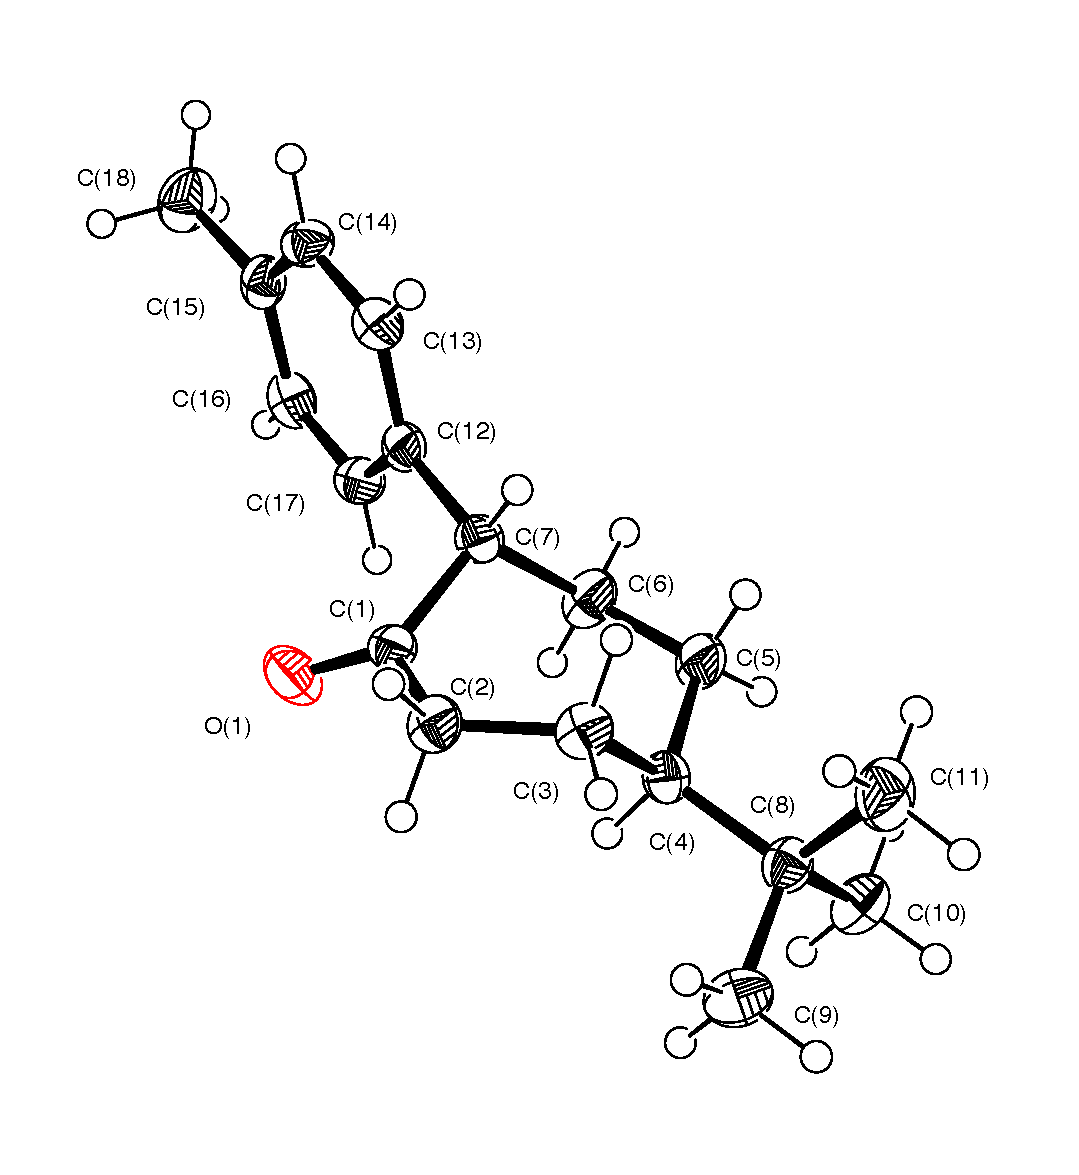
\includegraphics[width=4.5in]{chp_asymmetric/images/xray/xaax_labelled}
    \begin{textblock}{1}(13,-14)
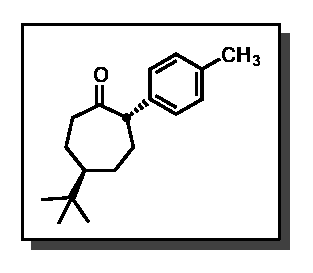
\includegraphics[scale=0.8]{chp_asymmetric/images/xaax}
\end{textblock}
  \caption{ORTEP drawing of ketone ($\pm$)-\ref{cmp:xaay} shown at 50\% probability }
\end{figure}
\pagebreak
\begin{table}[h]
\centering
\caption{Crystal data and structure refinement for ($\pm$)-\ref{cmp:xaay}} 
\begin{tabular}{ll} 
\toprule
Empirical formula& 	C$_{18}$H$_{26}$O \\
Formula weight&	258.39 \\
Temperature &	143(2) K \\
Wavelength& 	0.71073 \AA  \\
Crystal system& 	Orthorhombic \\
Space group& 	Pbca \\
Unit cell dimensions&	a = 19.6684(17) \AA	$\alpha$ = 90$^\circ$. \\
	&b = 6.0152(5) \AA	$\beta$ = 90$^\circ$. \\
	&c = 26.140(2) \AA	$\gamma$ = 90$^\circ$. \\
Volume&	3092.6(5) \AA$^3$ \\
Z&	8 \\
Density (calculated)&	1.110 Mg/m$^3$ \\
Absorption coefficient&	0.066 mm$^{-1}$ \\
F(000) &	1136 \\
Crystal size &	0.25 x 0.12 x 0.09 mm$^3$ \\
Theta range for data collection &	1.56 to 28.00$^\circ$. \\
Index ranges &	$-$23$<=$h$<=$25, $-$7$<=$k$<=$7, $-$34$<=$l$<=$33 \\
Reflections collected &	46273 \\
Independent reflections &	3712 [R(int) = 0.0335] \\
Completeness to theta = 28.00$^\circ$ &	99.8 \% \\ 
Absorption correction&	Semi-empirical from equivalents \\
Max. and min. transmission &	0.9941 and 0.9837 \\
Refinement method	&Full-matrix least-squares on F$^2$ \\
Data / restraints / parameters &	 3712 / 0 / 173 \\
Goodness-of-fit on F$^2$ & 	1.036 \\
Final R indices [I$>$2sigma(I)] &	R1 = 0.0525, wR2 = 0.1434 \\
R indices (all data) &	R1 = 0.0694, wR2 = 0.1573 \\
Extinction coefficient	& na \\
Largest diff. peak and hole &	0.356 and $-$0.227 e.\AA$^{-3}$ \\
\bottomrule
\end{tabular}
\end{table}
\pagebreak

\twocolumn
\begin{table}[h]
\centering
\caption{Atomic coordinates (x 10$^4$) and equivalent isotropic displacement parameters (\AA$^2$x
10$^3$) for ($\pm$)-\ref{cmp:xaay}}
{\footnotesize
\begin{tabular}{lcccc} 
\\
\toprule
& x & y & z & U(eq) \\
\midrule
O(1)&	424(1)&	12639(2)&	2146(1)&	42(1) \\
C(1)&	541(1)&	10709(3)&	2059(1)&	26(1) \\ 
C(2)&	92(1)&	9443(3)&	1692(1)&	32(1) \\
C(3)&	400(1)&	7468(3)&	1416(1)&	31(1) \\
C(4)&	1068(1)&	7957(3)&	1134(1)&	26(1) \\
C(5)&	1672(1)&	7656(3)&	1495(1)&	36(1) \\
C(6)&	1729(1)&	9334(3)&	1929(1)&	36(1) \\
C(7)&	1130(1)&	9475(3)&	2312(1)&	26(1) \\
C(8)&	1135(1)&	6647(3)&	624(1)&	30(1) \\
C(9)&	569(1)&	7416(3)&	253(1)&	42(1) \\
C(10)&	1812(1)&	7186(3)&	357(1)&	40(1) \\
C(11)&	1083(1)&	4156(3)&	705(1)&	48(1) \\
C(12)&	1341(1)&	10598(3)&	2806(1)&	26(1) \\
C(13)&	1196(1)&	9596(3)&	3270(1)&	28(1) \\
C(14)&	1363(1)&	10621(3)&	3727(1)&	30(1) \\
C(15)&	1676(1)&	12680(3)&	3739(1)&	30(1) \\
C(16)&	1838(1)&	13671(3)&	3274(1)&	31(1) \\
C(17)&	1669(1)&	12644(3)&	2814(1)&	30(1) \\
C(18)&	1832(1)&	13845(4)&	4236(1)&	46(1)\\
\bottomrule
\end{tabular}
}
\end{table} 


\begin{center}
\tablefirsthead{%
\toprule}
\tablehead{%
\multicolumn{2}{c}{\footnotesize \textbf{Table \thetable} continued\ldots} \\
\toprule
}
\tabletail{%
%\midrule
\multicolumn{2}{c}{\small \ldots}\\
}
\tablelasttail{\bottomrule}
\topcaption{Bond lengths (\AA) and angles (${^\circ}$) for ($\pm$)-\ref{cmp:xaay}}
{\footnotesize \singlespacing
\begin{supertabular}{p{1.5in}c}
O(1)-C(1) 	&1.2054(19) \\
C(1)-C(2) 	&1.510(2) \\
C(1)-C(7) 	&1.528(2) \\
C(2)-C(3) 	&1.516(2) \\
C(2)-H(2A) &	0.9900 \\
C(2)-H(2B) &	0.9900\\
C(3)-C(4) 	&1.536(2)\\ 
C(3)-H(3A) &	0.9900 \\
C(3)-H(3B) &	0.9900 \\
C(4)-C(5) 	&1.528(2) \\
C(4)-C(8) 	&1.555(2) \\
C(4)-H(4A) &	1.0000 \\
C(5)-C(6) 	&1.523(2) \\
C(5)-H(5A) &	0.9900 \\
C(5)-H(5B) &	0.9900 \\
C(6)-C(7) 	&1.547(2) \\
C(6)-H(6A) &	0.9900 \\
C(6)-H(6B) &	0.9900 \\
C(7)-C(12) &	1.514(2) \\
C(7)-H(7A) &	1.0000\\ 
C(8)-C(11) &	1.517(2)\\ 
C(8)-C(10) &	1.537(2) \\
C(8)-C(9) 	&1.545(2)\\ 
C(9)-H(9A) &	0.9800 \\
C(9)-H(9B) &	0.9800 \\
C(9)-H(9C) &	0.9800 \\
C(10)-H(10A)& 	0.9800 \\
C(10)-H(10B) &	0.9800 \\
C(10)-H(10C) &	0.9800 \\
C(11)-H(11A) &	0.9800 \\
C(11)-H(11B) 	&0.9800 \\
C(11)-H(11C) &	0.9800 \\
C(12)-C(13) &	1.386(2) \\
C(12)-C(17) &	1.390(2) \\
C(13)-C(14) 	&1.384(2) \\
C(13)-H(13A) &	0.9500 \\
C(14)-C(15) &	1.383(2) \\
C(14)-H(14A) &	0.9500 \\
C(15)-C(16) &	1.391(2) \\
C(15)-C(18) 	&1.508(2) \\
C(16)-C(17) &	1.391(2) \\
C(16)-H(16A) &	0.9500 \\
C(17)-H(17A) &	0.9500 \\
C(18)-H(18A) &	0.9800 \\
C(18)-H(18B) &	0.9800 \\
C(18)-H(18C) &	0.9800 \\
O(1)-C(1)-C(2)	&119.60(14) \\
O(1)-C(1)-C(7)	&122.09(14) \\
C(2)-C(1)-C(7)	&118.30(13) \\
C(1)-C(2)-C(3)	&117.65(13) \\
C(1)-C(2)-H(2A)&	107.9 \\
C(3)-C(2)-H(2A)&	107.9 \\
C(1)-C(2)-H(2B)&	107.9 \\
C(3)-C(2)-H(2B)&	107.9 \\
H(2A)-C(2)-H(2B)&	107.2 \\
C(2)-C(3)-C(4)&	114.83(13) \\
C(2)-C(3)-H(3A)&	108.6 \\
C(4)-C(3)-H(3A)&	108.6 \\
C(2)-C(3)-H(3B)&	108.6 \\ 
C(4)-C(3)-H(3B)&	108.6 \\
H(3A)-C(3)-H(3B)&	107.5 \\
C(5)-C(4)-C(3)&	110.28(13) \\
C(5)-C(4)-C(8)&	113.84(12) \\
C(3)-C(4)-C(8)&	112.74(12) \\
C(5)-C(4)-H(4A)&	106.5 \\
C(3)-C(4)-H(4A)&	106.5 \\
C(8)-C(4)-H(4A)&	106.5 \\
C(6)-C(5)-C(4)&	115.99(13) \\
C(6)-C(5)-H(5A)&	108.3 \\
C(4)-C(5)-H(5A)&	108.3 \\
C(6)-C(5)-H(5B)&	108.3 \\
C(4)-C(5)-H(5B)&	108.3 \\
H(5A)-C(5)-H(5B)&	107.4 \\
C(5)-C(6)-C(7)&	117.59(14) \\
C(5)-C(6)-H(6A)&	107.9 \\
C(7)-C(6)-H(6A)&	107.9 \\
C(5)-C(6)-H(6B)&	107.9 \\
C(7)-C(6)-H(6B)&	107.9 \\
H(6A)-C(6)-H(6B)&	107.2 \\
C(12)-C(7)-C(1)&	111.09(12) \\
C(12)-C(7)-C(6)&	111.56(12) \\
C(1)-C(7)-C(6)&	108.90(12) \\
C(12)-C(7)-H(7A)&	108.4 \\
C(1)-C(7)-H(7A)&	108.4 \\
C(6)-C(7)-H(7A)&	108.4 \\
C(11)-C(8)-C(10)&	109.29(15) \\
C(11)-C(8)-C(9)&	109.61(15) \\
C(10)-C(8)-C(9)&	106.04(14) \\
C(11)-C(8)-C(4)&	111.97(14) \\
C(10)-C(8)-C(4)&	110.76(13) \\
C(9)-C(8)-C(4)&	108.99(13) \\
C(8)-C(9)-H(9A)&	109.5 \\
C(8)-C(9)-H(9B)&	109.5 \\
H(9A)-C(9)-H(9B)&	109.5 \\
C(8)-C(9)-H(9C)	&109.5 \\
H(9A)-C(9)-H(9C)&	109.5 \\
H(9B)-C(9)-H(9C)&	109.5 \\
C(8)-C(10)-H(10A)&	109.5 \\
C(8)-C(10)-H(10B)&	109.5 \\
H(10A)-C(10)-H(10B)&	109.5 \\
C(8)-C(10)-H(10C)&	109.5 \\
H(10A)-C(10)-H(10C)&	109.5 \\
H(10B)-C(10)-H(10C)&	109.5 \\
C(8)-C(11)-H(11A)&	109.5 \\
C(8)-C(11)-H(11B)	&109.5 \\
H(11A)-C(11)-H(11B)&	109.5 \\
C(8)-C(11)-H(11C)&	109.5 \\
H(11A)-C(11)-H(11C)&	109.5 \\
H(11B)-C(11)-H(11C)&	109.5 \\ 
C(13)-C(12)-C(17)&	117.80(14)\\ 
C(13)-C(12)-C(7)&	119.78(14)\\
C(17)-C(12)-C(7)&	122.41(14) \\
C(14)-C(13)-C(12)&	120.94(15)\\
C(14)-C(13)-H(13A)&	119.5\\
C(12)-C(13)-H(13A)	&119.5\\
C(15)-C(14)-C(13)&	121.56(15)\\
C(15)-C(14)-H(14A)&	119.2\\
C(13)-C(14)-H(14A)	&119.2\\
C(14)-C(15)-C(16)&	117.79(14)\\
C(14)-C(15)-C(18)&	121.72(16)\\
C(16)-C(15)-C(18)&	120.49(16)\\
C(17)-C(16)-C(15)&	120.68(15)\\
C(17)-C(16)-H(16A)&	119.7\\
C(15)-C(16)-H(16A)&	119.7\\
C(12)-C(17)-C(16)&	121.19(14)\\
C(12)-C(17)-H(17A)&	119.4\\
C(16)-C(17)-H(17A)&	119.4\\
C(15)-C(18)-H(18A)&	109.5\\
C(15)-C(18)-H(18B)&	109.5\\
H(18A)-C(18)-H(18B)&	109.5 \\
C(15)-C(18)-H(18C)	&109.5 \\
H(18A)-C(18)-H(18C)&	109.5 \\
H(18B)-C(18)-H(18C)&	109.5\\
\end{supertabular}
}
\end{center}


\begin{center}
\tablefirsthead{%
\toprule
&x&y&z&U(eq) \\
\midrule}
\tablehead{%
\multicolumn{5}{c}{\footnotesize \textbf{Table \thetable} continued\ldots} \\
\toprule
&x&y&z&U(eq) \\
\midrule
}
\tabletail{%
%\midrule
\multicolumn{5}{c}{\small \ldots}\\
}
\tablelasttail{\bottomrule}
\topcaption{Hydrogen coordinates (x 10$^4$) and isotropic displacement parameters (\AA$^2$x 10$^3$)
for ($\pm$)-\ref{cmp:xaay}} {\footnotesize \singlespacing
\begin{supertabular}{lcccc}
H(2A)&	$-$74&		10502&	1430		&38 \\
H(2B)&	$-$310&	8911&	1884	 	&38\\ 
H(3A)&	65&	6902	& 1165				&37\\
H(3B)&	483&	6272	&1668			&37\\
H(4A)&	1057	& 9569&	1040			&32\\
H(5A)&	1646	& 6149&	1646				&44\\
H(5B)&	2095&	7728	&1290				&44\\
H(6A)&	1792&	10825&	1776			&44\\
H(6B)&	2146&	8989&	2126				&44\\
H(7A)&	977&	7929&	2393				&32\\
H(9A)&	609&	6601	&$-$70				&63\\
H(9B)&	617&	9013	&188				&63\\
H(9C)&	124&	7121	&406				&63\\
H(10A)&	1843&	6347&	37				&61\\
H(10B)&	2190	&6773&	582				&61\\
H(10C)&	1833	&8782&	283				&61\\
H(11A)&	1128&	3392	&376				&72\\
H(11B)&	641&	3798&	857				&72\\
H(11C)&	1447	&3668&	936				&72\\
H(13A)&	979&	8184&	3275				&34\\
H(14A)&	1260	&9893&	4040				&36\\
H(16A)&	2066&	15063&	3270			&37\\
H(17A)&	1781	&13353&	2501			&36\\
H(18A)&	1494&	15013&	4296			&69\\
H(18B)&	2286&	14511&	4217			&69\\
H(18C)&	1818	&12768&	4517			&69\\
\end{supertabular}
}
\end{center}

\begin{center}
\tablefirsthead{%
\toprule}
\tablehead{%
\multicolumn{2}{c}{\footnotesize \textbf{Table \thetable} continued\ldots} \\
\toprule
}
\tabletail{%
%\midrule
\multicolumn{2}{c}{\small \ldots}\\
}
\tablelasttail{\bottomrule}
\topcaption{Torsion angles ($^{\circ}$) for ($\pm$)-\ref{cmp:xaay}}
{\footnotesize \singlespacing
\begin{supertabular}{p{1.5in}c}
O(1)-C(1)-C(2)-C(3)&	153.87(15) \\
C(7)-C(1)-C(2)-C(3)&	$-$26.5(2) \\
C(1)-C(2)-C(3)-C(4)&	$-$52.70(19) \\
C(2)-C(3)-C(4)-C(5)&	87.59(17) \\
C(2)-C(3)-C(4)-C(8)&	$-$143.93(14) \\
C(3)-C(4)-C(5)-C(6)&	$-$67.65(19) \\
C(8)-C(4)-C(5)-C(6)&	164.48(14) \\
C(4)-C(5)-C(6)-C(7)&	59.7(2) \\
O(1)-C(1)-C(7)-C(12)&	22.7(2) \\
C(2)-C(1)-C(7)-C(12)&	$-$156.93(13) \\
O(1)-C(1)-C(7)-C(6)&	$-$100.59(17) \\
C(2)-C(1)-C(7)-C(6)&	79.82(16) \\
C(5)-C(6)-C(7)-C(12)&	161.27(14) \\
C(5)-C(6)-C(7)-C(1)&	$-$75.76(18) \\
C(5)-C(4)-C(8)-C(11)&	69.06(19) \\
C(3)-C(4)-C(8)-C(11)&	$-$57.54(19) \\
C(5)-C(4)-C(8)-C(10)&	$-$53.21(18) \\
C(3)-C(4)-C(8)-C(10)&	$-$179.80(14) \\
C(5)-C(4)-C(8)-C(9)&	$-$169.50(14) \\
C(3)-C(4)-C(8)-C(9)&	63.90(17) \\
C(1)-C(7)-C(12)-C(13)&	108.50(16) \\
C(6)-C(7)-C(12)-C(13)&	$-$129.79(15) \\
C(1)-C(7)-C(12)-C(17)&	$-$70.50(17) \\
C(6)-C(7)-C(12)-C(17)&	51.21(19) \\
C(17)-C(12)-C(13)-C(14)&	1.2(2) \\
C(7)-C(12)-C(13)-C(14)&	$-$177.87(14) \\
C(12)-C(13)-C(14)-C(15)&	0.3(2) \\
C(13)-C(14)-C(15)-C(16)&	$-$1.9(2) \\
C(13)-C(14)-C(15)-C(18)&	177.46(16) \\
C(14)-C(15)-C(16)-C(17)&	2.0(2) \\
C(18)-C(15)-C(16)-C(17)&	$-$177.37(15) \\
C(13)-C(12)-C(17)-C(16)&	$-$1.1(2) \\
C(7)-C(12)-C(17)-C(16)&	177.95(14) \\
C(15)-C(16)-C(17)-C(12)&	$-$0.5(2) \\
\end{supertabular}
}
\end{center}




\onecolumn
\begin{table}[h]
\centering
\footnotesize
\caption{Anisotropic displacement parameters (\AA$^2$x 10$^3$) for ($\pm$)-\ref{cmp:xaay}} 
\begin{tabular}{p{1in}cccccc} 
\toprule
& U$^{11}$ & U$^{22}$ & U$^{33}$ & U$^{23}$ & U$^{13}$ & U$^{12}$ \\
\midrule
O(1)&	48(1) &	31(1)&	48(1) &	$-$1(1)&	$-$13(1) &	10(1) \\
C(1)&	22(1) &	31(1)&	24(1) &	5(1)&	3(1)& 	2(1)\\
C(2)&	20(1) &	42(1)&	32(1) &	$-$1(1)&	2(1)& 	0(1) \\
C(3)&	26(1) &	35(1)&	31(1) &	0(1)&	1(1)& 	$-$4(1)\\
C(4)& 	24(1) &	26(1)&	29(1) &	$-$2(1)&	1(1) &	1(1)\\
C(5)&	26(1) &	53(1)&	30(1) &	$-$6(1)&	$-$1(1)& 	12(1) \\
C(6)&	20(1) &	58(1)&	32(1) &	$-$8(1)&	0(1)& 	3(1)\\
C(7)&	22(1) &	30(1)&	27(1) &	1(1)&	$-$1(1)& 	2(1) \\
C(8)&	32(1) &	27(1)&	30(1) &	$-$3(1)&	2(1) &	$-$2(1) \\
C(9)&	43(1) &	48(1)&	34(1) &	$-$2(1)&	$-$7(1)& 	$-$5(1) \\
C(10)&	42(1) &	48(1)&	32(1) &	$-$4(1)&	7(1) &	$-$1(1)\\
C(11)&	69(1) &	26(1)&	50(1) &	$-$5(1)&	8(1)& 	$-$2(1)\\
C(12)&	19(1) &	32(1)&	28(1) &	$-$1(1)&	0(1)& 	5(1)\\
C(13)&	23(1) &	29(1)&	33(1) &	1(1)&	$-$1(1) &	$-$1(1) \\
C(14)&	26(1) &	38(1)&	27(1) &	4(1)&	1(1)& 	0(1) \\
C(15)&	23(1) &	36(1)&	32(1) &	$-$6(1)&	$-$2(1) &	3(1) \\
C(16)&	21(1) &	29(1)&	44(1) &	0(1)&	0(1) &	$-$2(1)\\
C(17)&	22(1) &	37(1)&	30(1) &	8(1)&	4(1)& 	2(1) \\
C(18)&	47(1) &	52(1)&	40(1) &	$-$15(1)&	$-$5(1) &	$-$1(1) \\
\bottomrule
\end{tabular}
\end{table}
{ \footnotesize
The anisotropic displacement factor exponent takes the form: 
$-2\pi^2\left[ h^2a*^2U^{11} + ... + 2 h k a* b* U^{12} \right]$ }

\pagebreak
%%%%%%%%%%% End of X-Ray Data for xaax %%%%%%%%%%%%%%%%%%%%

%%%%%%%%%%% Begin  X-Ray Data for xabb %%%%%%%%%%%%%%%%%%%%
\subsection{Structural Data for Ester \ref{cmp:xabb}}
Suitable crystals for X-ray analysis were grown by slow evaporation from a 5\% (v/v) solution of
Et$_2$O in hexanes.
\begin{figure}[h]
  \centering
  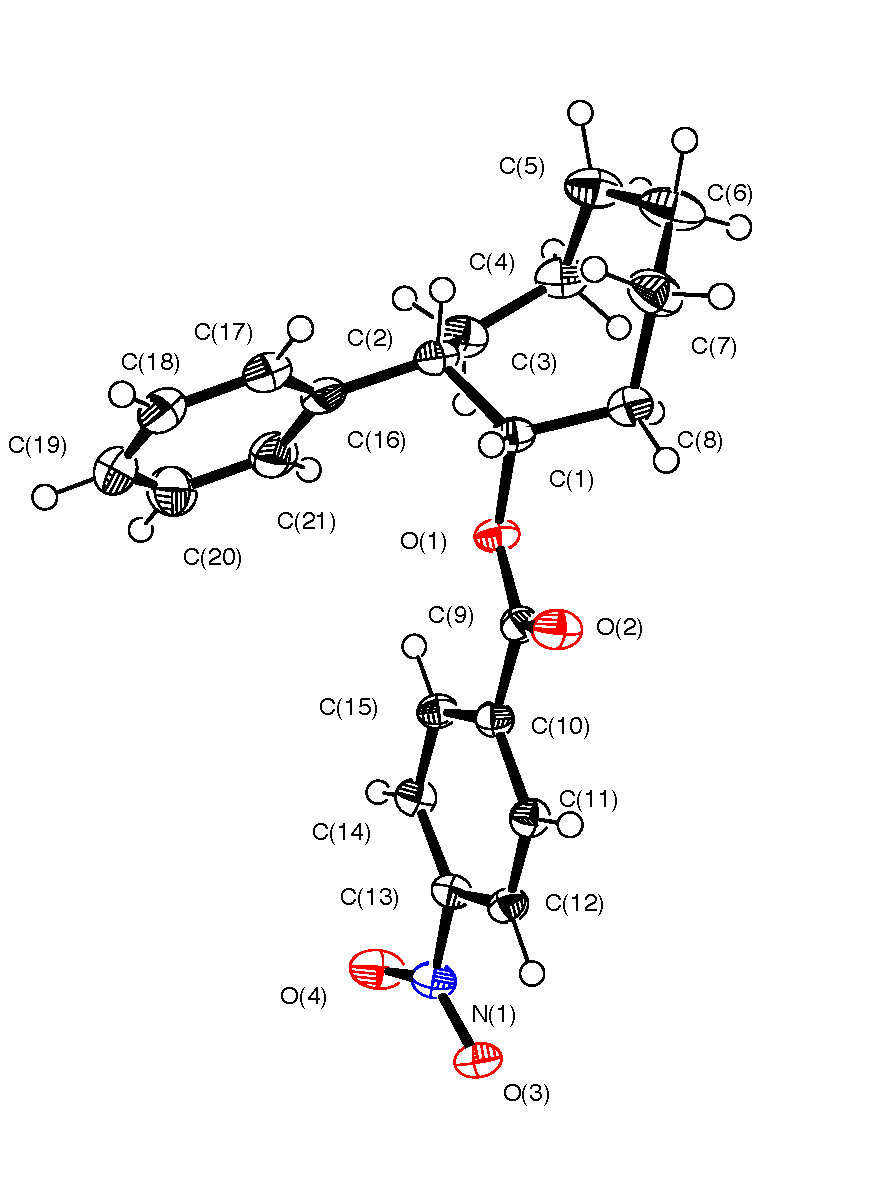
\includegraphics[width=4.2in]{chp_asymmetric/images/xray/xabb_labelled}
  \begin{textblock}{1}(0.5,-8)
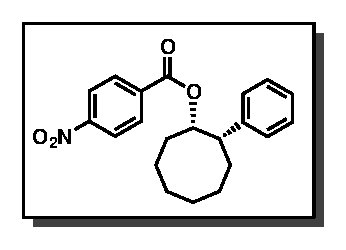
\includegraphics[scale=0.8]{chp_asymmetric/images/xabb}
\end{textblock}
  \caption{ORTEP drawing of ester \ref{cmp:xabb} shown at 50\% probability }
\end{figure}

\pagebreak
\begin{table}[h]
\centering
\caption{Crystal data and structure refinement for \ref{cmp:xabb}} 
\begin{tabular}{ll} 
\toprule
Empirical formula& 	C$_{21}$H$_{23}$NO$_4$ \\
Formula weight&	353.40 \\
Temperature &	100(2) K \\
Wavelength& 	1.54178 \AA  \\
Crystal system& 	Monoclinic \\
Space group& 	P 2(1)/n \\
Unit cell dimensions&	a = 8.4054(10) \AA	$\alpha$ = 90$^\circ$. \\
	&b = 6.9528(8) \AA	$\beta$ = 92.883(4)$^\circ$. \\
	&c = 31.194(4) \AA	$\gamma$ = 90$^\circ$. \\
Volume&	1820.7(4) \AA$^3$ \\
Z&	4 \\
Density (calculated)&	1.289 Mg/m$^3$ \\
Absorption coefficient&	0.723 mm$^{-1}$ \\
F(000) &	752 \\
Crystal size &	0.18 x 0.12 x 0.08 mm$^3$ \\
Theta range for data collection &	5.39 to 67.98$^\circ$. \\
Index ranges &	$-$10$<=$h$<=$9, $-$8$<=$k$<=$5, $-$36$<=$l$<=$37 \\
Reflections collected &	30952 \\
Independent reflections &	3302 [R(int) = 0.0240] \\
Completeness to theta = 67.98$^\circ$ &	99.7 \% \\ 
Absorption correction&	Semi-empirical from equivalents \\
Max. and min. transmission &	0.9444 and 0.8808 \\
Refinement method	&Full-matrix least-squares on F$^2$ \\
Data / restraints / parameters &	 3302 / 3 / 251 \\
Goodness-of-fit on F$^2$ & 	1.054 \\
Final R indices [I$>$2sigma(I)] &	R1 = 0.0426, wR2 = 0.1054 \\
R indices (all data) &	R1 = 0.0432, wR2 = 0.1057 \\
Extinction coefficient	& na \\
Largest diff. peak and hole &	0.493 and $-$0.319 e.\AA$^{-3}$ \\
\bottomrule
\end{tabular}
\end{table}

\pagebreak
\twocolumn

\begin{table}[h]
\centering
\caption{Atomic coordinates (x 10$^4$) and equivalent isotropic displacement parameters (\AA$^2$x
10$^3$) for \ref{cmp:xabb}}
{\footnotesize
\begin{tabular}{lcccc} 
\\
\toprule
& x & y & z & U(eq) \\
\midrule
O(1)&8285(1)&8167(1)&1043(1)&24(1)\\
O(2)&9580(1)&10772(2)&811(1)&31(1)\\
O(3)&13969(1)&4594(2)&-404(1)&31(1)\\
O(4)&13354(1)&2223(2)&4(1)&38(1)\\
N(1)&13281(1)&3919(2)&-100(1)&27(1)\\
C(1)&7295(2)&9388(2)&1304(1)&25(1)\\
C(2)&6756(2)&8094(2)&1667(1)&27(1)\\
C(3)&5660(2)&6435(2)&1517(1)&34(1)\\
C(4)&3967(2)&6922(3)&1326(1)&34(1)\\
C(5)&3099(2)&8562(3)&1532(1)&42(1)\\
C(4X)&3953(10)&6828(14)&1704(3)&34(1)\\
C(5X)&3099(2)&8562(3)&1532(1)&42(1)\\
C(6)&3226(2)&10527(3)&1336(1)&45(1)\\
C(7)&4797(2)&11497(3)&1275(1)&42(1)\\
C(8)&6013(2)&10364(3)&1022(1)&37(1)\\
C(9)&9387(2)&9051(2)&821(1)&23(1)\\
C(10)&10383(2)&7651(2)&586(1)&22(1)\\
C(11)&11411(2)&8393(2)&289(1)&24(1)\\
C(12)&12376(2)&7182(2)&67(1)&24(1)\\
C(13)&12302(2)&5228(2)&149(1)&24(1)\\
C(14)&11322(2)&4448(2)&448(1)&25(1)\\
C(15)&10348(2)&5680(2)&665(1)&24(1)\\
C(16)&8218(2)&7408(2)&1934(1)&32(1)\\
C(17)&8895(2)&8599(3)&2251(1)&38(1)\\
C(18)&10270(2)&8049(3)&2489(1)&48(1)\\
C(19)&10974(2)&6306(3)&2417(1)&52(1)\\
C(20)&10307(2)&5093(3)&2108(1)&52(1)\\
C(21)&8938(2)&5637(3)&1866(1)&41(1)\\
\bottomrule
\end{tabular}
}
\end{table} 

\begin{center}
\tablefirsthead{%
\toprule}
\tablehead{%
\multicolumn{2}{c}{\footnotesize \textbf{Table \thetable} continued\ldots} \\
\toprule
}
\tabletail{%
%\midrule
\multicolumn{2}{c}{\small \ldots}\\
}
\tablelasttail{\bottomrule}
\topcaption{Bond lengths (\AA) and angles (${^\circ}$) for \ref{cmp:xabb}}
{\footnotesize \singlespacing
\begin{supertabular}{p{1.5in}c}
O(1)-C(9)&1.3344(17)\\
O(1)-C(1)&1.4654(16)\\
O(2)-C(9)&1.2085(18)\\
O(3)-N(1)&1.2291(16)\\
O(4)-N(1)&1.2246(17)\\
N(1)-C(13)&1.4742(18)\\
C(1)-C(8)&1.517(2)\\
C(1)-C(2)&1.531(2)\\
C(1)-H(1)&0.971(18)\\
C(2)-C(16)&1.526(2)\\
C(2)-C(3)&1.534(2)\\
C(2)-H(2)&0.984(18)\\
C(3)-C(4)&1.552(3)\\
C(3)-H(3A)&0.99\\
C(3)-H(3B)&0.99\\
C(4)-C(5)&1.513(3)\\
C(4)-H(4A)&0.99\\
C(4)-H(4B)&0.99\\
C(5)-C(6)&1.503(3)\\
C(5)-H(5A)&0.99\\
C(5)-H(5B)&0.99\\
C(6)-C(7)&1.503(2)\\
C(6)-H(6A)&0.99\\
C(6)-H(6B)&0.99\\
C(7)-C(8)&1.539(2)\\
C(7)-H(7A)&0.99\\
C(7)-H(7B)&0.99\\
C(8)-H(8A)&0.939(15)\\
C(8)-H(8B)&0.995(15)\\
C(9)-C(10)&1.4978(19)\\
C(10)-C(15)&1.393(2)\\
C(10)-C(11)&1.3966(19)\\
C(11)-C(12)&1.380(2)\\
C(11)-H(11)&0.95\\
C(12)-C(13)&1.385(2)\\
C(12)-H(12)&0.95\\
C(13)-C(14)&1.385(2)\\
C(14)-C(15)&1.386(2)\\
C(14)-H(14)&0.95\\
C(15)-H(15)&0.95\\
C(16)-C(17)&1.390(2)\\
C(16)-C(21)&1.393(2)\\
C(17)-C(18)&1.396(3)\\
C(17)-H(17)&0.95\\
C(18)-C(19)&1.373(3)\\
C(18)-H(18)&0.95\\
C(19)-C(20)&1.378(3)\\
C(19)-H(19)&0.95\\
C(20)-C(21)&1.396(3)\\
C(20)-H(20)&0.95\\
C(21)-H(21)&0.95\\
C(9)-O(1)-C(1)&116.79(11)\\
O(4)-N(1)-O(3)&123.65(12)\\
O(4)-N(1)-C(13)&118.43(12)\\
O(3)-N(1)-C(13)&117.93(12)\\
O(1)-C(1)-C(8)&110.06(12)\\
O(1)-C(1)-C(2)&105.54(11)\\
C(8)-C(1)-C(2)&117.60(13)\\
O(1)-C(1)-H(1)&107.5(10)\\
C(8)-C(1)-H(1)&106.9(10)\\
C(2)-C(1)-H(1)&108.9(10)\\
C(16)-C(2)-C(1)&109.05(12)\\
C(16)-C(2)-C(3)&112.69(13)\\
C(1)-C(2)-C(3)&114.39(13)\\
C(16)-C(2)-H(2)&106.1(10)\\
C(1)-C(2)-H(2)&106.0(10)\\
C(3)-C(2)-H(2)&108.1(10)\\
C(2)-C(3)-C(4)&118.51(14)\\
C(2)-C(3)-H(3A)&107.7\\
C(4)-C(3)-H(3A)&107.7\\
C(2)-C(3)-H(3B)&107.7\\
C(4)-C(3)-H(3B)&107.7\\
H(3A)-C(3)-H(3B)&107.1\\
C(5)-C(4)-C(3)&117.02(15)\\
C(5)-C(4)-H(4A)&108\\
C(3)-C(4)-H(4A)&108\\
C(5)-C(4)-H(4B)&108\\
C(3)-C(4)-H(4B)&108\\
H(4A)-C(4)-H(4B)&107.3\\
C(6)-C(5)-C(4)&117.78(15)\\
C(6)-C(5)-H(5A)&107.9\\
C(4)-C(5)-H(5A)&107.9\\
C(6)-C(5)-H(5B)&107.9\\
C(4)-C(5)-H(5B)&107.9\\
H(5A)-C(5)-H(5B)&107.2\\
C(7)-C(6)-C(5)&122.72(17)\\
C(7)-C(6)-H(6A)&106.7\\
C(5)-C(6)-H(6A)&106.7\\
C(7)-C(6)-H(6B)&106.7\\
C(5)-C(6)-H(6B)&106.7\\
H(6A)-C(6)-H(6B)&106.6\\
C(6)-C(7)-C(8)&116.44(16)\\
C(6)-C(7)-H(7A)&108.2\\
C(8)-C(7)-H(7A)&108.2\\
C(6)-C(7)-H(7B)&108.2\\
C(8)-C(7)-H(7B)&108.2\\
H(7A)-C(7)-H(7B)&107.3\\
C(1)-C(8)-C(7)&113.75(14)\\
C(1)-C(8)-H(8A)&106.7(13)\\
C(7)-C(8)-H(8A)&110.7(12)\\
C(1)-C(8)-H(8B)&105.2(12)\\
C(7)-C(8)-H(8B)&108.5(12)\\
H(8A)-C(8)-H(8B)&111.9(17)\\
O(2)-C(9)-O(1)&124.55(13)\\
O(2)-C(9)-C(10)&123.48(13)\\
O(1)-C(9)-C(10)&111.96(12)\\
C(15)-C(10)-C(11)&119.99(13)\\
C(15)-C(10)-C(9)&122.38(13)\\
C(11)-C(10)-C(9)&117.59(13)\\
C(12)-C(11)-C(10)&120.46(13)\\
C(12)-C(11)-H(11)&119.8\\
C(10)-C(11)-H(11)&119.8\\
C(11)-C(12)-C(13)&118.18(13)\\
C(11)-C(12)-H(12)&120.9\\
C(13)-C(12)-H(12)&120.9\\
C(14)-C(13)-C(12)&122.86(13)\\
C(14)-C(13)-N(1)&118.67(13)\\
C(12)-C(13)-N(1)&118.45(13)\\
C(13)-C(14)-C(15)&118.26(13)\\
C(13)-C(14)-H(14)&120.9\\
C(15)-C(14)-H(14)&120.9\\
C(14)-C(15)-C(10)&120.22(13)\\
C(14)-C(15)-H(15)&119.9\\
C(10)-C(15)-H(15)&119.9\\
C(17)-C(16)-C(21)&117.95(16)\\
C(17)-C(16)-C(2)&119.48(15)\\
C(21)-C(16)-C(2)&122.55(15)\\
C(16)-C(17)-C(18)&120.98(18)\\
C(16)-C(17)-H(17)&119.5\\
C(18)-C(17)-H(17)&119.5\\
C(19)-C(18)-C(17)&120.39(19)\\
C(19)-C(18)-H(18)&119.8\\
C(17)-C(18)-H(18)&119.8\\
C(18)-C(19)-C(20)&119.50(18)\\
C(18)-C(19)-H(19)&120.3\\
C(20)-C(19)-H(19)&120.3\\
C(19)-C(20)-C(21)&120.46(19)\\
C(19)-C(20)-H(20)&119.8\\
C(21)-C(20)-H(20)&119.8\\
C(16)-C(21)-C(20)&120.71(19)\\
C(16)-C(21)-H(21)&119.6\\
C(20)-C(21)-H(21)&119.6\\
\end{supertabular}
}
\end{center}

\pagebreak

\begin{center}
\tablefirsthead{%
\toprule
&x&y&z&U(eq) \\
\midrule}
\tablehead{%
\multicolumn{5}{c}{\footnotesize \textbf{Table \thetable} continued\ldots} \\
\toprule
&x&y&z&U(eq) \\
\midrule
}
\tabletail{%
%\midrule
\multicolumn{5}{c}{\small \ldots}\\
}
\tablelasttail{\bottomrule}
\topcaption{Hydrogen coordinates (x 10$^4$) and isotropic displacement parameters (\AA$^2$x 10$^3$)
for \ref{cmp:xabb}} {\footnotesize \singlespacing
\begin{supertabular}{lcccc}
H(1)&7970(20)&10400(30)&1427(5)&30\\
H(2)&6160(20)&8930(30)&1856(6)&32\\
H(3A)&5538&5568&1765&41\\
H(3B)&6215&5695&1298&41\\
H(4A)&4051&7227&1018&41\\
H(4B)&3301&5753&1343&41\\
H(5A)&1956&8219&1531&50\\
H(5B)&3494&8650&1836&50\\
H(4C)&3271&5689&1644&41\\
H(4D)&4092&6959&2020&41\\
H(5C)&2438&8867&1777&50\\
H(5D)&2346&7949&1319&50\\
H(6A)&2667&10462&1049&54\\
H(6B)&2600&11408&1511&54\\
H(7A)&5291&11798&1562&50\\
H(7B)&4586&12735&1126&50\\
H(8A)&5500(20)&9390(30)&857(6)&45\\
H(8B)&6590(20)&11280(30)&841(6)&45\\
H(11)&11445&9741&240&29\\
H(12)&13072&7676&-137&29\\
H(14)&11317&3104&502&30\\
H(15)&9654&5179&869&29\\
H(17)&8415&9805&2306&45\\
H(18)&10722&8887&2703&58\\
H(19)&11914&5938&2578&62\\
H(20)&10782&3877&2059&62\\
H(21)&8493&4791&1653&49\\
\end{supertabular}
}
\end{center}

\begin{center}
\tablefirsthead{%
\toprule}
\tablehead{%
\multicolumn{2}{c}{\footnotesize \textbf{Table \thetable} continued\ldots} \\
\toprule
}
\tabletail{%
%\midrule
\multicolumn{2}{c}{\small \ldots}\\
}
\tablelasttail{\bottomrule}
\topcaption{Torsion angles ($^{\circ}$) for \ref{cmp:xabb}}
{\footnotesize \singlespacing
\begin{supertabular}{p{1.5in}c}
C(9)-O(1)-C(1)-C(8)&78.24(16)\\
C(9)-O(1)-C(1)-C(2)&$-$153.92(12)\\
O(1)-C(1)-C(2)-C(16)&61.89(15)\\
C(8)-C(1)-C(2)-C(16)&$-$174.94(14)\\
O(1)-C(1)-C(2)-C(3)&$-$65.31(15)\\
C(8)-C(1)-C(2)-C(3)&57.86(18)\\
C(16)-C(2)-C(3)-C(4)&167.37(14)\\
C(1)-C(2)-C(3)-C(4)&$-$67.32(18)\\
C(2)-C(3)-C(4)-C(5)&$-$38.0(2)\\
C(3)-C(4)-C(5)-C(6)&94.4(2)\\
C(4)-C(5)-C(6)-C(7)&$-$56.4(3)\\
C(5)-C(6)-C(7)-C(8)&54.8(3)\\
O(1)-C(1)-C(8)-C(7)&173.43(13)\\
C(2)-C(1)-C(8)-C(7)&52.6(2)\\
C(6)-C(7)-C(8)-C(1)&$-$100.5(2)\\
C(1)-O(1)-C(9)-O(2)&$-$2.5(2)\\
C(1)-O(1)-C(9)-C(10)&176.73(11)\\
O(2)-C(9)-C(10)-C(15)&167.47(14)\\
O(1)-C(9)-C(10)-C(15)&$-$11.80(19)\\
O(2)-C(9)-C(10)-C(11)&$-$10.5(2)\\
O(1)-C(9)-C(10)-C(11)&170.19(12)\\
C(15)-C(10)-C(11)-C(12)&1.1(2)\\
C(9)-C(10)-C(11)-C(12)&179.17(13)\\
C(10)-C(11)-C(12)-C(13)&$-$0.5(2)\\
C(11)-C(12)-C(13)-C(14)&$-$0.9(2)\\
C(11)-C(12)-C(13)-N(1)&177.51(12)\\
O(4)-N(1)-C(13)-C(14)&$-$9.6(2)\\
O(3)-N(1)-C(13)-C(14)&169.86(13)\\
O(4)-N(1)-C(13)-C(12)&171.97(14)\\
O(3)-N(1)-C(13)-C(12)&$-$8.57(19)\\
C(12)-C(13)-C(14)-C(15)&1.5(2)\\
N(1)-C(13)-C(14)-C(15)&$-$176.84(12)\\
C(13)-C(14)-C(15)-C(10)&$-$0.8(2)\\
C(11)-C(10)-C(15)-C(14)&$-$0.4(2)\\
C(9)-C(10)-C(15)-C(14)&$-$178.39(12)\\
C(1)-C(2)-C(16)-C(17)&82.23(16)\\
C(3)-C(2)-C(16)-C(17)&$-$149.60(14)\\
C(1)-C(2)-C(16)-C(21)&$-$96.12(17)\\
C(3)-C(2)-C(16)-C(21)&32.0(2)\\
C(21)-C(16)-C(17)-C(18)&1.0(2)\\
C(2)-C(16)-C(17)-C(18)&$-$177.39(15)\\
C(16)-C(17)-C(18)-C(19)&$-$0.6(3)\\
C(17)-C(18)-C(19)-C(20)&$-$0.4(3)\\
C(18)-C(19)-C(20)-C(21)&0.8(3)\\
C(17)-C(16)-C(21)-C(20)&$-$0.6(2)\\
C(2)-C(16)-C(21)-C(20)&177.78(15)\\
C(19)-C(20)-C(21)-C(16)&$-$0.3(3)\\
\end{supertabular}
}
\end{center}



\onecolumn
\begin{table}[h]
\centering
\footnotesize
\caption{Anisotropic displacement parameters (\AA$^2$x 10$^3$) for \ref{cmp:xabb}} 
\begin{tabular}{p{1in}cccccc} 
\toprule
& U$^{11}$ & U$^{22}$ & U$^{33}$ & U$^{23}$ & U$^{13}$ & U$^{12}$ \\
\midrule
O(1)&26(1)&21(1)&27(1)&$-$2(1)&9(1)&$-$3(1)\\
O(2)&33(1)&20(1)&40(1)&2(1)&13(1)&0(1)\\
O(3)&30(1)&34(1)&29(1)&$-$4(1)&10(1)&$-$4(1)\\
O(4)&38(1)&21(1)&55(1)&$-$3(1)&18(1)&$-$1(1)\\
N(1)&24(1)&24(1)&32(1)&$-$5(1)&5(1)&$-$4(1)\\
C(1)&27(1)&22(1)&27(1)&$-$3(1)&8(1)&$-$1(1)\\
C(2)&28(1)&25(1)&27(1)&$-$1(1)&9(1)&0(1)\\
C(3)&34(1)&25(1)&45(1)&1(1)&11(1)&$-$4(1)\\
C(4)&34(1)&29(1)&40(1)&$-$6(1)&10(1)&$-$9(1)\\
C(5)&32(1)&43(1)&51(1)&$-$2(1)&16(1)&$-$4(1)\\
C(4X)&34(1)&29(1)&40(1)&$-$6(1)&10(1)&$-$9(1)\\
C(5X)&32(1)&43(1)&51(1)&$-$2(1)&16(1)&$-$4(1)\\
C(6)&37(1)&35(1)&65(1)&$-$15(1)&18(1)&0(1)\\
C(7)&36(1)&32(1)&59(1)&4(1)&12(1)&6(1)\\
C(8)&34(1)&46(1)&33(1)&8(1)&10(1)&6(1)\\
C(9)&22(1)&22(1)&24(1)&3(1)&3(1)&$-$2(1) \\
C(10)&21(1)&22(1)&24(1)&$-$1(1)&2(1)&$-$2(1) \\
C(11)&26(1)&20(1)&27(1)&2(1)&3(1)&$-$3(1)\\
C(12)&24(1)&26(1)&25(1)&2(1)&5(1)&$-$4(1)\\
C(13)&21(1)&24(1)&27(1)&$-$4(1)&4(1)&$-$2(1)\\
C(14)&26(1)&19(1)&31(1)&0(1)&3(1)&$-$4(1)\\
C(15)&23(1)&24(1)&26(1)&1(1)&5(1)&$-$4(1)\\
C(16)&32(1)&37(1)&28(1)&8(1)&12(1)&1(1)\\
C(17)&36(1)&51(1)&28(1)&0(1)&9(1)&4(1)\\
C(18)&41(1)&77(2)&27(1)&4(1)&5(1)&3(1)\\
C(19)&44(1)&75(2)&36(1)&21(1)&6(1)&13(1)\\
C(20)&50(1)&51(1)&55(1)&22(1)&13(1)&17(1)\\
C(21)&45(1)&37(1)&40(1)&10(1)&10(1)&6(1)\\
\bottomrule
\end{tabular}
\end{table}
{ \footnotesize
The anisotropic displacement factor exponent takes the form: 
$-2\pi^2\left[ h^2a*^2U^{11} + ... + 2 h k a* b* U^{12} \right]$ }

\pagebreak
%%%%%%%%%%% End of X-Ray Data for xabb %%%%%%%%%%%%%%%%%%%%

%%%%%%%%%%% Begin  X-Ray Data for xabf %%%%%%%%%%%%%%%%%%%%
\subsection{Structural Data for Bis(oxazoline) Triflate Salt \ref{cmp:xabf}}
Suitable crystals for X-ray analysis were grown by layering a \ce{CHCl3} solution containing a 1:1
molar mixture of \ce{Sc(OTf)3} and \ref{cmp:ligandal} with hexanes.
\begin{figure}[h]
 % \centering
  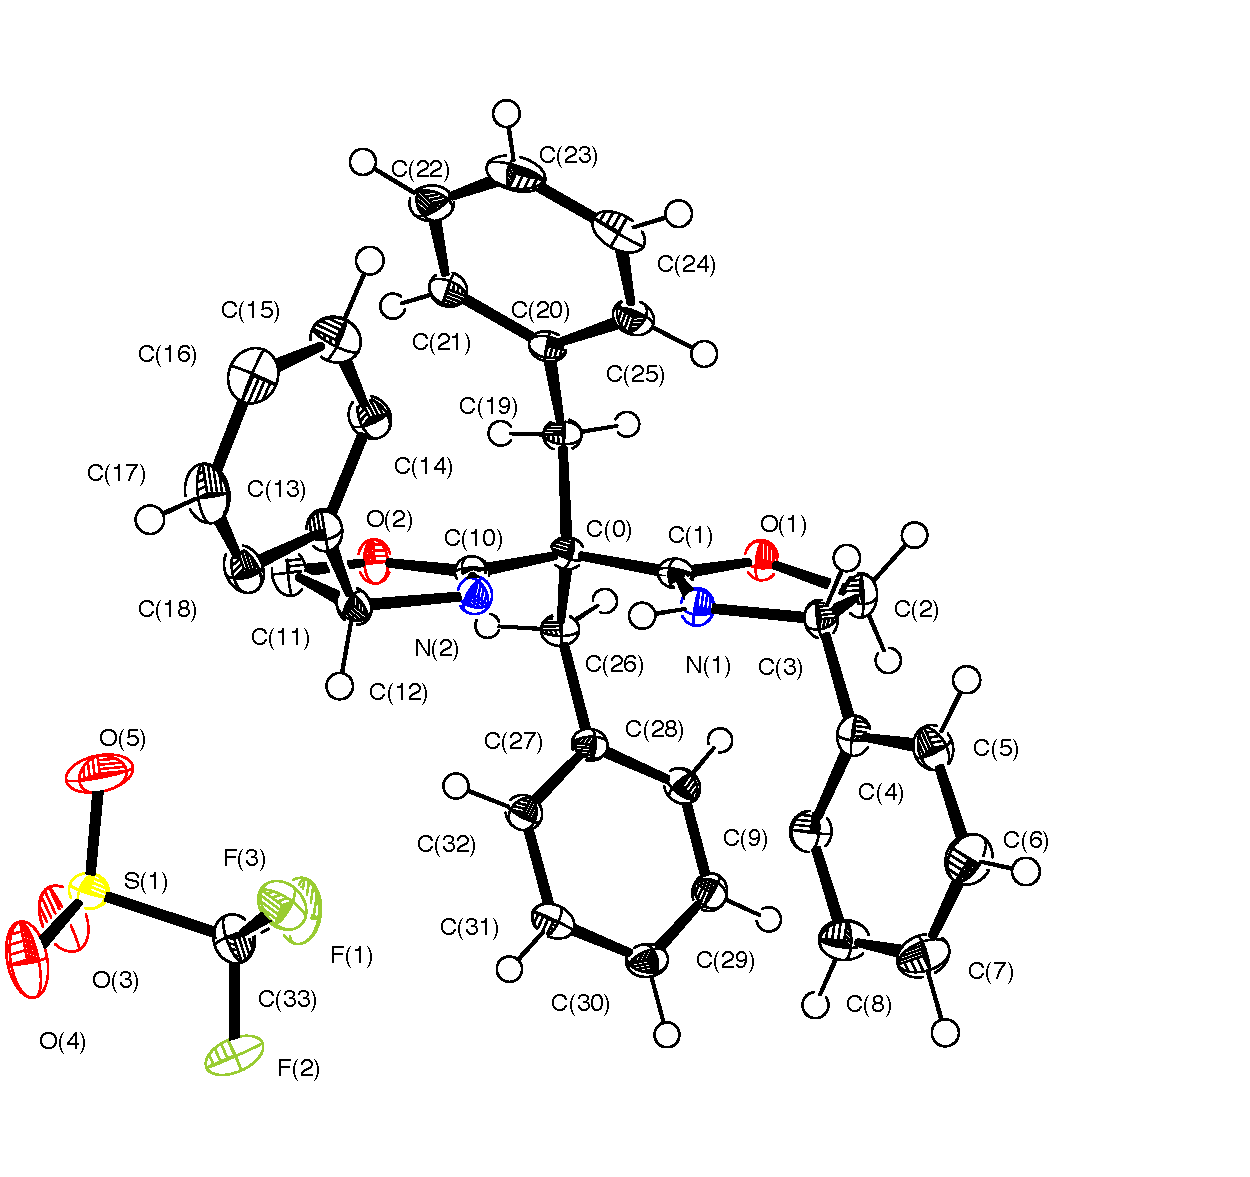
\includegraphics[width=6in]{chp_asymmetric/images/xray/xabf_labelled}
    \begin{textblock}{1}(13,-16)
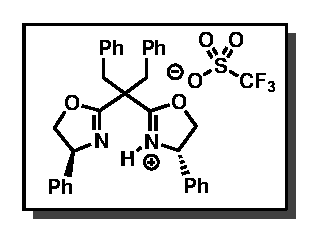
\includegraphics[scale=0.8]{chp_asymmetric/images/xabf}
\end{textblock}
  \caption{ORTEP drawing of bis(oxazoline) triflate salt \ref{cmp:xabf} shown at 50\% probability }
\end{figure}

\pagebreak

\begin{table}[h]
\centering
\caption{Crystal data and structure refinement for \ref{cmp:xabf}} 
\begin{tabular}{ll} 
\toprule
Empirical formula& 	\ce{C35H32Cl3F3N2O5S} \\
Formula weight&	756.04 \\
Temperature &	100(2) K \\
Wavelength& 	0.71073 \AA  \\
Crystal system& 	Monoclinic \\
Space group& 	P 1 21/n 1 \\
Unit cell dimensions&	a = 12.210(3) \AA\ $\alpha$ = 90$^\circ$. \\
	&b = 15.378(4) \AA\	$\beta$ = 102.372(3)$^\circ$. \\
	&c = 19.087(4) \AA\	$\gamma$ = 90$^\circ$. \\
Volume&	3500.7(14) \AA$^3$ \\
Z&	4 \\
Density (calculated)&	1.434 Mg/m$^3$ \\
Absorption coefficient&	0.382 mm$^{-1}$ \\
F(000) &	1560 \\
Crystal size &	0.14 x 0.09 x 0.06 mm$^3$ \\
Theta range for data collection &	2.22 to 28.28$^\circ$. \\
Index ranges &	$-$16$<=$h$<=$16, $-$20$<=$k$<=$20, $-$25$<=$l$<=$24 \\
Reflections collected &	51917 \\
Independent reflections &	8620 [R(int) = 0.0382] \\
Completeness to theta = 28.28$^\circ$ &	99.4\% \\ 
Absorption correction&	Semi-empirical from equivalents \\
Max. and min. transmission &	0.9774 and 0.9484 \\
Refinement method	&Full-matrix least-squares on F$^2$ \\
Data / restraints / parameters &	 8620 / 142 / 566 \\
Goodness-of-fit on F$^2$ & 	1.030 \\
Final R indices [I$>$2sigma(I)] &	R1 = 0.0468, wR2 = 0.1153 \\
R indices (all data) &	R1 = 0.0549, wR2 = 0.1210 \\
Extinction coefficient	& na \\
Largest diff. peak and hole &	0.794 and $-$0.805 e.\AA$^{-3}$ \\
\bottomrule
\end{tabular}
\end{table}

\twocolumn
\begin{center}
\tablefirsthead{%
\toprule
&x&y&z&U(eq) \\
\midrule}
\tablehead{%
\multicolumn{5}{c}{\footnotesize \textbf{Table \thetable} continued\ldots} \\
\toprule
&x&y&z&U(eq) \\
\midrule
}
\tabletail{%
%\midrule
\multicolumn{5}{c}{\small \ldots}\\
}
\tablelasttail{\bottomrule}
\topcaption{Atomic coordinates (x 10$^4$) and equivalent isotropic displacement parameters (\AA$^2$x
10$^3$) for \ref{cmp:xabf}} {\footnotesize \singlespacing
\begin{supertabular}{lcccc}
O(1)&6813(1)&1776(1)&3263(1)&21(1)\\
O(2)&3126(1)&1848(1)&1796(1)&23(1)\\
N(1)&6051(1)&3053(1)&2978(1)&18(1)\\
N(2)&4048(1)&3115(1)&2089(1)&20(1)\\
C(0)&4980(1)&1708(1)&2504(1)&17(1)\\
C(1)&5954(1)&2220(1)&2910(1)&17(1)\\
C(2)&7617(1)&2395(1)&3681(1)&24(1)\\
C(3)&7149(1)&3308(1)&3433(1)&20(1)\\
C(4)&7029(1)&3905(1)&4039(1)&19(1)\\
C(5)&7689(1)&4648(1)&4175(1)&24(1)\\
C(6)&7607(2)&5186(1)&4744(1)&31(1)\\
C(7)&6866(2)&4986(1)&5179(1)&32(1)\\
C(8)&6202(2)&4248(1)&5043(1)&29(1)\\
C(9)&6283(1)&3708(1)&4474(1)&24(1)\\
C(10)&4045(1)&2291(1)&2128(1)&17(1)\\
C(11)&2360(1)&2500(1)&1412(1)&25(1)\\
C(12)&2934(1)&3379(1)&1655(1)&21(1)\\
C(13)&3026(1)&3960(1)&1034(1)&20(1)\\
C(14)&3836(1)&3804(1)&633(1)&24(1)\\
C(15)&3868(2)&4302(1)&33(1)&28(1)\\
C(16)&3100(2)&4969(1)&$-$172(1)&30(1)\\
C(17)&2301(2)&5136(1)&232(1)&30(1)\\
C(18)&2262(1)&4634(1)&828(1)&25(1)\\
C(19)&5369(1)&1118(1)&1936(1)&19(1)\\
C(20)&5589(1)&1598(1)&1291(1)&18(1)\\
C(21)&4864(1)&1496(1)&625(1)&24(1)\\
C(22)&5062(2)&1934(1)&28(1)&30(1)\\
C(23)&5968(2)&2488(1)&89(1)&33(1)\\
C(24)&6694(2)&2595(1)&748(1)&29(1)\\
C(25)&6515(1)&2144(1)&1346(1)&23(1)\\
C(26)&4571(1)&1102(1)&3056(1)&19(1)\\
C(27)&4430(1)&1555(1)&3733(1)&18(1)\\
C(28)&5154(1)&1366(1)&4385(1)&22(1)\\
C(29)&5022(1)&1766(1)&5015(1)&23(1)\\
C(30)&4180(1)&2376(1)&5000(1)&24(1)\\
C(31)&3457(1)&2572(1)&4353(1)&24(1)\\
C(32)&3572(1)&2159(1)&3723(1)&21(1)\\
S(1)&$-$598(1)&3515(1)&2218(1)&25(1)\\
O(3)&$-$1124(1)&2759(1)&2450(1)&44(1)\\
O(4)&$-$1257(1)&4286(1)&2196(1)&45(1)\\
O(5)&$-$48(2)&3371(2)&1647(1)&86(1)\\
C(33)&572(2)&3704(1)&2968(1)&27(1)\\
F(1)&1166(9)&3014(5)&3224(4)&40(2)\\
F(2)&164(7)&4027(3)&3533(3)&33(1)\\
F(3)&1254(11)&4310(10)&2808(11)&31(2)\\
F(1X)&1260(7)&3000(5)&2982(12)&65(3)\\
F(2X)&287(9)&3774(15)&3573(4)&77(3)\\
F(3X)&1219(11)&4379(10)&2888(11)&31(2)\\
C(34)&5330(2)&5825(1)&2459(1)&34(1)\\
Cl(1)&6463(1)&5211(1)&2287(1)&41(1)\\
Cl(2)&4732(1)&5293(1)&3103(1)&60(1)\\
Cl(3)&4331(1)&5975(1)&1660(1)&60(1)\\
\end{supertabular}
}
\end{center}

\begin{center}
\tablefirsthead{%
\toprule}
\tablehead{%
\multicolumn{2}{c}{\footnotesize \textbf{Table \thetable} continued\ldots} \\
\toprule
}
\tabletail{%
%\midrule
\multicolumn{2}{c}{\small \ldots}\\
}
\tablelasttail{\bottomrule}
\topcaption{Bond lengths (\AA) and angles (${^\circ}$) for \ref{cmp:xabf}}
{\footnotesize \singlespacing
\begin{supertabular}{p{1.5in}c}
O(1)-C(1) &1.3102(18)\\
O(1)-C(2) &1.4736(19)\\
O(2)-C(10) &1.3493(18)\\
O(2)-C(11) &1.458(2)\\
N(1)-C(1) &1.291(2)\\
N(1)-C(3) &1.486(2)\\
N(1)-H(1N) &0.866(15)\\
N(2)-C(10) &1.268(2)\\
N(2)-C(12) &1.490(2)\\
C(0)-C(1) &1.497(2)\\
C(0)-C(10) &1.506(2)\\
C(0)-C(19) &1.564(2)\\
C(0)-C(26) &1.567(2)\\
C(2)-C(3) &1.550(2)\\
C(2)-H(2A) &0.983(15)\\
C(2)-H(2B) &0.987(15)\\
C(3)-C(4) &1.509(2)\\
C(3)-H(3) &0.981(14)\\
C(4)-C(5) &1.390(2)\\
C(4)-C(9) &1.391(2)\\
C(5)-C(6) &1.387(2)\\
C(5)-H(5) &0.959(15)\\
C(6)-C(7) &1.387(3)\\
C(6)-H(6) &0.952(16)\\
C(7)-C(8) &1.388(3)\\
C(7)-H(7) &0.945(15)\\
C(8)-C(9) &1.387(2)\\
C(8)-H(8) &0.961(15)\\
C(9)-H(9) &0.945(15)\\
C(11)-C(12) &1.548(2)\\
C(11)-H(11A) &0.978(15)\\
C(11)-H(11B) &0.985(15)\\
C(12)-C(13) &1.507(2)\\
C(12)-H(12) &0.982(14)\\
C(13)-C(18) &1.393(2)\\
C(13)-C(14) &1.395(2)\\
C(14)-C(15) &1.386(2)\\
C(14)-H(14) &0.970(15)\\
C(15)-C(16) &1.388(3)\\
C(15)-H(15) &0.960(15)\\
C(16)-C(17) &1.389(3)\\
C(16)-H(16) &0.951(15)\\
C(17)-C(18) &1.386(3)\\
C(17)-H(17) &0.946(15)\\
C(18)-H(18) &0.955(15)\\
C(19)-C(20) &1.509(2)\\
C(19)-H(19A) &0.970(14)\\
C(19)-H(19B) &0.971(14)\\
C(20)-C(25) &1.394(2)\\
C(20)-C(21) &1.394(2)\\
C(21)-C(22) &1.389(2)\\
C(21)-H(21) &0.947(15)\\
C(22)-C(23) &1.382(3)\\
C(22)-H(22) &0.953(15)\\
C(23)-C(24) &1.385(3)\\
C(23)-H(23) &0.937(16)\\
C(24)-C(25) &1.391(2)\\
C(24)-H(24) &0.933(15)\\
C(25)-H(25) &0.957(15)\\
C(26)-C(27) &1.510(2)\\
C(26)-H(26A) &0.973(14)\\
C(26)-H(26B) &0.981(14)\\
C(27)-C(28) &1.395(2)\\
C(27)-C(32) &1.396(2)\\
C(28)-C(29) &1.391(2)\\
C(28)-H(28) &0.944(14)\\
C(29)-C(30) &1.387(2)\\
C(29)-H(29) &0.955(15)\\
C(30)-C(31) &1.388(3)\\
C(30)-H(30) &0.952(15)\\
C(31)-C(32) &1.394(2)\\
C(31)-H(31) &0.946(15)\\
C(32)-H(32) &0.961(15)\\
S(1)-O(5) &1.4154(16)\\
S(1)-O(4) &1.4273(15)\\
S(1)-O(3) &1.4439(15)\\
S(1)-C(33) &1.8158(19)\\
C(33)-F(2X) &1.281(8)\\
C(33)-F(1) &1.319(7)\\
C(33)-F(3) &1.327(8)\\
C(33)-F(3X) &1.331(9)\\
C(33)-F(1X) &1.366(8)\\
C(33)-F(2) &1.375(5)\\
C(34)-Cl(3) &1.752(2)\\
C(34)-Cl(2) &1.759(2)\\
C(34)-Cl(1) &1.764(2)\\
C(34)-H(34) &0.991(16)\\
C(1)-O(1)-C(2)&107.94(12)\\
C(10)-O(2)-C(11)&105.57(12)\\
C(1)-N(1)-C(3)&111.83(13)\\
C(1)-N(1)-H(1N)&119.5(13)\\
C(3)-N(1)-H(1N)&128.6(13)\\
C(10)-N(2)-C(12)&106.96(13)\\
C(1)-C(0)-C(10)&111.76(12)\\
C(1)-C(0)-C(19)&109.76(12)\\
C(10)-C(0)-C(19)&109.07(12)\\
C(1)-C(0)-C(26)&107.26(12)\\
C(10)-C(0)-C(26)&110.93(12)\\
C(19)-C(0)-C(26)&107.99(12)\\
N(1)-C(1)-O(1)&114.85(14)\\
N(1)-C(1)-C(0)&128.24(14)\\
O(1)-C(1)-C(0)&116.88(13)\\
O(1)-C(2)-C(3)&105.12(12)\\
O(1)-C(2)-H(2A)&107.8(12)\\
C(3)-C(2)-H(2A)&112.8(12)\\
O(1)-C(2)-H(2B)&106.9(12)\\
C(3)-C(2)-H(2B)&113.9(12)\\
H(2A)-C(2)-H(2B)&109.9(17)\\
N(1)-C(3)-C(4)&112.63(12)\\
N(1)-C(3)-C(2)&99.62(12)\\
C(4)-C(3)-C(2)&114.04(13)\\
N(1)-C(3)-H(3)&108.0(12)\\
C(4)-C(3)-H(3)&111.6(11)\\
C(2)-C(3)-H(3)&110.2(12)\\
C(5)-C(4)-C(9)&119.70(15)\\
C(5)-C(4)-C(3)&119.69(14)\\
C(9)-C(4)-C(3)&120.60(14)\\
C(6)-C(5)-C(4)&120.03(16)\\
C(6)-C(5)-H(5)&119.3(13)\\
C(4)-C(5)-H(5)&120.6(13)\\
C(7)-C(6)-C(5)&120.14(16)\\
C(7)-C(6)-H(6)&118.4(14)\\
C(5)-C(6)-H(6)&121.4(14)\\
C(6)-C(7)-C(8)&119.99(16)\\
C(6)-C(7)-H(7)&120.3(14)\\
C(8)-C(7)-H(7)&119.7(14)\\
C(9)-C(8)-C(7)&119.96(16)\\
C(9)-C(8)-H(8)&121.1(13)\\
C(7)-C(8)-H(8)&119.0(13)\\
C(8)-C(9)-C(4)&120.18(15)\\
C(8)-C(9)-H(9)&119.9(12)\\
C(4)-C(9)-H(9)&119.9(12)\\
N(2)-C(10)-O(2)&119.28(14)\\
N(2)-C(10)-C(0)&127.66(14)\\
O(2)-C(10)-C(0)&113.06(12)\\
O(2)-C(11)-C(12)&104.46(12)\\
O(2)-C(11)-H(11A)&106.5(12)\\
C(12)-C(11)-H(11A)&114.5(12)\\
O(2)-C(11)-H(11B)&106.4(12)\\
C(12)-C(11)-H(11B)&112.8(12)\\
H(11A)-C(11)-H(11B)&111.3(17)\\
N(2)-C(12)-C(13)&112.67(13)\\
N(2)-C(12)-C(11)&103.22(12)\\
C(13)-C(12)-C(11)&112.81(13)\\
N(2)-C(12)-H(12)&108.1(12)\\
C(13)-C(12)-H(12)&108.4(12)\\
C(11)-C(12)-H(12)&111.5(12)\\
C(18)-C(13)-C(14)&118.96(15)\\
C(18)-C(13)-C(12)&120.23(14)\\
C(14)-C(13)-C(12)&120.73(14)\\
C(15)-C(14)-C(13)&120.46(15)\\
C(15)-C(14)-H(14)&120.5(12)\\
C(13)-C(14)-H(14)&119.1(12)\\
C(14)-C(15)-C(16)&120.27(16)\\
C(14)-C(15)-H(15)&119.3(13)\\
C(16)-C(15)-H(15)&120.4(13)\\
C(15)-C(16)-C(17)&119.56(17)\\
C(15)-C(16)-H(16)&118.6(14)\\
C(17)-C(16)-H(16)&121.8(14)\\
C(18)-C(17)-C(16)&120.28(16)\\
C(18)-C(17)-H(17)&121.2(14)\\
C(16)-C(17)-H(17)&118.5(14)\\
C(17)-C(18)-C(13)&120.46(16)\\
C(17)-C(18)-H(18)&119.5(13)\\
C(13)-C(18)-H(18)&120.0(13)\\
C(20)-C(19)-C(0)&114.52(12)\\
C(20)-C(19)-H(19A)&111.9(12)\\
C(0)-C(19)-H(19A)&106.9(12)\\
C(20)-C(19)-H(19B)&108.1(11)\\
C(0)-C(19)-H(19B)&105.6(11)\\
H(19A)-C(19)-H(19B)&109.6(16)\\
C(25)-C(20)-C(21)&118.88(15)\\
C(25)-C(20)-C(19)&121.16(14)\\
C(21)-C(20)-C(19)&119.96(14)\\
C(22)-C(21)-C(20)&120.37(16)\\
C(22)-C(21)-H(21)&119.6(13)\\
C(20)-C(21)-H(21)&120.0(13)\\
C(23)-C(22)-C(21)&120.41(17)\\
C(23)-C(22)-H(22)&119.4(13)\\
C(21)-C(22)-H(22)&120.2(14)\\
C(22)-C(23)-C(24)&119.70(16)\\
C(22)-C(23)-H(23)&121.8(15)\\
C(24)-C(23)-H(23)&118.5(15)\\
C(23)-C(24)-C(25)&120.21(17)\\
C(23)-C(24)-H(24)&120.7(14)\\
C(25)-C(24)-H(24)&119.0(14)\\
C(24)-C(25)-C(20)&120.40(16)\\
C(24)-C(25)-H(25)&119.1(12)\\
C(20)-C(25)-H(25)&120.5(12)\\
C(27)-C(26)-C(0)&114.33(12)\\
C(27)-C(26)-H(26A)&110.2(11)\\
C(0)-C(26)-H(26A)&106.4(11)\\
C(27)-C(26)-H(26B)&110.4(11)\\
C(0)-C(26)-H(26B)&108.4(11)\\
H(26A)-C(26)-H(26B)&106.8(16)\\
C(28)-C(27)-C(32)&118.81(14)\\
C(28)-C(27)-C(26)&120.00(14)\\
C(32)-C(27)-C(26)&121.18(14)\\
C(29)-C(28)-C(27)&120.69(15)\\
C(29)-C(28)-H(28)&122.5(12)\\
C(27)-C(28)-H(28)&116.7(12)\\
C(30)-C(29)-C(28)&120.19(15)\\
C(30)-C(29)-H(29)&120.1(12)\\
C(28)-C(29)-H(29)&119.6(12)\\
C(29)-C(30)-C(31)&119.61(15)\\
C(29)-C(30)-H(30)&118.9(13)\\
C(31)-C(30)-H(30)&121.4(13)\\
C(30)-C(31)-C(32)&120.32(15)\\
C(30)-C(31)-H(31)&119.0(13)\\
C(32)-C(31)-H(31)&120.7(13)\\
C(31)-C(32)-C(27)&120.35(15)\\
C(31)-C(32)-H(32)&119.7(12)\\
C(27)-C(32)-H(32)&119.9(12)\\
O(5)-S(1)-O(4)&117.71(14)\\
O(5)-S(1)-O(3)&115.20(13)\\
O(4)-S(1)-O(3)&113.12(9)\\
O(5)-S(1)-C(33)&102.02(10)\\
O(4)-S(1)-C(33)&103.53(9)\\
O(3)-S(1)-C(33)&102.37(9)\\
F(2X)-C(33)-F(1)&88.1(8)\\
F(2X)-C(33)-F(3)&117.0(12)\\
F(1)-C(33)-F(3)&109.1(8)\\
F(2X)-C(33)-F(3X)&108.7(11)\\
F(1)-C(33)-F(3X)&112.2(8)\\
F(3)-C(33)-F(3X)&9(2)\\
F(2X)-C(33)-F(1X)&109.4(4)\\
F(1)-C(33)-F(1X)&21.3(7)\\
F(3)-C(33)-F(1X)&98.5(9)\\
F(3X)-C(33)-F(1X)&104.1(8)\\
F(2X)-C(33)-F(2)&17.7(10)\\
F(1)-C(33)-F(2)&105.2(4)\\
F(3)-C(33)-F(2)&106.1(10)\\
F(3X)-C(33)-F(2)&97.6(11)\\
F(1X)-C(33)-F(2)&126.5(8)\\
F(2X)-C(33)-S(1)&113.8(5)\\
F(1)-C(33)-S(1)&116.2(4)\\
F(3)-C(33)-S(1)&111.0(8)\\
F(3X)-C(33)-S(1)&114.8(7)\\
F(1X)-C(33)-S(1)&105.4(8)\\
F(2)-C(33)-S(1)&108.6(4)\\
Cl(3)-C(34)-Cl(2)&110.73(12)\\
Cl(3)-C(34)-Cl(1)&109.59(12)\\
Cl(2)-C(34)-Cl(1)&109.87(10)\\
Cl(3)-C(34)-H(34)&107.8(14)\\
Cl(2)-C(34)-H(34)&109.9(13)\\
Cl(1)-C(34)-H(34)&108.9(14)\\
\end{supertabular}
}
\end{center}

\begin{center}
\tablefirsthead{%
\toprule
&x&y&z&U(eq) \\
\midrule}
\tablehead{%
\multicolumn{5}{c}{\footnotesize \textbf{Table \thetable} continued\ldots} \\
\toprule
&x&y&z&U(eq) \\
\midrule
}
\tabletail{%
%\midrule
\multicolumn{5}{c}{\small \ldots}\\
}
\tablelasttail{\bottomrule}
\topcaption{Hydrogen coordinates (x 10$^4$) and isotropic displacement parameters (\AA$^2$x 10$^3$)
for \ref{cmp:xabf}} {\footnotesize \singlespacing
\begin{supertabular}{lcccc}
H(1N)&5523(14)&3385(12)&2746(10)&22\\
H(2A)&8354(14)&2284(13)&3569(11)&29\\
H(2B)&7645(17)&2274(13)&4192(8)&29\\
H(3)&7600(15)&3575(12)&3122(10)&23\\
H(5)&8214(16)&4788(13)&3883(10)&29\\
H(6)&8050(17)&5699(12)&4846(12)&37\\
H(7)&6792(19)&5362(13)&5558(10)&38\\
H(8)&5694(17)&4117(14)&5350(11)&35\\
H(9)&5820(16)&3211(11)&4376(11)&28\\
H(11A)&1642(14)&2412(13)&1551(11)&30\\
H(11B)&2297(17)&2386(13)&898(8)&30\\
H(12)&2534(16)&3698(12)&1969(10)&25\\
H(14)&4387(15)&3350(12)&786(11)&29\\
H(15)&4440(16)&4193(14)&$-$232(11)&34\\
H(16)&3146(19)&5308(13)&$-$581(10)&36\\
H(17)&1793(17)&5600(12)&91(12)&36\\
H(18)&1701(16)&4749(13)&1097(10)&30\\
H(19A)&6025(14)&803(12)&2186(10)&23\\
H(19B)&4757(14)&713(12)&1772(10)&23\\
H(21)&4248(15)&1110(12)&574(11)&29\\
H(22)&4578(17)&1848(14)&$-$430(9)&36\\
H(23)&6108(19)&2800(14)&$-$304(10)&39\\
H(24)&7304(15)&2972(13)&800(12)&35\\
H(25)&7040(15)&2209(13)&1793(9)&28\\
H(26A)&3860(13)&855(12)&2807(10)&23\\
H(26B)&5100(15)&617(11)&3173(10)&23\\
H(28)&5695(15)&929(11)&4379(11)&26\\
H(29)&5485(16)&1593(13)&5462(9)&28\\
H(30)&4096(17)&2636(13)&5438(9)&29\\
H(31)&2896(15)&2999(12)&4346(11)&29\\
H(32)&3043(15)&2276(13)&3282(9)&26\\
H(34)&5608(19)&6406(12)&2639(12)&41\\
\end{supertabular}
}
\end{center}

\begin{center}
\tablefirsthead{%
\toprule}
\tablehead{%
\multicolumn{2}{c}{\footnotesize \textbf{Table \thetable} continued\ldots} \\
\toprule
}
\tabletail{%
%\midrule
\multicolumn{2}{c}{\small \ldots}\\
}
\tablelasttail{\bottomrule}
\topcaption{Torsion angles ($^{\circ}$) for \ref{cmp:xabf}}
{\footnotesize \singlespacing
\begin{supertabular}{p{1.5in}c}
C(3)-N(1)-C(1)-O(1)&1.56(18)\\
C(3)-N(1)-C(1)-C(0)&179.38(13)\\
C(2)-O(1)-C(1)-N(1)&3.91(18)\\
C(2)-O(1)-C(1)-C(0)&$-$174.17(12)\\
C(10)-C(0)-C(1)-N(1)&1.8(2)\\
C(19)-C(0)-C(1)-N(1)&122.91(16)\\
C(26)-C(0)-C(1)-N(1)&$-$120.01(16)\\
C(10)-C(0)-C(1)-O(1)&179.56(12)\\
C(19)-C(0)-C(1)-O(1)&$-$59.30(16)\\
C(26)-C(0)-C(1)-O(1)&57.77(16)\\
C(1)-O(1)-C(2)-C(3)&$-$7.33(16)\\
C(1)-N(1)-C(3)-C(4)&$-$127.04(14)\\
C(1)-N(1)-C(3)-C(2)&$-$5.82(16)\\
O(1)-C(2)-C(3)-N(1)&7.52(15)\\
O(1)-C(2)-C(3)-C(4)&127.71(13)\\
N(1)-C(3)-C(4)-C(5)&$-$133.27(15)\\
C(2)-C(3)-C(4)-C(5)&114.13(16)\\
N(1)-C(3)-C(4)-C(9)&48.3(2)\\
C(2)-C(3)-C(4)-C(9)&$-$64.32(19)\\
C(9)-C(4)-C(5)-C(6)&0.4(2)\\
C(3)-C(4)-C(5)-C(6)&$-$178.04(16)\\
C(4)-C(5)-C(6)-C(7)&$-$0.2(3)\\
C(5)-C(6)-C(7)-C(8)&$-$0.1(3)\\
C(6)-C(7)-C(8)-C(9)&0.2(3)\\
C(7)-C(8)-C(9)-C(4)&0.1(3)\\
C(5)-C(4)-C(9)-C(8)&$-$0.4(2)\\
C(3)-C(4)-C(9)-C(8)&178.07(15)\\
C(12)-N(2)-C(10)-O(2)&0.52(18)\\
C(12)-N(2)-C(10)-C(0)&179.58(14)\\
C(11)-O(2)-C(10)-N(2)&4.16(18)\\
C(11)-O(2)-C(10)-C(0)&$-$175.03(12)\\
C(1)-C(0)-C(10)-N(2)&5.0(2)\\
C(19)-C(0)-C(10)-N(2)&$-$116.51(17)\\
C(26)-C(0)-C(10)-N(2)&124.67(16)\\
C(1)-C(0)-C(10)-O(2)&$-$175.87(12)\\
C(19)-C(0)-C(10)-O(2)&62.60(15)\\
C(26)-C(0)-C(10)-O(2)&$-$56.22(16)\\
C(10)-O(2)-C(11)-C(12)&$-$6.57(16)\\
C(10)-N(2)-C(12)-C(13)&$-$126.64(14)\\
C(10)-N(2)-C(12)-C(11)&$-$4.65(16)\\
O(2)-C(11)-C(12)-N(2)&6.78(16)\\
O(2)-C(11)-C(12)-C(13)&128.67(13)\\
N(2)-C(12)-C(13)-C(18)&$-$143.68(15)\\
C(11)-C(12)-C(13)-C(18)&99.92(17)\\
N(2)-C(12)-C(13)-C(14)&39.8(2)\\
C(11)-C(12)-C(13)-C(14)&$-$76.60(19)\\
C(18)-C(13)-C(14)-C(15)&$-$1.0(2)\\
C(12)-C(13)-C(14)-C(15)&175.54(15)\\
C(13)-C(14)-C(15)-C(16)&0.7(3)\\
C(14)-C(15)-C(16)-C(17)&0.3(3)\\
C(15)-C(16)-C(17)-C(18)&$-$0.8(3)\\
C(16)-C(17)-C(18)-C(13)&0.5(3)\\
C(14)-C(13)-C(18)-C(17)&0.5(2)\\
C(12)-C(13)-C(18)-C(17)&$-$176.12(15)\\
C(1)-C(0)-C(19)-C(20)&$-$74.00(16)\\
C(10)-C(0)-C(19)-C(20)&48.74(17)\\
C(26)-C(0)-C(19)-C(20)&169.38(13)\\
C(0)-C(19)-C(20)-C(25)&70.98(18)\\
C(0)-C(19)-C(20)-C(21)&$-$109.45(16)\\
C(25)-C(20)-C(21)-C(22)&$-$0.2(2)\\
C(19)-C(20)-C(21)-C(22)&$-$179.78(14)\\
C(20)-C(21)-C(22)-C(23)&$-$1.2(2)\\
C(21)-C(22)-C(23)-C(24)&1.3(3)\\
C(22)-C(23)-C(24)-C(25)&0.2(3)\\
C(23)-C(24)-C(25)-C(20)&$-$1.6(2)\\
C(21)-C(20)-C(25)-C(24)&1.6(2)\\
C(19)-C(20)-C(25)-C(24)&$-$178.81(14)\\
C(1)-C(0)-C(26)-C(27)&47.83(16)\\
C(10)-C(0)-C(26)-C(27)&$-$74.47(16)\\
C(19)-C(0)-C(26)-C(27)&166.06(13)\\
C(0)-C(26)-C(27)-C(28)&$-$111.23(16)\\
C(0)-C(26)-C(27)-C(32)&69.54(19)\\
C(32)-C(27)-C(28)-C(29)&0.5(2)\\
C(26)-C(27)-C(28)-C(29)&$-$178.76(14)\\
C(27)-C(28)-C(29)-C(30)&$-$1.6(2)\\
C(28)-C(29)-C(30)-C(31)&1.3(2)\\
C(29)-C(30)-C(31)-C(32)&0.0(2)\\
C(30)-C(31)-C(32)-C(27)&$-$1.2(2)\\
C(28)-C(27)-C(32)-C(31)&0.9(2)\\
C(26)-C(27)-C(32)-C(31)&$-$179.87(14)\\
O(5)-S(1)-C(33)-F(2X)&$-$173.8(12)\\
O(4)-S(1)-C(33)-F(2X)&63.5(12)\\
O(3)-S(1)-C(33)-F(2X)&$-$54.3(12)\\
O(5)-S(1)-C(33)-F(1)&$-$73.7(6)\\
O(4)-S(1)-C(33)-F(1)&163.6(5)\\
O(3)-S(1)-C(33)-F(1)&45.8(6)\\
O(5)-S(1)-C(33)-F(3)&51.7(10)\\
O(4)-S(1)-C(33)-F(3)&$-$71.0(10)\\
O(3)-S(1)-C(33)-F(3)&171.2(10)\\
O(5)-S(1)-C(33)-F(3X)&60.0(10)\\
O(4)-S(1)-C(33)-F(3X)&$-$62.7(10)\\
O(3)-S(1)-C(33)-F(3X)&179.5(10)\\
O(5)-S(1)-C(33)-F(1X)&$-$53.9(7)\\
O(4)-S(1)-C(33)-F(1X)&$-$176.6(7)\\
O(3)-S(1)-C(33)-F(1X)&65.6(7)\\
O(5)-S(1)-C(33)-F(2)&168.0(3)\\
O(4)-S(1)-C(33)-F(2)&45.3(3)\\
O(3)-S(1)-C(33)-F(2)&$-$72.5(3)\\
\end{supertabular}
}
\end{center}

\onecolumn
\begin{table}[h]
\centering
\caption{Hydrogen bonds (\AA\  and $^{\circ}$) for \ref{cmp:xabf}}
{\footnotesize
\begin{tabular}{lcccc} 
\\
\toprule
\ce{D-H}\ldots A& d(\ce{D-H}) & d(H\ldots A) & d(D\ldots A) & \angle(DHA) \\
\midrule
N(1)\ce{-}H(1N)\ldots N(2)&0.866(15)&2.005(18)&2.6627(19)&131.9(17) \\
\bottomrule
\end{tabular}
}
\end{table} 

\begin{center}
\tablefirsthead{%
\toprule
& U$^{11}$ & U$^{22}$ & U$^{33}$ & U$^{23}$ & U$^{13}$ & U$^{12}$ \\
\midrule}
\tablehead{%
\multicolumn{7}{c}{\footnotesize \textbf{Table \thetable} continued\ldots} \\
\toprule
& U$^{11}$ & U$^{22}$ & U$^{33}$ & U$^{23}$ & U$^{13}$ & U$^{12}$ \\
\midrule
}
\tabletail{%
%\midrule
\multicolumn{7}{c}{\small \ldots}\\
}
\tablelasttail{\bottomrule}
\topcaption{Anisotropic displacement parameters (\AA$^2$x 10$^3$) for \ref{cmp:xabf}}
{\footnotesize \singlespacing
\begin{supertabular}{lcccccc}
O(1)&19(1) &17(1)&26(1) &$-$2(1)&1(1) &2(1)\\
O(2)&19(1) &20(1)&28(1) &0(1)&1(1) &$-$3(1)\\
N(1)&18(1) &16(1)&20(1) &$-$1(1)&2(1) &1(1)\\
N(2)&18(1) &19(1)&21(1) &$-$2(1)&2(1) &3(1)\\
C(0)&19(1) &14(1)&19(1) &$-$1(1)&5(1) &$-$1(1)\\
C(1)&18(1) &18(1)&17(1) &$-$1(1)&6(1) &2(1)\\
C(2)&19(1) &20(1)&29(1) &$-$3(1)&$-$1(1) &1(1)\\
C(3)&16(1) &19(1)&23(1) &$-$2(1)&2(1) &$-$1(1)\\
C(4)&18(1) &17(1)&21(1) &0(1)&1(1) &0(1)\\
C(5)&22(1) &21(1)&29(1) &0(1)&5(1) &$-$4(1)\\
C(6)&34(1) &21(1)&36(1) &$-$6(1)&6(1) &$-$8(1)\\
C(7)&41(1) &24(1)&30(1) &$-$8(1)&9(1) &$-$2(1)\\
C(8)&35(1) &26(1)&29(1) &$-$2(1)&13(1) &$-$2(1)\\
C(9)&26(1) &18(1)&27(1) &$-$1(1)&7(1) &$-$4(1)\\
C(10)&17(1) &18(1)&17(1) &$-$2(1)&5(1) &$-$1(1)\\
C(11)&19(1) &24(1)&30(1) &2(1)&0(1) &$-$1(1)\\
C(12)&16(1) &22(1)&24(1) &$-$3(1)&4(1) &4(1)\\
C(13)&18(1) &16(1)&26(1) &$-$4(1)&2(1) &1(1)\\
C(14)&23(1) &20(1)&29(1) &$-$1(1)&6(1) &5(1)\\
C(15)&30(1) &24(1)&33(1) &$-$1(1)&10(1) &0(1)\\
C(16)&35(1) &22(1)&32(1) &5(1)&4(1) &$-$3(1)\\
C(17)&26(1) &19(1)&42(1) &4(1)&0(1) &4(1)\\
C(18)&19(1) &20(1)&34(1) &$-$3(1)&3(1) &4(1)\\
C(19)&23(1) &14(1)&20(1) &$-$2(1)&7(1) &1(1)\\
C(20)&20(1) &16(1)&20(1) &$-$2(1)&7(1) &4(1)\\
C(21)&21(1) &28(1)&24(1) &$-$5(1)&6(1) &4(1)\\
C(22)&30(1) &40(1)&21(1) &1(1)&7(1) &17(1)\\
C(23)&41(1) &32(1)&32(1) &12(1)&22(1) &19(1)\\
C(24)&29(1) &23(1)&42(1) &3(1)&21(1) &2(1)\\
C(25)&22(1) &23(1)&26(1) &$-$3(1)&9(1) &1(1)\\
C(26)&23(1) &15(1)&20(1) &0(1)&8(1) &0(1)\\
C(27)&20(1) &17(1)&19(1) &0(1)&7(1) &$-$2(1)\\
C(28)&20(1) &22(1)&23(1) &2(1)&7(1) &0(1)\\
C(29)&21(1) &29(1)&20(1) &1(1)&5(1) &$-$6(1)\\
C(30)&27(1) &25(1)&23(1) &$-$5(1)&12(1) &$-$8(1)\\
C(31)&24(1) &22(1)&29(1) &$-$1(1)&12(1) &1(1)\\
C(32)&20(1) &23(1)&21(1) &1(1)&6(1) &1(1)\\
S(1)&21(1) &30(1)&24(1) &$-$5(1)&7(1) &$-$2(1)\\
O(3)&29(1) &22(1)&78(1) &$-$1(1)&7(1) &$-$4(1)\\
O(4)&26(1) &27(1)&74(1) &11(1)&$-$8(1) &1(1)\\
O(5)&54(1) &170(2)&41(1) &$-$49(1)&28(1) &$-$28(1)\\
C(33)&25(1) &24(1)&31(1) &8(1)&4(1) &1(1)\\
F(1)&39(3) &22(2)&51(3) &8(2)&$-$11(2) &8(2)\\
F(2)&54(2) &29(3)&19(2) &$-$5(2)&12(2) &$-$5(1)\\
F(3)&25(3) &25(3)&44(4) &$-$3(2)&13(2) &$-$8(2)\\
F(1X)&28(2) &35(2)&123(8) &35(4)&$-$3(4) &8(2)\\
F(2X)&60(3) &147(8)&23(2) &29(4)&2(2) &$-$23(5)\\
F(3X)&21(2) &25(2)&43(4) &$-$1(3)&0(3) &1(2)\\
C(34)&38(1) &24(1)&36(1) &4(1)&$-$1(1) &$-$5(1)\\
Cl(1)&37(1) &45(1)&41(1) &9(1)&10(1) &$-$3(1)\\
Cl(2)&57(1) &52(1)&80(1) &20(1)&39(1) &12(1)\\
Cl(3)&69(1) &32(1)&60(1) &$-$6(1)&$-$29(1) &10(1)\\
\end{supertabular}
}
\end{center}

{ \footnotesize
The anisotropic displacement factor exponent takes the form: 
$-2\pi^2\left[ h^2a*^2U^{11} + ... + 2 h k a* b* U^{12} \right]$ }

\pagebreak
%%%%%%%%%%% End of X-Ray Data for xabf %%%%%%%%%%%%%%%%%%%%



%%%%%%%%%%% Begin  X-Ray Data for xlaag %%%%%%%%%%%%%%%%%%%%
\subsection{Structural Data for Naproxen Ester \ref{cmp:xlaag}}
Suitable X-ray quality crystals of \ref{cmp:xlaag} were grown by slow
evaporation of an approximately 10:1:1 (v/v/v) mixture of ethyl acetate, CH$_2$Cl$_2$, and
hexanes. The structure of \ref{cmp:xlaag} has been deposited with the Cambridge Crystallographic
Data Centre (CCDC \#844999).
\vspace{10pt}
\begin{figure}[h]
 % \centering
  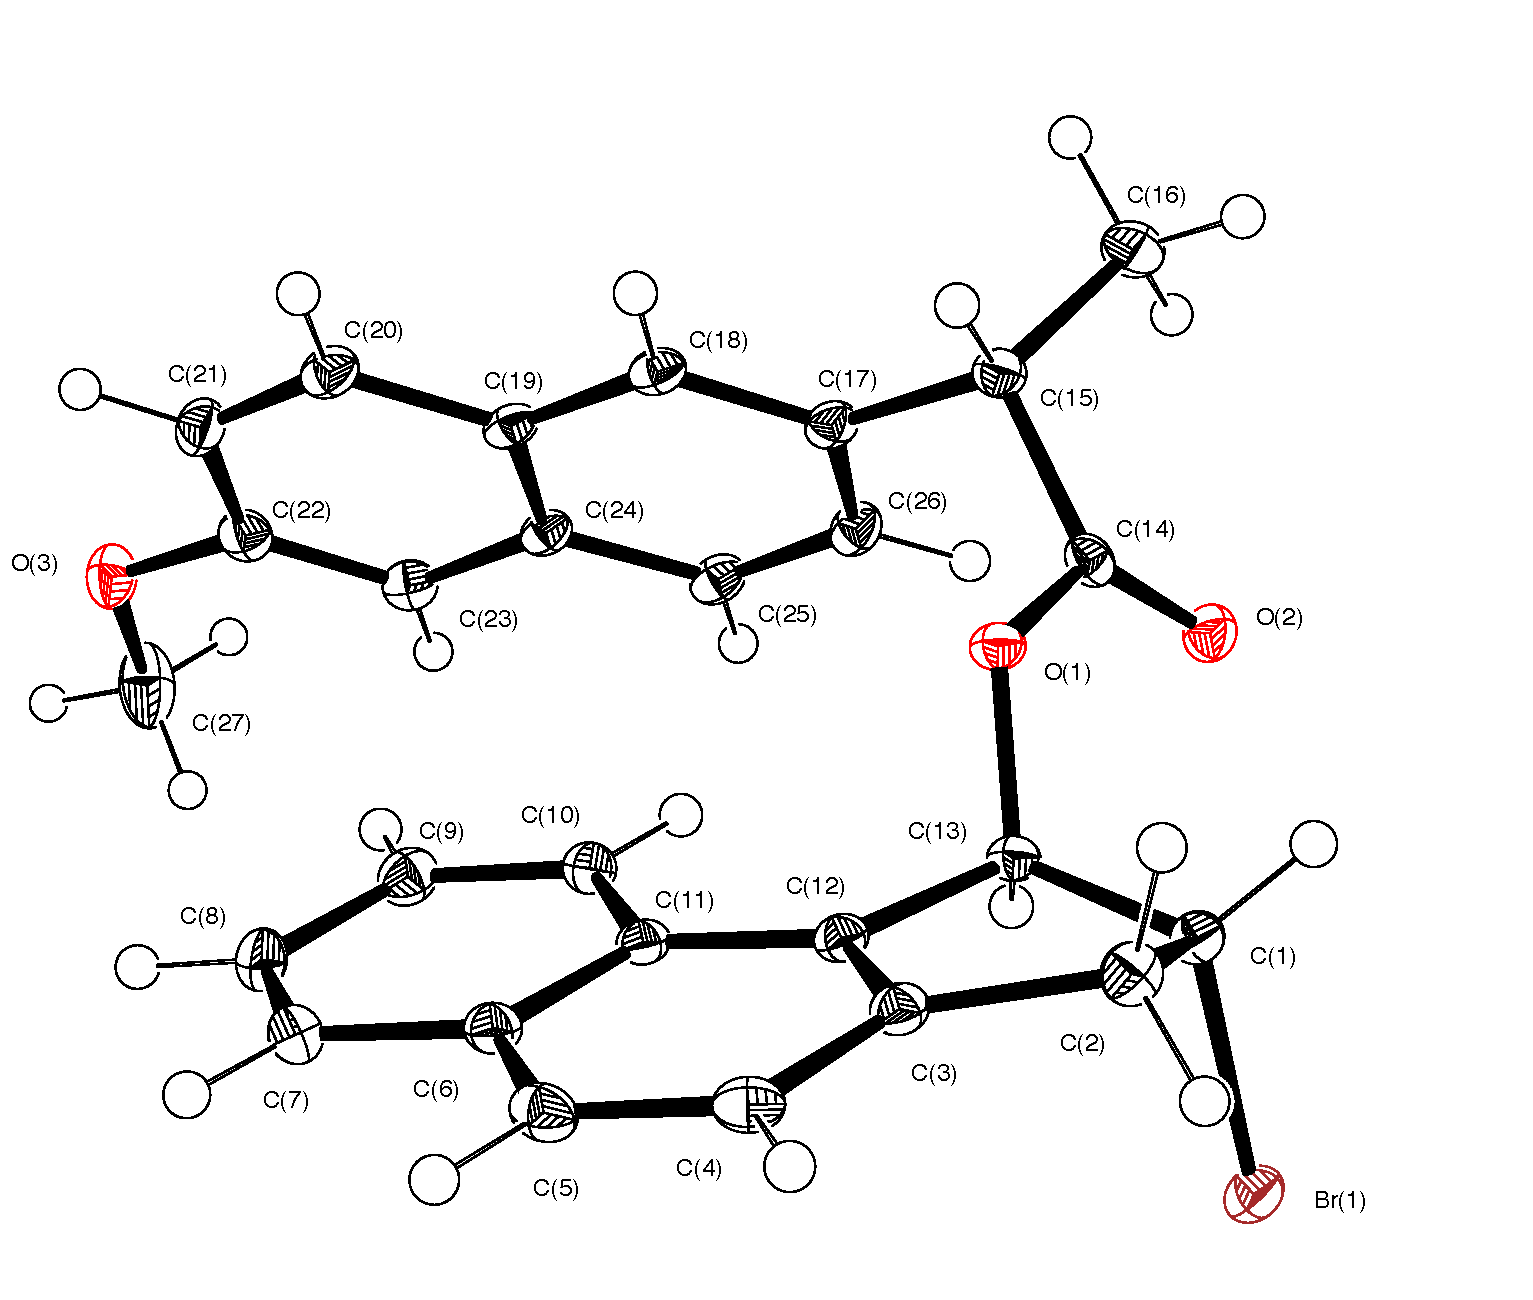
\includegraphics[width=4.5in]{chp_asymmetric/images/xray/xlaag_labelled}
    \begin{textblock}{1}(13,-8.5)
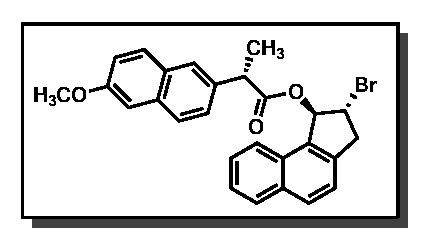
\includegraphics[scale=0.8]{chp_asymmetric/images/xlaag}
\end{textblock}
  \caption{ORTEP drawing of ketone \ref{cmp:xlaag} shown at 50\% probability }
\end{figure}
\pagebreak
\begin{table}[h]
\centering
\caption{Crystal data and structure refinement for \ref{cmp:xlaag}} 
\begin{tabular}{ll} 
\toprule
Empirical formula& 	C$_{27}$H$_{23}$BrO$_3$ \\
Formula weight&	475.36 \\
Temperature &	100(2) K \\
Wavelength& 	0.71073 \AA  \\
Crystal system& 	Orthorhombic \\
Space group& 	P2(1)2(1)2(1) \\
Unit cell dimensions&	a = 6.1357(3) \AA\ $\alpha$ = 90$^\circ$. \\
	&b = 10.2342(5) \AA\	$\beta$ = 90$^\circ$. \\
	&c = 33.8898(17) \AA\	$\gamma$ = 90$^\circ$. \\
Volume&	2128.08(18) \AA$^3$ \\
Z&	4 \\
Density (calculated)&	1.484 Mg/m$^3$ \\
Absorption coefficient&	1.959 mm$^{-1}$ \\
F(000) &	976 \\
Crystal size &	0.18 x 0.15 x 0.10 mm$^3$ \\
Theta range for data collection &	2.08 to 28.34$^\circ$. \\
Index ranges &	$-$8$<=$h$<=$6, $-$13$<=$k$<=$13, $-$45$<=$l$<=$45 \\
Reflections collected &	53379 \\
Independent reflections &	5206 [R(int) = 0.0212] \\
Completeness to theta = 28.34$^\circ$ &	99.7\% \\ 
Absorption correction&	Semi-empirical from equivalents \\
Max. and min. transmission &	0.8282 and 0.7194 \\
Refinement method	&Full-matrix least-squares on F$^2$ \\
Data / restraints / parameters &	 5206 / 0 / 280 \\
Goodness-of-fit on F$^2$ & 	1.125 \\
Final R indices [I$>$2sigma(I)] &	R1 = 0.0195, wR2 = 0.0502 \\
R indices (all data) &	R1 = 0.0199, wR2 = 0.0504 \\
Absolute structure parameter &	0.020(5) \\
Extinction coefficient	& na \\
Largest diff. peak and hole &	0.370 and $-$0.469 e.\AA$^{-3}$ \\
\bottomrule
\end{tabular}
\end{table}

\twocolumn
\begin{table}[h]
\centering
\caption{Atomic coordinates (x 10$^4$) and equivalent isotropic displacement parameters (\AA$^2$x
10$^3$) for \ref{cmp:xlaag}}
{\footnotesize
\begin{tabular}{lcccc} 
\\
\toprule
& x & y & z & U(eq) \\
\midrule
Br(1)&1514(1)&5925(1)&7835(1)&17(1)\\
O(1)&609(2)&7812(1)&6770(1)&14(1)\\
O(2)&3612(2)&8785(1)&7017(1)&18(1)\\
O(3)&6160(2)&4085(1)&4788(1)&22(1)\\
C(1)&$-$34(3)&7079(1)&7462(1)&15(1)\\
C(2)&$-$2447(3)&6689(2)&7454(1)&16(1)\\
C(3)&$-$2478(2)&5627(1)&7145(1)&14(1)\\
C(4)&$-$4106(2)&4675(1)&7076(1)&16(1)\\
C(5)&$-$3846(3)&3825(1)&6768(1)&17(1)\\
C(6)&$-$1993(2)&3881(1)&6517(1)&15(1)\\
C(7)&$-$1742(3)&3009(1)&6194(1)&18(1)\\
C(8)&51(3)&3079(2)&5955(1)&19(1)\\
C(9)&1673(3)&4031(2)&6020(1)&18(1)\\
C(10)&1494(3)&4883(1)&6332(1)&15(1)\\
C(11)&$-$329(3)&4824(1)&6589(1)&13(1)\\
C(12)&$-$636(3)&5672(1)&6915(1)&13(1)\\
C(13)&864(2)&6741(1)&7051(1)&13(1)\\
C(14)&2279(3)&8670(1)&6759(1)&14(1)\\
C(15)&2365(3)&9343(1)&6359(1)&15(1)\\
C(16)&3555(3)&10647(1)&6381(1)&21(1)\\
C(17)&3479(3)&8364(1)&6085(1)&15(1)\\
C(18)&2446(3)&7916(1)&5752(1)&15(1)\\
C(19)&3421(3)&6957(1)&5507(1)&14(1)\\
C(20)&2381(3)&6489(2)&5161(1)&17(1)\\
C(21)&3346(3)&5556(1)&4932(1)&19(1)\\
C(22)&5400(3)&5025(2)&5041(1)&18(1)\\
C(23)&6463(3)&5456(1)&5372(1)&17(1)\\
C(24)&5498(3)&6444(1)&5610(1)&14(1)\\
C(25)&6554(3)&6935(1)&5951(1)&17(1)\\
C(26)&5578(3)&7873(2)&6181(1)&17(1)\\
C(27)&8127(3)&3441(2)&4898(1)&33(1)\\
\bottomrule
\end{tabular}
}
\end{table} 

\begin{center}
\tablefirsthead{%
\toprule}
\tablehead{%
\multicolumn{2}{c}{\footnotesize \textbf{Table \thetable} continued\ldots} \\
\toprule
}
\tabletail{%
%\midrule
\multicolumn{2}{c}{\small \ldots}\\
}
\tablelasttail{\bottomrule}
\topcaption{Bond lengths (\AA) and angles (${^\circ}$) for \ref{cmp:xlaag}}
{\footnotesize \singlespacing
\begin{supertabular}{p{1.5in}c}
Br(1)-C(1) &1.9736(15)\\
O(1)-C(14) &1.3507(18)\\
O(1)-C(13) &1.4615(16)\\
O(2)-C(14) &1.2024(19)\\
O(3)-C(22) &1.3700(19)\\
O(3)-C(27) &1.425(2)\\
C(1)-C(2) &1.533(2)\\
C(1)-C(13) &1.535(2)\\
C(1)-H(1A) &1\\
C(2)-C(3) &1.510(2)\\
C(2)-H(2A) &0.99\\
C(2)-H(2B) &0.99\\
C(3)-C(12) &1.373(2)\\
C(3)-C(4) &1.415(2)\\
C(4)-C(5) &1.367(2)\\
C(4)-H(4A) &0.95\\
C(5)-C(6) &1.421(2)\\
C(5)-H(5A) &0.95\\
C(6)-C(7) &1.419(2)\\
C(6)-C(11) &1.426(2)\\
C(7)-C(8) &1.369(2)\\
C(7)-H(7A) &0.95\\
C(8)-C(9) &1.411(2)\\
C(8)-H(8A) &0.95\\
C(9)-C(10) &1.3741(19)\\
C(9)-H(9A) &0.95\\
C(10)-C(11) &1.419(2)\\
C(10)-H(10A) &0.95\\
C(11)-C(12) &1.4173(19)\\
C(12)-C(13) &1.502(2)\\
C(13)-H(13A) &1\\
C(14)-C(15) &1.521(2)\\
C(15)-C(16) &1.523(2)\\
C(15)-C(17) &1.527(2)\\
C(15)-H(15A) &1\\
C(16)-H(16A) &0.98\\
C(16)-H(16B) &0.98\\
C(16)-H(16C) &0.98\\
C(17)-C(18) &1.374(2)\\
C(17)-C(26) &1.420(2)\\
C(18)-C(19) &1.418(2)\\
C(18)-H(18A) &0.95\\
C(19)-C(20) &1.420(2)\\
C(19)-C(24) &1.422(2)\\
C(20)-C(21) &1.364(2)\\
C(20)-H(20A) &0.95\\
C(21)-C(22) &1.421(2)\\
C(21)-H(21A) &0.95\\
C(22)-C(23) &1.371(2)\\
C(23)-C(24) &1.423(2)\\
C(23)-H(23A) &0.95\\
C(24)-C(25) &1.417(2)\\
C(25)-C(26) &1.373(2)\\
C(25)-H(25A) &0.95\\
C(26)-H(26A) &0.95\\
C(27)-H(27A) &0.98\\
C(27)-H(27B) &0.98\\
C(27)-H(27C) &0.98\\
C(14)-O(1)-C(13)&115.12(11)\\
C(22)-O(3)-C(27)&116.71(13)\\
C(2)-C(1)-C(13)&105.81(12)\\
C(2)-C(1)-Br(1)&108.65(10)\\
C(13)-C(1)-Br(1)&105.81(10)\\
C(2)-C(1)-H(1A)&112.1\\
C(13)-C(1)-H(1A)&112.1\\
Br(1)-C(1)-H(1A)&112.1\\
C(3)-C(2)-C(1)&102.20(12)\\
C(3)-C(2)-H(2A)&111.3\\
C(1)-C(2)-H(2A)&111.3\\
C(3)-C(2)-H(2B)&111.3\\
C(1)-C(2)-H(2B)&111.3\\
H(2A)-C(2)-H(2B)&109.2\\
C(12)-C(3)-C(4)&120.64(13)\\
C(12)-C(3)-C(2)&111.02(13)\\
C(4)-C(3)-C(2)&128.34(14)\\
C(5)-C(4)-C(3)&118.85(14)\\
C(5)-C(4)-H(4A)&120.6\\
C(3)-C(4)-H(4A)&120.6\\
C(4)-C(5)-C(6)&121.63(14)\\
C(4)-C(5)-H(5A)&119.2\\
C(6)-C(5)-H(5A)&119.2\\
C(7)-C(6)-C(5)&121.50(14)\\
C(7)-C(6)-C(11)&118.70(14)\\
C(5)-C(6)-C(11)&119.80(13)\\
C(8)-C(7)-C(6)&120.74(15)\\
C(8)-C(7)-H(7A)&119.6\\
C(6)-C(7)-H(7A)&119.6\\
C(7)-C(8)-C(9)&120.59(14)\\
C(7)-C(8)-H(8A)&119.7\\
C(9)-C(8)-H(8A)&119.7\\
C(10)-C(9)-C(8)&120.24(15)\\
C(10)-C(9)-H(9A)&119.9\\
C(8)-C(9)-H(9A)&119.9\\
C(9)-C(10)-C(11)&120.52(15)\\
C(9)-C(10)-H(10A)&119.7\\
C(11)-C(10)-H(10A)&119.7\\
C(12)-C(11)-C(10)&123.85(13)\\
C(12)-C(11)-C(6)&116.95(13)\\
C(10)-C(11)-C(6)&119.18(13)\\
C(3)-C(12)-C(11)&122.07(13)\\
C(3)-C(12)-C(13)&110.76(12)\\
C(11)-C(12)-C(13)&127.14(14)\\
O(1)-C(13)-C(12)&106.24(11)\\
O(1)-C(13)-C(1)&112.56(11)\\
C(12)-C(13)-C(1)&102.85(12)\\
O(1)-C(13)-H(13A)&111.6\\
C(12)-C(13)-H(13A)&111.6\\
C(1)-C(13)-H(13A)&111.6\\
O(2)-C(14)-O(1)&124.00(13)\\
O(2)-C(14)-C(15)&125.46(14)\\
O(1)-C(14)-C(15)&110.20(12)\\
C(14)-C(15)-C(16)&111.65(12)\\
C(14)-C(15)-C(17)&105.06(11)\\
C(16)-C(15)-C(17)&112.98(13)\\
C(14)-C(15)-H(15A)&109\\
C(16)-C(15)-H(15A)&109\\
C(17)-C(15)-H(15A)&109\\
C(15)-C(16)-H(16A)&109.5\\
C(15)-C(16)-H(16B)&109.5\\
H(16A)-C(16)-H(16B)&109.5\\
C(15)-C(16)-H(16C)&109.5\\
H(16A)-C(16)-H(16C)&109.5\\
H(16B)-C(16)-H(16C)&109.5\\
C(18)-C(17)-C(26)&119.19(14)\\
C(18)-C(17)-C(15)&120.80(15)\\
C(26)-C(17)-C(15)&119.98(13)\\
C(17)-C(18)-C(19)&121.17(15)\\
C(17)-C(18)-H(18A)&119.4\\
C(19)-C(18)-H(18A)&119.4\\
C(18)-C(19)-C(20)&121.88(15)\\
C(18)-C(19)-C(24)&119.33(13)\\
C(20)-C(19)-C(24)&118.79(14)\\
C(21)-C(20)-C(19)&120.69(15)\\
C(21)-C(20)-H(20A)&119.7\\
C(19)-C(20)-H(20A)&119.7\\
C(20)-C(21)-C(22)&120.37(14)\\
C(20)-C(21)-H(21A)&119.8\\
C(22)-C(21)-H(21A)&119.8\\
O(3)-C(22)-C(23)&125.18(16)\\
O(3)-C(22)-C(21)&114.09(14)\\
C(23)-C(22)-C(21)&120.73(15)\\
C(22)-C(23)-C(24)&119.68(16)\\
C(22)-C(23)-H(23A)&120.2\\
C(24)-C(23)-H(23A)&120.2\\
C(25)-C(24)-C(19)&118.66(14)\\
C(25)-C(24)-C(23)&121.63(15)\\
C(19)-C(24)-C(23)&119.71(14)\\
C(26)-C(25)-C(24)&120.69(15)\\
C(26)-C(25)-H(25A)&119.7\\
C(24)-C(25)-H(25A)&119.7\\
C(25)-C(26)-C(17)&120.92(14)\\
C(25)-C(26)-H(26A)&119.5\\
C(17)-C(26)-H(26A)&119.5\\
O(3)-C(27)-H(27A)&109.5\\
O(3)-C(27)-H(27B)&109.5\\
H(27A)-C(27)-H(27B)&109.5\\
O(3)-C(27)-H(27C)&109.5\\
H(27A)-C(27)-H(27C)&109.5\\
H(27B)-C(27)-H(27C)&109.5\\
\end{supertabular}
}
\end{center}

\begin{center}
\tablefirsthead{%
\toprule
&x&y&z&U(eq) \\
\midrule}
\tablehead{%
\multicolumn{5}{c}{\footnotesize \textbf{Table \thetable} continued\ldots} \\
\toprule
&x&y&z&U(eq) \\
\midrule
}
\tabletail{%
%\midrule
\multicolumn{5}{c}{\small \ldots}\\
}
\tablelasttail{\bottomrule}
\topcaption{Hydrogen coordinates (x 10$^4$) and isotropic displacement parameters (\AA$^2$x 10$^3$)
for \ref{cmp:xlaag}} {\footnotesize \singlespacing
\begin{supertabular}{lcccc}
H(1A)&169&8023&7528&17\\
H(2A)&$-$2929&6355&7714&19\\
H(2B)&$-$3382&7435&7377&19\\
H(4A)&$-$5358&4628&7240&19\\
H(5A)&$-$4931&3182&6721&20\\
H(7A)&$-$2830&2370&6144&22\\
H(8A)&205&2480&5742&23\\
H(9A)&2893&4084&5849&22\\
H(10A)&2600&5516&6376&18\\
H(13A)&2410&6435&7065&15\\
H(15A)&843&9497&6264&18\\
H(16A)&2768&11236&6559&31\\
H(16B)&3628&11037&6118&31\\
H(16C)&5035&10507&6482&31\\
H(18A)&1054&8255&5684&18\\
H(20A)&999&6828&5087&21\\
H(21A)&2642&5261&4699&22\\
H(23A)&7837&5096&5442&21\\
H(25A)&7953&6612&6022&20\\
H(26A)&6318&8198&6407&20\\
H(27A)&8508&2793&4697&49\\
H(27B)&7923&3003&5152&49\\
H(27C)&9303&4085&4920&49\\
\end{supertabular}
}
\end{center}

\pagebreak
\begin{center}
\tablefirsthead{%
\toprule}
\tablehead{%
\multicolumn{2}{c}{\footnotesize \textbf{Table \thetable} continued\ldots} \\
\toprule
}
\tabletail{%
%\midrule
\multicolumn{2}{c}{\small \ldots}\\
}
\tablelasttail{\bottomrule}
\topcaption{Torsion angles ($^{\circ}$) for \ref{cmp:xlaag}}
{\footnotesize \singlespacing
\begin{supertabular}{p{1.5in}c}
C(13)-C(1)-C(2)-C(3)&26.23(14)\\
Br(1)-C(1)-C(2)-C(3)&$-$87.00(12)\\
C(1)-C(2)-C(3)-C(12)&$-$17.68(16)\\
C(1)-C(2)-C(3)-C(4)&162.81(14)\\
C(12)-C(3)-C(4)-C(5)&$-$1.9(2)\\
C(2)-C(3)-C(4)-C(5)&177.55(14)\\
C(3)-C(4)-C(5)-C(6)&$-$0.3(2)\\
C(4)-C(5)-C(6)-C(7)&$-$179.09(14)\\
C(4)-C(5)-C(6)-C(11)&1.3(2)\\
C(5)-C(6)-C(7)-C(8)&179.80(14)\\
C(11)-C(6)-C(7)-C(8)&$-$0.6(2)\\
C(6)-C(7)-C(8)-C(9)&$-$0.9(2)\\
C(7)-C(8)-C(9)-C(10)&1.5(2)\\
C(8)-C(9)-C(10)-C(11)&$-$0.6(2)\\
C(9)-C(10)-C(11)-C(12)&$-$179.58(14)\\
C(9)-C(10)-C(11)-C(6)&$-$0.9(2)\\
C(7)-C(6)-C(11)-C(12)&$-$179.73(13)\\
C(5)-C(6)-C(11)-C(12)&$-$0.1(2)\\
C(7)-C(6)-C(11)-C(10)&1.5(2)\\
C(5)-C(6)-C(11)-C(10)&$-$178.94(13)\\
C(4)-C(3)-C(12)-C(11)&3.2(2)\\
C(2)-C(3)-C(12)-C(11)&$-$176.36(13)\\
C(4)-C(3)-C(12)-C(13)&$-$178.73(13)\\
C(2)-C(3)-C(12)-C(13)&1.72(16)\\
C(10)-C(11)-C(12)-C(3)&176.64(13)\\
C(6)-C(11)-C(12)-C(3)&$-$2.1(2)\\
C(10)-C(11)-C(12)-C(13)&$-$1.1(2)\\
C(6)-C(11)-C(12)-C(13)&$-$179.86(13)\\
C(14)-O(1)-C(13)-C(12)&$-$159.00(12)\\
C(14)-O(1)-C(13)-C(1)&89.17(15)\\
C(3)-C(12)-C(13)-O(1)&$-$103.41(13)\\
C(11)-C(12)-C(13)-O(1)&74.55(17)\\
C(3)-C(12)-C(13)-C(1)&15.03(15)\\
C(11)-C(12)-C(13)-C(1)&$-$167.01(14)\\
C(2)-C(1)-C(13)-O(1)&88.44(14)\\
Br(1)-C(1)-C(13)-O(1)&$-$156.36(9)\\
C(2)-C(1)-C(13)-C(12)&$-$25.48(14)\\
Br(1)-C(1)-C(13)-C(12)&89.72(11)\\
C(13)-O(1)-C(14)-O(2)&$-$18.5(2)\\
C(13)-O(1)-C(14)-C(15)&155.10(12)\\
O(2)-C(14)-C(15)-C(16)&$-$29.1(2)\\
O(1)-C(14)-C(15)-C(16)&157.37(13)\\
O(2)-C(14)-C(15)-C(17)&93.68(17)\\
O(1)-C(14)-C(15)-C(17)&$-$79.82(15)\\
C(14)-C(15)-C(17)-C(18)&121.44(14)\\
C(16)-C(15)-C(17)-C(18)&$-$116.62(16)\\
C(14)-C(15)-C(17)-C(26)&$-$56.50(17)\\
C(16)-C(15)-C(17)-C(26)&65.44(17)\\
C(26)-C(17)-C(18)-C(19)&1.2(2)\\
C(15)-C(17)-C(18)-C(19)&$-$176.72(13)\\
C(17)-C(18)-C(19)-C(20)&$-$179.67(14)\\
C(17)-C(18)-C(19)-C(24)&0.5(2)\\
C(18)-C(19)-C(20)-C(21)&$-$179.37(14)\\
C(24)-C(19)-C(20)-C(21)&0.5(2)\\
C(19)-C(20)-C(21)-C(22)&0.9(2)\\
C(27)-O(3)-C(22)-C(23)&5.1(2)\\
C(27)-O(3)-C(22)-C(21)&$-$175.16(15)\\
C(20)-C(21)-C(22)-O(3)&179.08(14)\\
C(20)-C(21)-C(22)-C(23)&$-$1.2(2)\\
O(3)-C(22)-C(23)-C(24)&179.80(14)\\
C(21)-C(22)-C(23)-C(24)&0.1(2)\\
C(18)-C(19)-C(24)-C(25)&$-$1.6(2)\\
C(20)-C(19)-C(24)-C(25)&178.56(14)\\
C(18)-C(19)-C(24)-C(23)&178.31(13)\\
C(20)-C(19)-C(24)-C(23)&$-$1.6(2)\\
C(22)-C(23)-C(24)-C(25)&$-$178.87(14)\\
C(22)-C(23)-C(24)-C(19)&1.3(2)\\
C(19)-C(24)-C(25)-C(26)&1.0(2)\\
C(23)-C(24)-C(25)-C(26)&$-$178.89(14)\\
C(24)-C(25)-C(26)-C(17)&0.7(2)\\
C(18)-C(17)-C(26)-C(25)&$-$1.8(2)\\
C(15)-C(17)-C(26)-C(25)&176.13(14)\\
\end{supertabular}
}
\end{center}

\onecolumn
\begin{table}[h]
\centering
\caption{Anisotropic displacement parameters (\AA$^2$x 10$^3$) for \ref{cmp:xlaag}} 
\footnotesize
\begin{tabular}{p{1in}cccccc} 
\toprule
& U$^{11}$ & U$^{22}$ & U$^{33}$ & U$^{23}$ & U$^{13}$ & U$^{12}$ \\
\midrule
Br(1)&18(1) &20(1)&13(1) &2(1)&$-$2(1) &$-$1(1)\\
O(1)&14(1) &13(1)&14(1) &3(1)&$-$1(1) &$-$1(1)\\
O(2)&19(1) &18(1)&16(1) &0(1)&$-$2(1) &$-$4(1)\\
O(3)&22(1) &23(1)&21(1) &$-$7(1)&$-$1(1) &2(1)\\
C(1)&17(1) &14(1)&13(1) &0(1)&$-$1(1) &1(1)\\
C(2)&14(1) &18(1)&16(1) &0(1)&2(1) &1(1)\\
C(3)&14(1) &14(1)&13(1) &2(1)&$-$1(1) &2(1)\\
C(4)&13(1) &16(1)&18(1) &4(1)&1(1) &1(1)\\
C(5)&14(1) &15(1)&22(1) &3(1)&$-$3(1) &$-$3(1)\\
C(6)&15(1) &13(1)&15(1) &2(1)&$-$2(1) &$-$1(1)\\
C(7)&22(1) &15(1)&17(1) &0(1)&$-$2(1) &$-$3(1)\\
C(8)&25(1) &18(1)&14(1) &$-$4(1)&$-$1(1) &1(1)\\
C(9)&19(1) &21(1)&16(1) &1(1)&2(1) &2(1)\\
C(10)&15(1) &14(1)&15(1) &1(1)&0(1) &0(1)\\
C(11)&14(1) &12(1)&12(1) &2(1)&$-$2(1) &0(1)\\
C(12)&13(1) &14(1)&12(1) &2(1)&$-$2(1) &0(1)\\
C(13)&14(1) &12(1)&13(1) &2(1)&0(1) &$-$1(1)\\
C(14)&15(1) &12(1)&16(1) &$-$2(1)&2(1) &1(1)\\
C(15)&15(1) &13(1)&16(1) &1(1)&$-$2(1) &$-$1(1)\\
C(16)&24(1) &16(1)&22(1) &3(1)&0(1) &$-$6(1)\\
C(17)&16(1) &16(1)&12(1) &3(1)&2(1) &$-$2(1)\\
C(18)&12(1) &17(1)&15(1) &4(1)&$-$1(1) &$-$1(1)\\
C(19)&14(1) &17(1)&12(1) &4(1)&0(1) &$-$2(1)\\
C(20)&15(1) &20(1)&17(1) &4(1)&$-$3(1) &$-$2(1)\\
C(21)&19(1) &22(1)&15(1) &0(1)&$-$3(1) &$-$4(1)\\
C(22)&19(1) &17(1)&17(1) &1(1)&3(1) &$-$3(1)\\
C(23)&15(1) &19(1)&18(1) &2(1)&1(1) &0(1)\\
C(24)&14(1) &17(1)&12(1) &3(1)&1(1) &$-$2(1)\\
C(25)&13(1) &21(1)&16(1) &3(1)&$-$2(1) &$-$1(1)\\
C(26)&15(1) &20(1)&15(1) &1(1)&$-$2(1) &$-$3(1)\\
C(27)&22(1) &37(1)&39(1) &$-$18(1)&$-$4(1) &7(1)\\
\bottomrule
\end{tabular}
\end{table}
{ \footnotesize
The anisotropic displacement factor exponent takes the form: 
$-2\pi^2\left[ h^2a*^2U^{11} + ... + 2 h k a* b* U^{12} \right]$ }

\pagebreak
%%%%%%%%%%% End of X-Ray Data for xlaag %%%%%%%%%%%%%%%%%%%%


%%%%%%%%%%% Begin  X-Ray Data for xlaak %%%%%%%%%%%%%%%%%%%%
\subsection{Structural Data for  \ref{cmp:xlaak} Copper Chloride Complex}
Bis(oxazoline) ligand \ref{cmp:xlaak} (25.0 mg, 0.054 mmol, 1.00
equiv) was dissolved in 2 mL of CH$_2$Cl$_2$. CuCl$_2$ (25.0 mg, 0.186 mmol,
3.44 equiv) was added as a solid and the suspension was stirred for 1 hour at room temperature. The suspension was filtered through a cotton plug into
a 1 dram glass shell vial that was placed into a 25 mL scintillation vial
containing 5 mL of pentane. The scintillation vial was sealed with a screw cap for 1 week,
after which time suitable orange X-ray quality crystals of
\ce{CuCl2.}\ref{cmp:xlaak} were obtained. The structure of \ce{CuCl2.}\ref{cmp:xlaak} has been
deposited with the Cambridge Crystallographic Data Centre (CCDC \#845000).
\vspace{-45pt}
\begin{figure}[h]
  \centering
  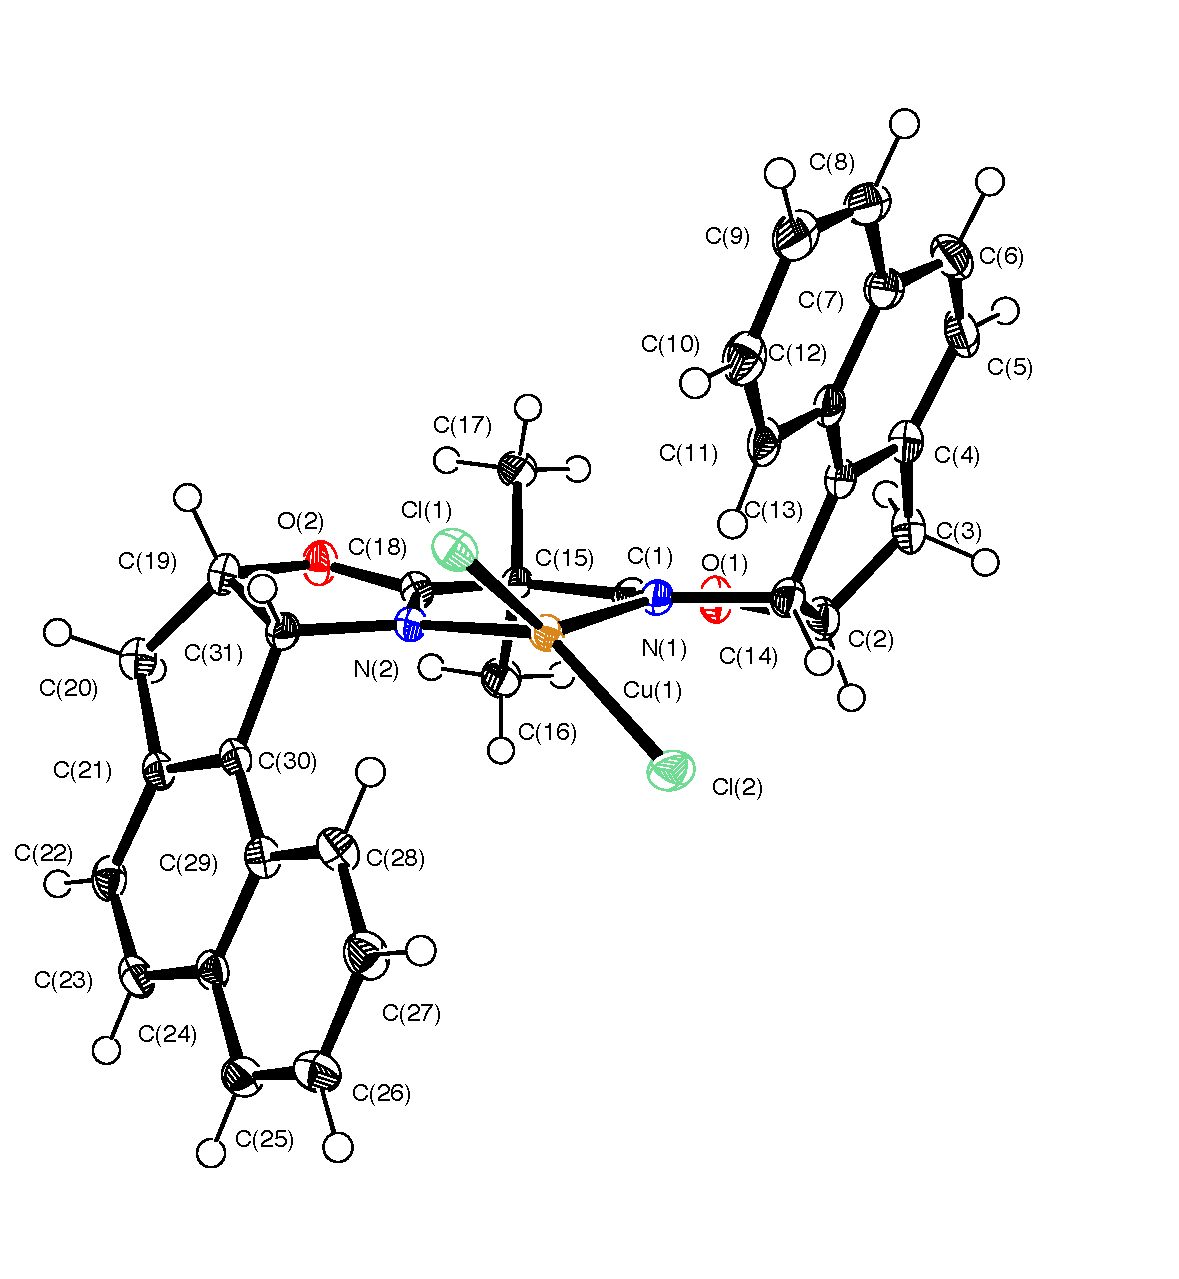
\includegraphics[width=5.0in]{chp_asymmetric/images/xray/boxcomplex_labelled}
  \caption{ORTEP drawing of \ce{CuCl2.}\ref{cmp:xlaak} shown at 50\% probability }
\end{figure}
\pagebreak
\begin{table}[h]
\centering
\caption{Crystal data and structure refinement for \ce{CuCl2.}\ref{cmp:xlaak}} 
\begin{tabular}{ll} 
\toprule
Empirical formula& 	C$_{32}$H$_{28}$Cl$_4$CuN$_2$O$_2$ (contains CH$_2$Cl$_2$)\\ 
Formula weight&	677.90 \\
Temperature &	100(2) K \\
Wavelength& 	0.71073 \AA  \\
Crystal system& 	Triclinic\\
Space group& 	P 1 \\
Unit cell dimensions&	a = 13.3742(5) \AA\ 	$\alpha$ = 88.632(2)$^\circ$. \\
	&b = 18.7820(7) \AA\ 	$\beta$ = 77.873(2)$^\circ$. \\
	&c = 25.5722(10) \AA\ 	$\gamma$ = 74.830(2)$^\circ$. \\
Volume&	6058.1(4) \AA$^3$ \\
Z&	8 \\
Density (calculated)&	1.487 Mg/m$^3$ \\
Absorption coefficient&	1.107 mm$^{-1}$ \\
F(000) &	2776 \\
Crystal size &	0.12 x 0.10 x 0.07 mm$^3$ \\
Theta range for data collection &	1.12 to 28.70$^\circ$. \\
Index ranges &	$-$17$<=$h$<=$17, $-$25$<=$k$<=$25, $-$34$<=$l$<=$34 \\
Reflections collected &	220519 \\
Independent reflections &	58427 [R(int) = 0.0240] \\
Completeness to theta = 28.70$^\circ$ &	97.8 \% \\ 
Absorption correction&	Semi-empirical from equivalents \\
Max. and min. transmission &	0.9265 and 0.8786 \\
Refinement method	&Full-matrix least-squares on F$^2$ \\
Data / restraints / parameters &	 58427 / 0 / 2950 \\
Goodness-of-fit on F$^2$ & 	1.029 \\
Final R indices [I$>$2sigma(I)] &	R1 = 0.0489, wR2 = 0.1324 \\
R indices (all data) &	R1 = 0.0536, wR2 = 0.1371 \\
Absolute structure parameter &	0.018(4) \\
Extinction coefficient	& na \\
Largest diff. peak and hole &	2.523 and $-$1.276 e.\AA$^{-3}$ \\
\bottomrule
\end{tabular}
\end{table}
\pagebreak


\twocolumn
\begin{center}
\tablefirsthead{%
\toprule
&x&y&z&U(eq) \\
\midrule}
\tablehead{%
\multicolumn{5}{c}{\footnotesize \textbf{Table \thetable} continued\ldots} \\
\toprule
&x&y&z&U(eq) \\
\midrule
}
\tabletail{%
%\midrule
\multicolumn{5}{c}{\small \ldots}\\
}
\tablelasttail{\bottomrule}
\topcaption{Atomic coordinates (x 10$^4$) and equivalent isotropic displacement parameters (\AA$^2$x
10$^3$) for \ce{CuCl2.}\ref{cmp:xlaak}} {\footnotesize \singlespacing
\begin{supertabular}{lcccc}
Cu(1)&5923(1)&3980(1)&3895(1)&16(1)\\
Cl(1)&5758(1)&4665(1)&4622(1)&21(1)\\
Cl(2)&7639(1)&3375(1)&3750(1)&25(1)\\
O(1)&5478(2)&3770(1)&2367(1)&23(1)\\
O(2)&2868(2)&3874(1)&3954(1)&22(1)\\
N(1)&5899(2)&4040(2)&3124(1)&17(1)\\
N(2)&4505(2)&3794(1)&4070(1)&16(1)\\
C(1)&5211(3)&3870(2)&2901(1)&18(1)\\
C(2)&6575(3)&3810(2)&2190(1)&23(1)\\
C(3)&6647(3)&4372(2)&1754(1)&26(1)\\
C(4)&6676(3)&5049(2)&2049(1)&23(1)\\
C(5)&6614(3)&5757(2)&1839(2)&28(1)\\
C(6)&6651(3)&6318(2)&2157(2)&30(1)\\
C(7)&6756(3)&6200(2)&2693(2)&24(1)\\
C(8)&6752(3)&6788(2)&3033(2)&29(1)\\
C(9)&6847(3)&6667(2)&3553(2)&30(1)\\
C(10)&7008(3)&5950(2)&3753(2)&27(1)\\
C(11)&7034(3)&5363(2)&3428(1)&22(1)\\
C(12)&6868(3)&5479(2)&2903(1)&21(1)\\
C(13)&6785(3)&4914(2)&2567(1)&20(1)\\
C(14)&6805(3)&4122(2)&2692(1)&20(1)\\
C(15)&4121(2)&3798(2)&3139(1)&16(1)\\
C(16)&4004(3)&3036(2)&2973(2)&24(1)\\
C(17)&3327(3)&4425(2)&2926(1)&23(1)\\
C(18)&3878(3)&3832(2)&3742(1)&18(1)\\
C(19)&2727(3)&3895(2)&4538(1)&20(1)\\
C(20)&2285(3)&3253(2)&4762(1)&22(1)\\
C(21)&3232(3)&2691(2)&4885(1)&18(1)\\
C(22)&3269(3)&1969(2)&5048(1)&21(1)\\
C(23)&4188(3)&1518(2)&5143(1)&21(1)\\
C(24)&5102(3)&1787(2)&5109(1)&18(1)\\
C(25)&6059(3)&1333(2)&5218(1)&22(1)\\
C(26)&6917(3)&1597(2)&5197(2)&25(1)\\
C(27)&6876(3)&2338(2)&5066(2)&25(1)\\
C(28)&5967(3)&2793(2)&4952(1)&22(1)\\
C(29)&5067(3)&2529(2)&4958(1)&19(1)\\
C(30)&4108(3)&2964(2)&4826(1)&17(1)\\
C(31)&3878(3)&3745(2)&4617(1)&17(1)\\
Cu(2)&5894(1)&8992(1)&3907(1)&15(1)\\
Cl(3)&7629(1)&8427(1)&3737(1)&23(1)\\
Cl(4)&5738(1)&9662(1)&4641(1)&21(1)\\
O(3)&5346(2)&8809(1)&2396(1)&23(1)\\
O(4)&2833(2)&8869(1)&4007(1)&22(1)\\
N(3)&5825(2)&9064(1)&3141(1)&16(1)\\
N(4)&4488(2)&8786(2)&4100(1)&17(1)\\
C(32)&5128(3)&8894(2)&2928(1)&16(1)\\
C(33)&6437(3)&8855(2)&2201(1)&21(1)\\
C(34)&6478(3)&9420(2)&1765(1)&23(1)\\
C(35)&6476(3)&10105(2)&2060(1)&21(1)\\
C(36)&6369(3)&10819(2)&1848(1)&24(1)\\
C(37)&6407(3)&11386(2)&2166(2)&26(1)\\
C(38)&6564(3)&11258(2)&2696(2)&21(1)\\
C(39)&6565(3)&11845(2)&3034(2)&26(1)\\
C(40)&6664(3)&11727(2)&3554(2)&27(1)\\
C(41)&6824(3)&11013(2)&3755(2)&23(1)\\
C(42)&6866(3)&10423(2)&3431(1)&20(1)\\
C(43)&6690(2)&10537(2)&2906(1)&17(1)\\
C(44)&6616(2)&9972(2)&2570(1)&17(1)\\
C(45)&6692(3)&9165(2)&2696(1)&18(1)\\
C(46)&4062(3)&8781(2)&3183(1)&16(1)\\
C(47)&4032(3)&7988(2)&3042(2)&26(1)\\
C(48)&3209(3)&9353(2)&2964(1)&24(1)\\
C(49)&3835(3)&8830(2)&3785(1)&19(1)\\
C(50)&2716(3)&8889(2)&4592(1)&20(1)\\
C(51)&2280(3)&8248(2)&4820(1)&23(1)\\
C(52)&3231(3)&7683(2)&4927(1)&20(1)\\
C(53)&3271(3)&6957(2)&5096(1)&21(1)\\
C(54)&4195(3)&6503(2)&5179(1)&21(1)\\
C(55)&5127(3)&6766(2)&5122(1)&19(1)\\
C(56)&6088(3)&6304(2)&5223(1)&23(1)\\
C(57)&6959(3)&6559(2)&5182(2)&28(1)\\
C(58)&6923(3)&7303(2)&5048(1)&25(1)\\
C(59)&6002(3)&7757(2)&4942(1)&23(1)\\
C(60)&5091(3)&7504(2)&4966(1)&18(1)\\
C(61)&4122(3)&7946(2)&4853(1)&17(1)\\
C(62)&3889(3)&8728(2)&4654(1)&18(1)\\
Cu(3)&632(1)&7628(1)&7046(1)&12(1)\\
Cl(5)&1147(1)&8220(1)&6318(1)&19(1)\\
Cl(6)&$-$1074(1)&7793(1)&7024(1)&18(1)\\
O(5)&3478(2)&6256(1)&7250(1)&21(1)\\
O(6)&495(2)&7247(1)&8652(1)&20(1)\\
N(5)&1988(2)&6861(1)&6999(1)&14(1)\\
N(6)&395(2)&7676(1)&7837(1)&14(1)\\
C(63)&2464(2)&6654(2)&7382(1)&14(1)\\
C(64)&3802(3)&6235(2)&6666(1)&19(1)\\
C(65)&4264(3)&5445(2)&6447(1)&20(1)\\
C(66)&3386(3)&5279(2)&6232(1)&17(1)\\
C(67)&3404(3)&4597(2)&6009(1)&19(1)\\
C(68)&2521(3)&4518(2)&5848(1)&19(1)\\
C(69)&1607(3)&5127(2)&5882(1)&16(1)\\
C(70)&694(3)&5046(2)&5720(1)&20(1)\\
C(71)&$-$172(3)&5641(2)&5741(1)&22(1)\\
C(72)&$-$144(3)&6343(2)&5904(1)&22(1)\\
C(73)&738(3)&6439(2)&6059(1)&19(1)\\
C(74)&1627(2)&5831(2)&6070(1)&15(1)\\
C(75)&2533(2)&5884(2)&6259(1)&15(1)\\
C(76)&2738(2)&6553(2)&6490(1)&15(1)\\
C(77)&2037(2)&6733(2)&7980(1)&15(1)\\
C(78)&2757(3)&7070(2)&8248(1)&20(1)\\
C(79)&2064(3)&5952(2)&8181(2)&22(1)\\
C(80)&932(3)&7240(2)&8129(1)&15(1)\\
C(81)&$-$601(3)&7719(2)&8728(1)&19(1)\\
C(82)&$-$837(3)&8293(2)&9176(1)&23(1)\\
C(83)&$-$670(3)&8975(2)&8884(1)&19(1)\\
C(84)&$-$747(3)&9671(2)&9121(1)&26(1)\\
C(85)&$-$669(3)&10253(2)&8809(2)&25(1)\\
C(86)&$-$501(3)&10182(2)&8242(2)&21(1)\\
C(87)&$-$456(3)&10799(2)&7919(2)&25(1)\\
C(88)&$-$312(3)&10729(2)&7370(2)&26(1)\\
C(89)&$-$243(3)&10041(2)&7135(2)&23(1)\\
C(90)&$-$298(3)&9438(2)&7441(1)&19(1)\\
C(91)&$-$423(2)&9486(2)&8001(1)&15(1)\\
C(92)&$-$516(2)&8887(2)&8343(1)&15(1)\\
C(93)&$-$583(3)&8123(2)&8196(1)&16(1)\\
Cu(4)&632(1)&2654(1)&7045(1)&13(1)\\
Cl(7)&1070(1)&3278(1)&6324(1)&21(1)\\
Cl(8)&$-$1080(1)&2799(1)&7054(1)&19(1)\\
O(7)&3560(2)&1366(1)&7200(1)&20(1)\\
O(8)&611(2)&2220(1)&8635(1)&20(1)\\
N(7)&2022(2)&1923(1)&6972(1)&15(1)\\
N(8)&451(2)&2682(1)&7834(1)&14(1)\\
C(94)&2532(2)&1722(2)&7344(1)&15(1)\\
C(95)&3846(3)&1347(2)&6611(1)&21(1)\\
C(96)&4317(3)&551(2)&6405(1)&22(1)\\
C(97)&3425(3)&356(2)&6218(1)&17(1)\\
C(98)&3435(3)&$-$342(2)&6028(1)&20(1)\\
C(99)&2551(3)&$-$432(2)&5877(1)&20(1)\\
C(100)&1647(3)&170(2)&5885(1)&18(1)\\
C(101)&743(3)&73(2)&5724(1)&22(1)\\
C(102)&$-$120(3)&667(2)&5722(1)&24(1)\\
C(103)&$-$92(3)&1380(2)&5866(1)&24(1)\\
C(104)&773(3)&1493(2)&6024(1)&20(1)\\
C(105)&1659(3)&887(2)&6051(1)&16(1)\\
C(106)&2571(3)&956(2)&6232(1)&15(1)\\
C(107)&2762(2)&1640(2)&6451(1)&17(1)\\
C(108)&2118(2)&1735(2)&7943(1)&15(1)\\
C(109)&2115(3)&935(2)&8088(1)&20(1)\\
C(110)&2845(3)&2011(2)&8243(1)&19(1)\\
C(111)&1018(3)&2238(2)&8111(1)&15(1)\\
C(112)&$-$503(3)&2667(2)&8728(1)&19(1)\\
C(113)&$-$730(3)&3210(2)&9197(1)&21(1)\\
C(114)&$-$580(3)&3908(2)&8930(1)&19(1)\\
C(115)&$-$631(3)&4578(2)&9189(1)&25(1)\\
C(116)&$-$579(3)&5186(2)&8890(2)&25(1)\\
C(117)&$-$449(3)&5159(2)&8327(2)&20(1)\\
C(118)&$-$424(3)&5796(2)&8020(2)&24(1)\\
C(119)&$-$299(3)&5755(2)&7475(2)&27(1)\\
C(120)&$-$213(3)&5084(2)&7213(2)&22(1)\\
C(121)&$-$264(3)&4465(2)&7502(1)&18(1)\\
C(122)&$-$371(2)&4477(2)&8057(1)&16(1)\\
C(123)&$-$454(2)&3858(2)&8382(1)&16(1)\\
C(124)&$-$516(2)&3104(2)&8215(1)&16(1)\\
Cu(5)&5547(1)&7168(1)&8804(1)&20(1)\\
Cl(9)&6562(1)&7958(1)&8780(1)&25(1)\\
Cl(10)&4077(1)&7745(1)&9385(1)&30(1)\\
O(9)&6817(2)&6058(1)&7346(1)&22(1)\\
O(10)&5070(2)&5094(1)&8895(1)&29(1)\\
N(9)&6030(2)&6843(2)&8047(1)&18(1)\\
N(10)&5467(2)&6154(2)&9010(1)&19(1)\\
C(125)&6285(3)&6182(2)&7852(1)&17(1)\\
C(126)&7097(3)&6751(2)&7168(1)&20(1)\\
C(127)&6773(3)&6955(2)&6633(2)&30(1)\\
C(128)&5685(3)&7445(2)&6798(2)&27(1)\\
C(129)&4922(4)&7687(2)&6473(2)&34(1)\\
C(130)&3937(4)&8104(2)&6696(2)&40(1)\\
C(131)&3676(3)&8371(2)&7231(2)&34(1)\\
C(132)&2663(3)&8823(2)&7460(2)&40(1)\\
C(133)&2430(3)&9089(2)&7978(2)&44(1)\\
C(134)&3215(3)&8929(2)&8284(2)&36(1)\\
C(135)&4210(3)&8481(2)&8081(2)&27(1)\\
C(136)&4468(3)&8173(2)&7554(2)&24(1)\\
C(137)&5442(3)&7681(2)&7324(2)&22(1)\\
C(138)&6358(3)&7316(2)&7595(1)&19(1)\\
C(139)&6042(2)&5496(2)&8110(1)&15(1)\\
C(140)&7094(3)&4910(2)&8118(2)&22(1)\\
C(141)&5390(3)&5197(2)&7786(2)&24(1)\\
C(142)&5482(2)&5635(2)&8690(1)&18(1)\\
C(143)&4591(3)&5292(2)&9460(2)&34(1)\\
C(144)&5039(4)&4656(2)&9809(2)&42(1)\\
C(145)&5929(4)&4858(3)&9963(2)&44(1)\\
C(146)&6715(5)&4420(3)&10242(2)&60(2)\\
C(147)&7452(4)&4718(3)&10369(2)&49(1)\\
C(148)&7494(4)&5440(3)&10251(2)&48(1)\\
C(149)&8296(4)&5727(3)&10389(2)&51(1)\\
C(150)&8343(4)&6418(4)&10257(2)&57(2)\\
C(151)&7605(4)&6883(3)&9973(2)&49(1)\\
C(152)&6825(3)&6608(3)&9844(2)&36(1)\\
C(153)&6753(3)&5896(3)&9972(1)&34(1)\\
C(154)&5957(3)&5569(2)&9840(2)&34(1)\\
C(155)&5064(3)&5930(2)&9560(1)&25(1)\\
Cu(6)&5708(1)&2037(1)&8906(1)&21(1)\\
Cl(11)&6857(1)&2719(1)&8901(1)&34(1)\\
Cl(12)&4464(1)&2623(1)&9594(1)&31(1)\\
O(11)&6726(2)&1128(1)&7368(1)&22(1)\\
O(12)&4842(2)&109(1)&8827(1)&23(1)\\
N(11)&6049(2)&1828(2)&8123(1)&18(1)\\
N(12)&5454(2)&1045(2)&9040(1)&19(1)\\
C(156)&6250(2)&1195(2)&7885(1)&17(1)\\
C(157)&7029(3)&1825(2)&7226(1)&23(1)\\
C(158)&6639(3)&2119(2)&6726(2)&31(1)\\
C(159)&5557(3)&2614(2)&6944(2)&28(1)\\
C(160)&4747(4)&2915(2)&6658(2)&34(1)\\
C(161)&3783(3)&3324(2)&6935(2)&34(1)\\
C(162)&3595(3)&3512(2)&7489(2)&31(1)\\
C(163)&2599(3)&3938(2)&7776(2)&41(1)\\
C(164)&2438(3)&4096(2)&8304(2)&40(1)\\
C(165)&3282(3)&3870(2)&8578(2)&34(1)\\
C(166)&4259(3)&3454(2)&8312(2)&28(1)\\
C(167)&4442(3)&3246(2)&7768(2)&28(1)\\
C(168)&5401(3)&2775(2)&7479(2)&22(1)\\
C(169)&6354(3)&2344(2)&7698(1)&21(1)\\
C(170)&6009(2)&494(2)&8108(1)&15(1)\\
C(171)&5422(3)&199(2)&7741(1)&23(1)\\
C(172)&7060(3)&$-$88(2)&8127(1)&21(1)\\
C(173)&5400(2)&605(2)&8676(1)&17(1)\\
C(174)&4344(3)&264(2)&9400(2)&25(1)\\
C(175)&4588(3)&$-$453(2)&9701(2)&31(1)\\
C(176)&5525(3)&$-$405(2)&9906(1)&29(1)\\
C(177)&6138(4)&$-$983(2)&10173(2)&35(1)\\
C(178)&6952(4)&$-$849(2)&10361(2)&37(1)\\
C(179)&7216(3)&$-$170(2)&10304(1)&31(1)\\
C(180)&8044(4)&$-$20(3)&10507(2)&39(1)\\
C(181)&8301(4)&636(3)&10431(2)&35(1)\\
C(182)&7733(4)&1194(3)&10156(2)&42(1)\\
C(183)&6892(3)&1078(2)&9960(2)&33(1)\\
C(184)&6608(3)&410(2)&10028(1)&30(1)\\
C(185)&5753(3)&266(2)&9836(1)&27(1)\\
C(186)&4962(3)&785(2)&9563(1)&23(1)\\
Cu(7)&2279(1)&5962(1)&1977(1)&16(1)\\
Cl(13)&4034(1)&5598(1)&1700(1)&23(1)\\
Cl(14)&2069(1)&7179(1)&1876(1)&23(1)\\
O(13)&1490(2)&4025(1)&1757(1)&26(1)\\
O(14)&$-$610(2)&5976(1)&2956(1)&22(1)\\
N(13)&2028(2)&5062(2)&1696(1)&17(1)\\
N(14)&1021(2)&6057(1)&2572(1)&17(1)\\
C(187)&1360(3)&4715(2)&1927(1)&18(1)\\
C(188)&2489(3)&3825(2)&1354(2)&26(1)\\
C(189)&2278(3)&3529(2)&849(2)&31(1)\\
C(190)&1985(3)&4206(2)&540(2)&26(1)\\
C(191)&1486(3)&4289(2)&102(2)&33(1)\\
C(192)&1292(3)&4950(2)&$-$140(2)&33(1)\\
C(193)&1610(3)&5556(2)&31(1)&24(1)\\
C(194)&1435(3)&6245(2)&$-$225(2)&31(1)\\
C(195)&1804(3)&6801(2)&$-$78(2)&29(1)\\
C(196)&2365(3)&6706(2)&336(2)&24(1)\\
C(197)&2514(3)&6063(2)&610(1)&18(1)\\
C(198)&2131(3)&5474(2)&465(1)&18(1)\\
C(199)&2268(3)&4785(2)&727(1)&19(1)\\
C(200)&2705(3)&4586(2)&1228(1)&20(1)\\
C(201)&351(3)&5000(2)&2330(1)&21(1)\\
C(202)&$-$543(3)&5141(3)&2009(2)&33(1)\\
C(203)&185(4)&4433(2)&2762(2)&36(1)\\
C(204)&307(3)&5713(2)&2607(1)&19(1)\\
C(205)&$-$560(3)&6664(2)&3194(1)&22(1)\\
C(206)&$-$780(3)&6612(2)&3804(1)&22(1)\\
C(207)&306(3)&6400(2)&3925(1)&20(1)\\
C(208)&554(3)&6177(2)&4422(1)&20(1)\\
C(209)&1590(3)&5980(2)&4466(1)&21(1)\\
C(210)&2414(3)&6018(2)&4023(1)&19(1)\\
C(211)&3497(3)&5806(2)&4060(1)&23(1)\\
C(212)&4274(3)&5873(2)&3639(2)&27(1)\\
C(213)&4027(3)&6164(2)&3153(2)&23(1)\\
C(214)&2979(3)&6370(2)&3104(1)&19(1)\\
C(215)&2162(3)&6289(2)&3526(1)&17(1)\\
C(216)&1081(3)&6445(2)&3488(1)&17(1)\\
C(217)&617(3)&6661(2)&2998(1)&17(1)\\
Cu(8)&2092(1)&901(1)&1944(1)&19(1)\\
Cl(15)&3837(1)&511(1)&1689(1)&27(1)\\
Cl(16)&1849(1)&2122(1)&1853(1)&28(1)\\
O(15)&1214(2)&$-$976(1)&1636(1)&32(1)\\
O(16)&$-$782(2)&900(2)&2923(1)&26(1)\\
N(15)&1808(2)&29(2)&1628(1)&20(1)\\
N(16)&849(2)&984(2)&2541(1)&19(1)\\
C(218)&1131(3)&$-$315(2)&1846(1)&23(1)\\
C(219)&2186(3)&$-$1156(2)&1212(2)&28(1)\\
C(220)&1910(4)&$-$1361(2)&698(2)&37(1)\\
C(221)&1664(3)&$-$640(2)&419(2)&29(1)\\
C(222)&1205(4)&$-$484(3)&$-$33(2)&38(1)\\
C(223)&1106(3)&195(2)&$-$246(2)&34(1)\\
C(224)&1500(3)&732(2)&$-$41(1)&24(1)\\
C(225)&1450(3)&1419(2)&$-$284(2)&32(1)\\
C(226)&1913(3)&1909(2)&$-$110(2)&30(1)\\
C(227)&2444(3)&1742(2)&314(1)&24(1)\\
C(228)&2469(3)&1092(2)&576(1)&18(1)\\
C(229)&1991(3)&576(2)&409(1)&19(1)\\
C(230)&2023(3)&$-$121(2)&645(1)&21(1)\\
C(231)&2453(3)&$-$406(2)&1140(1)&21(1)\\
C(232)&163(3)&$-$56(2)&2283(2)&25(1)\\
C(233)&$-$789(3)&88(3)&1996(2)&37(1)\\
C(234)&97(4)&$-$660(2)&2700(2)&43(1)\\
C(235)&125(3)&640(2)&2568(1)&21(1)\\
C(236)&$-$726(3)&1576(2)&3170(1)&23(1)\\
C(237)&$-$927(3)&1504(2)&3779(1)&24(1)\\
C(238)&161(3)&1316(2)&3898(1)&19(1)\\
C(239)&422(3)&1120(2)&4397(1)&20(1)\\
C(240)&1459(3)&949(2)&4437(1)&22(1)\\
C(241)&2271(3)&999(2)&3996(1)&19(1)\\
C(242)&3350(3)&821(2)&4031(2)&24(1)\\
C(243)&4119(3)&897(2)&3613(2)&29(1)\\
C(244)&3854(3)&1171(2)&3124(2)&25(1)\\
C(245)&2812(3)&1344(2)&3071(1)&20(1)\\
C(246)&2000(3)&1248(2)&3498(1)&17(1)\\
C(247)&933(3)&1372(2)&3455(1)&18(1)\\
C(248)&453(3)&1578(2)&2969(1)&19(1)\\
C(1S)&9881(6)&7224(4)&1229(3)&29(2)\\
Cl(20)&9338(2)&7938(2)&835(1)&35(1)\\
Cl(21)&8946(2)&7091(2)&1796(1)&46(1)\\
C(1T)&9909(7)&7411(6)&1351(4)&29(2)\\
Cl(50)&9281(3)&8084(2)&953(2)&40(1)\\
Cl(51)&8998(2)&7284(2)&1923(1)&37(1)\\
C(2S)&8489(7)&9012(4)&4840(4)&41(2)\\
Cl(22)&9281(2)&8275(2)&5132(1)&62(1)\\
Cl(23)&9192(4)&9680(2)&4628(1)&66(1)\\
C(2T)&8789(13)&8956(7)&4603(9)&68(4)\\
Cl(52)&9569(5)&9574(3)&4561(2)&57(1)\\
Cl(53)&9454(4)&8111(2)&4817(2)&68(2)\\
C(3S)&7706(6)&9280(4)&6424(3)&16(1)\\
Cl(24)&6674(2)&8852(2)&6467(1)&41(1)\\
Cl(25)&7417(2)&10129(2)&6112(1)&25(1)\\
C(3R)&7877(13)&9142(8)&6183(12)&60(6)\\
Cl(54)&7434(4)&10129(3)&6252(2)&38(1)\\
Cl(55)&6803(4)&8768(3)&6163(3)&62(1)\\
C(3T)&8141(13)&9072(10)&6041(10)&61(6)\\
Cl(84)&7605(4)&9903(3)&6453(2)&53(1)\\
Cl(85)&7062(5)&8810(3)&5862(3)&71(1)\\
C(4S)&9819(4)&2271(3)&1127(2)&45(1)\\
Cl(26)&9502(3)&3141(2)&822(2)&36(1)\\
Cl(27)&8819(3)&2000(2)&1588(2)&41(1)\\
Cl(56)&9245(5)&2991(3)&769(2)&55(1)\\
Cl(57)&8935(4)&2138(3)&1773(2)&53(1)\\
Cl(86)&9516(4)&3257(3)&999(2)&52(1)\\
Cl(87)&8613(4)&2062(2)&1391(2)&46(1)\\
C(5S)&8930(6)&3970(4)&4482(3)&40(2)\\
Cl(28)&9543(2)&3104(1)&4701(1)&49(1)\\
Cl(29)&9659(3)&4620(2)&4536(2)&60(1)\\
C(5T)&8650(19)&4031(11)&4762(14)&121(10)\\
Cl(88)&9399(8)&3288(5)&5073(4)&132(3)\\
Cl(89)&9394(4)&4685(2)&4657(2)&43(1)\\
C(6S)&8174(5)&4048(3)&6059(2)&50(1)\\
Cl(30)&7142(3)&3772(2)&5862(2)&59(1)\\
Cl(31)&7548(4)&4913(3)&6404(2)&88(2)\\
Cl(60)&7079(5)&4014(4)&5740(3)&113(2)\\
Cl(61)&7743(2)&4803(1)&6503(1)&24(1)\\
C(7S)&4908(5)&7157(3)&1163(2)&50(1)\\
Cl(32)&5051(1)&7954(1)&1520(1)&55(1)\\
Cl(33)&4502(1)&7463(1)&589(1)&41(1)\\
C(8S)&5427(5)&2558(3)&787(2)&54(1)\\
Cl(34)&5340(1)&3252(1)&1236(1)&65(1)\\
Cl(35)&4623(1)&1991(1)&1068(1)&50(1)\\
\end{supertabular}
}
\end{center}

\begin{center}
\tablefirsthead{%
\toprule}
\tablehead{%
\multicolumn{2}{c}{\footnotesize \textbf{Table \thetable} continued\ldots} \\
\toprule
}
\tabletail{%
%\midrule
\multicolumn{2}{c}{\small \ldots}\\
}
\tablelasttail{\bottomrule}
\topcaption{Bond lengths (\AA) and angles (${^\circ}$) for \ce{CuCl2.}\ref{cmp:xlaak}}
{\footnotesize \singlespacing
\begin{supertabular}{p{1.5in}c}
Cu(1)-N(2) &1.975(3)\\
Cu(1)-N(1) &1.977(3)\\
Cu(1)-Cl(1) &2.2239(8)\\
Cu(1)-Cl(2) &2.2352(9)\\
O(1)-C(1) &1.340(4)\\
O(1)-C(2) &1.464(4)\\
O(2)-C(18) &1.328(4)\\
O(2)-C(19) &1.466(4)\\
N(1)-C(1) &1.288(4)\\
N(1)-C(14) &1.496(4)\\
N(2)-C(18) &1.293(4)\\
N(2)-C(31) &1.487(4)\\
C(1)-C(15) &1.496(4)\\
C(2)-C(3) &1.523(5)\\
C(2)-C(14) &1.544(5)\\
C(3)-C(4) &1.506(5)\\
C(4)-C(13) &1.374(5)\\
C(4)-C(5) &1.412(5)\\
C(5)-C(6) &1.363(6)\\
C(6)-C(7) &1.414(6)\\
C(7)-C(8) &1.418(5)\\
C(7)-C(12) &1.427(5)\\
C(8)-C(9) &1.371(6)\\
C(9)-C(10) &1.409(6)\\
C(10)-C(11) &1.387(5)\\
C(11)-C(12) &1.408(5)\\
C(12)-C(13) &1.423(5)\\
C(13)-C(14) &1.509(5)\\
C(15)-C(18) &1.507(4)\\
C(15)-C(17) &1.539(4)\\
C(15)-C(16) &1.557(4)\\
C(19)-C(20) &1.526(5)\\
C(19)-C(31) &1.547(4)\\
C(20)-C(21) &1.505(5)\\
C(21)-C(30) &1.376(4)\\
C(21)-C(22) &1.402(4)\\
C(22)-C(23) &1.363(5)\\
C(23)-C(24) &1.426(5)\\
C(24)-C(25) &1.417(5)\\
C(24)-C(29) &1.428(4)\\
C(25)-C(26) &1.355(5)\\
C(26)-C(27) &1.414(5)\\
C(27)-C(28) &1.374(5)\\
C(28)-C(29) &1.412(5)\\
C(29)-C(30) &1.431(5)\\
C(30)-C(31) &1.526(4)\\
Cu(2)-N(4) &1.978(3)\\
Cu(2)-N(3) &1.980(3)\\
Cu(2)-Cl(4) &2.2258(8)\\
Cu(2)-Cl(3) &2.2382(9)\\
O(3)-C(32) &1.336(4)\\
O(3)-C(33) &1.463(4)\\
O(4)-C(49) &1.324(4)\\
O(4)-C(50) &1.472(4)\\
N(3)-C(32) &1.282(4)\\
N(3)-C(45) &1.491(4)\\
N(4)-C(49) &1.294(4)\\
N(4)-C(62) &1.491(4)\\
C(32)-C(46) &1.505(4)\\
C(33)-C(34) &1.522(5)\\
C(33)-C(45) &1.543(4)\\
C(34)-C(35) &1.505(5)\\
C(35)-C(44) &1.365(4)\\
C(35)-C(36) &1.418(5)\\
C(36)-C(37) &1.372(6)\\
C(37)-C(38) &1.420(5)\\
C(38)-C(39) &1.418(5)\\
C(38)-C(43) &1.428(4)\\
C(39)-C(40) &1.369(6)\\
C(40)-C(41) &1.405(5)\\
C(41)-C(42) &1.381(5)\\
C(42)-C(43) &1.411(5)\\
C(43)-C(44) &1.417(4)\\
C(44)-C(45) &1.525(4)\\
C(46)-C(49) &1.503(4)\\
C(46)-C(48) &1.539(4)\\
C(46)-C(47) &1.553(4)\\
C(50)-C(51) &1.524(5)\\
C(50)-C(62) &1.560(5)\\
C(51)-C(52) &1.498(5)\\
C(52)-C(61) &1.381(5)\\
C(52)-C(53) &1.413(5)\\
C(53)-C(54) &1.359(5)\\
C(54)-C(55) &1.435(5)\\
C(55)-C(56) &1.419(5)\\
C(55)-C(60) &1.425(4)\\
C(56)-C(57) &1.355(6)\\
C(57)-C(58) &1.422(5)\\
C(58)-C(59) &1.378(5)\\
C(59)-C(60) &1.408(5)\\
C(60)-C(61) &1.428(5)\\
C(61)-C(62) &1.518(4)\\
Cu(3)-N(6) &1.980(3)\\
Cu(3)-N(5) &1.982(3)\\
Cu(3)-Cl(5) &2.2233(8)\\
Cu(3)-Cl(6) &2.2333(8)\\
O(5)-C(63) &1.342(4)\\
O(5)-C(64) &1.462(4)\\
O(6)-C(80) &1.342(4)\\
O(6)-C(81) &1.477(4)\\
N(5)-C(63) &1.277(4)\\
N(5)-C(76) &1.490(4)\\
N(6)-C(80) &1.277(4)\\
N(6)-C(93) &1.490(4)\\
C(63)-C(77) &1.511(4)\\
C(64)-C(65) &1.520(4)\\
C(64)-C(76) &1.548(4)\\
C(65)-C(66) &1.500(4)\\
C(66)-C(75) &1.374(4)\\
C(66)-C(67) &1.408(4)\\
C(67)-C(68) &1.372(5)\\
C(68)-C(69) &1.427(5)\\
C(69)-C(70) &1.413(5)\\
C(69)-C(74) &1.427(4)\\
C(70)-C(71) &1.375(5)\\
C(71)-C(72) &1.403(5)\\
C(72)-C(73) &1.376(5)\\
C(73)-C(74) &1.421(4)\\
C(74)-C(75) &1.423(4)\\
C(75)-C(76) &1.513(4)\\
C(77)-C(80) &1.510(4)\\
C(77)-C(79) &1.538(4)\\
C(77)-C(78) &1.552(4)\\
C(81)-C(82) &1.518(4)\\
C(81)-C(93) &1.539(4)\\
C(82)-C(83) &1.509(5)\\
C(83)-C(92) &1.364(4)\\
C(83)-C(84) &1.426(5)\\
C(84)-C(85) &1.351(5)\\
C(85)-C(86) &1.425(5)\\
C(86)-C(87) &1.414(5)\\
C(86)-C(91) &1.429(4)\\
C(87)-C(88) &1.381(6)\\
C(88)-C(89) &1.411(5)\\
C(89)-C(90) &1.370(5)\\
C(90)-C(91) &1.408(4)\\
C(91)-C(92) &1.423(4)\\
C(92)-C(93) &1.520(4)\\
Cu(4)-N(7) &1.977(3)\\
Cu(4)-N(8) &1.982(3)\\
Cu(4)-Cl(7) &2.2176(8)\\
Cu(4)-Cl(8) &2.2288(8)\\
O(7)-C(94) &1.339(4)\\
O(7)-C(95) &1.473(4)\\
O(8)-C(111) &1.339(4)\\
O(8)-C(112) &1.479(4)\\
N(7)-C(94) &1.277(4)\\
N(7)-C(107) &1.497(4)\\
N(8)-C(111) &1.280(4)\\
N(8)-C(124) &1.490(4)\\
C(94)-C(108) &1.513(4)\\
C(95)-C(96) &1.522(5)\\
C(95)-C(107) &1.547(4)\\
C(96)-C(97) &1.505(4)\\
C(97)-C(106) &1.372(4)\\
C(97)-C(98) &1.405(4)\\
C(98)-C(99) &1.369(5)\\
C(99)-C(100) &1.421(5)\\
C(100)-C(101) &1.410(5)\\
C(100)-C(105) &1.427(4)\\
C(101)-C(102) &1.380(5)\\
C(102)-C(103) &1.410(5)\\
C(103)-C(104) &1.369(5)\\
C(104)-C(105) &1.425(4)\\
C(105)-C(106) &1.428(4)\\
C(106)-C(107) &1.517(4)\\
C(108)-C(111) &1.506(4)\\
C(108)-C(109) &1.540(4)\\
C(108)-C(110) &1.550(4)\\
C(112)-C(113) &1.521(4)\\
C(112)-C(124) &1.532(4)\\
C(113)-C(114) &1.504(5)\\
C(114)-C(123) &1.377(4)\\
C(114)-C(115) &1.416(5)\\
C(115)-C(116) &1.369(5)\\
C(116)-C(117) &1.415(5)\\
C(117)-C(118) &1.418(5)\\
C(117)-C(122) &1.439(4)\\
C(118)-C(119) &1.372(6)\\
C(119)-C(120) &1.407(5)\\
C(120)-C(121) &1.372(5)\\
C(121)-C(122) &1.397(4)\\
C(122)-C(123) &1.427(4)\\
C(123)-C(124) &1.516(4)\\
Cu(5)-N(9) &1.965(3)\\
Cu(5)-N(10) &1.987(3)\\
Cu(5)-Cl(10) &2.2319(10)\\
Cu(5)-Cl(9) &2.2514(9)\\
O(9)-C(125) &1.333(4)\\
O(9)-C(126) &1.483(4)\\
O(10)-C(142) &1.327(4)\\
O(10)-C(143) &1.466(5)\\
N(9)-C(125) &1.282(4)\\
N(9)-C(138) &1.502(4)\\
N(10)-C(142) &1.281(4)\\
N(10)-C(155) &1.489(4)\\
C(125)-C(139) &1.512(4)\\
C(126)-C(127) &1.530(5)\\
C(126)-C(138) &1.532(5)\\
C(127)-C(128) &1.484(6)\\
C(128)-C(137) &1.372(5)\\
C(128)-C(129) &1.427(5)\\
C(129)-C(130) &1.356(7)\\
C(130)-C(131) &1.410(7)\\
C(131)-C(132) &1.410(6)\\
C(131)-C(136) &1.444(5)\\
C(132)-C(133) &1.371(8)\\
C(133)-C(134) &1.406(6)\\
C(134)-C(135) &1.377(5)\\
C(135)-C(136) &1.418(6)\\
C(136)-C(137) &1.404(5)\\
C(137)-C(138) &1.530(4)\\
C(139)-C(142) &1.509(4)\\
C(139)-C(141) &1.531(4)\\
C(139)-C(140) &1.547(4)\\
C(143)-C(144) &1.543(6)\\
C(143)-C(155) &1.543(6)\\
C(144)-C(145) &1.468(8)\\
C(145)-C(154) &1.373(6)\\
C(145)-C(146) &1.457(7)\\
C(146)-C(147) &1.351(9)\\
C(147)-C(148) &1.396(8)\\
C(148)-C(149) &1.426(8)\\
C(148)-C(153) &1.432(5)\\
C(149)-C(150) &1.348(9)\\
C(150)-C(151) &1.444(7)\\
C(151)-C(152) &1.378(7)\\
C(152)-C(153) &1.393(7)\\
C(153)-C(154) &1.458(7)\\
C(154)-C(155) &1.521(5)\\
Cu(6)-N(11) &1.982(3)\\
Cu(6)-N(12) &1.989(3)\\
Cu(6)-Cl(12) &2.2316(10)\\
Cu(6)-Cl(11) &2.2419(9)\\
O(11)-C(156) &1.335(4)\\
O(11)-C(157) &1.484(4)\\
O(12)-C(173) &1.342(4)\\
O(12)-C(174) &1.478(4)\\
N(11)-C(156) &1.286(4)\\
N(11)-C(169) &1.503(4)\\
N(12)-C(173) &1.285(4)\\
N(12)-C(186) &1.492(4)\\
C(156)-C(170) &1.507(4)\\
C(157)-C(158) &1.520(5)\\
C(157)-C(169) &1.536(5)\\
C(158)-C(159) &1.500(6)\\
C(159)-C(168) &1.367(5)\\
C(159)-C(160) &1.422(5)\\
C(160)-C(161) &1.370(7)\\
C(161)-C(162) &1.423(6)\\
C(162)-C(163) &1.420(6)\\
C(162)-C(167) &1.437(5)\\
C(163)-C(164) &1.349(7)\\
C(164)-C(165) &1.419(6)\\
C(165)-C(166) &1.378(6)\\
C(166)-C(167) &1.408(6)\\
C(167)-C(168) &1.418(5)\\
C(168)-C(169) &1.526(5)\\
C(170)-C(173) &1.500(4)\\
C(170)-C(171) &1.538(4)\\
C(170)-C(172) &1.548(4)\\
C(174)-C(175) &1.528(5)\\
C(174)-C(186) &1.550(5)\\
C(175)-C(176) &1.481(6)\\
C(176)-C(185) &1.372(5)\\
C(176)-C(177) &1.432(5)\\
C(177)-C(178) &1.359(7)\\
C(178)-C(179) &1.406(6)\\
C(179)-C(180) &1.411(6)\\
C(179)-C(184) &1.444(6)\\
C(180)-C(181) &1.362(7)\\
C(181)-C(182) &1.394(6)\\
C(182)-C(183) &1.392(6)\\
C(183)-C(184) &1.400(6)\\
C(184)-C(185) &1.423(6)\\
C(185)-C(186) &1.514(5)\\
Cu(7)-N(13) &1.985(3)\\
Cu(7)-N(14) &1.989(3)\\
Cu(7)-Cl(13) &2.2281(9)\\
Cu(7)-Cl(14) &2.2439(8)\\
O(13)-C(187) &1.333(4)\\
O(13)-C(188) &1.472(4)\\
O(14)-C(204) &1.336(4)\\
O(14)-C(205) &1.465(4)\\
N(13)-C(187) &1.281(4)\\
N(13)-C(200) &1.491(4)\\
N(14)-C(204) &1.274(4)\\
N(14)-C(217) &1.503(4)\\
C(187)-C(201) &1.494(5)\\
C(188)-C(189) &1.525(6)\\
C(188)-C(200) &1.543(4)\\
C(189)-C(190) &1.488(5)\\
C(190)-C(199) &1.367(5)\\
C(190)-C(191) &1.407(6)\\
C(191)-C(192) &1.363(6)\\
C(192)-C(193) &1.422(5)\\
C(193)-C(198) &1.415(5)\\
C(193)-C(194) &1.422(5)\\
C(194)-C(195) &1.357(6)\\
C(195)-C(196) &1.405(5)\\
C(196)-C(197) &1.372(4)\\
C(197)-C(198) &1.421(4)\\
C(198)-C(199) &1.429(4)\\
C(199)-C(200) &1.517(5)\\
C(201)-C(204) &1.511(5)\\
C(201)-C(203) &1.539(5)\\
C(201)-C(202) &1.552(5)\\
C(205)-C(206) &1.530(5)\\
C(205)-C(217) &1.546(5)\\
C(206)-C(207) &1.499(5)\\
C(207)-C(216) &1.374(5)\\
C(207)-C(208) &1.405(4)\\
C(208)-C(209) &1.366(5)\\
C(209)-C(210) &1.418(5)\\
C(210)-C(211) &1.422(5)\\
C(210)-C(215) &1.431(4)\\
C(211)-C(212) &1.358(6)\\
C(212)-C(213) &1.413(5)\\
C(213)-C(214) &1.386(5)\\
C(214)-C(215) &1.402(5)\\
C(215)-C(216) &1.422(4)\\
C(216)-C(217) &1.512(4)\\
Cu(8)-N(16) &1.982(3)\\
Cu(8)-N(15) &2.000(3)\\
Cu(8)-Cl(15) &2.2127(9)\\
Cu(8)-Cl(16) &2.2430(9)\\
O(15)-C(218) &1.334(4)\\
O(15)-C(219) &1.474(4)\\
O(16)-C(235) &1.335(4)\\
O(16)-C(236) &1.457(4)\\
N(15)-C(218) &1.276(4)\\
N(15)-C(231) &1.481(4)\\
N(16)-C(235) &1.289(5)\\
N(16)-C(248) &1.491(4)\\
C(218)-C(232) &1.500(5)\\
C(219)-C(220) &1.521(6)\\
C(219)-C(231) &1.541(4)\\
C(220)-C(221) &1.507(6)\\
C(221)-C(230) &1.379(5)\\
C(221)-C(222) &1.409(6)\\
C(222)-C(223) &1.360(7)\\
C(223)-C(224) &1.411(5)\\
C(224)-C(225) &1.410(6)\\
C(224)-C(229) &1.430(5)\\
C(225)-C(226) &1.366(6)\\
C(226)-C(227) &1.402(5)\\
C(227)-C(228) &1.374(4)\\
C(228)-C(229) &1.410(5)\\
C(229)-C(230) &1.422(5)\\
C(230)-C(231) &1.527(5)\\
C(232)-C(235) &1.495(5)\\
C(232)-C(234) &1.545(5)\\
C(232)-C(233) &1.561(5)\\
C(236)-C(237) &1.534(5)\\
C(236)-C(248) &1.554(5)\\
C(237)-C(238) &1.500(4)\\
C(238)-C(247) &1.386(5)\\
C(238)-C(239) &1.407(4)\\
C(239)-C(240) &1.364(5)\\
C(240)-C(241) &1.412(5)\\
C(241)-C(242) &1.415(5)\\
C(241)-C(246) &1.432(4)\\
C(242)-C(243) &1.352(6)\\
C(243)-C(244) &1.418(6)\\
C(244)-C(245) &1.382(5)\\
C(245)-C(246) &1.413(5)\\
C(246)-C(247) &1.411(4)\\
C(247)-C(248) &1.515(4)\\
C(1S)-Cl(20) &1.753(7)\\
C(1S)-Cl(21) &1.764(7)\\
C(1T)-Cl(51) &1.753(8)\\
C(1T)-Cl(50) &1.754(8)\\
C(2S)-Cl(22) &1.766(7)\\
C(2S)-Cl(23) &1.766(8)\\
C(2T)-Cl(52) &1.739(12)\\
C(2T)-Cl(53) &1.742(12)\\
C(3S)-Cl(24) &1.753(7)\\
C(3S)-Cl(25) &1.755(7)\\
C(3R)-Cl(55) &1.766(13)\\
C(3R)-Cl(54) &1.793(13)\\
C(3T)-Cl(85) &1.787(13)\\
C(3T)-Cl(84) &1.799(14)\\
C(4S)-Cl(56) &1.717(7)\\
C(4S)-Cl(87) &1.753(7)\\
C(4S)-Cl(27) &1.761(6)\\
C(4S)-Cl(26) &1.780(6)\\
C(4S)-Cl(86) &1.825(7)\\
C(4S)-Cl(57) &1.873(7)\\
C(5S)-Cl(28) &1.756(7)\\
C(5S)-Cl(29) &1.774(7)\\
C(5T)-Cl(89) &1.755(14)\\
C(5T)-Cl(88) &1.770(14)\\
C(6S)-Cl(61) &1.735(6)\\
C(6S)-Cl(30) &1.762(6)\\
C(6S)-Cl(31) &1.780(7)\\
C(6S)-Cl(60) &1.835(8)\\
C(7S)-Cl(33) &1.707(5)\\
C(7S)-Cl(32) &1.845(5)\\
C(8S)-Cl(34) &1.723(5)\\
C(8S)-Cl(35) &1.744(5)\\
N(2)-Cu(1)-N(1)&91.65(11)\\
N(2)-Cu(1)-Cl(1)&97.62(8)\\
N(1)-Cu(1)-Cl(1)&142.81(8)\\
N(2)-Cu(1)-Cl(2)&140.60(8)\\
N(1)-Cu(1)-Cl(2)&93.77(9)\\
Cl(1)-Cu(1)-Cl(2)&101.20(3)\\
C(1)-O(1)-C(2)&108.1(3)\\
C(18)-O(2)-C(19)&108.1(2)\\
C(1)-N(1)-C(14)&108.0(3)\\
C(1)-N(1)-Cu(1)&125.9(2)\\
C(14)-N(1)-Cu(1)&124.7(2)\\
C(18)-N(2)-C(31)&107.1(3)\\
C(18)-N(2)-Cu(1)&125.9(2)\\
C(31)-N(2)-Cu(1)&125.9(2)\\
N(1)-C(1)-O(1)&116.1(3)\\
N(1)-C(1)-C(15)&130.3(3)\\
O(1)-C(1)-C(15)&113.5(3)\\
O(1)-C(2)-C(3)&110.1(3)\\
O(1)-C(2)-C(14)&102.9(3)\\
C(3)-C(2)-C(14)&107.7(3)\\
C(4)-C(3)-C(2)&103.6(3)\\
C(13)-C(4)-C(5)&121.0(3)\\
C(13)-C(4)-C(3)&112.7(3)\\
C(5)-C(4)-C(3)&126.3(3)\\
C(6)-C(5)-C(4)&119.5(3)\\
C(5)-C(6)-C(7)&121.1(3)\\
C(6)-C(7)-C(8)&121.3(3)\\
C(6)-C(7)-C(12)&120.0(3)\\
C(8)-C(7)-C(12)&118.7(4)\\
C(9)-C(8)-C(7)&120.7(3)\\
C(8)-C(9)-C(10)&120.6(4)\\
C(11)-C(10)-C(9)&119.8(4)\\
C(10)-C(11)-C(12)&120.6(3)\\
C(11)-C(12)-C(13)&123.3(3)\\
C(11)-C(12)-C(7)&119.3(3)\\
C(13)-C(12)-C(7)&117.4(3)\\
C(4)-C(13)-C(12)&120.9(3)\\
C(4)-C(13)-C(14)&110.2(3)\\
C(12)-C(13)-C(14)&128.9(3)\\
N(1)-C(14)-C(13)&113.6(3)\\
N(1)-C(14)-C(2)&102.9(3)\\
C(13)-C(14)-C(2)&104.4(3)\\
C(1)-C(15)-C(18)&112.8(3)\\
C(1)-C(15)-C(17)&107.6(3)\\
C(18)-C(15)-C(17)&110.2(3)\\
C(1)-C(15)-C(16)&110.2(3)\\
C(18)-C(15)-C(16)&106.0(3)\\
C(17)-C(15)-C(16)&110.0(3)\\
N(2)-C(18)-O(2)&117.2(3)\\
N(2)-C(18)-C(15)&129.8(3)\\
O(2)-C(18)-C(15)&112.9(3)\\
O(2)-C(19)-C(20)&108.9(3)\\
O(2)-C(19)-C(31)&102.6(2)\\
C(20)-C(19)-C(31)&108.4(3)\\
C(21)-C(20)-C(19)&104.0(3)\\
C(30)-C(21)-C(22)&121.1(3)\\
C(30)-C(21)-C(20)&112.4(3)\\
C(22)-C(21)-C(20)&126.5(3)\\
C(23)-C(22)-C(21)&120.0(3)\\
C(22)-C(23)-C(24)&120.7(3)\\
C(25)-C(24)-C(23)&121.6(3)\\
C(25)-C(24)-C(29)&118.6(3)\\
C(23)-C(24)-C(29)&119.8(3)\\
C(26)-C(25)-C(24)&121.3(3)\\
C(25)-C(26)-C(27)&120.4(3)\\
C(28)-C(27)-C(26)&119.9(3)\\
C(27)-C(28)-C(29)&121.0(3)\\
C(28)-C(29)-C(24)&118.7(3)\\
C(28)-C(29)-C(30)&123.9(3)\\
C(24)-C(29)-C(30)&117.4(3)\\
C(21)-C(30)-C(29)&120.7(3)\\
C(21)-C(30)-C(31)&110.8(3)\\
C(29)-C(30)-C(31)&128.4(3)\\
N(2)-C(31)-C(30)&113.0(3)\\
N(2)-C(31)-C(19)&103.9(2)\\
C(30)-C(31)-C(19)&103.6(3)\\
N(4)-Cu(2)-N(3)&91.70(11)\\
N(4)-Cu(2)-Cl(4)&96.97(8)\\
N(3)-Cu(2)-Cl(4)&143.18(8)\\
N(4)-Cu(2)-Cl(3)&141.75(8)\\
N(3)-Cu(2)-Cl(3)&93.78(8)\\
Cl(4)-Cu(2)-Cl(3)&100.90(3)\\
C(32)-O(3)-C(33)&107.5(3)\\
C(49)-O(4)-C(50)&108.2(2)\\
C(32)-N(3)-C(45)&107.3(3)\\
C(32)-N(3)-Cu(2)&126.0(2)\\
C(45)-N(3)-Cu(2)&125.5(2)\\
C(49)-N(4)-C(62)&107.0(3)\\
C(49)-N(4)-Cu(2)&125.8(2)\\
C(62)-N(4)-Cu(2)&125.8(2)\\
N(3)-C(32)-O(3)&117.1(3)\\
N(3)-C(32)-C(46)&130.2(3)\\
O(3)-C(32)-C(46)&112.7(3)\\
O(3)-C(33)-C(34)&110.3(3)\\
O(3)-C(33)-C(45)&102.7(2)\\
C(34)-C(33)-C(45)&107.9(3)\\
C(35)-C(34)-C(33)&103.6(3)\\
C(44)-C(35)-C(36)&121.4(3)\\
C(44)-C(35)-C(34)&112.6(3)\\
C(36)-C(35)-C(34)&126.0(3)\\
C(37)-C(36)-C(35)&118.9(3)\\
C(36)-C(37)-C(38)&120.6(3)\\
C(39)-C(38)-C(37)&121.1(3)\\
C(39)-C(38)-C(43)&118.4(3)\\
C(37)-C(38)-C(43)&120.5(3)\\
C(40)-C(39)-C(38)&121.0(3)\\
C(39)-C(40)-C(41)&120.6(3)\\
C(42)-C(41)-C(40)&120.0(3)\\
C(41)-C(42)-C(43)&120.5(3)\\
C(42)-C(43)-C(44)&123.7(3)\\
C(42)-C(43)-C(38)&119.3(3)\\
C(44)-C(43)-C(38)&117.0(3)\\
C(35)-C(44)-C(43)&121.5(3)\\
C(35)-C(44)-C(45)&110.5(3)\\
C(43)-C(44)-C(45)&128.0(3)\\
N(3)-C(45)-C(44)&113.2(3)\\
N(3)-C(45)-C(33)&103.2(3)\\
C(44)-C(45)-C(33)&103.5(3)\\
C(49)-C(46)-C(32)&113.2(3)\\
C(49)-C(46)-C(48)&110.8(3)\\
C(32)-C(46)-C(48)&108.3(3)\\
C(49)-C(46)-C(47)&105.1(3)\\
C(32)-C(46)-C(47)&109.4(3)\\
C(48)-C(46)-C(47)&110.0(3)\\
N(4)-C(49)-O(4)&117.6(3)\\
N(4)-C(49)-C(46)&129.0(3)\\
O(4)-C(49)-C(46)&113.2(3)\\
O(4)-C(50)-C(51)&108.6(3)\\
O(4)-C(50)-C(62)&102.2(2)\\
C(51)-C(50)-C(62)&108.2(3)\\
C(52)-C(51)-C(50)&104.1(3)\\
C(61)-C(52)-C(53)&120.6(3)\\
C(61)-C(52)-C(51)&112.7(3)\\
C(53)-C(52)-C(51)&126.6(3)\\
C(54)-C(53)-C(52)&120.2(3)\\
C(53)-C(54)-C(55)&120.7(3)\\
C(56)-C(55)-C(60)&119.1(3)\\
C(56)-C(55)-C(54)&121.2(3)\\
C(60)-C(55)-C(54)&119.8(3)\\
C(57)-C(56)-C(55)&121.0(3)\\
C(56)-C(57)-C(58)&120.6(3)\\
C(59)-C(58)-C(57)&119.2(3)\\
C(58)-C(59)-C(60)&121.7(3)\\
C(59)-C(60)-C(55)&118.4(3)\\
C(59)-C(60)-C(61)&124.0(3)\\
C(55)-C(60)-C(61)&117.6(3)\\
C(52)-C(61)-C(60)&121.0(3)\\
C(52)-C(61)-C(62)&110.7(3)\\
C(60)-C(61)-C(62)&128.3(3)\\
N(4)-C(62)-C(61)&113.1(3)\\
N(4)-C(62)-C(50)&103.7(3)\\
C(61)-C(62)-C(50)&103.6(3)\\
N(6)-Cu(3)-N(5)&91.10(11)\\
N(6)-Cu(3)-Cl(5)&142.54(8)\\
N(5)-Cu(3)-Cl(5)&96.85(8)\\
N(6)-Cu(3)-Cl(6)&95.15(8)\\
N(5)-Cu(3)-Cl(6)&142.95(8)\\
Cl(5)-Cu(3)-Cl(6)&99.96(3)\\
C(63)-O(5)-C(64)&107.7(2)\\
C(80)-O(6)-C(81)&107.0(2)\\
C(63)-N(5)-C(76)&107.8(3)\\
C(63)-N(5)-Cu(3)&126.3(2)\\
C(76)-N(5)-Cu(3)&124.70(19)\\
C(80)-N(6)-C(93)&107.5(3)\\
C(80)-N(6)-Cu(3)&126.7(2)\\
C(93)-N(6)-Cu(3)&124.53(19)\\
N(5)-C(63)-O(5)&117.0(3)\\
N(5)-C(63)-C(77)&129.8(3)\\
O(5)-C(63)-C(77)&113.0(3)\\
O(5)-C(64)-C(65)&111.1(3)\\
O(5)-C(64)-C(76)&102.8(2)\\
C(65)-C(64)-C(76)&108.5(3)\\
C(66)-C(65)-C(64)&103.7(3)\\
C(75)-C(66)-C(67)&121.6(3)\\
C(75)-C(66)-C(65)&112.6(3)\\
C(67)-C(66)-C(65)&125.8(3)\\
C(68)-C(67)-C(66)&119.2(3)\\
C(67)-C(68)-C(69)&121.0(3)\\
C(70)-C(69)-C(74)&119.6(3)\\
C(70)-C(69)-C(68)&121.1(3)\\
C(74)-C(69)-C(68)&119.3(3)\\
C(71)-C(70)-C(69)&120.5(3)\\
C(70)-C(71)-C(72)&120.4(3)\\
C(73)-C(72)-C(71)&120.3(3)\\
C(72)-C(73)-C(74)&121.0(3)\\
C(73)-C(74)-C(75)&123.8(3)\\
C(73)-C(74)-C(69)&118.1(3)\\
C(75)-C(74)-C(69)&118.2(3)\\
C(66)-C(75)-C(74)&120.5(3)\\
C(66)-C(75)-C(76)&110.9(3)\\
C(74)-C(75)-C(76)&128.6(3)\\
N(5)-C(76)-C(75)&114.4(3)\\
N(5)-C(76)-C(64)&103.3(2)\\
C(75)-C(76)-C(64)&103.3(2)\\
C(80)-C(77)-C(63)&112.8(2)\\
C(80)-C(77)-C(79)&111.1(3)\\
C(63)-C(77)-C(79)&106.7(3)\\
C(80)-C(77)-C(78)&106.8(3)\\
C(63)-C(77)-C(78)&109.6(3)\\
C(79)-C(77)-C(78)&109.8(3)\\
N(6)-C(80)-O(6)&117.1(3)\\
N(6)-C(80)-C(77)&129.4(3)\\
O(6)-C(80)-C(77)&113.4(3)\\
O(6)-C(81)-C(82)&111.3(3)\\
O(6)-C(81)-C(93)&102.3(2)\\
C(82)-C(81)-C(93)&108.0(3)\\
C(83)-C(82)-C(81)&103.4(3)\\
C(92)-C(83)-C(84)&120.7(3)\\
C(92)-C(83)-C(82)&112.6(3)\\
C(84)-C(83)-C(82)&126.5(3)\\
C(85)-C(84)-C(83)&120.0(3)\\
C(84)-C(85)-C(86)&121.0(3)\\
C(87)-C(86)-C(85)&120.7(3)\\
C(87)-C(86)-C(91)&119.9(3)\\
C(85)-C(86)-C(91)&119.3(3)\\
C(88)-C(87)-C(86)&120.4(3)\\
C(87)-C(88)-C(89)&119.3(3)\\
C(90)-C(89)-C(88)&121.2(3)\\
C(89)-C(90)-C(91)&120.9(3)\\
C(90)-C(91)-C(92)&123.7(3)\\
C(90)-C(91)-C(86)&118.2(3)\\
C(92)-C(91)-C(86)&118.1(3)\\
C(83)-C(92)-C(91)&120.9(3)\\
C(83)-C(92)-C(93)&110.4(3)\\
C(91)-C(92)-C(93)&128.4(3)\\
N(6)-C(93)-C(92)&113.8(3)\\
N(6)-C(93)-C(81)&103.4(2)\\
C(92)-C(93)-C(81)&103.5(2)\\
N(7)-Cu(4)-N(8)&90.77(11)\\
N(7)-Cu(4)-Cl(7)&96.61(8)\\
N(8)-Cu(4)-Cl(7)&142.15(8)\\
N(7)-Cu(4)-Cl(8)&144.40(8)\\
N(8)-Cu(4)-Cl(8)&95.09(8)\\
Cl(7)-Cu(4)-Cl(8)&99.90(3)\\
C(94)-O(7)-C(95)&107.2(2)\\
C(111)-O(8)-C(112)&106.9(2)\\
C(94)-N(7)-C(107)&107.6(3)\\
C(94)-N(7)-Cu(4)&126.3(2)\\
C(107)-N(7)-Cu(4)&124.80(19)\\
C(111)-N(8)-C(124)&107.0(3)\\
C(111)-N(8)-Cu(4)&126.5(2)\\
C(124)-N(8)-Cu(4)&124.95(19)\\
N(7)-C(94)-O(7)&117.7(3)\\
N(7)-C(94)-C(108)&129.3(3)\\
O(7)-C(94)-C(108)&112.5(3)\\
O(7)-C(95)-C(96)&109.4(3)\\
O(7)-C(95)-C(107)&103.1(2)\\
C(96)-C(95)-C(107)&108.6(3)\\
C(97)-C(96)-C(95)&103.8(3)\\
C(106)-C(97)-C(98)&121.7(3)\\
C(106)-C(97)-C(96)&112.3(3)\\
C(98)-C(97)-C(96)&126.0(3)\\
C(99)-C(98)-C(97)&119.0(3)\\
C(98)-C(99)-C(100)&121.5(3)\\
C(101)-C(100)-C(99)&121.1(3)\\
C(101)-C(100)-C(105)&119.5(3)\\
C(99)-C(100)-C(105)&119.4(3)\\
C(102)-C(101)-C(100)&120.4(3)\\
C(101)-C(102)-C(103)&120.1(3)\\
C(104)-C(103)-C(102)&120.8(3)\\
C(103)-C(104)-C(105)&120.4(3)\\
C(104)-C(105)-C(100)&118.6(3)\\
C(104)-C(105)-C(106)&123.6(3)\\
C(100)-C(105)-C(106)&117.8(3)\\
C(97)-C(106)-C(105)&120.6(3)\\
C(97)-C(106)-C(107)&111.2(3)\\
C(105)-C(106)-C(107)&128.3(3)\\
N(7)-C(107)-C(106)&112.8(3)\\
N(7)-C(107)-C(95)&103.2(2)\\
C(106)-C(107)-C(95)&103.3(3)\\
C(111)-C(108)-C(94)&112.2(2)\\
C(111)-C(108)-C(109)&110.1(3)\\
C(94)-C(108)-C(109)&106.3(3)\\
C(111)-C(108)-C(110)&107.4(3)\\
C(94)-C(108)-C(110)&110.6(3)\\
C(109)-C(108)-C(110)&110.2(3)\\
N(8)-C(111)-O(8)&117.1(3)\\
N(8)-C(111)-C(108)&129.8(3)\\
O(8)-C(111)-C(108)&113.1(3)\\
O(8)-C(112)-C(113)&110.0(3)\\
O(8)-C(112)-C(124)&101.9(2)\\
C(113)-C(112)-C(124)&108.2(3)\\
C(114)-C(113)-C(112)&103.2(3)\\
C(123)-C(114)-C(115)&121.0(3)\\
C(123)-C(114)-C(113)&112.5(3)\\
C(115)-C(114)-C(113)&126.4(3)\\
C(116)-C(115)-C(114)&119.1(3)\\
C(115)-C(116)-C(117)&121.7(3)\\
C(116)-C(117)-C(118)&121.5(3)\\
C(116)-C(117)-C(122)&119.6(3)\\
C(118)-C(117)-C(122)&118.9(3)\\
C(119)-C(118)-C(117)&120.3(3)\\
C(118)-C(119)-C(120)&120.5(3)\\
C(121)-C(120)-C(119)&120.2(3)\\
C(120)-C(121)-C(122)&121.3(3)\\
C(121)-C(122)-C(123)&124.0(3)\\
C(121)-C(122)-C(117)&118.7(3)\\
C(123)-C(122)-C(117)&117.2(3)\\
C(114)-C(123)-C(122)&121.3(3)\\
C(114)-C(123)-C(124)&110.1(3)\\
C(122)-C(123)-C(124)&128.4(3)\\
N(8)-C(124)-C(123)&113.8(3)\\
N(8)-C(124)-C(112)&103.6(2)\\
C(123)-C(124)-C(112)&103.7(2)\\
N(9)-Cu(5)-N(10)&90.59(12)\\
N(9)-Cu(5)-Cl(10)&140.46(8)\\
N(10)-Cu(5)-Cl(10)&95.55(9)\\
N(9)-Cu(5)-Cl(9)&96.51(9)\\
N(10)-Cu(5)-Cl(9)&142.50(9)\\
Cl(10)-Cu(5)-Cl(9)&101.77(4)\\
C(125)-O(9)-C(126)&106.6(2)\\
C(142)-O(10)-C(143)&107.4(3)\\
C(125)-N(9)-C(138)&106.5(3)\\
C(125)-N(9)-Cu(5)&127.5(2)\\
C(138)-N(9)-Cu(5)&125.2(2)\\
C(142)-N(10)-C(155)&106.5(3)\\
C(142)-N(10)-Cu(5)&125.6(2)\\
C(155)-N(10)-Cu(5)&125.5(2)\\
N(9)-C(125)-O(9)&117.8(3)\\
N(9)-C(125)-C(139)&129.4(3)\\
O(9)-C(125)-C(139)&112.8(3)\\
O(9)-C(126)-C(127)&108.9(3)\\
O(9)-C(126)-C(138)&102.3(3)\\
C(127)-C(126)-C(138)&107.8(3)\\
C(128)-C(127)-C(126)&103.0(3)\\
C(137)-C(128)-C(129)&119.7(4)\\
C(137)-C(128)-C(127)&113.0(3)\\
C(129)-C(128)-C(127)&127.3(4)\\
C(130)-C(129)-C(128)&119.7(4)\\
C(129)-C(130)-C(131)&121.6(4)\\
C(132)-C(131)-C(130)&121.8(4)\\
C(132)-C(131)-C(136)&119.2(4)\\
C(130)-C(131)-C(136)&119.0(4)\\
C(133)-C(132)-C(131)&120.9(4)\\
C(132)-C(133)-C(134)&120.0(4)\\
C(135)-C(134)-C(133)&121.1(5)\\
C(134)-C(135)-C(136)&120.4(4)\\
C(137)-C(136)-C(135)&124.2(3)\\
C(137)-C(136)-C(131)&117.6(4)\\
C(135)-C(136)-C(131)&118.2(4)\\
C(128)-C(137)-C(136)&122.0(3)\\
C(128)-C(137)-C(138)&109.9(3)\\
C(136)-C(137)-C(138)&128.2(3)\\
N(9)-C(138)-C(137)&112.2(3)\\
N(9)-C(138)-C(126)&103.3(2)\\
C(137)-C(138)-C(126)&103.1(3)\\
C(142)-C(139)-C(125)&112.3(3)\\
C(142)-C(139)-C(141)&111.3(3)\\
C(125)-C(139)-C(141)&109.1(3)\\
C(142)-C(139)-C(140)&105.0(3)\\
C(125)-C(139)-C(140)&109.2(3)\\
C(141)-C(139)-C(140)&110.0(3)\\
N(10)-C(142)-O(10)&117.6(3)\\
N(10)-C(142)-C(139)&128.3(3)\\
O(10)-C(142)-C(139)&113.6(3)\\
O(10)-C(143)-C(144)&109.3(3)\\
O(10)-C(143)-C(155)&102.0(3)\\
C(144)-C(143)-C(155)&106.2(4)\\
C(145)-C(144)-C(143)&104.6(4)\\
C(154)-C(145)-C(146)&118.6(5)\\
C(154)-C(145)-C(144)&112.8(4)\\
C(146)-C(145)-C(144)&128.5(5)\\
C(147)-C(146)-C(145)&119.7(5)\\
C(146)-C(147)-C(148)&122.8(5)\\
C(147)-C(148)-C(149)&120.7(4)\\
C(147)-C(148)-C(153)&120.3(5)\\
C(149)-C(148)-C(153)&119.0(5)\\
C(150)-C(149)-C(148)&119.8(4)\\
C(149)-C(150)-C(151)&121.8(5)\\
C(152)-C(151)-C(150)&118.3(6)\\
C(151)-C(152)-C(153)&121.5(4)\\
C(152)-C(153)-C(148)&119.5(5)\\
C(152)-C(153)-C(154)&124.2(4)\\
C(148)-C(153)-C(154)&116.3(4)\\
C(145)-C(154)-C(153)&122.3(4)\\
C(145)-C(154)-C(155)&110.2(4)\\
C(153)-C(154)-C(155)&127.5(4)\\
N(10)-C(155)-C(154)&112.2(3)\\
N(10)-C(155)-C(143)&103.4(3)\\
C(154)-C(155)-C(143)&103.9(3)\\
N(11)-Cu(6)-N(12)&90.54(11)\\
N(11)-Cu(6)-Cl(12)&144.77(9)\\
N(12)-Cu(6)-Cl(12)&96.21(9)\\
N(11)-Cu(6)-Cl(11)&96.36(8)\\
N(12)-Cu(6)-Cl(11)&144.97(9)\\
Cl(12)-Cu(6)-Cl(11)&97.58(4)\\
C(156)-O(11)-C(157)&106.9(3)\\
C(173)-O(12)-C(174)&107.1(3)\\
C(156)-N(11)-C(169)&106.1(3)\\
C(156)-N(11)-Cu(6)&126.9(2)\\
C(169)-N(11)-Cu(6)&125.8(2)\\
C(173)-N(12)-C(186)&106.6(3)\\
C(173)-N(12)-Cu(6)&124.5(2)\\
C(186)-N(12)-Cu(6)&126.2(2)\\
N(11)-C(156)-O(11)&117.9(3)\\
N(11)-C(156)-C(170)&128.8(3)\\
O(11)-C(156)-C(170)&113.4(3)\\
O(11)-C(157)-C(158)&109.1(3)\\
O(11)-C(157)-C(169)&101.9(3)\\
C(158)-C(157)-C(169)&107.4(3)\\
C(159)-C(158)-C(157)&103.3(3)\\
C(168)-C(159)-C(160)&120.4(4)\\
C(168)-C(159)-C(158)&112.2(3)\\
C(160)-C(159)-C(158)&127.3(4)\\
C(161)-C(160)-C(159)&118.8(4)\\
C(160)-C(161)-C(162)&122.2(4)\\
C(163)-C(162)-C(161)&122.4(4)\\
C(163)-C(162)-C(167)&119.2(4)\\
C(161)-C(162)-C(167)&118.5(4)\\
C(164)-C(163)-C(162)&121.0(4)\\
C(163)-C(164)-C(165)&120.4(4)\\
C(166)-C(165)-C(164)&120.0(4)\\
C(165)-C(166)-C(167)&121.2(4)\\
C(166)-C(167)-C(168)&124.2(3)\\
C(166)-C(167)-C(162)&118.0(4)\\
C(168)-C(167)-C(162)&117.7(4)\\
C(159)-C(168)-C(167)&122.0(3)\\
C(159)-C(168)-C(169)&110.1(3)\\
C(167)-C(168)-C(169)&127.8(3)\\
N(11)-C(169)-C(168)&111.7(3)\\
N(11)-C(169)-C(157)&103.7(3)\\
C(168)-C(169)-C(157)&103.4(3)\\
C(173)-C(170)-C(156)&111.9(3)\\
C(173)-C(170)-C(171)&112.1(3)\\
C(156)-C(170)-C(171)&109.0(3)\\
C(173)-C(170)-C(172)&105.2(2)\\
C(156)-C(170)-C(172)&109.3(3)\\
C(171)-C(170)-C(172)&109.2(3)\\
N(12)-C(173)-O(12)&117.6(3)\\
N(12)-C(173)-C(170)&128.1(3)\\
O(12)-C(173)-C(170)&113.7(3)\\
O(12)-C(174)-C(175)&108.8(3)\\
O(12)-C(174)-C(186)&101.8(3)\\
C(175)-C(174)-C(186)&109.0(3)\\
C(176)-C(175)-C(174)&102.2(3)\\
C(185)-C(176)-C(177)&121.2(4)\\
C(185)-C(176)-C(175)&114.0(3)\\
C(177)-C(176)-C(175)&124.8(4)\\
C(178)-C(177)-C(176)&118.3(4)\\
C(177)-C(178)-C(179)&122.9(4)\\
C(178)-C(179)-C(180)&123.3(4)\\
C(178)-C(179)-C(184)&118.9(4)\\
C(180)-C(179)-C(184)&117.8(4)\\
C(181)-C(180)-C(179)&121.9(4)\\
C(180)-C(181)-C(182)&120.7(4)\\
C(183)-C(182)-C(181)&119.4(5)\\
C(182)-C(183)-C(184)&121.5(4)\\
C(183)-C(184)-C(185)&123.5(4)\\
C(183)-C(184)-C(179)&118.6(4)\\
C(185)-C(184)-C(179)&117.9(4)\\
C(176)-C(185)-C(184)&120.8(4)\\
C(176)-C(185)-C(186)&110.6(3)\\
C(184)-C(185)-C(186)&128.5(4)\\
N(12)-C(186)-C(185)&113.6(3)\\
N(12)-C(186)-C(174)&103.5(3)\\
C(185)-C(186)-C(174)&102.1(3)\\
N(13)-Cu(7)-N(14)&90.32(11)\\
N(13)-Cu(7)-Cl(13)&94.78(8)\\
N(14)-Cu(7)-Cl(13)&148.12(8)\\
N(13)-Cu(7)-Cl(14)&144.52(8)\\
N(14)-Cu(7)-Cl(14)&95.75(8)\\
Cl(13)-Cu(7)-Cl(14)&98.08(3)\\
C(187)-O(13)-C(188)&106.9(3)\\
C(204)-O(14)-C(205)&107.4(3)\\
C(187)-N(13)-C(200)&106.3(3)\\
C(187)-N(13)-Cu(7)&126.4(2)\\
C(200)-N(13)-Cu(7)&126.5(2)\\
C(204)-N(14)-C(217)&106.8(3)\\
C(204)-N(14)-Cu(7)&126.5(2)\\
C(217)-N(14)-Cu(7)&125.5(2)\\
N(13)-C(187)-O(13)&117.9(3)\\
N(13)-C(187)-C(201)&128.9(3)\\
O(13)-C(187)-C(201)&112.8(3)\\
O(13)-C(188)-C(189)&108.6(3)\\
O(13)-C(188)-C(200)&101.9(2)\\
C(189)-C(188)-C(200)&107.4(3)\\
C(190)-C(189)-C(188)&103.0(3)\\
C(199)-C(190)-C(191)&120.5(3)\\
C(199)-C(190)-C(189)&112.1(3)\\
C(191)-C(190)-C(189)&127.5(3)\\
C(192)-C(191)-C(190)&119.6(3)\\
C(191)-C(192)-C(193)&121.5(4)\\
C(198)-C(193)-C(194)&118.5(3)\\
C(198)-C(193)-C(192)&119.4(3)\\
C(194)-C(193)-C(192)&122.2(3)\\
C(195)-C(194)-C(193)&121.3(3)\\
C(194)-C(195)-C(196)&120.1(3)\\
C(197)-C(196)-C(195)&120.6(3)\\
C(196)-C(197)-C(198)&120.3(3)\\
C(193)-C(198)-C(197)&119.1(3)\\
C(193)-C(198)-C(199)&117.4(3)\\
C(197)-C(198)-C(199)&123.4(3)\\
C(190)-C(199)-C(198)&121.5(3)\\
C(190)-C(199)-C(200)&111.0(3)\\
C(198)-C(199)-C(200)&127.4(3)\\
N(13)-C(200)-C(199)&111.1(3)\\
N(13)-C(200)-C(188)&103.3(3)\\
C(199)-C(200)-C(188)&102.4(3)\\
C(187)-C(201)-C(204)&112.8(3)\\
C(187)-C(201)-C(203)&111.4(3)\\
C(204)-C(201)-C(203)&108.1(3)\\
C(187)-C(201)-C(202)&105.4(3)\\
C(204)-C(201)-C(202)&109.2(3)\\
C(203)-C(201)-C(202)&110.0(3)\\
N(14)-C(204)-O(14)&118.0(3)\\
N(14)-C(204)-C(201)&129.3(3)\\
O(14)-C(204)-C(201)&112.5(3)\\
O(14)-C(205)-C(206)&109.2(3)\\
O(14)-C(205)-C(217)&102.8(2)\\
C(206)-C(205)-C(217)&108.2(3)\\
C(207)-C(206)-C(205)&103.3(3)\\
C(216)-C(207)-C(208)&121.4(3)\\
C(216)-C(207)-C(206)&112.4(3)\\
C(208)-C(207)-C(206)&126.2(3)\\
C(209)-C(208)-C(207)&119.3(3)\\
C(208)-C(209)-C(210)&121.0(3)\\
C(209)-C(210)-C(211)&121.7(3)\\
C(209)-C(210)-C(215)&120.0(3)\\
C(211)-C(210)-C(215)&118.3(3)\\
C(212)-C(211)-C(210)&121.1(3)\\
C(211)-C(212)-C(213)&120.9(3)\\
C(214)-C(213)-C(212)&119.3(3)\\
C(213)-C(214)-C(215)&121.1(3)\\
C(214)-C(215)-C(216)&123.7(3)\\
C(214)-C(215)-C(210)&119.2(3)\\
C(216)-C(215)-C(210)&117.1(3)\\
C(207)-C(216)-C(215)&121.0(3)\\
C(207)-C(216)-C(217)&111.1(3)\\
C(215)-C(216)-C(217)&127.9(3)\\
N(14)-C(217)-C(216)&111.5(2)\\
N(14)-C(217)-C(205)&103.3(3)\\
C(216)-C(217)-C(205)&103.2(3)\\
N(16)-Cu(8)-N(15)&90.98(12)\\
N(16)-Cu(8)-Cl(15)&145.85(8)\\
N(15)-Cu(8)-Cl(15)&95.03(9)\\
N(16)-Cu(8)-Cl(16)&95.27(8)\\
N(15)-Cu(8)-Cl(16)&141.07(8)\\
Cl(15)-Cu(8)-Cl(16)&100.76(4)\\
C(218)-O(15)-C(219)&107.1(3)\\
C(235)-O(16)-C(236)&107.9(3)\\
C(218)-N(15)-C(231)&107.1(3)\\
C(218)-N(15)-Cu(8)&126.1(3)\\
C(231)-N(15)-Cu(8)&126.2(2)\\
C(235)-N(16)-C(248)&107.3(3)\\
C(235)-N(16)-Cu(8)&125.9(2)\\
C(248)-N(16)-Cu(8)&125.4(2)\\
N(15)-C(218)-O(15)&117.5(3)\\
N(15)-C(218)-C(232)&129.2(3)\\
O(15)-C(218)-C(232)&113.0(3)\\
O(15)-C(219)-C(220)&108.8(3)\\
O(15)-C(219)-C(231)&101.9(3)\\
C(220)-C(219)-C(231)&108.2(3)\\
C(221)-C(220)-C(219)&103.9(3)\\
C(230)-C(221)-C(222)&121.3(4)\\
C(230)-C(221)-C(220)&110.5(4)\\
C(222)-C(221)-C(220)&128.0(4)\\
C(223)-C(222)-C(221)&119.2(4)\\
C(222)-C(223)-C(224)&121.4(4)\\
C(225)-C(224)-C(223)&121.1(4)\\
C(225)-C(224)-C(229)&118.8(3)\\
C(223)-C(224)-C(229)&120.1(4)\\
C(226)-C(225)-C(224)&120.5(3)\\
C(225)-C(226)-C(227)&120.8(3)\\
C(228)-C(227)-C(226)&120.4(3)\\
C(227)-C(228)-C(229)&120.3(3)\\
C(228)-C(229)-C(230)&123.5(3)\\
C(228)-C(229)-C(224)&119.1(3)\\
C(230)-C(229)-C(224)&117.2(3)\\
C(221)-C(230)-C(229)&120.7(3)\\
C(221)-C(230)-C(231)&111.9(3)\\
C(229)-C(230)-C(231)&127.5(3)\\
N(15)-C(231)-C(230)&111.2(3)\\
N(15)-C(231)-C(219)&103.6(3)\\
C(230)-C(231)-C(219)&102.3(3)\\
C(235)-C(232)-C(218)&113.7(3)\\
C(235)-C(232)-C(234)&108.3(3)\\
C(218)-C(232)-C(234)&110.2(3)\\
C(235)-C(232)-C(233)&109.0(3)\\
C(218)-C(232)-C(233)&105.0(3)\\
C(234)-C(232)-C(233)&110.6(4)\\
N(16)-C(235)-O(16)&117.2(3)\\
N(16)-C(235)-C(232)&129.6(3)\\
O(16)-C(235)-C(232)&113.1(3)\\
O(16)-C(236)-C(237)&109.2(3)\\
O(16)-C(236)-C(248)&103.0(3)\\
C(237)-C(236)-C(248)&108.0(3)\\
C(238)-C(237)-C(236)&103.8(3)\\
C(247)-C(238)-C(239)&121.1(3)\\
C(247)-C(238)-C(237)&112.5(3)\\
C(239)-C(238)-C(237)&126.4(3)\\
C(240)-C(239)-C(238)&119.2(3)\\
C(239)-C(240)-C(241)&121.5(3)\\
C(240)-C(241)-C(242)&122.2(3)\\
C(240)-C(241)-C(246)&119.4(3)\\
C(242)-C(241)-C(246)&118.4(3)\\
C(243)-C(242)-C(241)&121.8(3)\\
C(242)-C(243)-C(244)&120.1(3)\\
C(245)-C(244)-C(243)&119.9(3)\\
C(244)-C(245)-C(246)&120.8(3)\\
C(247)-C(246)-C(245)&123.2(3)\\
C(247)-C(246)-C(241)&118.0(3)\\
C(245)-C(246)-C(241)&118.8(3)\\
C(238)-C(247)-C(246)&120.5(3)\\
C(238)-C(247)-C(248)&110.7(3)\\
C(246)-C(247)-C(248)&128.7(3)\\
N(16)-C(248)-C(247)&112.4(3)\\
N(16)-C(248)-C(236)&103.1(3)\\
C(247)-C(248)-C(236)&103.8(3)\\
Cl(20)-C(1S)-Cl(21)&112.5(4)\\
Cl(51)-C(1T)-Cl(50)&110.3(5)\\
Cl(22)-C(2S)-Cl(23)&110.1(4)\\
Cl(52)-C(2T)-Cl(53)&109.7(8)\\
Cl(24)-C(3S)-Cl(25)&110.7(4)\\
Cl(55)-C(3R)-Cl(54)&110.4(9)\\
Cl(85)-C(3T)-Cl(84)&108.0(9)\\
Cl(56)-C(4S)-Cl(87)&93.2(4)\\
Cl(56)-C(4S)-Cl(27)&109.2(4)\\
Cl(87)-C(4S)-Cl(27)&20.29(15)\\
Cl(56)-C(4S)-Cl(26)&17.55(19)\\
Cl(87)-C(4S)-Cl(26)&106.6(3)\\
Cl(27)-C(4S)-Cl(26)&119.2(3)\\
Cl(56)-C(4S)-Cl(86)&31.3(3)\\
Cl(87)-C(4S)-Cl(86)&107.2(3)\\
Cl(27)-C(4S)-Cl(86)&114.5(3)\\
Cl(26)-C(4S)-Cl(86)&16.27(17)\\
Cl(56)-C(4S)-Cl(57)&113.7(4)\\
Cl(87)-C(4S)-Cl(57)&37.6(2)\\
Cl(27)-C(4S)-Cl(57)&19.03(16)\\
Cl(26)-C(4S)-Cl(57)&117.8(3)\\
Cl(86)-C(4S)-Cl(57)&108.0(4)\\
Cl(28)-C(5S)-Cl(29)&110.9(4)\\
Cl(89)-C(5T)-Cl(88)&105.5(10)\\
Cl(61)-C(6S)-Cl(30)&114.0(3)\\
Cl(61)-C(6S)-Cl(31)&13.49(18)\\
Cl(30)-C(6S)-Cl(31)&104.8(4)\\
Cl(61)-C(6S)-Cl(60)&108.1(4)\\
Cl(30)-C(6S)-Cl(60)&17.2(2)\\
Cl(31)-C(6S)-Cl(60)&96.5(4)\\
Cl(33)-C(7S)-Cl(32)&108.0(2)\\
Cl(34)-C(8S)-Cl(35)&110.6(3)\\
\end{supertabular}
}
\end{center}

\begin{center}
\tablefirsthead{%
\toprule
&x&y&z&U(eq) \\
\midrule}
\tablehead{%
\multicolumn{5}{c}{\footnotesize \textbf{Table \thetable} continued\ldots} \\
\toprule
&x&y&z&U(eq) \\
\midrule
}
\tabletail{%
%\midrule
\multicolumn{5}{c}{\small \ldots}\\
}
\tablelasttail{\bottomrule}
\topcaption{Hydrogen coordinates (x 10$^4$) and isotropic displacement parameters (\AA$^2$x 10$^3$)
for \ce{CuCl2.}\ref{cmp:xlaak}} {\footnotesize \singlespacing
\begin{supertabular}{lcccc}
H(2)&7069&3314&2072&28\\
H(3A)&7297&4197&1473&31\\
H(3B)&6022&4473&1587&31\\
H(5)&6548&5843&1479&34\\
H(6)&6604&6795&2017&36\\
H(8)&6682&7270&2898&34\\
H(9)&6804&7071&3781&36\\
H(10)&7099&5869&4110&32\\
H(11)&7165&4877&3559&27\\
H(14)&7503&3839&2767&24\\
H(16A)&4512&2640&3110&36\\
H(16B)&4146&2988&2582&36\\
H(16C)&3282&3001&3123&36\\
H(17A)&3407&4902&3031&34\\
H(17B)&2604&4393&3077&34\\
H(17C)&3464&4379&2535&34\\
H(19)&2273&4381&4702&24\\
H(20A)&1728&3410&5090&26\\
H(20B)&1983&3051&4495&26\\
H(22)&2653&1793&5093&26\\
H(23)&4221&1020&5232&25\\
H(25)&6099&834&5308&27\\
H(26)&7550&1282&5271&30\\
H(27)&7477&2522&5058&30\\
H(28)&5942&3291&4867&26\\
H(31)&3953&4111&4874&21\\
H(33A)&6930&8362&2078&25\\
H(34A)&7130&9256&1484&27\\
H(34B)&5853&9504&1599&27\\
H(36A)&6271&10904&1492&29\\
H(37A)&6328&11868&2030&32\\
H(39A)&6496&12327&2899&32\\
H(40A)&6624&12132&3780&32\\
H(41A)&6904&10935&4114&27\\
H(42A)&7015&9938&3562&24\\
H(45A)&7408&8897&2756&21\\
H(47A)&4578&7628&3183&38\\
H(47B)&4165&7920&2653&38\\
H(47C)&3333&7918&3203&38\\
H(48A)&3234&9851&3054&35\\
H(48B)&2508&9286&3125&35\\
H(48C)&3340&9285&2575&35\\
H(50A)&2272&9375&4760&25\\
H(51A)&1739&8403&5154&27\\
H(51B)&1960&8051&4558&27\\
H(53A)&2650&6784&5152&25\\
H(54A)&4225&6008&5274&26\\
H(56A)&6120&5808&5321&28\\
H(57A)&7599&6237&5242&34\\
H(58A)&7527&7486&5034&30\\
H(59A)&5981&8252&4849&27\\
H(62A)&3984&9086&4910&22\\
H(64A)&4307&6544&6544&23\\
H(65A)&4903&5404&6160&25\\
H(65B)&4453&5105&6734&25\\
H(67A)&4020&4195&5970&23\\
H(68A)&2518&4053&5713&23\\
H(70A)&677&4578&5597&24\\
H(71A)&$-$792&5577&5645&26\\
H(72A)&$-$737&6754&5907&26\\
H(73A)&754&6919&6160&23\\
H(76A)&2789&6942&6219&18\\
H(78A)&2736&7567&8118&30\\
H(78B)&3487&6759&8157&30\\
H(78C)&2502&7095&8637&30\\
H(79A)&1609&5742&8011&32\\
H(79B)&1808&5976&8570&32\\
H(79C)&2793&5639&8091&32\\
H(81A)&$-$1130&7419&8785&22\\
H(82A)&$-$1575&8378&9382&28\\
H(82B)&$-$345&8140&9422&28\\
H(84A)&$-$854&9726&9499&32\\
H(85A)&$-$727&10717&8970&30\\
H(87A)&$-$526&11265&8080&30\\
H(88A)&$-$259&11140&7152&32\\
H(89A)&$-$157&9994&6758&28\\
H(90A)&$-$251&8981&7273&23\\
H(93A)&$-$1231&8146&8053&19\\
H(95A)&4336&1663&6476&26\\
H(96A)&4937&509&6107&26\\
H(96B)&4537&226&6694&26\\
H(98A)&4046&$-$745&6005&23\\
H(99A)&2543&$-$909&5764&24\\
H(10B)&728&$-$404&5617&26\\
H(10C)&$-$733&595&5623&28\\
H(10D)&$-$682&1788&5854&29\\
H(10E)&783&1978&6115&24\\
H(10F)&2771&2034&6182&20\\
H(10G)&1655&767&7895&30\\
H(10H)&1851&914&8475&30\\
H(10I)&2838&616&7988&30\\
H(11B)&2842&2520&8146&28\\
H(11C)&3570&1694&8143&28\\
H(11D)&2584&1994&8630&28\\
H(11E)&$-$1012&2353&8778&22\\
H(11F)&$-$1463&3282&9407&26\\
H(11G)&$-$227&3039&9436&26\\
H(11H)&$-$701&4605&9566&30\\
H(11I)&$-$630&5639&9065&30\\
H(11J)&$-$495&6253&8194&29\\
H(11K)&$-$270&6182&7272&32\\
H(12A)&$-$121&5060&6834&27\\
H(12B)&$-$225&4019&7321&22\\
H(12C)&$-$1174&3135&8078&19\\
H(12D)&7862&6719&7150&24\\
H(12E)&7253&7217&6409&36\\
H(12F)&6773&6510&6432&36\\
H(12G)&5103&7557&6102&40\\
H(13A)&3411&8218&6486&48\\
H(13B)&2134&8946&7252&48\\
H(13C)&1737&9381&8130&52\\
H(13D)&3057&9135&8638&44\\
H(13E)&4728&8376&8296&32\\
H(13F)&6713&7678&7703&23\\
H(14B)&7507&5105&8326&34\\
H(14C)&7503&4790&7751&34\\
H(14D)&6941&4463&8282&34\\
H(14E)&4724&5570&7783&36\\
H(14F)&5234&4750&7949&36\\
H(14G)&5794&5079&7418&36\\
H(14H)&3798&5440&9534&41\\
H(14I)&4496&4615&10129&51\\
H(14J)&5285&4180&9604&51\\
H(14K)&6708&3928&10334&72\\
H(14L)&7965&4423&10547&59\\
H(14M)&8797&5431&10572&61\\
H(15A)&8876&6605&10355&68\\
H(15B)&7656&7366&9878&59\\
H(15C)&6325&6912&9663&43\\
H(15D)&4526&6345&9780&30\\
H(15E)&7806&1768&7190&27\\
H(15F)&7109&2399&6514&37\\
H(15G)&6600&1712&6498&37\\
H(16D)&4872&2834&6282&41\\
H(16E)&3222&3488&6750&41\\
H(16F)&2037&4115&7594&49\\
H(16G)&1756&4361&8493&49\\
H(16H)&3173&4005&8946&41\\
H(16I)&4818&3304&8499&34\\
H(16J)&6746&2673&7819&25\\
H(17D)&4755&565&7729&34\\
H(17E)&5272&$-$261&7881&34\\
H(17F)&5866&104&7379&34\\
H(17G)&7435&96&8362&32\\
H(17H)&7505&$-$181&7765&32\\
H(17I)&6907&$-$548&8264&32\\
H(17J)&3566&503&9459&29\\
H(17K)&3987&$-$474&9997&37\\
H(17L)&4756&$-$890&9457&37\\
H(17M)&5980&$-$1447&10218&42\\
H(17N)&7360&$-$1231&10539&44\\
H(18A)&8434&$-$386&10703&47\\
H(18B)&8873&715&10568&42\\
H(18C)&7919&1649&10103&51\\
H(18D)&6501&1460&9776&40\\
H(18E)&4490&1202&9807&27\\
H(18F)&3075&3476&1491&31\\
H(18G)&2919&3172&648&37\\
H(18H)&1691&3288&936&37\\
H(19B)&1285&3886&$-$24&39\\
H(19C)&936&5008&$-$429&40\\
H(19D)&1053&6317&$-$504&37\\
H(19E)&1682&7256&$-$256&35\\
H(19F)&2644&7091&428&29\\
H(19G)&2873&6011&898&22\\
H(20C)&3472&4573&1176&23\\
H(20D)&$-$431&5502&1735&50\\
H(20E)&$-$1231&5333&2252&50\\
H(20F)&$-$531&4677&1837&50\\
H(20G)&750&4348&2963&54\\
H(20H)&200&3968&2591&54\\
H(20I)&$-$503&4622&3006&54\\
H(20J)&$-$1050&7107&3075&26\\
H(20K)&$-$1202&7092&3980&27\\
H(20L)&$-$1163&6232&3922&27\\
H(20M)&7&6164&4723&25\\
H(20N)&1762&5815&4798&25\\
H(21A)&3681&5615&4384&28\\
H(21B)&4993&5721&3672&32\\
H(21C)&4574&6218&2864&28\\
H(21D)&2811&6569&2779&23\\
H(21E)&706&7148&2861&21\\
H(21F)&2768&$-$1549&1317&33\\
H(22B)&2515&$-$1726&477&44\\
H(22C)&1288&$-$1569&776&44\\
H(22D)&968&$-$849&$-$186&46\\
H(22E)&764&309&$-$540&41\\
H(22F)&1091&1542&$-$570&39\\
H(22G)&1876&2370&$-$278&36\\
H(22H)&2789&2080&420&28\\
H(22I)&2810&990&870&22\\
H(23B)&3228&$-$449&1094&25\\
H(23C)&$-$733&472&1733&56\\
H(23D)&$-$1455&251&2261&56\\
H(23E)&$-$776&$-$368&1813&56\\
H(23F)&701&$-$743&2875&65\\
H(23G)&112&$-$1119&2521&65\\
H(23H)&$-$565&$-$500&2969&65\\
H(23I)&$-$1222&2023&3060&27\\
H(23J)&$-$1370&1974&3963&29\\
H(23K)&$-$1283&1108&3892&29\\
H(23L)&$-$118&1107&4702&24\\
H(24A)&1638&794&4769&26\\
H(24B)&3540&642&4356&29\\
H(24C)&4838&768&3647&35\\
H(24D)&4393&1236&2834&30\\
H(24E)&2638&1529&2743&24\\
H(24F)&531&2068&2831&23\\
H(1S1)&10480&7341&1348&34\\
H(1S2)&10162&6760&1009&34\\
H(1T1)&10219&6939&1142&35\\
H(1T2)&10492&7567&1458&35\\
H(2S1)&7831&9241&5104&49\\
H(2S2)&8288&8824&4529&49\\
H(2T1)&8633&8889&4249&81\\
H(2T2)&8108&9155&4859&81\\
H(3S1)&8372&8954&6217&20\\
H(3S2)&7811&9360&6788&20\\
H(3R1)&8424&8998&5849&72\\
H(3R2)&8200&8942&6488&72\\
H(3T1)&8638&9159&5715&74\\
H(3T2)&8532&8674&6240&74\\
H(4S1)&10104&1887&837&54\\
H(4S2)&10401&2266&1312&54\\
H(5S1)&8203&4148&4700&48\\
H(5S2)&8877&3922&4105&48\\
H(5T1)&8546&3864&4418&146\\
H(5T2)&7947&4243&4996&146\\
H(6S1)&8719&4101&5743&60\\
H(6S2)&8514&3683&6297&60\\
H(7S1)&5594&6777&1077&60\\
H(7S2)&4379&6935&1390&60\\
H(8S1)&6172&2259&684&65\\
H(8S2)&5204&2776&460&65\\
\end{supertabular}
}
\end{center}

\begin{center}
\tablefirsthead{%
\toprule}
\tablehead{%
\multicolumn{2}{c}{\footnotesize \textbf{Table \thetable} continued\ldots} \\
\toprule
}
\tabletail{%
%\midrule
\multicolumn{2}{c}{\small \ldots}\\
}
\tablelasttail{\bottomrule}
\topcaption{Torsion angles ($^{\circ}$) for \ce{CuCl2.}\ref{cmp:xlaak}}
{\footnotesize \singlespacing
\begin{supertabular}{p{1.8in}c}
N(2)-Cu(1)-N(1)-C(1)&$-$9.9(3)\\
Cl(1)-Cu(1)-N(1)-C(1)&$-$114.8(3)\\
Cl(2)-Cu(1)-N(1)-C(1)&131.1(3)\\
N(2)-Cu(1)-N(1)-C(14)&$-$174.9(2)\\
Cl(1)-Cu(1)-N(1)-C(14)&80.2(3)\\
Cl(2)-Cu(1)-N(1)-C(14)&$-$33.9(2)\\
N(1)-Cu(1)-N(2)-C(18)&$-$8.2(3)\\
Cl(1)-Cu(1)-N(2)-C(18)&135.7(3)\\
Cl(2)-Cu(1)-N(2)-C(18)&$-$106.2(3)\\
N(1)-Cu(1)-N(2)-C(31)&$-$174.2(2)\\
Cl(1)-Cu(1)-N(2)-C(31)&$-$30.3(2)\\
Cl(2)-Cu(1)-N(2)-C(31)&87.9(3)\\
C(14)-N(1)-C(1)-O(1)&3.4(4)\\
Cu(1)-N(1)-C(1)-O(1)&$-$163.7(2)\\
C(14)-N(1)-C(1)-C(15)&$-$173.2(3)\\
Cu(1)-N(1)-C(1)-C(15)&19.7(5)\\
C(2)-O(1)-C(1)-N(1)&6.2(4)\\
C(2)-O(1)-C(1)-C(15)&$-$176.6(3)\\
C(1)-O(1)-C(2)-C(3)&$-$126.8(3)\\
C(1)-O(1)-C(2)-C(14)&$-$12.3(3)\\
O(1)-C(2)-C(3)-C(4)&99.6(3)\\
C(14)-C(2)-C(3)-C(4)&$-$11.8(4)\\
C(2)-C(3)-C(4)-C(13)&8.8(4)\\
C(2)-C(3)-C(4)-C(5)&$-$171.9(4)\\
C(13)-C(4)-C(5)-C(6)&$-$0.8(6)\\
C(3)-C(4)-C(5)-C(6)&179.9(4)\\
C(4)-C(5)-C(6)-C(7)&0.4(6)\\
C(5)-C(6)-C(7)-C(8)&$-$177.5(4)\\
C(5)-C(6)-C(7)-C(12)&2.4(6)\\
C(6)-C(7)-C(8)-C(9)&179.5(4)\\
C(12)-C(7)-C(8)-C(9)&$-$0.4(5)\\
C(7)-C(8)-C(9)-C(10)&3.4(6)\\
C(8)-C(9)-C(10)-C(11)&$-$2.3(6)\\
C(9)-C(10)-C(11)-C(12)&$-$2.0(5)\\
C(10)-C(11)-C(12)-C(13)&$-$173.9(3)\\
C(10)-C(11)-C(12)-C(7)&5.0(5)\\
C(6)-C(7)-C(12)-C(11)&176.3(3)\\
C(8)-C(7)-C(12)-C(11)&$-$3.8(5)\\
C(6)-C(7)-C(12)-C(13)&$-$4.7(5)\\
C(8)-C(7)-C(12)-C(13)&175.2(3)\\
C(5)-C(4)-C(13)-C(12)&$-$1.7(5)\\
C(3)-C(4)-C(13)-C(12)&177.7(3)\\
C(5)-C(4)-C(13)-C(14)&178.6(3)\\
C(3)-C(4)-C(13)-C(14)&$-$2.0(4)\\
C(11)-C(12)-C(13)-C(4)&$-$176.7(3)\\
C(7)-C(12)-C(13)-C(4)&4.4(5)\\
C(11)-C(12)-C(13)-C(14)&2.9(6)\\
C(7)-C(12)-C(13)-C(14)&$-$176.0(3)\\
C(1)-N(1)-C(14)-C(13)&101.5(3)\\
Cu(1)-N(1)-C(14)-C(13)&$-$91.2(3)\\
C(1)-N(1)-C(14)-C(2)&$-$10.8(3)\\
Cu(1)-N(1)-C(14)-C(2)&156.5(2)\\
C(4)-C(13)-C(14)-N(1)&$-$117.0(3)\\
C(12)-C(13)-C(14)-N(1)&63.4(4)\\
C(4)-C(13)-C(14)-C(2)&$-$5.6(4)\\
C(12)-C(13)-C(14)-C(2)&174.7(3)\\
O(1)-C(2)-C(14)-N(1)&13.5(3)\\
C(3)-C(2)-C(14)-N(1)&129.8(3)\\
O(1)-C(2)-C(14)-C(13)&$-$105.4(3)\\
C(3)-C(2)-C(14)-C(13)&10.9(4)\\
N(1)-C(1)-C(15)-C(18)&$-$9.4(5)\\
O(1)-C(1)-C(15)-C(18)&173.9(3)\\
N(1)-C(1)-C(15)-C(17)&112.4(4)\\
O(1)-C(1)-C(15)-C(17)&$-$64.3(3)\\
N(1)-C(1)-C(15)-C(16)&$-$127.7(4)\\
O(1)-C(1)-C(15)-C(16)&55.6(4)\\
C(31)-N(2)-C(18)-O(2)&4.8(4)\\
Cu(1)-N(2)-C(18)-O(2)&$-$163.4(2)\\
C(31)-N(2)-C(18)-C(15)&$-$171.8(3)\\
Cu(1)-N(2)-C(18)-C(15)&20.1(5)\\
C(19)-O(2)-C(18)-N(2)&2.2(4)\\
C(19)-O(2)-C(18)-C(15)&179.4(3)\\
C(1)-C(15)-C(18)-N(2)&$-$12.3(5)\\
C(17)-C(15)-C(18)-N(2)&$-$132.6(4)\\
C(16)-C(15)-C(18)-N(2)&108.4(4)\\
C(1)-C(15)-C(18)-O(2)&171.0(3)\\
C(17)-C(15)-C(18)-O(2)&50.7(4)\\
C(16)-C(15)-C(18)-O(2)&$-$68.3(3)\\
C(18)-O(2)-C(19)-C(20)&$-$122.5(3)\\
C(18)-O(2)-C(19)-C(31)&$-$7.7(3)\\
O(2)-C(19)-C(20)-C(21)&102.2(3)\\
C(31)-C(19)-C(20)-C(21)&$-$8.7(3)\\
C(19)-C(20)-C(21)-C(30)&7.8(4)\\
C(19)-C(20)-C(21)-C(22)&$-$173.0(3)\\
C(30)-C(21)-C(22)-C(23)&$-$1.2(5)\\
C(20)-C(21)-C(22)-C(23)&179.6(3)\\
C(21)-C(22)-C(23)-C(24)&3.9(5)\\
C(22)-C(23)-C(24)-C(25)&178.5(3)\\
C(22)-C(23)-C(24)-C(29)&$-$2.1(5)\\
C(23)-C(24)-C(25)-C(26)&$-$178.5(3)\\
C(29)-C(24)-C(25)-C(26)&2.1(5)\\
C(24)-C(25)-C(26)-C(27)&0.1(6)\\
C(25)-C(26)-C(27)-C(28)&$-$1.0(6)\\
C(26)-C(27)-C(28)-C(29)&$-$0.5(6)\\
C(27)-C(28)-C(29)-C(24)&2.7(5)\\
C(27)-C(28)-C(29)-C(30)&$-$177.9(3)\\
C(25)-C(24)-C(29)-C(28)&$-$3.4(5)\\
C(23)-C(24)-C(29)-C(28)&177.1(3)\\
C(25)-C(24)-C(29)-C(30)&177.1(3)\\
C(23)-C(24)-C(29)-C(30)&$-$2.3(5)\\
C(22)-C(21)-C(30)-C(29)&$-$3.3(5)\\
C(20)-C(21)-C(30)-C(29)&175.9(3)\\
C(22)-C(21)-C(30)-C(31)&177.0(3)\\
C(20)-C(21)-C(30)-C(31)&$-$3.7(4)\\
C(28)-C(29)-C(30)-C(21)&$-$174.4(3)\\
C(24)-C(29)-C(30)-C(21)&5.0(5)\\
C(28)-C(29)-C(30)-C(31)&5.1(5)\\
C(24)-C(29)-C(30)-C(31)&$-$175.4(3)\\
C(18)-N(2)-C(31)-C(30)&102.4(3)\\
Cu(1)-N(2)-C(31)-C(30)&$-$89.4(3)\\
C(18)-N(2)-C(31)-C(19)&$-$9.1(3)\\
Cu(1)-N(2)-C(31)-C(19)&159.0(2)\\
C(21)-C(30)-C(31)-N(2)&$-$113.7(3)\\
C(29)-C(30)-C(31)-N(2)&66.7(4)\\
C(21)-C(30)-C(31)-C(19)&$-$2.0(3)\\
C(29)-C(30)-C(31)-C(19)&178.4(3)\\
O(2)-C(19)-C(31)-N(2)&9.9(3)\\
C(20)-C(19)-C(31)-N(2)&125.0(3)\\
O(2)-C(19)-C(31)-C(30)&$-$108.3(3)\\
C(20)-C(19)-C(31)-C(30)&6.7(3)\\
N(4)-Cu(2)-N(3)-C(32)&$-$9.4(3)\\
Cl(4)-Cu(2)-N(3)-C(32)&$-$113.4(3)\\
Cl(3)-Cu(2)-N(3)-C(32)&132.7(3)\\
N(4)-Cu(2)-N(3)-C(45)&$-$175.2(2)\\
Cl(4)-Cu(2)-N(3)-C(45)&80.8(3)\\
Cl(3)-Cu(2)-N(3)-C(45)&$-$33.1(2)\\
N(3)-Cu(2)-N(4)-C(49)&$-$9.0(3)\\
Cl(4)-Cu(2)-N(4)-C(49)&135.2(3)\\
Cl(3)-Cu(2)-N(4)-C(49)&$-$107.2(3)\\
N(3)-Cu(2)-N(4)-C(62)&$-$173.7(3)\\
Cl(4)-Cu(2)-N(4)-C(62)&$-$29.6(2)\\
Cl(3)-Cu(2)-N(4)-C(62)&88.0(3)\\
C(45)-N(3)-C(32)-O(3)&3.5(4)\\
Cu(2)-N(3)-C(32)-O(3)&$-$164.4(2)\\
C(45)-N(3)-C(32)-C(46)&$-$175.3(3)\\
Cu(2)-N(3)-C(32)-C(46)&16.8(5)\\
C(33)-O(3)-C(32)-N(3)&6.8(4)\\
C(33)-O(3)-C(32)-C(46)&$-$174.2(3)\\
C(32)-O(3)-C(33)-C(34)&$-$127.9(3)\\
C(32)-O(3)-C(33)-C(45)&$-$13.2(3)\\
O(3)-C(33)-C(34)-C(35)&97.5(3)\\
C(45)-C(33)-C(34)-C(35)&$-$13.9(4)\\
C(33)-C(34)-C(35)-C(44)&10.2(4)\\
C(33)-C(34)-C(35)-C(36)&$-$171.2(3)\\
C(44)-C(35)-C(36)-C(37)&0.0(5)\\
C(34)-C(35)-C(36)-C(37)&$-$178.5(3)\\
C(35)-C(36)-C(37)-C(38)&0.7(5)\\
C(36)-C(37)-C(38)-C(39)&$-$177.6(3)\\
C(36)-C(37)-C(38)-C(43)&0.3(5)\\
C(37)-C(38)-C(39)-C(40)&176.7(3)\\
C(43)-C(38)-C(39)-C(40)&$-$1.2(5)\\
C(38)-C(39)-C(40)-C(41)&3.5(6)\\
C(39)-C(40)-C(41)-C(42)&$-$1.0(5)\\
C(40)-C(41)-C(42)-C(43)&$-$3.6(5)\\
C(41)-C(42)-C(43)-C(44)&$-$173.5(3)\\
C(41)-C(42)-C(43)-C(38)&5.7(5)\\
C(39)-C(38)-C(43)-C(42)&$-$3.3(5)\\
C(37)-C(38)-C(43)-C(42)&178.7(3)\\
C(39)-C(38)-C(43)-C(44)&176.0(3)\\
C(37)-C(38)-C(43)-C(44)&$-$2.0(5)\\
C(36)-C(35)-C(44)-C(43)&$-$1.8(5)\\
C(34)-C(35)-C(44)-C(43)&176.9(3)\\
C(36)-C(35)-C(44)-C(45)&179.1(3)\\
C(34)-C(35)-C(44)-C(45)&$-$2.2(4)\\
C(42)-C(43)-C(44)-C(35)&$-$178.0(3)\\
C(38)-C(43)-C(44)-C(35)&2.7(5)\\
C(42)-C(43)-C(44)-C(45)&0.9(5)\\
C(38)-C(43)-C(44)-C(45)&$-$178.4(3)\\
C(32)-N(3)-C(45)-C(44)&99.7(3)\\
Cu(2)-N(3)-C(45)-C(44)&$-$92.3(3)\\
C(32)-N(3)-C(45)-C(33)&$-$11.5(3)\\
Cu(2)-N(3)-C(45)-C(33)&156.5(2)\\
C(35)-C(44)-C(45)-N(3)&$-$117.7(3)\\
C(43)-C(44)-C(45)-N(3)&63.3(4)\\
C(35)-C(44)-C(45)-C(33)&$-$6.7(4)\\
C(43)-C(44)-C(45)-C(33)&174.3(3)\\
O(3)-C(33)-C(45)-N(3)&14.6(3)\\
C(34)-C(33)-C(45)-N(3)&131.0(3)\\
O(3)-C(33)-C(45)-C(44)&$-$103.7(3)\\
C(34)-C(33)-C(45)-C(44)&12.8(3)\\
N(3)-C(32)-C(46)-C(49)&$-$4.6(5)\\
O(3)-C(32)-C(46)-C(49)&176.6(3)\\
N(3)-C(32)-C(46)-C(48)&118.8(4)\\
O(3)-C(32)-C(46)-C(48)&$-$60.1(3)\\
N(3)-C(32)-C(46)-C(47)&$-$121.4(4)\\
O(3)-C(32)-C(46)-C(47)&59.8(3)\\
C(62)-N(4)-C(49)-O(4)&4.8(4)\\
Cu(2)-N(4)-C(49)-O(4)&$-$162.3(2)\\
C(62)-N(4)-C(49)-C(46)&$-$169.6(3)\\
Cu(2)-N(4)-C(49)-C(46)&23.3(5)\\
C(50)-O(4)-C(49)-N(4)&2.9(4)\\
C(50)-O(4)-C(49)-C(46)&178.1(3)\\
C(32)-C(46)-C(49)-N(4)&$-$17.2(5)\\
C(48)-C(46)-C(49)-N(4)&$-$139.2(3)\\
C(47)-C(46)-C(49)-N(4)&102.1(4)\\
C(32)-C(46)-C(49)-O(4)&168.2(3)\\
C(48)-C(46)-C(49)-O(4)&46.2(4)\\
C(47)-C(46)-C(49)-O(4)&$-$72.5(3)\\
C(49)-O(4)-C(50)-C(51)&$-$122.9(3)\\
C(49)-O(4)-C(50)-C(62)&$-$8.7(3)\\
O(4)-C(50)-C(51)-C(52)&101.7(3)\\
C(62)-C(50)-C(51)-C(52)&$-$8.6(3)\\
C(50)-C(51)-C(52)-C(61)&7.2(4)\\
C(50)-C(51)-C(52)-C(53)&$-$173.8(3)\\
C(61)-C(52)-C(53)-C(54)&$-$1.1(5)\\
C(51)-C(52)-C(53)-C(54)&180.0(3)\\
C(52)-C(53)-C(54)-C(55)&3.2(5)\\
C(53)-C(54)-C(55)-C(56)&178.1(3)\\
C(53)-C(54)-C(55)-C(60)&$-$1.5(5)\\
C(60)-C(55)-C(56)-C(57)&1.2(5)\\
C(54)-C(55)-C(56)-C(57)&$-$178.4(3)\\
C(55)-C(56)-C(57)-C(58)&1.5(6)\\
C(56)-C(57)-C(58)-C(59)&$-$2.5(6)\\
C(57)-C(58)-C(59)-C(60)&0.7(5)\\
C(58)-C(59)-C(60)-C(55)&1.9(5)\\
C(58)-C(59)-C(60)-C(61)&$-$179.1(3)\\
C(56)-C(55)-C(60)-C(59)&$-$2.8(5)\\
C(54)-C(55)-C(60)-C(59)&176.8(3)\\
C(56)-C(55)-C(60)-C(61)&178.1(3)\\
C(54)-C(55)-C(60)-C(61)&$-$2.2(4)\\
C(53)-C(52)-C(61)-C(60)&$-$2.8(5)\\
C(51)-C(52)-C(61)-C(60)&176.2(3)\\
C(53)-C(52)-C(61)-C(62)&178.1(3)\\
C(51)-C(52)-C(61)-C(62)&$-$2.8(4)\\
C(59)-C(60)-C(61)-C(52)&$-$174.6(3)\\
C(55)-C(60)-C(61)-C(52)&4.4(5)\\
C(59)-C(60)-C(61)-C(62)&4.3(5)\\
C(55)-C(60)-C(61)-C(62)&$-$176.7(3)\\
C(49)-N(4)-C(62)-C(61)&101.7(3)\\
Cu(2)-N(4)-C(62)-C(61)&$-$91.2(3)\\
C(49)-N(4)-C(62)-C(50)&$-$9.8(3)\\
Cu(2)-N(4)-C(62)-C(50)&157.4(2)\\
C(52)-C(61)-C(62)-N(4)&$-$114.3(3)\\
C(60)-C(61)-C(62)-N(4)&66.7(4)\\
C(52)-C(61)-C(62)-C(50)&$-$2.7(3)\\
C(60)-C(61)-C(62)-C(50)&178.3(3)\\
O(4)-C(50)-C(62)-N(4)&10.8(3)\\
C(51)-C(50)-C(62)-N(4)&125.4(3)\\
O(4)-C(50)-C(62)-C(61)&$-$107.5(3)\\
C(51)-C(50)-C(62)-C(61)&7.1(3)\\
N(6)-Cu(3)-N(5)-C(63)&$-$9.7(3)\\
Cl(5)-Cu(3)-N(5)-C(63)&133.6(3)\\
Cl(6)-Cu(3)-N(5)-C(63)&$-$109.8(3)\\
N(6)-Cu(3)-N(5)-C(76)&$-$175.2(2)\\
Cl(5)-Cu(3)-N(5)-C(76)&$-$31.9(2)\\
Cl(6)-Cu(3)-N(5)-C(76)&84.8(3)\\
N(5)-Cu(3)-N(6)-C(80)&$-$9.0(3)\\
Cl(5)-Cu(3)-N(6)-C(80)&$-$111.8(3)\\
Cl(6)-Cu(3)-N(6)-C(80)&134.4(3)\\
N(5)-Cu(3)-N(6)-C(93)&$-$174.7(2)\\
Cl(5)-Cu(3)-N(6)-C(93)&82.5(3)\\
Cl(6)-Cu(3)-N(6)-C(93)&$-$31.2(2)\\
C(76)-N(5)-C(63)-O(5)&2.4(4)\\
Cu(3)-N(5)-C(63)-O(5)&$-$165.1(2)\\
C(76)-N(5)-C(63)-C(77)&$-$172.0(3)\\
Cu(3)-N(5)-C(63)-C(77)&20.5(5)\\
C(64)-O(5)-C(63)-N(5)&5.9(4)\\
C(64)-O(5)-C(63)-C(77)&$-$178.7(2)\\
C(63)-O(5)-C(64)-C(65)&$-$126.7(3)\\
C(63)-O(5)-C(64)-C(76)&$-$10.8(3)\\
O(5)-C(64)-C(65)-C(66)&103.0(3)\\
C(76)-C(64)-C(65)-C(66)&$-$9.3(3)\\
C(64)-C(65)-C(66)-C(75)&5.1(4)\\
C(64)-C(65)-C(66)-C(67)&$-$176.5(3)\\
C(75)-C(66)-C(67)-C(68)&$-$4.5(5)\\
C(65)-C(66)-C(67)-C(68)&177.3(3)\\
C(66)-C(67)-C(68)-C(69)&2.9(5)\\
C(67)-C(68)-C(69)-C(70)&$-$179.5(3)\\
C(67)-C(68)-C(69)-C(74)&1.8(5)\\
C(74)-C(69)-C(70)-C(71)&0.4(5)\\
C(68)-C(69)-C(70)-C(71)&$-$178.3(3)\\
C(69)-C(70)-C(71)-C(72)&2.4(5)\\
C(70)-C(71)-C(72)-C(73)&$-$1.8(5)\\
C(71)-C(72)-C(73)-C(74)&$-$1.5(5)\\
C(72)-C(73)-C(74)-C(75)&$-$175.7(3)\\
C(72)-C(73)-C(74)-C(69)&4.2(5)\\
C(70)-C(69)-C(74)-C(73)&$-$3.6(4)\\
C(68)-C(69)-C(74)-C(73)&175.1(3)\\
C(70)-C(69)-C(74)-C(75)&176.4(3)\\
C(68)-C(69)-C(74)-C(75)&$-$5.0(4)\\
C(67)-C(66)-C(75)-C(74)&1.3(5)\\
C(65)-C(66)-C(75)-C(74)&179.7(3)\\
C(67)-C(66)-C(75)-C(76)&$-$177.2(3)\\
C(65)-C(66)-C(75)-C(76)&1.2(4)\\
C(73)-C(74)-C(75)-C(66)&$-$176.6(3)\\
C(69)-C(74)-C(75)-C(66)&3.5(4)\\
C(73)-C(74)-C(75)-C(76)&1.6(5)\\
C(69)-C(74)-C(75)-C(76)&$-$178.4(3)\\
C(63)-N(5)-C(76)-C(75)&102.5(3)\\
Cu(3)-N(5)-C(76)-C(75)&$-$89.8(3)\\
C(63)-N(5)-C(76)-C(64)&$-$9.0(3)\\
Cu(3)-N(5)-C(76)-C(64)&158.7(2)\\
C(66)-C(75)-C(76)-N(5)&$-$118.4(3)\\
C(74)-C(75)-C(76)-N(5)&63.3(4)\\
C(66)-C(75)-C(76)-C(64)&$-$6.9(3)\\
C(74)-C(75)-C(76)-C(64)&174.8(3)\\
O(5)-C(64)-C(76)-N(5)&11.7(3)\\
C(65)-C(64)-C(76)-N(5)&129.4(3)\\
O(5)-C(64)-C(76)-C(75)&$-$107.7(3)\\
C(65)-C(64)-C(76)-C(75)&9.9(3)\\
N(5)-C(63)-C(77)-C(80)&$-$10.9(5)\\
O(5)-C(63)-C(77)-C(80)&174.5(3)\\
N(5)-C(63)-C(77)-C(79)&111.4(4)\\
O(5)-C(63)-C(77)-C(79)&$-$63.2(3)\\
N(5)-C(63)-C(77)-C(78)&$-$129.7(3)\\
O(5)-C(63)-C(77)-C(78)&55.6(3)\\
C(93)-N(6)-C(80)-O(6)&4.0(4)\\
Cu(3)-N(6)-C(80)-O(6)&$-$163.7(2)\\
C(93)-N(6)-C(80)-C(77)&$-$172.2(3)\\
Cu(3)-N(6)-C(80)-C(77)&20.1(5)\\
C(81)-O(6)-C(80)-N(6)&7.3(4)\\
C(81)-O(6)-C(80)-C(77)&$-$175.9(2)\\
C(63)-C(77)-C(80)-N(6)&$-$11.1(5)\\
C(79)-C(77)-C(80)-N(6)&$-$130.9(3)\\
C(78)-C(77)-C(80)-N(6)&109.4(4)\\
C(63)-C(77)-C(80)-O(6)&172.5(3)\\
C(79)-C(77)-C(80)-O(6)&52.8(3)\\
C(78)-C(77)-C(80)-O(6)&$-$67.0(3)\\
C(80)-O(6)-C(81)-C(82)&$-$129.6(3)\\
C(80)-O(6)-C(81)-C(93)&$-$14.5(3)\\
O(6)-C(81)-C(82)-C(83)&97.6(3)\\
C(93)-C(81)-C(82)-C(83)&$-$13.9(4)\\
C(81)-C(82)-C(83)-C(92)&8.1(4)\\
C(81)-C(82)-C(83)-C(84)&$-$177.3(3)\\
C(92)-C(83)-C(84)-C(85)&0.1(5)\\
C(82)-C(83)-C(84)-C(85)&$-$174.1(4)\\
C(83)-C(84)-C(85)-C(86)&$-$0.5(6)\\
C(84)-C(85)-C(86)-C(87)&177.8(4)\\
C(84)-C(85)-C(86)-C(91)&0.5(5)\\
C(85)-C(86)-C(87)-C(88)&$-$178.9(3)\\
C(91)-C(86)-C(87)-C(88)&$-$1.6(5)\\
C(86)-C(87)-C(88)-C(89)&2.0(5)\\
C(87)-C(88)-C(89)-C(90)&$-$1.2(5)\\
C(88)-C(89)-C(90)-C(91)&$-$0.1(5)\\
C(89)-C(90)-C(91)-C(92)&178.2(3)\\
C(89)-C(90)-C(91)-C(86)&0.6(5)\\
C(87)-C(86)-C(91)-C(90)&0.3(5)\\
C(85)-C(86)-C(91)-C(90)&177.6(3)\\
C(87)-C(86)-C(91)-C(92)&$-$177.4(3)\\
C(85)-C(86)-C(91)-C(92)&$-$0.1(5)\\
C(84)-C(83)-C(92)-C(91)&0.3(5)\\
C(82)-C(83)-C(92)-C(91)&175.3(3)\\
C(84)-C(83)-C(92)-C(93)&$-$173.8(3)\\
C(82)-C(83)-C(92)-C(93)&1.2(4)\\
C(90)-C(91)-C(92)-C(83)&$-$177.9(3)\\
C(86)-C(91)-C(92)-C(83)&$-$0.3(5)\\
C(90)-C(91)-C(92)-C(93)&$-$4.9(5)\\
C(86)-C(91)-C(92)-C(93)&172.7(3)\\
C(80)-N(6)-C(93)-C(92)&98.6(3)\\
Cu(3)-N(6)-C(93)-C(92)&$-$93.3(3)\\
C(80)-N(6)-C(93)-C(81)&$-$12.9(3)\\
Cu(3)-N(6)-C(93)-C(81)&155.1(2)\\
C(83)-C(92)-C(93)-N(6)&$-$121.3(3)\\
C(91)-C(92)-C(93)-N(6)&65.2(4)\\
C(83)-C(92)-C(93)-C(81)&$-$9.8(3)\\
C(91)-C(92)-C(93)-C(81)&176.6(3)\\
O(6)-C(81)-C(93)-N(6)&16.1(3)\\
C(82)-C(81)-C(93)-N(6)&133.6(3)\\
O(6)-C(81)-C(93)-C(92)&$-$102.8(3)\\
C(82)-C(81)-C(93)-C(92)&14.6(3)\\
N(8)-Cu(4)-N(7)-C(94)&$-$9.5(3)\\
Cl(7)-Cu(4)-N(7)-C(94)&133.3(3)\\
Cl(8)-Cu(4)-N(7)-C(94)&$-$109.4(3)\\
N(8)-Cu(4)-N(7)-C(107)&$-$174.9(2)\\
Cl(7)-Cu(4)-N(7)-C(107)&$-$32.1(2)\\
Cl(8)-Cu(4)-N(7)-C(107)&85.3(3)\\
N(7)-Cu(4)-N(8)-C(111)&$-$11.3(3)\\
Cl(7)-Cu(4)-N(8)-C(111)&$-$113.1(3)\\
Cl(8)-Cu(4)-N(8)-C(111)&133.5(3)\\
N(7)-Cu(4)-N(8)-C(124)&$-$175.4(2)\\
Cl(7)-Cu(4)-N(8)-C(124)&82.8(3)\\
Cl(8)-Cu(4)-N(8)-C(124)&$-$30.6(2)\\
C(107)-N(7)-C(94)-O(7)&3.6(4)\\
Cu(4)-N(7)-C(94)-O(7)&$-$163.8(2)\\
C(107)-N(7)-C(94)-C(108)&$-$167.4(3)\\
Cu(4)-N(7)-C(94)-C(108)&25.2(5)\\
C(95)-O(7)-C(94)-N(7)&3.8(4)\\
C(95)-O(7)-C(94)-C(108)&176.2(3)\\
C(94)-O(7)-C(95)-C(96)&$-$124.2(3)\\
C(94)-O(7)-C(95)-C(107)&$-$8.9(3)\\
O(7)-C(95)-C(96)-C(97)&102.3(3)\\
C(107)-C(95)-C(96)-C(97)&$-$9.6(4)\\
C(95)-C(96)-C(97)-C(106)&7.2(4)\\
C(95)-C(96)-C(97)-C(98)&$-$174.9(3)\\
C(106)-C(97)-C(98)-C(99)&$-$3.0(5)\\
C(96)-C(97)-C(98)-C(99)&179.3(3)\\
C(97)-C(98)-C(99)-C(100)&2.9(5)\\
C(98)-C(99)-C(100)-C(101)&179.5(3)\\
C(98)-C(99)-C(100)-C(105)&0.3(5)\\
C(99)-C(100)-C(101)-C(102)&$-$178.5(3)\\
C(105)-C(100)-C(101)-C(102)&0.7(5)\\
C(100)-C(101)-C(102)-C(103)&1.8(5)\\
C(101)-C(102)-C(103)-C(104)&$-$1.7(5)\\
C(102)-C(103)-C(104)-C(105)&$-$0.9(5)\\
C(103)-C(104)-C(105)-C(100)&3.3(5)\\
C(103)-C(104)-C(105)-C(106)&$-$177.3(3)\\
C(101)-C(100)-C(105)-C(104)&$-$3.2(5)\\
C(99)-C(100)-C(105)-C(104)&176.0(3)\\
C(101)-C(100)-C(105)-C(106)&177.4(3)\\
C(99)-C(100)-C(105)-C(106)&$-$3.5(4)\\
C(98)-C(97)-C(106)-C(105)&$-$0.2(5)\\
C(96)-C(97)-C(106)-C(105)&177.8(3)\\
C(98)-C(97)-C(106)-C(107)&$-$179.8(3)\\
C(96)-C(97)-C(106)-C(107)&$-$1.8(4)\\
C(104)-C(105)-C(106)-C(97)&$-$176.0(3)\\
C(100)-C(105)-C(106)-C(97)&3.4(4)\\
C(104)-C(105)-C(106)-C(107)&3.5(5)\\
C(100)-C(105)-C(106)-C(107)&$-$177.1(3)\\
C(94)-N(7)-C(107)-C(106)&102.1(3)\\
Cu(4)-N(7)-C(107)-C(106)&$-$90.3(3)\\
C(94)-N(7)-C(107)-C(95)&$-$8.8(3)\\
Cu(4)-N(7)-C(107)-C(95)&158.9(2)\\
C(97)-C(106)-C(107)-N(7)&$-$115.0(3)\\
C(105)-C(106)-C(107)-N(7)&65.4(4)\\
C(97)-C(106)-C(107)-C(95)&$-$4.3(3)\\
C(105)-C(106)-C(107)-C(95)&176.2(3)\\
O(7)-C(95)-C(107)-N(7)&10.4(3)\\
C(96)-C(95)-C(107)-N(7)&126.3(3)\\
O(7)-C(95)-C(107)-C(106)&$-$107.3(3)\\
C(96)-C(95)-C(107)-C(106)&8.6(3)\\
N(7)-C(94)-C(108)-C(111)&$-$17.9(5)\\
O(7)-C(94)-C(108)-C(111)&170.7(3)\\
N(7)-C(94)-C(108)-C(109)&102.5(4)\\
O(7)-C(94)-C(108)-C(109)&$-$68.9(3)\\
N(7)-C(94)-C(108)-C(110)&$-$137.9(3)\\
O(7)-C(94)-C(108)-C(110)&50.8(3)\\
C(124)-N(8)-C(111)-O(8)&4.0(4)\\
Cu(4)-N(8)-C(111)-O(8)&$-$162.4(2)\\
C(124)-N(8)-C(111)-C(108)&$-$173.5(3)\\
Cu(4)-N(8)-C(111)-C(108)&20.1(5)\\
C(112)-O(8)-C(111)-N(8)&8.5(4)\\
C(112)-O(8)-C(111)-C(108)&$-$173.6(3)\\
C(94)-C(108)-C(111)-N(8)&$-$6.6(5)\\
C(109)-C(108)-C(111)-N(8)&$-$124.8(4)\\
C(110)-C(108)-C(111)-N(8)&115.2(4)\\
C(94)-C(108)-C(111)-O(8)&175.9(3)\\
C(109)-C(108)-C(111)-O(8)&57.7(3)\\
C(110)-C(108)-C(111)-O(8)&$-$62.3(3)\\
C(111)-O(8)-C(112)-C(113)&$-$131.0(3)\\
C(111)-O(8)-C(112)-C(124)&$-$16.3(3)\\
O(8)-C(112)-C(113)-C(114)&96.1(3)\\
C(124)-C(112)-C(113)-C(114)&$-$14.5(3)\\
C(112)-C(113)-C(114)-C(123)&8.8(4)\\
C(112)-C(113)-C(114)-C(115)&$-$175.7(3)\\
C(123)-C(114)-C(115)-C(116)&1.5(5)\\
C(113)-C(114)-C(115)-C(116)&$-$173.7(3)\\
C(114)-C(115)-C(116)-C(117)&$-$1.5(5)\\
C(115)-C(116)-C(117)-C(118)&178.2(3)\\
C(115)-C(116)-C(117)-C(122)&0.1(5)\\
C(116)-C(117)-C(118)-C(119)&$-$179.9(3)\\
C(122)-C(117)-C(118)-C(119)&$-$1.7(5)\\
C(117)-C(118)-C(119)-C(120)&1.2(5)\\
C(118)-C(119)-C(120)-C(121)&0.5(5)\\
C(119)-C(120)-C(121)-C(122)&$-$1.7(5)\\
C(120)-C(121)-C(122)-C(123)&178.4(3)\\
C(120)-C(121)-C(122)-C(117)&1.2(5)\\
C(116)-C(117)-C(122)-C(121)&178.8(3)\\
C(118)-C(117)-C(122)-C(121)&0.6(5)\\
C(116)-C(117)-C(122)-C(123)&1.4(5)\\
C(118)-C(117)-C(122)-C(123)&$-$176.8(3)\\
C(115)-C(114)-C(123)-C(122)&0.0(5)\\
C(113)-C(114)-C(123)-C(122)&175.8(3)\\
C(115)-C(114)-C(123)-C(124)&$-$175.3(3)\\
C(113)-C(114)-C(123)-C(124)&0.5(4)\\
C(121)-C(122)-C(123)-C(114)&$-$178.7(3)\\
C(117)-C(122)-C(123)-C(114)&$-$1.4(5)\\
C(121)-C(122)-C(123)-C(124)&$-$4.3(5)\\
C(117)-C(122)-C(123)-C(124)&173.0(3)\\
C(111)-N(8)-C(124)-C(123)&97.7(3)\\
Cu(4)-N(8)-C(124)-C(123)&$-$95.6(3)\\
C(111)-N(8)-C(124)-C(112)&$-$14.1(3)\\
Cu(4)-N(8)-C(124)-C(112)&152.5(2)\\
C(114)-C(123)-C(124)-N(8)&$-$121.4(3)\\
C(122)-C(123)-C(124)-N(8)&63.7(4)\\
C(114)-C(123)-C(124)-C(112)&$-$9.5(3)\\
C(122)-C(123)-C(124)-C(112)&175.6(3)\\
O(8)-C(112)-C(124)-N(8)&18.0(3)\\
C(113)-C(112)-C(124)-N(8)&133.9(3)\\
O(8)-C(112)-C(124)-C(123)&$-$101.1(3)\\
C(113)-C(112)-C(124)-C(123)&14.9(3)\\
N(10)-Cu(5)-N(9)-C(125)&$-$7.5(3)\\
Cl(10)-Cu(5)-N(9)-C(125)&$-$107.0(3)\\
Cl(9)-Cu(5)-N(9)-C(125)&135.6(3)\\
N(10)-Cu(5)-N(9)-C(138)&$-$175.8(2)\\
Cl(10)-Cu(5)-N(9)-C(138)&84.8(3)\\
Cl(9)-Cu(5)-N(9)-C(138)&$-$32.7(2)\\
N(9)-Cu(5)-N(10)-C(142)&$-$15.0(3)\\
Cl(10)-Cu(5)-N(10)-C(142)&125.9(3)\\
Cl(9)-Cu(5)-N(10)-C(142)&$-$116.5(3)\\
N(9)-Cu(5)-N(10)-C(155)&$-$175.5(3)\\
Cl(10)-Cu(5)-N(10)-C(155)&$-$34.6(3)\\
Cl(9)-Cu(5)-N(10)-C(155)&83.0(3)\\
C(138)-N(9)-C(125)-O(9)&5.0(4)\\
Cu(5)-N(9)-C(125)-O(9)&$-$165.0(2)\\
C(138)-N(9)-C(125)-C(139)&$-$173.0(3)\\
Cu(5)-N(9)-C(125)-C(139)&17.0(5)\\
C(126)-O(9)-C(125)-N(9)&7.6(4)\\
C(126)-O(9)-C(125)-C(139)&$-$174.0(2)\\
C(125)-O(9)-C(126)-C(127)&$-$130.0(3)\\
C(125)-O(9)-C(126)-C(138)&$-$16.1(3)\\
O(9)-C(126)-C(127)-C(128)&92.1(3)\\
C(138)-C(126)-C(127)-C(128)&$-$18.2(4)\\
C(126)-C(127)-C(128)-C(137)&13.9(4)\\
C(126)-C(127)-C(128)-C(129)&$-$167.2(3)\\
C(137)-C(128)-C(129)-C(130)&$-$4.9(5)\\
C(127)-C(128)-C(129)-C(130)&176.3(4)\\
C(128)-C(129)-C(130)-C(131)&6.7(6)\\
C(129)-C(130)-C(131)-C(132)&177.9(4)\\
C(129)-C(130)-C(131)-C(136)&$-$2.2(5)\\
C(130)-C(131)-C(132)-C(133)&$-$178.8(4)\\
C(136)-C(131)-C(132)-C(133)&1.4(6)\\
C(131)-C(132)-C(133)-C(134)&1.9(6)\\
C(132)-C(133)-C(134)-C(135)&$-$2.9(6)\\
C(133)-C(134)-C(135)-C(136)&0.5(6)\\
C(134)-C(135)-C(136)-C(137)&$-$176.6(3)\\
C(134)-C(135)-C(136)-C(131)&2.7(5)\\
C(132)-C(131)-C(136)-C(137)&175.7(3)\\
C(130)-C(131)-C(136)-C(137)&$-$4.1(5)\\
C(132)-C(131)-C(136)-C(135)&$-$3.6(5)\\
C(130)-C(131)-C(136)-C(135)&176.5(3)\\
C(129)-C(128)-C(137)-C(136)&$-$1.6(5)\\
C(127)-C(128)-C(137)-C(136)&177.4(3)\\
C(129)-C(128)-C(137)-C(138)&177.0(3)\\
C(127)-C(128)-C(137)-C(138)&$-$4.0(4)\\
C(135)-C(136)-C(137)-C(128)&$-$174.6(3)\\
C(131)-C(136)-C(137)-C(128)&6.0(5)\\
C(135)-C(136)-C(137)-C(138)&7.0(5)\\
C(131)-C(136)-C(137)-C(138)&$-$172.3(3)\\
C(125)-N(9)-C(138)-C(137)&95.4(3)\\
Cu(5)-N(9)-C(138)-C(137)&$-$94.2(3)\\
C(125)-N(9)-C(138)-C(126)&$-$14.8(3)\\
Cu(5)-N(9)-C(138)-C(126)&155.5(2)\\
C(128)-C(137)-C(138)-N(9)&$-$118.1(3)\\
C(136)-C(137)-C(138)-N(9)&60.4(4)\\
C(128)-C(137)-C(138)-C(126)&$-$7.7(3)\\
C(136)-C(137)-C(138)-C(126)&170.8(3)\\
O(9)-C(126)-C(138)-N(9)&18.2(3)\\
C(127)-C(126)-C(138)-N(9)&133.0(3)\\
O(9)-C(126)-C(138)-C(137)&$-$98.7(3)\\
C(127)-C(126)-C(138)-C(137)&16.1(3)\\
N(9)-C(125)-C(139)-C(142)&$-$4.4(5)\\
O(9)-C(125)-C(139)-C(142)&177.5(3)\\
N(9)-C(125)-C(139)-C(141)&119.4(4)\\
O(9)-C(125)-C(139)-C(141)&$-$58.8(3)\\
N(9)-C(125)-C(139)-C(140)&$-$120.4(4)\\
O(9)-C(125)-C(139)-C(140)&61.5(3)\\
C(155)-N(10)-C(142)-O(10)&6.1(4)\\
Cu(5)-N(10)-C(142)-O(10)&$-$157.5(2)\\
C(155)-N(10)-C(142)-C(139)&$-$164.8(3)\\
Cu(5)-N(10)-C(142)-C(139)&31.6(5)\\
C(143)-O(10)-C(142)-N(10)&5.7(4)\\
C(143)-O(10)-C(142)-C(139)&178.0(3)\\
C(125)-C(139)-C(142)-N(10)&$-$21.6(5)\\
C(141)-C(139)-C(142)-N(10)&$-$144.2(3)\\
C(140)-C(139)-C(142)-N(10)&96.9(4)\\
C(125)-C(139)-C(142)-O(10)&167.1(3)\\
C(141)-C(139)-C(142)-O(10)&44.6(4)\\
C(140)-C(139)-C(142)-O(10)&$-$74.3(3)\\
C(142)-O(10)-C(143)-C(144)&$-$126.2(4)\\
C(142)-O(10)-C(143)-C(155)&$-$14.1(4)\\
O(10)-C(143)-C(144)-C(145)&94.2(4)\\
C(155)-C(143)-C(144)-C(145)&$-$15.1(4)\\
C(143)-C(144)-C(145)-C(154)&10.9(5)\\
C(143)-C(144)-C(145)-C(146)&$-$172.4(4)\\
C(154)-C(145)-C(146)-C(147)&$-$0.5(7)\\
C(144)-C(145)-C(146)-C(147)&$-$177.0(5)\\
C(145)-C(146)-C(147)-C(148)&0.9(7)\\
C(146)-C(147)-C(148)-C(149)&$-$179.3(4)\\
C(146)-C(147)-C(148)-C(153)&$-$1.6(7)\\
C(147)-C(148)-C(149)-C(150)&178.1(4)\\
C(153)-C(148)-C(149)-C(150)&0.4(7)\\
C(148)-C(149)-C(150)-C(151)&$-$0.7(7)\\
C(149)-C(150)-C(151)-C(152)&1.1(7)\\
C(150)-C(151)-C(152)-C(153)&$-$1.3(6)\\
C(151)-C(152)-C(153)-C(148)&1.0(6)\\
C(151)-C(152)-C(153)-C(154)&$-$179.2(4)\\
C(147)-C(148)-C(153)-C(152)&$-$178.2(4)\\
C(149)-C(148)-C(153)-C(152)&$-$0.5(6)\\
C(147)-C(148)-C(153)-C(154)&2.0(6)\\
C(149)-C(148)-C(153)-C(154)&179.7(4)\\
C(146)-C(145)-C(154)-C(153)&1.0(6)\\
C(144)-C(145)-C(154)-C(153)&178.0(4)\\
C(146)-C(145)-C(154)-C(155)&$-$179.1(4)\\
C(144)-C(145)-C(154)-C(155)&$-$2.0(5)\\
C(152)-C(153)-C(154)-C(145)&178.5(4)\\
C(148)-C(153)-C(154)-C(145)&$-$1.7(6)\\
C(152)-C(153)-C(154)-C(155)&$-$1.5(6)\\
C(148)-C(153)-C(154)-C(155)&178.4(4)\\
C(142)-N(10)-C(155)-C(154)&96.9(4)\\
Cu(5)-N(10)-C(155)-C(154)&$-$99.5(3)\\
C(142)-N(10)-C(155)-C(143)&$-$14.4(4)\\
Cu(5)-N(10)-C(155)-C(143)&149.2(2)\\
C(145)-C(154)-C(155)-N(10)&$-$118.8(4)\\
C(153)-C(154)-C(155)-N(10)&61.2(5)\\
C(145)-C(154)-C(155)-C(143)&$-$7.8(4)\\
C(153)-C(154)-C(155)-C(143)&172.2(4)\\
O(10)-C(143)-C(155)-N(10)&16.8(4)\\
C(144)-C(143)-C(155)-N(10)&131.2(3)\\
O(10)-C(143)-C(155)-C(154)&$-$100.5(3)\\
C(144)-C(143)-C(155)-C(154)&13.9(4)\\
N(12)-Cu(6)-N(11)-C(156)&$-$14.3(3)\\
Cl(12)-Cu(6)-N(11)-C(156)&$-$115.9(3)\\
Cl(11)-Cu(6)-N(11)-C(156)&131.3(3)\\
N(12)-Cu(6)-N(11)-C(169)&$-$180.0(3)\\
Cl(12)-Cu(6)-N(11)-C(169)&78.4(3)\\
Cl(11)-Cu(6)-N(11)-C(169)&$-$34.4(3)\\
N(11)-Cu(6)-N(12)-C(173)&$-$9.9(3)\\
Cl(12)-Cu(6)-N(12)-C(173)&135.4(3)\\
Cl(11)-Cu(6)-N(12)-C(173)&$-$111.8(3)\\
N(11)-Cu(6)-N(12)-C(186)&$-$168.8(3)\\
Cl(12)-Cu(6)-N(12)-C(186)&$-$23.5(3)\\
Cl(11)-Cu(6)-N(12)-C(186)&89.3(3)\\
C(169)-N(11)-C(156)-O(11)&5.1(4)\\
Cu(6)-N(11)-C(156)-O(11)&$-$162.8(2)\\
C(169)-N(11)-C(156)-C(170)&$-$174.1(3)\\
Cu(6)-N(11)-C(156)-C(170)&17.9(5)\\
C(157)-O(11)-C(156)-N(11)&7.6(4)\\
C(157)-O(11)-C(156)-C(170)&$-$173.0(3)\\
C(156)-O(11)-C(157)-C(158)&$-$129.5(3)\\
C(156)-O(11)-C(157)-C(169)&$-$16.1(3)\\
O(11)-C(157)-C(158)-C(159)&90.9(3)\\
C(169)-C(157)-C(158)-C(159)&$-$18.8(4)\\
C(157)-C(158)-C(159)-C(168)&14.9(4)\\
C(157)-C(158)-C(159)-C(160)&$-$166.1(3)\\
C(168)-C(159)-C(160)-C(161)&$-$4.7(5)\\
C(158)-C(159)-C(160)-C(161)&176.3(4)\\
C(159)-C(160)-C(161)-C(162)&5.6(6)\\
C(160)-C(161)-C(162)-C(163)&179.7(4)\\
C(160)-C(161)-C(162)-C(167)&$-$1.4(5)\\
C(161)-C(162)-C(163)-C(164)&178.8(4)\\
C(167)-C(162)-C(163)-C(164)&$-$0.1(6)\\
C(162)-C(163)-C(164)-C(165)&3.2(6)\\
C(163)-C(164)-C(165)-C(166)&$-$3.3(6)\\
C(164)-C(165)-C(166)-C(167)&0.1(6)\\
C(165)-C(166)-C(167)-C(168)&$-$175.2(3)\\
C(165)-C(166)-C(167)-C(162)&3.0(5)\\
C(163)-C(162)-C(167)-C(166)&$-$3.0(5)\\
C(161)-C(162)-C(167)-C(166)&178.1(3)\\
C(163)-C(162)-C(167)-C(168)&175.3(3)\\
C(161)-C(162)-C(167)-C(168)&$-$3.6(5)\\
C(160)-C(159)-C(168)-C(167)&$-$0.4(5)\\
C(158)-C(159)-C(168)-C(167)&178.7(3)\\
C(160)-C(159)-C(168)-C(169)&176.1(3)\\
C(158)-C(159)-C(168)-C(169)&$-$4.8(4)\\
C(166)-C(167)-C(168)-C(159)&$-$177.3(3)\\
C(162)-C(167)-C(168)-C(159)&4.5(5)\\
C(166)-C(167)-C(168)-C(169)&6.9(5)\\
C(162)-C(167)-C(168)-C(169)&$-$171.3(3)\\
C(156)-N(11)-C(169)-C(168)&95.7(3)\\
Cu(6)-N(11)-C(169)-C(168)&$-$96.2(3)\\
C(156)-N(11)-C(169)-C(157)&$-$15.0(3)\\
Cu(6)-N(11)-C(169)-C(157)&153.1(2)\\
C(159)-C(168)-C(169)-N(11)&$-$118.2(3)\\
C(167)-C(168)-C(169)-N(11)&58.0(4)\\
C(159)-C(168)-C(169)-C(157)&$-$7.3(4)\\
C(167)-C(168)-C(169)-C(157)&168.9(3)\\
O(11)-C(157)-C(169)-N(11)&18.4(3)\\
C(158)-C(157)-C(169)-N(11)&133.0(3)\\
O(11)-C(157)-C(169)-C(168)&$-$98.3(3)\\
C(158)-C(157)-C(169)-C(168)&16.3(4)\\
N(11)-C(156)-C(170)-C(173)&3.7(5)\\
O(11)-C(156)-C(170)-C(173)&$-$175.5(3)\\
N(11)-C(156)-C(170)-C(171)&128.3(3)\\
O(11)-C(156)-C(170)-C(171)&$-$51.0(4)\\
N(11)-C(156)-C(170)-C(172)&$-$112.5(4)\\
O(11)-C(156)-C(170)-C(172)&68.3(3)\\
C(186)-N(12)-C(173)-O(12)&7.6(4)\\
Cu(6)-N(12)-C(173)-O(12)&$-$154.7(2)\\
C(186)-N(12)-C(173)-C(170)&$-$162.8(3)\\
Cu(6)-N(12)-C(173)-C(170)&34.8(5)\\
C(174)-O(12)-C(173)-N(12)&4.8(4)\\
C(174)-O(12)-C(173)-C(170)&176.7(3)\\
C(156)-C(170)-C(173)-N(12)&$-$32.4(4)\\
C(171)-C(170)-C(173)-N(12)&$-$155.2(3)\\
C(172)-C(170)-C(173)-N(12)&86.2(4)\\
C(156)-C(170)-C(173)-O(12)&156.8(3)\\
C(171)-C(170)-C(173)-O(12)&34.0(4)\\
C(172)-C(170)-C(173)-O(12)&$-$84.6(3)\\
C(173)-O(12)-C(174)-C(175)&$-$129.2(3)\\
C(173)-O(12)-C(174)-C(186)&$-$14.2(3)\\
O(12)-C(174)-C(175)-C(176)&96.0(3)\\
C(186)-C(174)-C(175)-C(176)&$-$14.3(4)\\
C(174)-C(175)-C(176)-C(185)&8.8(4)\\
C(174)-C(175)-C(176)-C(177)&$-$173.3(3)\\
C(185)-C(176)-C(177)-C(178)&0.5(6)\\
C(175)-C(176)-C(177)-C(178)&$-$177.2(4)\\
C(176)-C(177)-C(178)-C(179)&$-$0.1(6)\\
C(177)-C(178)-C(179)-C(180)&178.5(4)\\
C(177)-C(178)-C(179)-C(184)&$-$0.8(6)\\
C(178)-C(179)-C(180)-C(181)&178.0(4)\\
C(184)-C(179)-C(180)-C(181)&$-$2.7(6)\\
C(179)-C(180)-C(181)-C(182)&1.4(6)\\
C(180)-C(181)-C(182)-C(183)&0.3(7)\\
C(181)-C(182)-C(183)-C(184)&$-$0.6(6)\\
C(182)-C(183)-C(184)-C(185)&179.9(4)\\
C(182)-C(183)-C(184)-C(179)&$-$0.7(6)\\
C(178)-C(179)-C(184)-C(183)&$-$178.4(4)\\
C(180)-C(179)-C(184)-C(183)&2.3(5)\\
C(178)-C(179)-C(184)-C(185)&1.1(5)\\
C(180)-C(179)-C(184)-C(185)&$-$178.2(3)\\
C(177)-C(176)-C(185)-C(184)&$-$0.2(5)\\
C(175)-C(176)-C(185)-C(184)&177.8(3)\\
C(177)-C(176)-C(185)-C(186)&$-$177.7(3)\\
C(175)-C(176)-C(185)-C(186)&0.2(4)\\
C(183)-C(184)-C(185)-C(176)&178.8(4)\\
C(179)-C(184)-C(185)-C(176)&$-$0.6(5)\\
C(183)-C(184)-C(185)-C(186)&$-$4.2(6)\\
C(179)-C(184)-C(185)-C(186)&176.4(3)\\
C(173)-N(12)-C(186)-C(185)&93.9(3)\\
Cu(6)-N(12)-C(186)-C(185)&$-$104.1(3)\\
C(173)-N(12)-C(186)-C(174)&$-$15.9(3)\\
Cu(6)-N(12)-C(186)-C(174)&146.0(2)\\
C(176)-C(185)-C(186)-N(12)&$-$119.8(3)\\
C(184)-C(185)-C(186)-N(12)&62.9(5)\\
C(176)-C(185)-C(186)-C(174)&$-$9.1(4)\\
C(184)-C(185)-C(186)-C(174)&173.6(3)\\
O(12)-C(174)-C(186)-N(12)&17.8(3)\\
C(175)-C(174)-C(186)-N(12)&132.6(3)\\
O(12)-C(174)-C(186)-C(185)&$-$100.4(3)\\
C(175)-C(174)-C(186)-C(185)&14.4(4)\\
N(14)-Cu(7)-N(13)-C(187)&$-$8.8(3)\\
Cl(13)-Cu(7)-N(13)-C(187)&139.7(3)\\
Cl(14)-Cu(7)-N(13)-C(187)&$-$109.2(3)\\
N(14)-Cu(7)-N(13)-C(200)&$-$176.8(3)\\
Cl(13)-Cu(7)-N(13)-C(200)&$-$28.3(2)\\
Cl(14)-Cu(7)-N(13)-C(200)&82.8(3)\\
N(13)-Cu(7)-N(14)-C(204)&$-$12.9(3)\\
Cl(13)-Cu(7)-N(14)-C(204)&$-$112.5(3)\\
Cl(14)-Cu(7)-N(14)-C(204)&132.1(3)\\
N(13)-Cu(7)-N(14)-C(217)&$-$178.8(2)\\
Cl(13)-Cu(7)-N(14)-C(217)&81.6(3)\\
Cl(14)-Cu(7)-N(14)-C(217)&$-$33.8(2)\\
C(200)-N(13)-C(187)-O(13)&7.8(4)\\
Cu(7)-N(13)-C(187)-O(13)&$-$162.1(2)\\
C(200)-N(13)-C(187)-C(201)&$-$164.1(3)\\
Cu(7)-N(13)-C(187)-C(201)&26.0(5)\\
C(188)-O(13)-C(187)-N(13)&5.2(4)\\
C(188)-O(13)-C(187)-C(201)&178.3(3)\\
C(187)-O(13)-C(188)-C(189)&$-$128.2(3)\\
C(187)-O(13)-C(188)-C(200)&$-$14.9(4)\\
O(13)-C(188)-C(189)-C(190)&89.4(3)\\
C(200)-C(188)-C(189)-C(190)&$-$20.1(4)\\
C(188)-C(189)-C(190)-C(199)&16.0(4)\\
C(188)-C(189)-C(190)-C(191)&$-$164.5(4)\\
C(199)-C(190)-C(191)-C(192)&0.6(6)\\
C(189)-C(190)-C(191)-C(192)&$-$178.9(4)\\
C(190)-C(191)-C(192)-C(193)&1.8(6)\\
C(191)-C(192)-C(193)-C(198)&$-$0.6(6)\\
C(191)-C(192)-C(193)-C(194)&178.5(4)\\
C(198)-C(193)-C(194)-C(195)&3.3(6)\\
C(192)-C(193)-C(194)-C(195)&$-$175.8(4)\\
C(193)-C(194)-C(195)-C(196)&$-$0.4(6)\\
C(194)-C(195)-C(196)-C(197)&$-$2.4(6)\\
C(195)-C(196)-C(197)-C(198)&2.1(5)\\
C(194)-C(193)-C(198)-C(197)&$-$3.6(5)\\
C(192)-C(193)-C(198)-C(197)&175.6(3)\\
C(194)-C(193)-C(198)-C(199)&178.1(3)\\
C(192)-C(193)-C(198)-C(199)&$-$2.8(5)\\
C(196)-C(197)-C(198)-C(193)&0.9(5)\\
C(196)-C(197)-C(198)-C(199)&179.2(3)\\
C(191)-C(190)-C(199)-C(198)&$-$4.1(5)\\
C(189)-C(190)-C(199)-C(198)&175.4(3)\\
C(191)-C(190)-C(199)-C(200)&175.1(3)\\
C(189)-C(190)-C(199)-C(200)&$-$5.3(4)\\
C(193)-C(198)-C(199)-C(190)&5.2(5)\\
C(197)-C(198)-C(199)-C(190)&$-$173.1(3)\\
C(193)-C(198)-C(199)-C(200)&$-$174.0(3)\\
C(197)-C(198)-C(199)-C(200)&7.7(5)\\
C(187)-N(13)-C(200)-C(199)&92.6(3)\\
Cu(7)-N(13)-C(200)-C(199)&$-$97.5(3)\\
C(187)-N(13)-C(200)-C(188)&$-$16.5(3)\\
Cu(7)-N(13)-C(200)-C(188)&153.4(2)\\
C(190)-C(199)-C(200)-N(13)&$-$117.4(3)\\
C(198)-C(199)-C(200)-N(13)&61.8(4)\\
C(190)-C(199)-C(200)-C(188)&$-$7.6(4)\\
C(198)-C(199)-C(200)-C(188)&171.6(3)\\
O(13)-C(188)-C(200)-N(13)&18.6(3)\\
C(189)-C(188)-C(200)-N(13)&132.7(3)\\
O(13)-C(188)-C(200)-C(199)&$-$96.9(3)\\
C(189)-C(188)-C(200)-C(199)&17.2(4)\\
N(13)-C(187)-C(201)-C(204)&$-$19.7(5)\\
O(13)-C(187)-C(201)-C(204)&168.0(3)\\
N(13)-C(187)-C(201)-C(203)&$-$141.5(4)\\
O(13)-C(187)-C(201)-C(203)&46.3(4)\\
N(13)-C(187)-C(201)-C(202)&99.3(4)\\
O(13)-C(187)-C(201)-C(202)&$-$72.9(4)\\
C(217)-N(14)-C(204)-O(14)&5.1(4)\\
Cu(7)-N(14)-C(204)-O(14)&$-$162.9(2)\\
C(217)-N(14)-C(204)-C(201)&$-$170.9(3)\\
Cu(7)-N(14)-C(204)-C(201)&21.1(5)\\
C(205)-O(14)-C(204)-N(14)&3.7(4)\\
C(205)-O(14)-C(204)-C(201)&$-$179.7(3)\\
C(187)-C(201)-C(204)-N(14)&$-$5.6(5)\\
C(203)-C(201)-C(204)-N(14)&117.9(4)\\
C(202)-C(201)-C(204)-N(14)&$-$122.5(4)\\
C(187)-C(201)-C(204)-O(14)&178.2(3)\\
C(203)-C(201)-C(204)-O(14)&$-$58.2(4)\\
C(202)-C(201)-C(204)-O(14)&61.3(4)\\
C(204)-O(14)-C(205)-C(206)&$-$124.9(3)\\
C(204)-O(14)-C(205)-C(217)&$-$10.2(3)\\
O(14)-C(205)-C(206)-C(207)&98.1(3)\\
C(217)-C(205)-C(206)-C(207)&$-$13.1(4)\\
C(205)-C(206)-C(207)-C(216)&9.9(4)\\
C(205)-C(206)-C(207)-C(208)&$-$170.1(3)\\
C(216)-C(207)-C(208)-C(209)&$-$1.9(5)\\
C(206)-C(207)-C(208)-C(209)&178.1(3)\\
C(207)-C(208)-C(209)-C(210)&1.9(5)\\
C(208)-C(209)-C(210)-C(211)&$-$179.1(3)\\
C(208)-C(209)-C(210)-C(215)&2.0(5)\\
C(209)-C(210)-C(211)-C(212)&$-$177.4(3)\\
C(215)-C(210)-C(211)-C(212)&1.4(5)\\
C(210)-C(211)-C(212)-C(213)&0.8(5)\\
C(211)-C(212)-C(213)-C(214)&$-$1.3(5)\\
C(212)-C(213)-C(214)-C(215)&$-$0.5(5)\\
C(213)-C(214)-C(215)-C(216)&$-$175.8(3)\\
C(213)-C(214)-C(215)-C(210)&2.7(5)\\
C(209)-C(210)-C(215)-C(214)&175.7(3)\\
C(211)-C(210)-C(215)-C(214)&$-$3.1(4)\\
C(209)-C(210)-C(215)-C(216)&$-$5.7(4)\\
C(211)-C(210)-C(215)-C(216)&175.4(3)\\
C(208)-C(207)-C(216)-C(215)&$-$2.0(5)\\
C(206)-C(207)-C(216)-C(215)&177.9(3)\\
C(208)-C(207)-C(216)-C(217)&177.3(3)\\
C(206)-C(207)-C(216)-C(217)&$-$2.8(4)\\
C(214)-C(215)-C(216)-C(207)&$-$175.8(3)\\
C(210)-C(215)-C(216)-C(207)&5.8(4)\\
C(214)-C(215)-C(216)-C(217)&5.1(5)\\
C(210)-C(215)-C(216)-C(217)&$-$173.4(3)\\
C(204)-N(14)-C(217)-C(216)&99.2(3)\\
Cu(7)-N(14)-C(217)-C(216)&$-$92.6(3)\\
C(204)-N(14)-C(217)-C(205)&$-$11.0(3)\\
Cu(7)-N(14)-C(217)-C(205)&157.2(2)\\
C(207)-C(216)-C(217)-N(14)&$-$115.8(3)\\
C(215)-C(216)-C(217)-N(14)&63.4(4)\\
C(207)-C(216)-C(217)-C(205)&$-$5.6(3)\\
C(215)-C(216)-C(217)-C(205)&173.7(3)\\
O(14)-C(205)-C(217)-N(14)&12.5(3)\\
C(206)-C(205)-C(217)-N(14)&127.9(3)\\
O(14)-C(205)-C(217)-C(216)&$-$103.8(3)\\
C(206)-C(205)-C(217)-C(216)&11.6(3)\\
N(16)-Cu(8)-N(15)-C(218)&$-$8.7(3)\\
Cl(15)-Cu(8)-N(15)-C(218)&137.7(3)\\
Cl(16)-Cu(8)-N(15)-C(218)&$-$108.3(3)\\
N(16)-Cu(8)-N(15)-C(231)&$-$178.3(3)\\
Cl(15)-Cu(8)-N(15)-C(231)&$-$31.9(3)\\
Cl(16)-Cu(8)-N(15)-C(231)&82.1(3)\\
N(15)-Cu(8)-N(16)-C(235)&$-$11.3(3)\\
Cl(15)-Cu(8)-N(16)-C(235)&$-$111.8(3)\\
Cl(16)-Cu(8)-N(16)-C(235)&130.2(3)\\
N(15)-Cu(8)-N(16)-C(248)&$-$175.9(2)\\
Cl(15)-Cu(8)-N(16)-C(248)&83.6(3)\\
Cl(16)-Cu(8)-N(16)-C(248)&$-$34.4(2)\\
C(231)-N(15)-C(218)-O(15)&6.2(4)\\
Cu(8)-N(15)-C(218)-O(15)&$-$165.1(2)\\
C(231)-N(15)-C(218)-C(232)&$-$167.0(3)\\
Cu(8)-N(15)-C(218)-C(232)&21.8(5)\\
C(219)-O(15)-C(218)-N(15)&5.2(4)\\
C(219)-O(15)-C(218)-C(232)&179.4(3)\\
C(218)-O(15)-C(219)-C(220)&$-$127.4(3)\\
C(218)-O(15)-C(219)-C(231)&$-$13.3(4)\\
O(15)-C(219)-C(220)-C(221)&91.6(3)\\
C(231)-C(219)-C(220)-C(221)&$-$18.4(4)\\
C(219)-C(220)-C(221)-C(230)&15.0(4)\\
C(219)-C(220)-C(221)-C(222)&$-$169.2(4)\\
C(230)-C(221)-C(222)-C(223)&$-$0.6(6)\\
C(220)-C(221)-C(222)-C(223)&$-$176.0(4)\\
C(221)-C(222)-C(223)-C(224)&3.1(6)\\
C(222)-C(223)-C(224)-C(225)&176.3(4)\\
C(222)-C(223)-C(224)-C(229)&$-$1.6(6)\\
C(223)-C(224)-C(225)-C(226)&$-$174.4(4)\\
C(229)-C(224)-C(225)-C(226)&3.5(6)\\
C(224)-C(225)-C(226)-C(227)&$-$0.2(6)\\
C(225)-C(226)-C(227)-C(228)&$-$2.7(6)\\
C(226)-C(227)-C(228)-C(229)&2.1(5)\\
C(227)-C(228)-C(229)-C(230)&177.2(3)\\
C(227)-C(228)-C(229)-C(224)&1.2(5)\\
C(225)-C(224)-C(229)-C(228)&$-$4.0(5)\\
C(223)-C(224)-C(229)-C(228)&173.9(3)\\
C(225)-C(224)-C(229)-C(230)&179.7(3)\\
C(223)-C(224)-C(229)-C(230)&$-$2.3(5)\\
C(222)-C(221)-C(230)-C(229)&$-$3.4(6)\\
C(220)-C(221)-C(230)-C(229)&172.7(3)\\
C(222)-C(221)-C(230)-C(231)&178.1(3)\\
C(220)-C(221)-C(230)-C(231)&$-$5.8(4)\\
C(228)-C(229)-C(230)-C(221)&$-$171.3(3)\\
C(224)-C(229)-C(230)-C(221)&4.8(5)\\
C(228)-C(229)-C(230)-C(231)&6.9(5)\\
C(224)-C(229)-C(230)-C(231)&$-$177.0(3)\\
C(218)-N(15)-C(231)-C(230)&95.1(3)\\
Cu(8)-N(15)-C(231)-C(230)&$-$93.6(3)\\
C(218)-N(15)-C(231)-C(219)&$-$14.1(4)\\
Cu(8)-N(15)-C(231)-C(219)&157.1(2)\\
C(221)-C(230)-C(231)-N(15)&$-$115.9(3)\\
C(229)-C(230)-C(231)-N(15)&65.7(4)\\
C(221)-C(230)-C(231)-C(219)&$-$5.8(4)\\
C(229)-C(230)-C(231)-C(219)&175.8(3)\\
O(15)-C(219)-C(231)-N(15)&16.2(4)\\
C(220)-C(219)-C(231)-N(15)&130.7(3)\\
O(15)-C(219)-C(231)-C(230)&$-$99.6(3)\\
C(220)-C(219)-C(231)-C(230)&15.0(4)\\
N(15)-C(218)-C(232)-C(235)&$-$13.6(5)\\
O(15)-C(218)-C(232)-C(235)&173.0(3)\\
N(15)-C(218)-C(232)-C(234)&$-$135.4(4)\\
O(15)-C(218)-C(232)-C(234)&51.2(4)\\
N(15)-C(218)-C(232)-C(233)&105.5(4)\\
O(15)-C(218)-C(232)-C(233)&$-$67.9(4)\\
C(248)-N(16)-C(235)-O(16)&3.9(4)\\
Cu(8)-N(16)-C(235)-O(16)&$-$163.0(2)\\
C(248)-N(16)-C(235)-C(232)&$-$171.3(3)\\
Cu(8)-N(16)-C(235)-C(232)&21.8(5)\\
C(236)-O(16)-C(235)-N(16)&4.4(4)\\
C(236)-O(16)-C(235)-C(232)&$-$179.6(3)\\
C(218)-C(232)-C(235)-N(16)&$-$10.2(5)\\
C(234)-C(232)-C(235)-N(16)&112.6(4)\\
C(233)-C(232)-C(235)-N(16)&$-$126.9(4)\\
C(218)-C(232)-C(235)-O(16)&174.4(3)\\
C(234)-C(232)-C(235)-O(16)&$-$62.7(4)\\
C(233)-C(232)-C(235)-O(16)&57.7(4)\\
C(235)-O(16)-C(236)-C(237)&$-$124.6(3)\\
C(235)-O(16)-C(236)-C(248)&$-$10.1(3)\\
O(16)-C(236)-C(237)-C(238)&100.3(3)\\
C(248)-C(236)-C(237)-C(238)&$-$11.0(4)\\
C(236)-C(237)-C(238)-C(247)&8.5(4)\\
C(236)-C(237)-C(238)-C(239)&$-$173.2(3)\\
C(247)-C(238)-C(239)-C(240)&$-$3.1(5)\\
C(237)-C(238)-C(239)-C(240)&178.7(3)\\
C(238)-C(239)-C(240)-C(241)&3.1(5)\\
C(239)-C(240)-C(241)-C(242)&$-$179.7(3)\\
C(239)-C(240)-C(241)-C(246)&1.3(5)\\
C(240)-C(241)-C(242)-C(243)&$-$177.3(3)\\
C(246)-C(241)-C(242)-C(243)&1.7(5)\\
C(241)-C(242)-C(243)-C(244)&0.7(6)\\
C(242)-C(243)-C(244)-C(245)&$-$1.5(6)\\
C(243)-C(244)-C(245)-C(246)&$-$0.2(5)\\
C(244)-C(245)-C(246)-C(247)&$-$176.0(3)\\
C(244)-C(245)-C(246)-C(241)&2.7(5)\\
C(240)-C(241)-C(246)-C(247)&$-$5.6(4)\\
C(242)-C(241)-C(246)-C(247)&175.4(3)\\
C(240)-C(241)-C(246)-C(245)&175.7(3)\\
C(242)-C(241)-C(246)-C(245)&$-$3.4(4)\\
C(239)-C(238)-C(247)-C(246)&$-$1.3(5)\\
C(237)-C(238)-C(247)-C(246)&177.1(3)\\
C(239)-C(238)-C(247)-C(248)&179.2(3)\\
C(237)-C(238)-C(247)-C(248)&$-$2.5(4)\\
C(245)-C(246)-C(247)-C(238)&$-$175.7(3)\\
C(241)-C(246)-C(247)-C(238)&5.6(5)\\
C(245)-C(246)-C(247)-C(248)&3.7(5)\\
C(241)-C(246)-C(247)-C(248)&$-$175.0(3)\\
C(235)-N(16)-C(248)-C(247)&101.4(3)\\
Cu(8)-N(16)-C(248)-C(247)&$-$91.7(3)\\
C(235)-N(16)-C(248)-C(236)&$-$9.8(3)\\
Cu(8)-N(16)-C(248)-C(236)&157.2(2)\\
C(238)-C(247)-C(248)-N(16)&$-$115.4(3)\\
C(246)-C(247)-C(248)-N(16)&65.1(4)\\
C(238)-C(247)-C(248)-C(236)&$-$4.6(4)\\
C(246)-C(247)-C(248)-C(236)&175.9(3)\\
O(16)-C(236)-C(248)-N(16)&11.7(3)\\
C(237)-C(236)-C(248)-N(16)&127.1(3)\\
O(16)-C(236)-C(248)-C(247)&$-$105.7(3)\\
C(237)-C(236)-C(248)-C(247)&9.7(4)\\
\end{supertabular}
}
\end{center}



\onecolumn
\begin{center}
\tablefirsthead{%
\toprule
& U$^{11}$ & U$^{22}$ & U$^{33}$ & U$^{23}$ & U$^{13}$ & U$^{12}$ \\
\midrule}
\tablehead{%
\multicolumn{7}{c}{\footnotesize \textbf{Table \thetable} continued\ldots} \\
\toprule
& U$^{11}$ & U$^{22}$ & U$^{33}$ & U$^{23}$ & U$^{13}$ & U$^{12}$ \\
\midrule
}
\tabletail{%
%\midrule
\multicolumn{7}{c}{\small \ldots}\\
}
\tablelasttail{\bottomrule}
\topcaption{Anisotropic displacement parameters (\AA$^2$x 10$^3$) for \ce{CuCl2.}\ref{cmp:xlaak}}
{\footnotesize \singlespacing
\begin{supertabular}{lcccccc}
Cu(1)&14(1) &17(1)&18(1) &2(1)&$-$3(1) &$-$5(1)\\
Cl(1)&25(1) &19(1)&21(1) &1(1)&$-$8(1) &$-$9(1)\\
Cl(2)&17(1) &23(1)&34(1) &4(1)&$-$8(1) &$-$2(1)\\
O(1)&24(1) &29(1)&17(1) &$-$2(1)&1(1) &$-$12(1)\\
O(2)&16(1) &30(1)&19(1) &3(1)&$-$4(1) &$-$6(1)\\
N(1)&16(1) &15(1)&18(1) &0(1)&0(1) &$-$5(1)\\
N(2)&14(1) &16(1)&17(1) &2(1)&$-$1(1) &$-$4(1)\\
C(1)&19(2) &17(1)&14(1) &$-$1(1)&$-$1(1) &$-$2(1)\\
C(2)&25(2) &24(2)&19(2) &$-$1(1)&1(1) &$-$9(1)\\
C(3)&25(2) &33(2)&20(2) &1(1)&1(1) &$-$14(2)\\
C(4)&19(2) &25(2)&22(2) &2(1)&0(1) &$-$6(1)\\
C(5)&25(2) &34(2)&25(2) &11(1)&$-$1(1) &$-$12(2)\\
C(6)&23(2) &28(2)&40(2) &14(2)&$-$5(2) &$-$11(2)\\
C(7)&13(2) &22(2)&38(2) &4(1)&$-$2(1) &$-$6(1)\\
C(8)&16(2) &20(2)&49(2) &$-$2(2)&$-$1(2) &$-$6(1)\\
C(9)&17(2) &26(2)&46(2) &$-$6(2)&1(2) &$-$11(1)\\
C(10)&20(2) &31(2)&30(2) &$-$5(2)&$-$1(1) &$-$12(1)\\
C(11)&13(2) &27(2)&26(2) &$-$1(1)&2(1) &$-$9(1)\\
C(12)&14(2) &22(2)&24(2) &$-$1(1)&3(1) &$-$7(1)\\
C(13)&14(2) &21(2)&23(2) &2(1)&2(1) &$-$5(1)\\
C(14)&18(2) &22(2)&16(1) &1(1)&0(1) &$-$3(1)\\
C(15)&13(1) &14(1)&19(1) &1(1)&$-$1(1) &$-$4(1)\\
C(16)&25(2) &20(2)&28(2) &$-$2(1)&$-$2(1) &$-$11(1)\\
C(17)&23(2) &22(2)&20(2) &4(1)&$-$5(1) &$-$2(1)\\
C(18)&19(2) &18(1)&16(1) &2(1)&$-$2(1) &$-$7(1)\\
C(19)&16(2) &24(2)&17(2) &$-$1(1)&1(1) &$-$5(1)\\
C(20)&21(2) &24(2)&20(2) &0(1)&$-$2(1) &$-$8(1)\\
C(21)&19(2) &19(1)&14(1) &2(1)&$-$2(1) &$-$7(1)\\
C(22)&25(2) &22(2)&18(2) &$-$4(1)&1(1) &$-$11(1)\\
C(23)&28(2) &20(2)&16(1) &3(1)&$-$2(1) &$-$11(1)\\
C(24)&21(2) &21(2)&12(1) &1(1)&$-$1(1) &$-$6(1)\\
C(25)&26(2) &20(2)&19(2) &2(1)&$-$4(1) &$-$5(1)\\
C(26)&27(2) &23(2)&25(2) &7(1)&$-$8(1) &$-$4(1)\\
C(27)&23(2) &28(2)&28(2) &5(1)&$-$7(1) &$-$12(1)\\
C(28)&23(2) &24(2)&21(2) &6(1)&$-$8(1) &$-$10(1)\\
C(29)&18(2) &22(2)&16(1) &2(1)&$-$3(1) &$-$7(1)\\
C(30)&19(2) &18(1)&14(1) &2(1)&$-$2(1) &$-$7(1)\\
C(31)&14(1) &18(1)&19(1) &0(1)&$-$1(1) &$-$5(1)\\
Cu(2)&15(1) &16(1)&15(1) &2(1)&$-$2(1) &$-$6(1)\\
Cl(3)&18(1) &21(1)&28(1) &4(1)&$-$6(1) &$-$2(1)\\
Cl(4)&26(1) &20(1)&19(1) &0(1)&$-$4(1) &$-$10(1)\\
O(3)&26(1) &29(1)&15(1) &$-$2(1)&0(1) &$-$14(1)\\
O(4)&16(1) &31(1)&19(1) &3(1)&$-$2(1) &$-$7(1)\\
N(3)&17(1) &14(1)&16(1) &1(1)&0(1) &$-$4(1)\\
N(4)&15(1) &19(1)&16(1) &2(1)&$-$1(1) &$-$6(1)\\
C(32)&17(2) &15(1)&13(1) &0(1)&0(1) &$-$2(1)\\
C(33)&23(2) &21(2)&17(1) &$-$3(1)&2(1) &$-$9(1)\\
C(34)&22(2) &31(2)&17(2) &1(1)&$-$2(1) &$-$12(1)\\
C(35)&17(2) &25(2)&18(2) &3(1)&0(1) &$-$6(1)\\
C(36)&18(2) &32(2)&21(2) &11(1)&$-$1(1) &$-$7(1)\\
C(37)&18(2) &27(2)&32(2) &11(1)&$-$4(1) &$-$5(1)\\
C(38)&15(2) &17(1)&30(2) &4(1)&$-$2(1) &$-$4(1)\\
C(39)&19(2) &15(1)&44(2) &0(1)&$-$4(2) &$-$5(1)\\
C(40)&19(2) &23(2)&39(2) &$-$5(1)&$-$3(2) &$-$7(1)\\
C(41)&16(2) &25(2)&28(2) &$-$2(1)&$-$1(1) &$-$10(1)\\
C(42)&15(2) &20(2)&23(2) &0(1)&0(1) &$-$6(1)\\
C(43)&11(1) &19(1)&20(2) &1(1)&2(1) &$-$5(1)\\
C(44)&11(1) &21(1)&17(1) &1(1)&0(1) &$-$6(1)\\
C(45)&13(1) &20(1)&16(1) &2(1)&2(1) &$-$3(1)\\
C(46)&15(1) &16(1)&18(1) &0(1)&$-$3(1) &$-$5(1)\\
C(47)&27(2) &22(2)&29(2) &$-$4(1)&2(1) &$-$14(1)\\
C(48)&21(2) &27(2)&23(2) &4(1)&$-$6(1) &$-$4(1)\\
C(49)&20(2) &17(1)&20(2) &1(1)&$-$4(1) &$-$8(1)\\
C(50)&16(2) &22(2)&20(2) &1(1)&2(1) &$-$5(1)\\
C(51)&19(2) &29(2)&20(2) &2(1)&0(1) &$-$11(1)\\
C(52)&22(2) &20(2)&17(1) &2(1)&$-$3(1) &$-$5(1)\\
C(53)&23(2) &25(2)&16(1) &$-$2(1)&2(1) &$-$14(1)\\
C(54)&30(2) &19(1)&17(1) &0(1)&$-$2(1) &$-$12(1)\\
C(55)&24(2) &19(1)&13(1) &0(1)&$-$2(1) &$-$7(1)\\
C(56)&30(2) &20(2)&19(2) &3(1)&$-$7(1) &$-$6(1)\\
C(57)&28(2) &30(2)&25(2) &6(1)&$-$6(2) &$-$4(2)\\
C(58)&24(2) &33(2)&22(2) &5(1)&$-$5(1) &$-$13(2)\\
C(59)&26(2) &28(2)&18(2) &8(1)&$-$7(1) &$-$12(1)\\
C(60)&21(2) &21(1)&13(1) &1(1)&$-$1(1) &$-$8(1)\\
C(61)&19(2) &20(1)&12(1) &1(1)&0(1) &$-$8(1)\\
C(62)&17(2) &21(1)&16(1) &0(1)&1(1) &$-$6(1)\\
Cu(3)&12(1) &13(1)&11(1) &2(1)&$-$2(1) &$-$2(1)\\
Cl(5)&24(1) &16(1)&15(1) &4(1)&$-$1(1) &$-$5(1)\\
Cl(6)&14(1) &20(1)&21(1) &1(1)&$-$6(1) &$-$4(1)\\
O(5)&15(1) &27(1)&17(1) &$-$3(1)&$-$5(1) &3(1)\\
O(6)&20(1) &23(1)&12(1) &4(1)&$-$2(1) &$-$1(1)\\
N(5)&14(1) &14(1)&12(1) &1(1)&$-$1(1) &$-$3(1)\\
N(6)&10(1) &16(1)&12(1) &0(1)&0(1) &$-$2(1)\\
C(63)&12(1) &14(1)&16(1) &0(1)&$-$3(1) &$-$2(1)\\
C(64)&16(2) &22(2)&18(1) &$-$1(1)&$-$2(1) &$-$4(1)\\
C(65)&15(2) &24(2)&20(2) &$-$3(1)&$-$3(1) &0(1)\\
C(66)&16(2) &17(1)&15(1) &1(1)&$-$1(1) &$-$1(1)\\
C(67)&17(2) &17(1)&19(2) &3(1)&1(1) &$-$2(1)\\
C(68)&24(2) &15(1)&17(1) &1(1)&$-$3(1) &$-$5(1)\\
C(69)&22(2) &17(1)&11(1) &1(1)&$-$2(1) &$-$7(1)\\
C(70)&26(2) &21(2)&16(1) &1(1)&$-$3(1) &$-$10(1)\\
C(71)&23(2) &30(2)&16(1) &0(1)&$-$7(1) &$-$11(1)\\
C(72)&21(2) &22(2)&21(2) &0(1)&$-$6(1) &$-$3(1)\\
C(73)&19(2) &18(1)&17(1) &$-$3(1)&$-$3(1) &$-$1(1)\\
C(74)&15(1) &17(1)&12(1) &1(1)&$-$1(1) &$-$3(1)\\
C(75)&15(1) &17(1)&13(1) &0(1)&1(1) &$-$4(1)\\
C(76)&11(1) &17(1)&14(1) &$-$2(1)&3(1) &$-$1(1)\\
C(77)&14(1) &16(1)&16(1) &0(1)&$-$4(1) &$-$2(1)\\
C(78)&22(2) &25(2)&17(1) &$-$2(1)&$-$9(1) &$-$10(1)\\
C(79)&21(2) &14(1)&30(2) &8(1)&$-$7(1) &$-$3(1)\\
C(80)&19(2) &15(1)&12(1) &1(1)&0(1) &$-$6(1)\\
C(81)&19(2) &20(1)&14(1) &3(1)&$-$1(1) &$-$4(1)\\
C(82)&27(2) &26(2)&15(1) &$-$2(1)&1(1) &$-$8(1)\\
C(83)&17(2) &22(2)&16(1) &$-$2(1)&$-$3(1) &$-$5(1)\\
C(84)&29(2) &31(2)&20(2) &$-$8(1)&$-$5(1) &$-$9(2)\\
C(85)&24(2) &24(2)&30(2) &$-$9(1)&$-$7(1) &$-$9(1)\\
C(86)&17(2) &16(1)&30(2) &$-$1(1)&$-$6(1) &$-$3(1)\\
C(87)&19(2) &15(1)&39(2) &0(1)&$-$2(1) &$-$6(1)\\
C(88)&20(2) &19(2)&38(2) &8(1)&$-$2(2) &$-$5(1)\\
C(89)&18(2) &21(2)&25(2) &5(1)&2(1) &$-$1(1)\\
C(90)&17(2) &16(1)&21(2) &1(1)&1(1) &0(1)\\
C(91)&10(1) &14(1)&19(1) &0(1)&$-$1(1) &0(1)\\
C(92)&13(1) &15(1)&16(1) &$-$2(1)&$-$1(1) &$-$3(1)\\
C(93)&15(1) &16(1)&15(1) &0(1)&1(1) &$-$4(1)\\
Cu(4)&13(1) &13(1)&13(1) &2(1)&$-$3(1) &$-$3(1)\\
Cl(7)&27(1) &17(1)&18(1) &6(1)&$-$1(1) &$-$6(1)\\
Cl(8)&15(1) &20(1)&23(1) &2(1)&$-$7(1) &$-$5(1)\\
O(7)&12(1) &29(1)&16(1) &$-$3(1)&$-$3(1) &2(1)\\
O(8)&18(1) &24(1)&14(1) &3(1)&$-$1(1) &0(1)\\
N(7)&14(1) &17(1)&13(1) &1(1)&$-$3(1) &$-$2(1)\\
N(8)&12(1) &15(1)&15(1) &0(1)&$-$2(1) &$-$2(1)\\
C(94)&11(1) &16(1)&18(1) &1(1)&$-$2(1) &$-$3(1)\\
C(95)&16(2) &27(2)&18(2) &$-$3(1)&$-$2(1) &$-$4(1)\\
C(96)&15(2) &25(2)&22(2) &$-$5(1)&$-$3(1) &0(1)\\
C(97)&15(1) &22(2)&13(1) &2(1)&$-$1(1) &$-$4(1)\\
C(98)&21(2) &16(1)&18(2) &2(1)&$-$1(1) &$-$2(1)\\
C(99)&26(2) &16(1)&17(1) &2(1)&$-$2(1) &$-$8(1)\\
C(100)&24(2) &21(1)&11(1) &2(1)&$-$2(1) &$-$9(1)\\
C(101)&25(2) &27(2)&14(1) &3(1)&$-$2(1) &$-$12(1)\\
C(102)&22(2) &33(2)&20(2) &2(1)&$-$8(1) &$-$11(1)\\
C(103)&22(2) &29(2)&21(2) &$-$2(1)&$-$7(1) &$-$3(1)\\
C(104)&18(2) &22(2)&18(1) &$-$2(1)&$-$3(1) &$-$1(1)\\
C(105)&14(1) &22(1)&11(1) &1(1)&$-$1(1) &$-$3(1)\\
C(106)&17(2) &16(1)&11(1) &$-$1(1)&1(1) &$-$5(1)\\
C(107)&13(1) &19(1)&15(1) &$-$1(1)&1(1) &$-$3(1)\\
C(108)&12(1) &16(1)&16(1) &$-$1(1)&$-$5(1) &$-$2(1)\\
C(109)&17(2) &13(1)&28(2) &3(1)&$-$3(1) &$-$3(1)\\
C(110)&20(2) &22(2)&17(1) &$-$2(1)&$-$7(1) &$-$7(1)\\
C(111)&15(1) &14(1)&15(1) &0(1)&$-$1(1) &$-$2(1)\\
C(112)&18(2) &20(1)&15(1) &2(1)&$-$1(1) &$-$2(1)\\
C(113)&24(2) &22(2)&15(1) &0(1)&1(1) &$-$5(1)\\
C(114)&13(1) &21(2)&20(2) &$-$2(1)&0(1) &$-$2(1)\\
C(115)&22(2) &32(2)&22(2) &$-$10(1)&$-$1(1) &$-$9(1)\\
C(116)&18(2) &23(2)&34(2) &$-$9(1)&$-$6(1) &$-$4(1)\\
C(117)&14(2) &15(1)&32(2) &$-$5(1)&$-$4(1) &$-$1(1)\\
C(118)&20(2) &15(1)&40(2) &$-$1(1)&$-$6(1) &$-$6(1)\\
C(119)&23(2) &19(2)&40(2) &8(1)&$-$8(2) &$-$7(1)\\
C(120)&18(2) &22(2)&25(2) &5(1)&$-$4(1) &$-$2(1)\\
C(121)&14(1) &18(1)&20(2) &$-$1(1)&$-$3(1) &0(1)\\
C(122)&10(1) &12(1)&24(2) &$-$1(1)&$-$3(1) &$-$1(1)\\
C(123)&11(1) &16(1)&18(1) &$-$2(1)&$-$2(1) &$-$2(1)\\
C(124)&14(1) &16(1)&14(1) &0(1)&0(1) &$-$3(1)\\
Cu(5)&19(1) &18(1)&21(1) &$-$2(1)&1(1) &$-$7(1)\\
Cl(9)&26(1) &27(1)&25(1) &$-$3(1)&$-$3(1) &$-$14(1)\\
Cl(10)&31(1) &23(1)&30(1) &$-$2(1)&7(1) &$-$4(1)\\
O(9)&24(1) &21(1)&19(1) &0(1)&0(1) &$-$9(1)\\
O(10)&32(2) &20(1)&29(1) &0(1)&8(1) &$-$10(1)\\
N(9)&11(1) &20(1)&23(1) &4(1)&$-$4(1) &$-$4(1)\\
N(10)&14(1) &23(1)&19(1) &3(1)&$-$2(1) &$-$3(1)\\
C(125)&13(1) &16(1)&21(2) &3(1)&$-$5(1) &$-$4(1)\\
C(126)&21(2) &21(2)&21(2) &5(1)&$-$5(1) &$-$10(1)\\
C(127)&40(2) &34(2)&19(2) &6(1)&$-$6(2) &$-$16(2)\\
C(128)&27(2) &28(2)&34(2) &15(1)&$-$12(2) &$-$18(2)\\
C(129)&44(2) &37(2)&32(2) &21(2)&$-$20(2) &$-$24(2)\\
C(130)&48(3) &33(2)&58(3) &31(2)&$-$39(2) &$-$25(2)\\
C(131)&26(2) &22(2)&63(3) &23(2)&$-$23(2) &$-$13(2)\\
C(132)&30(2) &22(2)&76(3) &20(2)&$-$29(2) &$-$9(2)\\
C(133)&19(2) &16(2)&97(4) &9(2)&$-$20(2) &$-$2(1)\\
C(134)&25(2) &21(2)&62(3) &$-$1(2)&$-$4(2) &$-$6(2)\\
C(135)&18(2) &16(1)&47(2) &5(1)&$-$7(2) &$-$6(1)\\
C(136)&18(2) &17(1)&42(2) &10(1)&$-$11(2) &$-$9(1)\\
C(137)&20(2) &20(1)&30(2) &12(1)&$-$8(1) &$-$12(1)\\
C(138)&16(2) &18(1)&24(2) &3(1)&$-$5(1) &$-$8(1)\\
C(139)&14(1) &14(1)&18(1) &0(1)&$-$3(1) &$-$4(1)\\
C(140)&13(2) &22(2)&29(2) &0(1)&$-$3(1) &0(1)\\
C(141)&21(2) &25(2)&30(2) &1(1)&$-$11(1) &$-$6(1)\\
C(142)&10(1) &18(1)&22(2) &3(1)&$-$1(1) &$-$2(1)\\
C(143)&33(2) &23(2)&35(2) &4(2)&14(2) &$-$4(2)\\
C(144)&47(3) &27(2)&37(2) &9(2)&18(2) &$-$6(2)\\
C(145)&44(3) &40(2)&27(2) &14(2)&11(2) &7(2)\\
C(146)&54(3) &56(3)&37(2) &29(2)&23(2) &15(3)\\
C(147)&37(3) &60(3)&31(2) &16(2)&7(2) &11(2)\\
C(148)&36(2) &68(3)&18(2) &3(2)&0(2) &17(2)\\
C(149)&38(3) &76(4)&23(2) &$-$9(2)&$-$11(2) &16(2)\\
C(150)&34(3) &93(4)&38(2) &$-$19(3)&$-$13(2) &1(3)\\
C(151)&37(2) &72(3)&33(2) &$-$13(2)&$-$5(2) &$-$3(2)\\
C(152)&26(2) &52(2)&24(2) &$-$3(2)&$-$6(2) &0(2)\\
C(153)&26(2) &51(2)&13(2) &1(2)&1(1) &9(2)\\
C(154)&26(2) &39(2)&21(2) &7(2)&6(1) &8(2)\\
C(155)&23(2) &25(2)&20(2) &4(1)&3(1) &$-$1(1)\\
Cu(6)&19(1) &22(1)&22(1) &$-$4(1)&0(1) &$-$8(1)\\
Cl(11)&28(1) &44(1)&35(1) &$-$7(1)&$-$3(1) &$-$22(1)\\
Cl(12)&36(1) &24(1)&28(1) &$-$4(1)&6(1) &$-$8(1)\\
O(11)&23(1) &23(1)&19(1) &2(1)&1(1) &$-$8(1)\\
O(12)&22(1) &19(1)&26(1) &2(1)&2(1) &$-$6(1)\\
N(11)&13(1) &21(1)&22(1) &4(1)&$-$5(1) &$-$6(1)\\
N(12)&15(1) &23(1)&16(1) &3(1)&$-$1(1) &$-$2(1)\\
C(156)&11(1) &21(1)&20(2) &2(1)&$-$4(1) &$-$4(1)\\
C(157)&20(2) &25(2)&24(2) &8(1)&0(1) &$-$10(1)\\
C(158)&32(2) &35(2)&25(2) &12(2)&$-$6(2) &$-$12(2)\\
C(159)&29(2) &27(2)&33(2) &11(1)&$-$9(2) &$-$16(2)\\
C(160)&42(2) &34(2)&34(2) &20(2)&$-$16(2) &$-$21(2)\\
C(161)&31(2) &33(2)&45(2) &26(2)&$-$18(2) &$-$15(2)\\
C(162)&23(2) &22(2)&51(2) &20(2)&$-$10(2) &$-$9(1)\\
C(163)&25(2) &26(2)&71(3) &25(2)&$-$11(2) &$-$7(2)\\
C(164)&26(2) &21(2)&67(3) &6(2)&$-$2(2) &0(2)\\
C(165)&30(2) &20(2)&48(2) &$-$1(2)&$-$1(2) &$-$4(2)\\
C(166)&24(2) &18(2)&44(2) &4(1)&$-$5(2) &$-$8(1)\\
C(167)&22(2) &19(2)&44(2) &15(2)&$-$8(2) &$-$11(1)\\
C(168)&18(2) &22(2)&30(2) &13(1)&$-$6(1) &$-$11(1)\\
C(169)&16(2) &21(2)&27(2) &3(1)&$-$5(1) &$-$7(1)\\
C(170)&12(1) &16(1)&16(1) &0(1)&$-$3(1) &$-$3(1)\\
C(171)&21(2) &23(2)&26(2) &3(1)&$-$9(1) &$-$7(1)\\
C(172)&13(2) &24(2)&23(2) &1(1)&$-$2(1) &0(1)\\
C(173)&11(1) &17(1)&22(2) &4(1)&$-$2(1) &$-$2(1)\\
C(174)&19(2) &23(2)&27(2) &1(1)&3(1) &$-$5(1)\\
C(175)&26(2) &23(2)&35(2) &3(1)&4(2) &$-$2(1)\\
C(176)&33(2) &24(2)&18(2) &1(1)&7(1) &3(2)\\
C(177)&42(2) &27(2)&27(2) &4(1)&1(2) &$-$2(2)\\
C(178)&39(2) &39(2)&23(2) &2(2)&$-$1(2) &1(2)\\
C(179)&30(2) &42(2)&15(2) &$-$5(1)&1(1) &$-$3(2)\\
C(180)&36(2) &52(3)&23(2) &$-$8(2)&$-$5(2) &$-$2(2)\\
C(181)&31(2) &45(2)&25(2) &$-$9(2)&$-$8(2) &$-$2(2)\\
C(182)&49(3) &47(2)&31(2) &$-$7(2)&$-$10(2) &$-$12(2)\\
C(183)&34(2) &40(2)&22(2) &$-$6(2)&$-$4(2) &$-$6(2)\\
C(184)&32(2) &31(2)&19(2) &$-$5(1)&1(1) &$-$3(2)\\
C(185)&24(2) &31(2)&17(2) &1(1)&4(1) &0(1)\\
C(186)&19(2) &21(2)&23(2) &1(1)&3(1) &$-$2(1)\\
Cu(7)&15(1) &16(1)&17(1) &4(1)&$-$1(1) &$-$3(1)\\
Cl(13)&15(1) &27(1)&24(1) &4(1)&$-$4(1) &$-$6(1)\\
Cl(14)&28(1) &16(1)&24(1) &8(1)&$-$4(1) &$-$6(1)\\
O(13)&23(1) &15(1)&33(1) &1(1)&7(1) &$-$4(1)\\
O(14)&14(1) &29(1)&21(1) &$-$4(1)&2(1) &$-$3(1)\\
N(13)&13(1) &17(1)&18(1) &1(1)&0(1) &0(1)\\
N(14)&16(1) &16(1)&14(1) &2(1)&0(1) &$-$1(1)\\
C(187)&18(2) &15(1)&21(2) &5(1)&$-$1(1) &$-$3(1)\\
C(188)&22(2) &15(1)&35(2) &1(1)&7(1) &$-$4(1)\\
C(189)&32(2) &14(2)&41(2) &$-$8(1)&7(2) &$-$7(1)\\
C(190)&24(2) &20(2)&33(2) &$-$3(1)&4(1) &$-$9(1)\\
C(191)&38(2) &34(2)&31(2) &$-$9(2)&0(2) &$-$23(2)\\
C(192)&32(2) &46(2)&24(2) &$-$5(2)&$-$7(2) &$-$13(2)\\
C(193)&20(2) &32(2)&19(2) &$-$1(1)&$-$1(1) &$-$6(1)\\
C(194)&26(2) &41(2)&23(2) &4(2)&$-$6(2) &$-$3(2)\\
C(195)&37(2) &22(2)&20(2) &6(1)&$-$2(2) &1(2)\\
C(196)&28(2) &17(2)&26(2) &1(1)&$-$2(1) &$-$4(1)\\
C(197)&17(2) &15(1)&19(2) &$-$1(1)&1(1) &$-$3(1)\\
C(198)&14(1) &22(2)&17(1) &$-$2(1)&2(1) &$-$4(1)\\
C(199)&16(2) &20(1)&19(2) &0(1)&2(1) &$-$6(1)\\
C(200)&18(2) &14(1)&23(2) &0(1)&3(1) &$-$4(1)\\
C(201)&16(2) &24(2)&22(2) &2(1)&1(1) &$-$8(1)\\
C(202)&19(2) &48(2)&33(2) &$-$10(2)&$-$5(2) &$-$7(2)\\
C(203)&44(2) &33(2)&28(2) &6(2)&9(2) &$-$18(2)\\
C(204)&14(2) &22(2)&19(1) &6(1)&$-$2(1) &$-$2(1)\\
C(205)&16(2) &25(2)&20(2) &4(1)&$-$2(1) &$-$1(1)\\
C(206)&18(2) &30(2)&16(1) &4(1)&$-$1(1) &$-$3(1)\\
C(207)&24(2) &17(1)&15(1) &$-$1(1)&$-$2(1) &$-$2(1)\\
C(208)&23(2) &20(1)&19(2) &1(1)&$-$2(1) &$-$7(1)\\
C(209)&27(2) &19(1)&16(1) &$-$1(1)&$-$6(1) &$-$3(1)\\
C(210)&19(2) &16(1)&21(2) &$-$3(1)&$-$6(1) &$-$2(1)\\
C(211)&21(2) &26(2)&24(2) &$-$4(1)&$-$11(1) &$-$2(1)\\
C(212)&22(2) &27(2)&33(2) &$-$9(1)&$-$10(2) &$-$3(1)\\
C(213)&18(2) &24(2)&27(2) &$-$6(1)&$-$1(1) &$-$6(1)\\
C(214)&22(2) &17(1)&20(2) &$-$2(1)&$-$4(1) &$-$5(1)\\
C(215)&19(2) &12(1)&22(2) &$-$2(1)&$-$5(1) &$-$4(1)\\
C(216)&18(2) &15(1)&16(1) &2(1)&$-$5(1) &$-$2(1)\\
C(217)&17(2) &14(1)&17(1) &1(1)&$-$3(1) &0(1)\\
Cu(8)&16(1) &20(1)&17(1) &5(1)&0(1) &$-$4(1)\\
Cl(15)&16(1) &40(1)&24(1) &4(1)&$-$2(1) &$-$6(1)\\
Cl(16)&39(1) &21(1)&22(1) &7(1)&0(1) &$-$10(1)\\
O(15)&29(2) &16(1)&42(2) &2(1)&15(1) &$-$7(1)\\
O(16)&14(1) &33(1)&25(1) &$-$4(1)&5(1) &$-$3(1)\\
N(15)&17(1) &17(1)&20(1) &5(1)&1(1) &0(1)\\
N(16)&15(1) &20(1)&17(1) &3(1)&$-$2(1) &0(1)\\
C(218)&20(2) &17(1)&27(2) &11(1)&1(1) &$-$3(1)\\
C(219)&24(2) &13(1)&38(2) &3(1)&8(2) &$-$4(1)\\
C(220)&38(2) &16(2)&50(2) &$-$5(2)&12(2) &$-$13(2)\\
C(221)&25(2) &22(2)&37(2) &$-$8(1)&4(2) &$-$10(1)\\
C(222)&36(2) &43(2)&40(2) &$-$16(2)&1(2) &$-$22(2)\\
C(223)&29(2) &49(2)&25(2) &$-$7(2)&$-$5(2) &$-$14(2)\\
C(224)&18(2) &34(2)&20(2) &$-$2(1)&1(1) &$-$7(1)\\
C(225)&26(2) &42(2)&22(2) &2(2)&$-$4(2) &2(2)\\
C(226)&37(2) &22(2)&21(2) &6(1)&2(2) &3(2)\\
C(227)&32(2) &15(1)&20(2) &0(1)&5(1) &$-$7(1)\\
C(228)&19(2) &15(1)&17(1) &1(1)&4(1) &$-$4(1)\\
C(229)&15(2) &24(2)&15(1) &$-$2(1)&2(1) &$-$3(1)\\
C(230)&19(2) &18(1)&25(2) &$-$3(1)&4(1) &$-$6(1)\\
C(231)&19(2) &15(1)&24(2) &3(1)&5(1) &$-$3(1)\\
C(232)&19(2) &28(2)&26(2) &5(1)&3(1) &$-$8(1)\\
C(233)&19(2) &48(2)&42(2) &$-$16(2)&$-$2(2) &$-$6(2)\\
C(234)&58(3) &33(2)&36(2) &7(2)&11(2) &$-$24(2)\\
C(235)&15(2) &25(2)&18(2) &7(1)&1(1) &0(1)\\
C(236)&16(2) &27(2)&22(2) &3(1)&$-$2(1) &$-$1(1)\\
C(237)&14(2) &36(2)&18(2) &3(1)&$-$2(1) &$-$1(1)\\
C(238)&15(2) &22(2)&19(2) &3(1)&$-$2(1) &$-$2(1)\\
C(239)&22(2) &21(2)&15(1) &2(1)&$-$1(1) &$-$5(1)\\
C(240)&24(2) &21(2)&19(2) &2(1)&$-$5(1) &$-$3(1)\\
C(241)&17(2) &16(1)&22(2) &$-$4(1)&$-$3(1) &$-$2(1)\\
C(242)&19(2) &29(2)&25(2) &$-$4(1)&$-$8(1) &$-$3(1)\\
C(243)&19(2) &34(2)&35(2) &$-$9(2)&$-$9(2) &$-$5(2)\\
C(244)&17(2) &32(2)&27(2) &$-$6(1)&0(1) &$-$10(1)\\
C(245)&20(2) &20(1)&20(2) &0(1)&$-$1(1) &$-$8(1)\\
C(246)&16(2) &15(1)&20(2) &0(1)&$-$3(1) &$-$3(1)\\
C(247)&17(2) &18(1)&16(1) &2(1)&$-$2(1) &$-$1(1)\\
C(248)&13(1) &25(2)&16(1) &2(1)&$-$1(1) &1(1)\\
C(7S)&72(4) &33(2)&36(2) &13(2)&$-$10(2) &$-$1(2)\\
Cl(32)&76(1) &51(1)&51(1) &$-$6(1)&$-$32(1) &$-$24(1)\\
Cl(33)&32(1) &55(1)&34(1) &$-$8(1)&$-$9(1) &$-$3(1)\\
C(8S)&54(3) &61(3)&51(3) &$-$12(2)&0(2) &$-$28(3)\\
Cl(34)&51(1) &61(1)&83(1) &$-$30(1)&$-$13(1) &$-$15(1)\\
Cl(35)&43(1) &46(1)&63(1) &17(1)&$-$19(1) &$-$12(1)\\
\end{supertabular}
}
\end{center}

{ \footnotesize
The anisotropic displacement factor exponent takes the form: 
$-2\pi^2\left[ h^2a*^2U^{11} + ... + 2 h k a* b* U^{12} \right]$ }

\pagebreak

%%%%%%%%%%% End of X-Ray Data for xlaak %%%%%%%%%%%%%%%%%%%%


%%%%%%%%%%% Begin  X-Ray Data for xbat %%%%%%%%%%%%%%%%%%%%
\subsection{Structural Data for $\beta$-methyl Ketone \ref{cmp:xbat}}
Suitable crystals for X-ray analysis were obtained by
crystallization from hot Et$_2$O and hexanes (approx. 5:1 v/v).
\begin{figure}[h]
 % \centering
  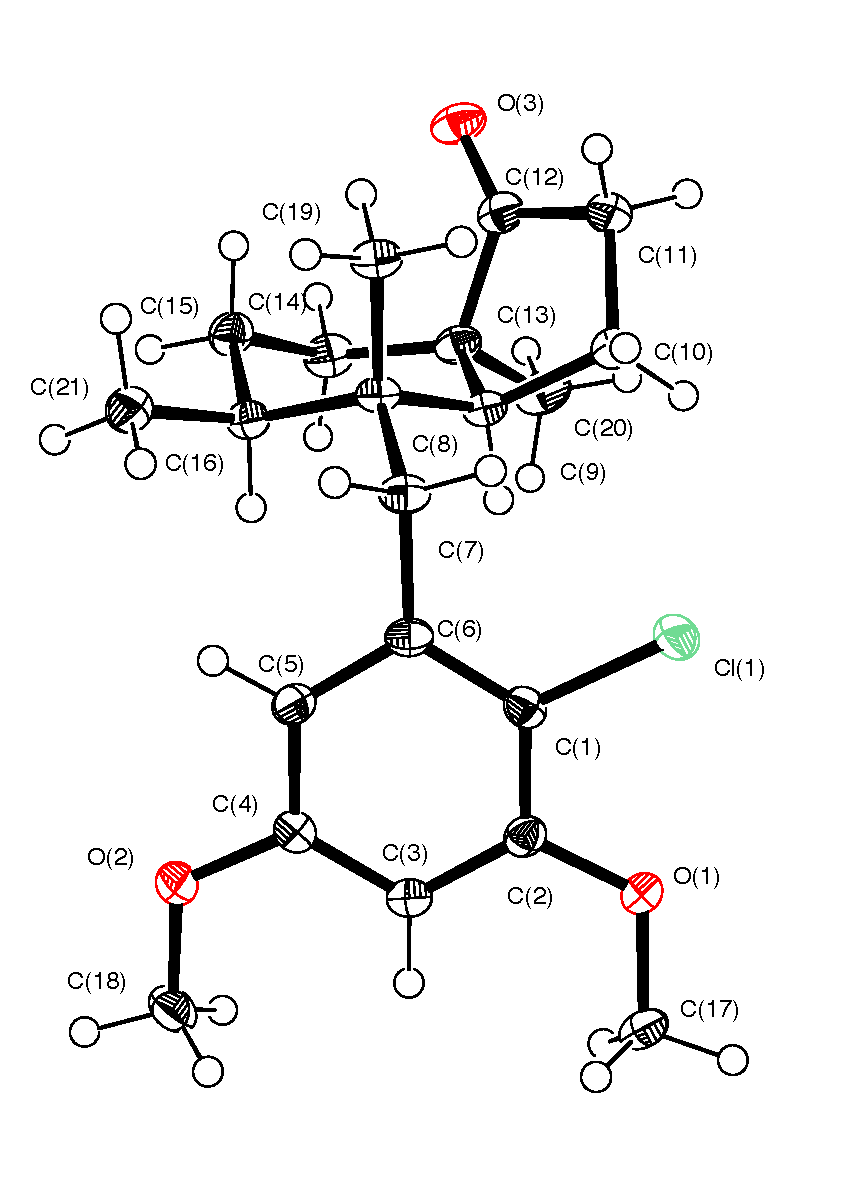
\includegraphics[width=4.2in]{chp_singlecarbon/images/xray/xbat_labelled}
    \begin{textblock}{1}(13,-13)
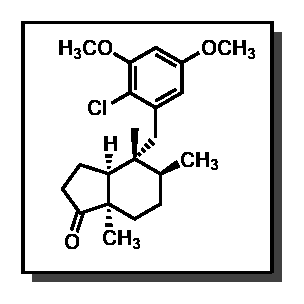
\includegraphics[scale=0.8]{chp_singlecarbon/images/xbat}
\end{textblock}
  \caption{ORTEP drawing of  $\beta$-methyl ketone \ref{cmp:xbat} shown at 50\% probability }
\end{figure}

\pagebreak

\begin{table}[h]
\centering
\caption{Crystal data and structure refinement for \ref{cmp:xbat}} 
\begin{tabular}{ll} 
\toprule
Empirical formula& 	\ce{C21H29ClO3} \\
Formula weight&	364.89 \\
Temperature &	143(2) K \\
Wavelength& 	0.71073 \AA  \\
Crystal system& 	Monoclinic \\
Space group& 	P2(1)/n \\
Unit cell dimensions&	a = 7.6944(4) \AA\ $\alpha$ = 90$^\circ$. \\
	&b = 19.9366(11)  \AA\	$\beta$ = 98.290(2)$^\circ$. \\
	&c = 12.1637(7) \AA\	$\gamma$ = 90$^\circ$. \\
Volume&	1846.42(18) \AA$^3$ \\
Z&	4 \\
Density (calculated)&	1.313 Mg/m$^3$ \\
Absorption coefficient&	0.224 mm$^{-1}$ \\
F(000) &	784 \\
Crystal size &	0.13 x 0.05 x 0.03 mm$^3$ \\
Theta range for data collection &	1.98 to 28.28$^\circ$. \\
Index ranges &	$-$10$<=$h$<=$10, $-$26$<=$k$<=$26, $-$16$<=$l$<=$16 \\
Reflections collected &	29305 \\
Independent reflections &	4583 [R(int) = 0.0305] \\
Completeness to theta = 28.28$^\circ$ &	100.0\% \\ 
Absorption correction&	Semi-empirical from equivalents \\
Max. and min. transmission &	0.9933 and 0.9714 \\
Refinement method	&Full-matrix least-squares on F$^2$ \\
Data / restraints / parameters &	 4583 / 0 / 231 \\
Goodness-of-fit on F$^2$ & 	1.021 \\
Final R indices [I$>$2sigma(I)] &	R1 = 0.0366, wR2 = 0.0840 \\
R indices (all data) &	R1 = 0.0521, wR2 = 0.0918 \\
Extinction coefficient	& na \\
Largest diff. peak and hole &	0.331 and $-$0.217 e.\AA$^{-3}$ \\
\bottomrule
\end{tabular}
\end{table}

\twocolumn
\begin{table}[h]
\centering
\caption{Atomic coordinates (x 10$^4$) and equivalent isotropic displacement parameters (\AA$^2$x
10$^3$) for \ref{cmp:xbat}}
{\footnotesize
\begin{tabular}{lcccc} 
\\
\toprule
& x & y & z & U(eq) \\
\midrule
Cl(1)&11743(1)&3756(1)&$-$1137(1)&26(1)\\
O(1)&13371(1)&4529(1)&678(1)&25(1)\\
O(2)&8389(1)&4536(1)&2701(1)&30(1)\\
O(3)&8573(1)&503(1)&$-$679(1)&28(1)\\
C(1)&10764(2)&3949(1)&30(1)&19(1)\\
C(2)&11719(2)&4356(1)&840(1)&19(1)\\
C(3)&10970(2)&4557(1)&1762(1)&20(1)\\
C(4)&9264(2)&4359(1)&1841(1)&21(1)\\
C(5)&8326(2)&3957(1)&1034(1)&21(1)\\
C(6)&9066(2)&3730(1)&123(1)&19(1)\\
C(7)&8003(2)&3284(1)&$-$733(1)&20(1)\\
C(8)&7812(2)&2525(1)&$-$443(1)&18(1)\\
C(9)&9683(2)&2206(1)&$-$231(1)&19(1)\\
C(10)&10482(2)&2082(1)&$-$1316(1)&24(1)\\
C(11)&9954(2)&1361(1)&$-$1681(1)&26(1)\\
C(12)&9314(2)&1040(1)&$-$686(1)&22(1)\\
C(13)&9783(2)&1501(1)&315(1)&21(1)\\
C(14)&8657(2)&1404(1)&1233(1)&25(1)\\
C(15)&6832(2)&1699(1)&940(1)&23(1)\\
C(16)&6900(2)&2437(1)&608(1)&20(1)\\
C(17)&14249(2)&5036(1)&1386(1)&25(1)\\
C(18)&9300(2)&4927(1)&3577(1)&29(1)\\
C(19)&6636(2)&2226(1)&$-$1463(1)&22(1)\\
C(20)&11701(2)&1318(1)&777(1)&30(1)\\
C(21)&5046(2)&2735(1)&506(1)&26(1)\\
\bottomrule
\end{tabular}
}
\end{table} 

\begin{center}
\tablefirsthead{%
\toprule}
\tablehead{%
\multicolumn{2}{c}{\footnotesize \textbf{Table \thetable} continued\ldots} \\
\toprule
}
\tabletail{%
%\midrule
\multicolumn{2}{c}{\small \ldots}\\
}
\tablelasttail{\bottomrule}
\topcaption{Bond lengths (\AA) and angles (${^\circ}$) for \ref{cmp:xbat}}
{\footnotesize \singlespacing
\begin{supertabular}{p{1.5in}c}
Cl(1)-C(1) &1.7432(13)\\
O(1)-C(2) &1.3586(16)\\
O(1)-C(17) &1.4330(16)\\
O(2)-C(4) &1.3694(16)\\
O(2)-C(18) &1.4209(17)\\
O(3)-C(12) &1.2127(16)\\
C(1)-C(6) &1.3974(19)\\
C(1)-C(2) &1.3998(18)\\
C(2)-C(3) &1.3918(18)\\
C(3)-C(4) &1.3870(19)\\
C(3)-H(3) &0.95\\
C(4)-C(5) &1.3868(18)\\
C(5)-C(6) &1.3922(18)\\
C(5)-H(5) &0.95\\
C(6)-C(7) &1.5151(18)\\
C(7)-C(8) &1.5666(18)\\
C(7)-H(7A) &0.99\\
C(7)-H(7B) &0.99\\
C(8)-C(19) &1.5452(17)\\
C(8)-C(16) &1.5541(18)\\
C(8)-C(9) &1.5607(18)\\
C(9)-C(13) &1.5533(18)\\
C(9)-C(10) &1.5534(19)\\
C(9)-H(9) &1\\
C(10)-C(11) &1.5420(19)\\
C(10)-H(10A) &0.99\\
C(10)-H(10B) &0.99\\
C(11)-C(12) &1.513(2)\\
C(11)-H(11A) &0.99\\
C(11)-H(11B) &0.99\\
C(12)-C(13) &1.5264(19)\\
C(13)-C(14) &1.5203(19)\\
C(13)-C(20) &1.5454(19)\\
C(14)-C(15) &1.516(2)\\
C(14)-H(14A) &0.99\\
C(14)-H(14B) &0.99\\
C(15)-C(16) &1.5295(19)\\
C(15)-H(15A) &0.99\\
C(15)-H(15B) &0.99\\
C(16)-C(21) &1.5340(19)\\
C(16)-H(16) &1\\
C(17)-H(17A) &0.98\\
C(17)-H(17B) &0.98\\
C(17)-H(17C) &0.98\\
C(18)-H(18A) &0.98\\
C(18)-H(18B) &0.98\\
C(18)-H(18C) &0.98\\
C(19)-H(19A) &0.98\\
C(19)-H(19B) &0.98\\
C(19)-H(19C) &0.98\\
C(20)-H(20A) &0.98\\
C(20)-H(20B) &0.98\\
C(20)-H(20C) &0.98\\
C(21)-H(21A) &0.98\\
C(21)-H(21B) &0.98\\
C(21)-H(21C) &0.98\\
C(2)-O(1)-C(17)&117.52(10)\\
C(4)-O(2)-C(18)&118.05(11)\\
C(6)-C(1)-C(2)&121.76(12)\\
C(6)-C(1)-Cl(1)&121.05(10)\\
C(2)-C(1)-Cl(1)&117.14(10)\\
O(1)-C(2)-C(3)&123.29(12)\\
O(1)-C(2)-C(1)&116.90(12)\\
C(3)-C(2)-C(1)&119.81(12)\\
C(4)-C(3)-C(2)&118.71(12)\\
C(4)-C(3)-H(3)&120.6\\
C(2)-C(3)-H(3)&120.6\\
O(2)-C(4)-C(5)&115.26(12)\\
O(2)-C(4)-C(3)&123.67(12)\\
C(5)-C(4)-C(3)&121.07(12)\\
C(4)-C(5)-C(6)&121.37(12)\\
C(4)-C(5)-H(5)&119.3\\
C(6)-C(5)-H(5)&119.3\\
C(5)-C(6)-C(1)&117.19(12)\\
C(5)-C(6)-C(7)&119.69(12)\\
C(1)-C(6)-C(7)&123.07(12)\\
C(6)-C(7)-C(8)&118.05(11)\\
C(6)-C(7)-H(7A)&107.8\\
C(8)-C(7)-H(7A)&107.8\\
C(6)-C(7)-H(7B)&107.8\\
C(8)-C(7)-H(7B)&107.8\\
H(7A)-C(7)-H(7B)&107.1\\
C(19)-C(8)-C(16)&109.57(11)\\
C(19)-C(8)-C(9)&113.28(11)\\
C(16)-C(8)-C(9)&109.46(10)\\
C(19)-C(8)-C(7)&104.78(10)\\
C(16)-C(8)-C(7)&111.27(10)\\
C(9)-C(8)-C(7)&108.43(10)\\
C(13)-C(9)-C(10)&102.57(10)\\
C(13)-C(9)-C(8)&115.25(11)\\
C(10)-C(9)-C(8)&113.14(11)\\
C(13)-C(9)-H(9)&108.5\\
C(10)-C(9)-H(9)&108.5\\
C(8)-C(9)-H(9)&108.5\\
C(11)-C(10)-C(9)&105.89(11)\\
C(11)-C(10)-H(10A)&110.6\\
C(9)-C(10)-H(10A)&110.6\\
C(11)-C(10)-H(10B)&110.6\\
C(9)-C(10)-H(10B)&110.6\\
H(10A)-C(10)-H(10B)&108.7\\
C(12)-C(11)-C(10)&105.44(11)\\
C(12)-C(11)-H(11A)&110.7\\
C(10)-C(11)-H(11A)&110.7\\
C(12)-C(11)-H(11B)&110.7\\
C(10)-C(11)-H(11B)&110.7\\
H(11A)-C(11)-H(11B)&108.8\\
O(3)-C(12)-C(11)&125.86(13)\\
O(3)-C(12)-C(13)&125.67(13)\\
C(11)-C(12)-C(13)&108.47(11)\\
C(14)-C(13)-C(12)&114.53(11)\\
C(14)-C(13)-C(20)&108.59(11)\\
C(12)-C(13)-C(20)&104.57(11)\\
C(14)-C(13)-C(9)&115.49(11)\\
C(12)-C(13)-C(9)&102.27(10)\\
C(20)-C(13)-C(9)&110.78(11)\\
C(15)-C(14)-C(13)&112.67(11)\\
C(15)-C(14)-H(14A)&109.1\\
C(13)-C(14)-H(14A)&109.1\\
C(15)-C(14)-H(14B)&109.1\\
C(13)-C(14)-H(14B)&109.1\\
H(14A)-C(14)-H(14B)&107.8\\
C(14)-C(15)-C(16)&111.64(11)\\
C(14)-C(15)-H(15A)&109.3\\
C(16)-C(15)-H(15A)&109.3\\
C(14)-C(15)-H(15B)&109.3\\
C(16)-C(15)-H(15B)&109.3\\
H(15A)-C(15)-H(15B)&108\\
C(15)-C(16)-C(21)&109.15(11)\\
C(15)-C(16)-C(8)&111.29(11)\\
C(21)-C(16)-C(8)&114.48(11)\\
C(15)-C(16)-H(16)&107.2\\
C(21)-C(16)-H(16)&107.2\\
C(8)-C(16)-H(16)&107.2\\
O(1)-C(17)-H(17A)&109.5\\
O(1)-C(17)-H(17B)&109.5\\
H(17A)-C(17)-H(17B)&109.5\\
O(1)-C(17)-H(17C)&109.5\\
H(17A)-C(17)-H(17C)&109.5\\
H(17B)-C(17)-H(17C)&109.5\\
O(2)-C(18)-H(18A)&109.5\\
O(2)-C(18)-H(18B)&109.5\\
H(18A)-C(18)-H(18B)&109.5\\
O(2)-C(18)-H(18C)&109.5\\
H(18A)-C(18)-H(18C)&109.5\\
H(18B)-C(18)-H(18C)&109.5\\
C(8)-C(19)-H(19A)&109.5\\
C(8)-C(19)-H(19B)&109.5\\
H(19A)-C(19)-H(19B)&109.5\\
C(8)-C(19)-H(19C)&109.5\\
H(19A)-C(19)-H(19C)&109.5\\
H(19B)-C(19)-H(19C)&109.5\\
C(13)-C(20)-H(20A)&109.5\\
C(13)-C(20)-H(20B)&109.5\\
H(20A)-C(20)-H(20B)&109.5\\
C(13)-C(20)-H(20C)&109.5\\
H(20A)-C(20)-H(20C)&109.5\\
H(20B)-C(20)-H(20C)&109.5\\
C(16)-C(21)-H(21A)&109.5\\
C(16)-C(21)-H(21B)&109.5\\
H(21A)-C(21)-H(21B)&109.5\\
C(16)-C(21)-H(21C)&109.5\\
H(21A)-C(21)-H(21C)&109.5\\
H(21B)-C(21)-H(21C)&109.5\\
\end{supertabular}
}
\end{center}

\begin{center}
\tablefirsthead{%
\toprule
&x&y&z&U(eq) \\
\midrule}
\tablehead{%
\multicolumn{5}{c}{\footnotesize \textbf{Table \thetable} continued\ldots} \\
\toprule
&x&y&z&U(eq) \\
\midrule
}
\tabletail{%
%\midrule
\multicolumn{5}{c}{\small \ldots}\\
}
\tablelasttail{\bottomrule}
\topcaption{Hydrogen coordinates (x 10$^4$) and isotropic displacement parameters (\AA$^2$x 10$^3$)
for \ref{cmp:xbat}} {\footnotesize \singlespacing
\begin{supertabular}{lcccc}
H(3)&11614&4824&2326&25\\
H(5)&7154&3834&1103&26\\
H(7A)&8537&3310&$-$1426&25\\
H(7B)&6808&3477&$-$898&25\\
H(9)&10478&2516&255&23\\
H(10A)&10007&2408&$-$1897&28\\
H(10B)&11776&2127&$-$1176&28\\
H(11A)&9011&1365&$-$2327&31\\
H(11B)&10975&1113&$-$1886&31\\
H(14A)&8555&919&1382&29\\
H(14B)&9246&1619&1921&29\\
H(15A)&6194&1657&1588&28\\
H(15B)&6178&1441&319&28\\
H(16)&7637&2676&1231&24\\
H(17A)&14490&4866&2149&37\\
H(17B)&13501&5435&1368&37\\
H(17C)&15358&5154&1127&37\\
H(18A)&9630&5359&3282&43\\
H(18B)&10360&4688&3909&43\\
H(18C)&8538&5004&4144&43\\
H(19A)&5496&2454&$-$1566&34\\
H(19B)&6463&1746&$-$1343&34\\
H(19C)&7205&2288&$-$2127&34\\
H(20A)&11739&866&1097&44\\
H(20B)&12162&1641&1354&44\\
H(20C)&12419&1331&174&44\\
H(21A)&4636&2722&1232&40\\
H(21B)&4248&2473&$-$31&40\\
H(21C)&5071&3201&251&40\\
\end{supertabular}
}
\end{center}

\begin{center}
\tablefirsthead{%
\toprule}
\tablehead{%
\multicolumn{2}{c}{\footnotesize \textbf{Table \thetable} continued\ldots} \\
\toprule
}
\tabletail{%
%\midrule
\multicolumn{2}{c}{\small \ldots}\\
}
\tablelasttail{\bottomrule}
\topcaption{Torsion angles ($^{\circ}$) for \ref{cmp:xbat}}
{\footnotesize \singlespacing
\begin{supertabular}{p{1.5in}c}
C(17)-O(1)-C(2)-C(3)&$-$11.31(19)\\
C(17)-O(1)-C(2)-C(1)&169.30(12)\\
C(6)-C(1)-C(2)-O(1)&178.72(12)\\
Cl(1)-C(1)-C(2)-O(1)&$-$3.98(16)\\
C(6)-C(1)-C(2)-C(3)&$-$0.7(2)\\
Cl(1)-C(1)-C(2)-C(3)&176.61(10)\\
O(1)-C(2)-C(3)-C(4)&179.20(12)\\
C(1)-C(2)-C(3)-C(4)&$-$1.42(19)\\
C(18)-O(2)-C(4)-C(5)&177.71(12)\\
C(18)-O(2)-C(4)-C(3)&$-$2.0(2)\\
C(2)-C(3)-C(4)-O(2)&$-$178.95(12)\\
C(2)-C(3)-C(4)-C(5)&1.3(2)\\
O(2)-C(4)-C(5)-C(6)&$-$178.84(12)\\
C(3)-C(4)-C(5)-C(6)&0.9(2)\\
C(4)-C(5)-C(6)-C(1)&$-$2.9(2)\\
C(4)-C(5)-C(6)-C(7)&179.28(12)\\
C(2)-C(1)-C(6)-C(5)&2.83(19)\\
Cl(1)-C(1)-C(6)-C(5)&$-$174.37(10)\\
C(2)-C(1)-C(6)-C(7)&$-$179.45(12)\\
Cl(1)-C(1)-C(6)-C(7)&3.35(18)\\
C(5)-C(6)-C(7)-C(8)&$-$77.95(16)\\
C(1)-C(6)-C(7)-C(8)&104.38(15)\\
C(6)-C(7)-C(8)-C(19)&178.68(12)\\
C(6)-C(7)-C(8)-C(16)&60.35(15)\\
C(6)-C(7)-C(8)-C(9)&$-$60.08(15)\\
C(19)-C(8)-C(9)-C(13)&$-$76.96(14)\\
C(16)-C(8)-C(9)-C(13)&45.64(14)\\
C(7)-C(8)-C(9)-C(13)&167.19(10)\\
C(19)-C(8)-C(9)-C(10)&40.63(15)\\
C(16)-C(8)-C(9)-C(10)&163.24(10)\\
C(7)-C(8)-C(9)-C(10)&$-$75.21(13)\\
C(13)-C(9)-C(10)-C(11)&33.10(13)\\
C(8)-C(9)-C(10)-C(11)&$-$91.69(13)\\
C(9)-C(10)-C(11)-C(12)&$-$14.10(14)\\
C(10)-C(11)-C(12)-O(3)&169.94(13)\\
C(10)-C(11)-C(12)-C(13)&$-$10.96(14)\\
O(3)-C(12)-C(13)-C(14)&$-$23.79(19)\\
C(11)-C(12)-C(13)-C(14)&157.11(11)\\
O(3)-C(12)-C(13)-C(20)&94.94(16)\\
C(11)-C(12)-C(13)-C(20)&$-$84.15(13)\\
O(3)-C(12)-C(13)-C(9)&$-$149.49(13)\\
C(11)-C(12)-C(13)-C(9)&31.42(13)\\
C(10)-C(9)-C(13)-C(14)&$-$163.91(11)\\
C(8)-C(9)-C(13)-C(14)&$-$40.52(16)\\
C(10)-C(9)-C(13)-C(12)&$-$38.85(12)\\
C(8)-C(9)-C(13)-C(12)&84.55(13)\\
C(10)-C(9)-C(13)-C(20)&72.12(13)\\
C(8)-C(9)-C(13)-C(20)&$-$164.48(12)\\
C(12)-C(13)-C(14)-C(15)&$-$74.90(15)\\
C(20)-C(13)-C(14)-C(15)&168.66(11)\\
C(9)-C(13)-C(14)-C(15)&43.55(16)\\
C(13)-C(14)-C(15)-C(16)&$-$54.11(16)\\
C(14)-C(15)-C(16)-C(21)&$-$170.94(11)\\
C(14)-C(15)-C(16)-C(8)&61.74(15)\\
C(19)-C(8)-C(16)-C(15)&68.73(14)\\
C(9)-C(8)-C(16)-C(15)&$-$56.06(13)\\
C(7)-C(8)-C(16)-C(15)&$-$175.88(11)\\
C(19)-C(8)-C(16)-C(21)&$-$55.63(14)\\
C(9)-C(8)-C(16)-C(21)&179.59(11)\\
C(7)-C(8)-C(16)-C(21)&59.76(14)\\
\end{supertabular}
}
\end{center}

\onecolumn
\begin{table}[h]
\centering
\caption{Anisotropic displacement parameters (\AA$^2$x 10$^3$) for \ref{cmp:xbat}} 
\footnotesize
\begin{tabular}{p{1in}cccccc} 
\toprule
& U$^{11}$ & U$^{22}$ & U$^{33}$ & U$^{23}$ & U$^{13}$ & U$^{12}$ \\
\midrule
Cl(1)&33(1) &25(1)&22(1) &$-$4(1)&10(1) &$-$5(1)\\
O(1)&22(1) &27(1)&29(1) &$-$7(1)&8(1) &$-$8(1)\\
O(2)&26(1) &38(1)&28(1) &$-$15(1)&10(1) &$-$8(1)\\
O(3)&27(1) &17(1)&38(1) &$-$1(1)&$-$2(1) &$-$3(1)\\
C(1)&25(1) &17(1)&17(1) &1(1)&5(1) &0(1)\\
C(2)&19(1) &16(1)&23(1) &2(1)&4(1) &$-$1(1)\\
C(3)&22(1) &18(1)&21(1) &$-$2(1)&1(1) &$-$2(1)\\
C(4)&22(1) &20(1)&21(1) &$-$2(1)&4(1) &0(1)\\
C(5)&19(1) &19(1)&26(1) &$-$2(1)&3(1) &$-$2(1)\\
C(6)&23(1) &14(1)&19(1) &1(1)&0(1) &0(1)\\
C(7)&25(1) &16(1)&19(1) &0(1)&$-$2(1) &$-$1(1)\\
C(8)&20(1) &16(1)&17(1) &0(1)&$-$1(1) &$-$2(1)\\
C(9)&19(1) &16(1)&21(1) &$-$1(1)&0(1) &$-$3(1)\\
C(10)&25(1) &22(1)&26(1) &$-$3(1)&6(1) &$-$4(1)\\
C(11)&26(1) &22(1)&29(1) &$-$7(1)&6(1) &$-$2(1)\\
C(12)&17(1) &18(1)&31(1) &$-$1(1)&$-$1(1) &3(1)\\
C(13)&21(1) &16(1)&25(1) &1(1)&$-$1(1) &$-$1(1)\\
C(14)&29(1) &21(1)&23(1) &5(1)&0(1) &$-$2(1)\\
C(15)&26(1) &23(1)&22(1) &2(1)&5(1) &$-$4(1)\\
C(16)&20(1) &19(1)&20(1) &$-$2(1)&1(1) &$-$2(1)\\
C(17)&23(1) &21(1)&30(1) &$-$1(1)&3(1) &$-$7(1)\\
C(18)&27(1) &34(1)&25(1) &$-$12(1)&3(1) &3(1)\\
C(19)&24(1) &20(1)&22(1) &$-$1(1)&$-$3(1) &$-$2(1)\\
C(20)&23(1) &24(1)&39(1) &2(1)&$-$6(1) &1(1)\\
C(21)&22(1) &26(1)&31(1) &$-$3(1)&3(1) &$-$1(1)\\
\bottomrule
\end{tabular}
\end{table}
{ \footnotesize
The anisotropic displacement factor exponent takes the form: 
$-2\pi^2\left[ h^2a*^2U^{11} + ... + 2 h k a* b* U^{12} \right]$ }

\pagebreak
%%%%%%%%%%% End of X-Ray Data for xbat %%%%%%%%%%%%%%%%%%%%

%%%%%%%%%%% Begin  X-Ray Data for xbau %%%%%%%%%%%%%%%%%%%%
\subsection{Structural Data for $\alpha$-methyl Ketone \ref{cmp:xbau}}
Suitable crystals for X-ray analysis were obtained by
crystallization from hot Et$_2$O and hexanes (approx. 5:1 v/v).
\begin{figure}[h]
 % \centering
  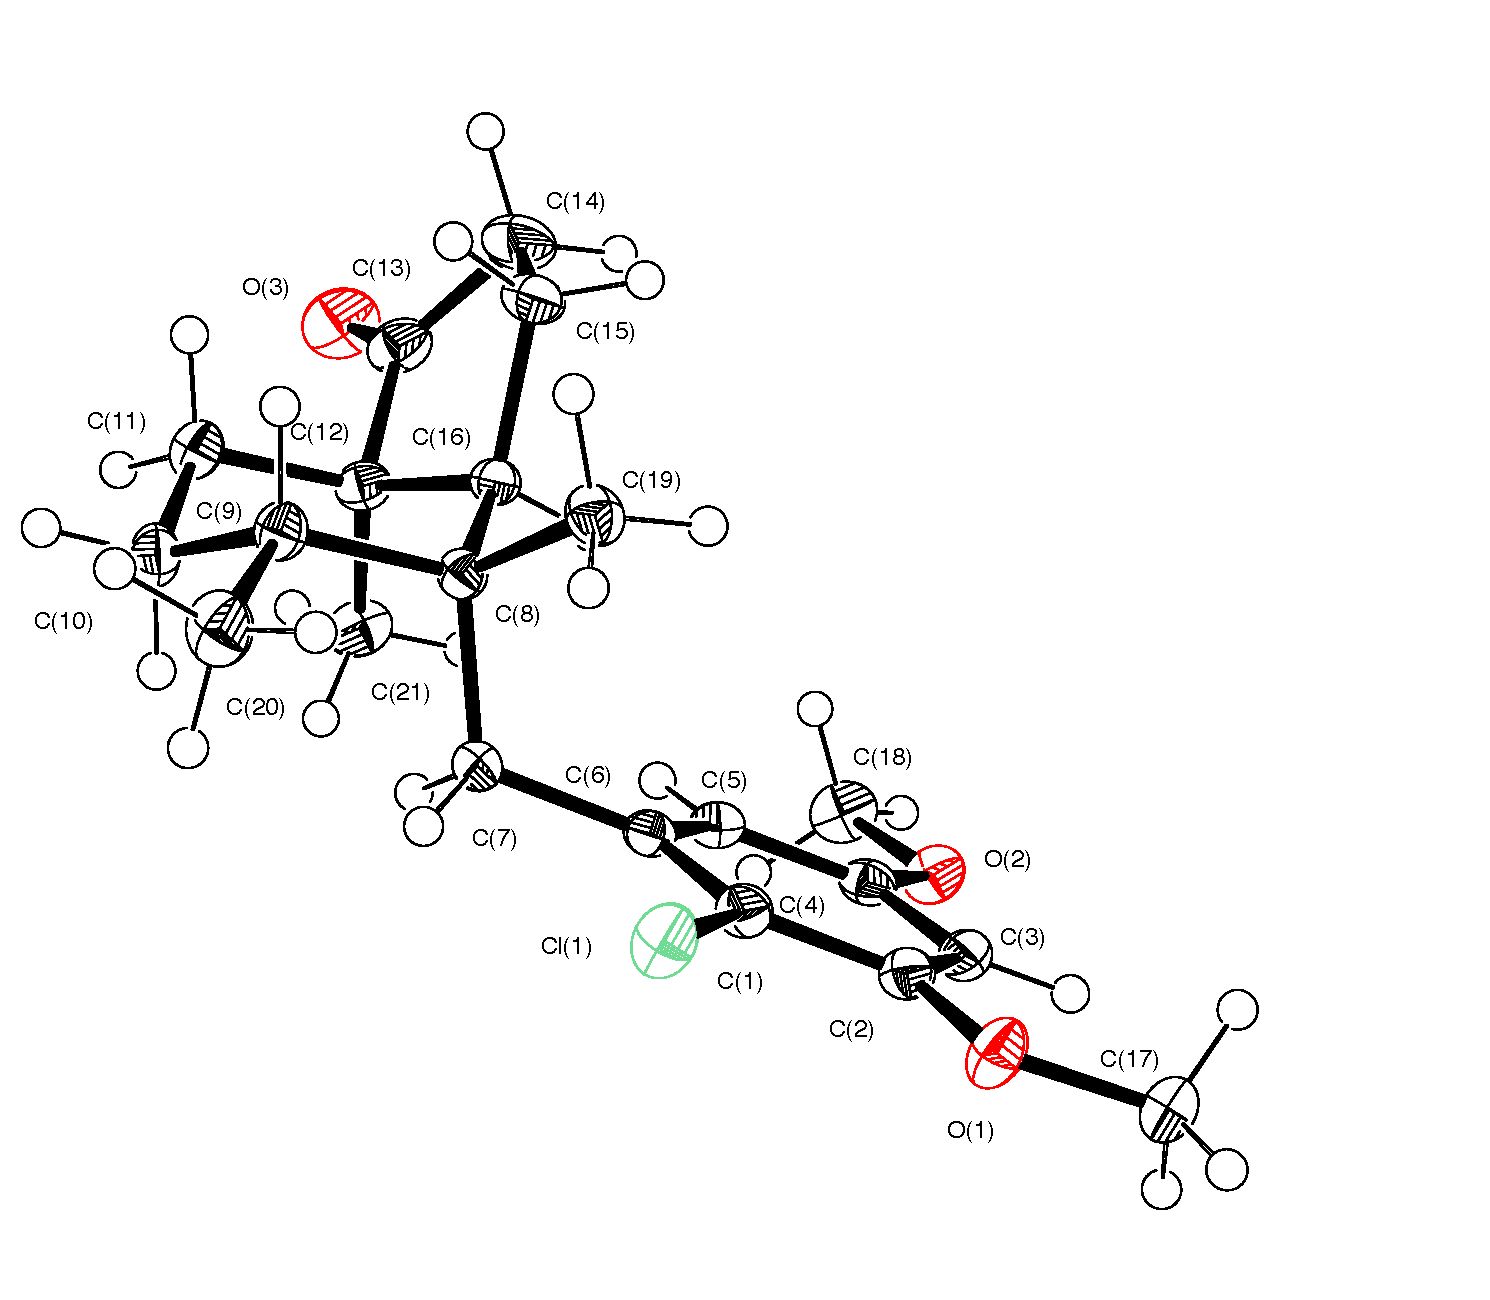
\includegraphics[width=6in]{chp_singlecarbon/images/xray/xbau_labelled}
    \begin{textblock}{1}(12,-14)
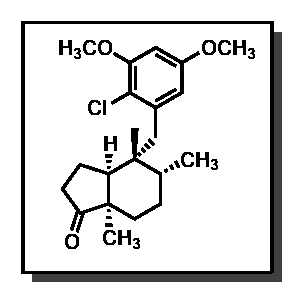
\includegraphics[scale=0.8]{chp_singlecarbon/images/xbau}
\end{textblock}
  \caption{ORTEP drawing of  $\alpha$-methyl ketone \ref{cmp:xbau} shown at 50\% probability }
\end{figure}

\pagebreak

\begin{table}[h]
\centering
\caption{Crystal data and structure refinement for \ref{cmp:xbau}} 
\begin{tabular}{ll} 
\toprule
Empirical formula& 	\ce{C21H29ClO3} \\
Formula weight&	364.89 \\
Temperature &	143(2) K \\
Wavelength& 	0.71073 \AA  \\
Crystal system& 	Monoclinic \\
Space group& 	P2(1)/c \\
Unit cell dimensions&	a = 17.3130(12)  \AA\ $\alpha$ = 90$^\circ$. \\
	&b = 7.2226(5)  \AA\	$\beta$ = 101.394(3)$^\circ$. \\
	&c = 15.0735(11)  \AA\	$\gamma$ = 90$^\circ$. \\
Volume&	1847.7(2) \AA$^3$ \\
Z&	4 \\
Density (calculated)&	1.312 Mg/m$^3$ \\
Absorption coefficient&	0.224 mm$^{-1}$ \\
F(000) &	784 \\
Crystal size &	0.15 x 0.12 x 0.08 mm$^3$ \\
Theta range for data collection &	2.40 to 28.00$^\circ$. \\
Index ranges &	$-$22$<=$h$<=$22, $-$8$<=$k$<=$9, $-$17$<=$l$<=$19 \\
Reflections collected &	26894 \\
Independent reflections &	4435 [R(int) = 0.0200] \\
Completeness to theta = 28.00$^\circ$ &	99.5\% \\ 
Absorption correction&	Semi-empirical from equivalents \\
Max. and min. transmission &	0.9823 and 0.9672 \\
Refinement method	&Full-matrix least-squares on F$^2$ \\
Data / restraints / parameters &	 4435 / 0 / 231 \\
Goodness-of-fit on F$^2$ & 	1.039 \\
Final R indices [I$>$2sigma(I)] &	R1 = 0.0330, wR2 = 0.0908 \\
R indices (all data) &	R1 = 0.0355, wR2 = 0.0930 \\
Extinction coefficient	& na \\
Largest diff. peak and hole &	0.344 and $-$0.266 e.\AA$^{-3}$ \\
\bottomrule
\end{tabular}
\end{table}

\twocolumn
\begin{table}[h]
\centering
\caption{Atomic coordinates (x 10$^4$) and equivalent isotropic displacement parameters (\AA$^2$x
10$^3$) for \ref{cmp:xbau}}
{\footnotesize
\begin{tabular}{lcccc} 
\\
\toprule
& x & y & z & U(eq) \\
\midrule
Cl(1)&4508(1)&6621(1)&10743(1)&27(1)\\
O(1)&4403(1)&3107(1)&11520(1)&26(1)\\
O(2)&1637(1)&2254(1)&10639(1)&25(1)\\
O(3)&85(1)&8494(1)&6962(1)&39(1)\\
C(1)&3631(1)&5405(1)&10664(1)&20(1)\\
C(2)&3675(1)&3667(1)&11094(1)&20(1)\\
C(3)&2994(1)&2645(1)&11066(1)&21(1)\\
C(4)&2274(1)&3369(1)&10624(1)&20(1)\\
C(5)&2231(1)&5085(1)&10207(1)&19(1)\\
C(6)&2917(1)&6124(1)&10207(1)&18(1)\\
C(7)&2858(1)&7988(1)&9742(1)&18(1)\\
C(8)&2839(1)&7974(1)&8700(1)&17(1)\\
C(9)&3007(1)&9966(1)&8390(1)&21(1)\\
C(10)&2317(1)&11278(1)&8402(1)&24(1)\\
C(11)&1567(1)&10611(2)&7781(1)&24(1)\\
C(12)&1325(1)&8661(2)&8049(1)&20(1)\\
C(13)&756(1)&7952(2)&7208(1)&27(1)\\
C(14)&1163(1)&6530(2)&6732(1)&33(1)\\
C(15)&2034(1)&6688(2)&7172(1)&25(1)\\
C(16)&2029(1)&7290(1)&8157(1)&18(1)\\
C(17)&4470(1)&1305(2)&11916(1)&28(1)\\
C(18)&882(1)&2956(2)&10224(1)&30(1)\\
C(19)&3484(1)&6661(2)&8502(1)&23(1)\\
C(20)&3771(1)&10832(2)&8913(1)&29(1)\\
C(21)&891(1)&8761(2)&8837(1)&27(1)\\
\bottomrule
\end{tabular}
}
\end{table} 

\begin{center}
\tablefirsthead{%
\toprule}
\tablehead{%
\multicolumn{2}{c}{\footnotesize \textbf{Table \thetable} continued\ldots} \\
\toprule
}
\tabletail{%
%\midrule
\multicolumn{2}{c}{\small \ldots}\\
}
\tablelasttail{\bottomrule}
\topcaption{Bond lengths (\AA) and angles (${^\circ}$) for \ref{cmp:xbau}}
{\footnotesize \singlespacing
\begin{supertabular}{p{1.5in}c}
Cl(1)-C(1) &1.7381(10)\\
O(1)-C(2) &1.3585(13)\\
O(1)-C(17) &1.4269(13)\\
O(2)-C(4) &1.3696(12)\\
O(2)-C(18) &1.4256(14)\\
O(3)-C(13) &1.2120(15)\\
C(1)-C(6) &1.3905(14)\\
C(1)-C(2) &1.4078(14)\\
C(2)-C(3) &1.3836(14)\\
C(3)-C(4) &1.3943(15)\\
C(3)-H(3) &0.95\\
C(4)-C(5) &1.3848(14)\\
C(5)-C(6) &1.4051(14)\\
C(5)-H(5) &0.95\\
C(6)-C(7) &1.5119(14)\\
C(7)-C(8) &1.5652(13)\\
C(7)-H(7A) &0.99\\
C(7)-H(7B) &0.99\\
C(8)-C(19) &1.5377(13)\\
C(8)-C(9) &1.5571(13)\\
C(8)-C(16) &1.5579(13)\\
C(9)-C(10) &1.5271(15)\\
C(9)-C(20) &1.5343(15)\\
C(9)-H(9) &1\\
C(10)-C(11) &1.5199(15)\\
C(10)-H(10A) &0.99\\
C(10)-H(10B) &0.99\\
C(11)-C(12) &1.5453(15)\\
C(11)-H(11A) &0.99\\
C(11)-H(11B) &0.99\\
C(12)-C(21) &1.5271(14)\\
C(12)-C(13) &1.5323(15)\\
C(12)-C(16) &1.5539(14)\\
C(13)-C(14) &1.5053(18)\\
C(14)-C(15) &1.5266(17)\\
C(14)-H(14A) &0.99\\
C(14)-H(14B) &0.99\\
C(15)-C(16) &1.5481(14)\\
C(15)-H(15A) &0.99\\
C(15)-H(15B) &0.99\\
C(16)-H(16) &1\\
C(17)-H(17A) &0.98\\
C(17)-H(17B) &0.98\\
C(17)-H(17C) &0.98\\
C(18)-H(18A) &0.98\\
C(18)-H(18B) &0.98\\
C(18)-H(18C) &0.98\\
C(19)-H(19A) &0.98\\
C(19)-H(19B) &0.98\\
C(19)-H(19C) &0.98\\
C(20)-H(20A) &0.98\\
C(20)-H(20B) &0.98\\
C(20)-H(20C) &0.98\\
C(21)-H(21A) &0.98\\
C(21)-H(21B) &0.98\\
C(21)-H(21C) &0.98\\
C(2)-O(1)-C(17)&117.45(9)\\
C(4)-O(2)-C(18)&117.05(9)\\
C(6)-C(1)-C(2)&121.55(9)\\
C(6)-C(1)-Cl(1)&121.59(8)\\
C(2)-C(1)-Cl(1)&116.85(8)\\
O(1)-C(2)-C(3)&124.07(9)\\
O(1)-C(2)-C(1)&116.38(9)\\
C(3)-C(2)-C(1)&119.54(10)\\
C(2)-C(3)-C(4)&119.35(9)\\
C(2)-C(3)-H(3)&120.3\\
C(4)-C(3)-H(3)&120.3\\
O(2)-C(4)-C(5)&124.23(9)\\
O(2)-C(4)-C(3)&114.75(9)\\
C(5)-C(4)-C(3)&121.02(9)\\
C(4)-C(5)-C(6)&120.55(9)\\
C(4)-C(5)-H(5)&119.7\\
C(6)-C(5)-H(5)&119.7\\
C(1)-C(6)-C(5)&117.94(9)\\
C(1)-C(6)-C(7)&122.33(9)\\
C(5)-C(6)-C(7)&119.70(9)\\
C(6)-C(7)-C(8)&116.50(8)\\
C(6)-C(7)-H(7A)&108.2\\
C(8)-C(7)-H(7A)&108.2\\
C(6)-C(7)-H(7B)&108.2\\
C(8)-C(7)-H(7B)&108.2\\
H(7A)-C(7)-H(7B)&107.3\\
C(19)-C(8)-C(9)&109.06(8)\\
C(19)-C(8)-C(16)&108.36(8)\\
C(9)-C(8)-C(16)&109.72(8)\\
C(19)-C(8)-C(7)&109.06(8)\\
C(9)-C(8)-C(7)&109.08(8)\\
C(16)-C(8)-C(7)&111.53(7)\\
C(10)-C(9)-C(20)&109.78(9)\\
C(10)-C(9)-C(8)&112.16(8)\\
C(20)-C(9)-C(8)&114.56(9)\\
C(10)-C(9)-H(9)&106.6\\
C(20)-C(9)-H(9)&106.6\\
C(8)-C(9)-H(9)&106.6\\
C(11)-C(10)-C(9)&111.77(9)\\
C(11)-C(10)-H(10A)&109.3\\
C(9)-C(10)-H(10A)&109.3\\
C(11)-C(10)-H(10B)&109.3\\
C(9)-C(10)-H(10B)&109.3\\
H(10A)-C(10)-H(10B)&107.9\\
C(10)-C(11)-C(12)&111.79(9)\\
C(10)-C(11)-H(11A)&109.3\\
C(12)-C(11)-H(11A)&109.3\\
C(10)-C(11)-H(11B)&109.3\\
C(12)-C(11)-H(11B)&109.3\\
H(11A)-C(11)-H(11B)&107.9\\
C(21)-C(12)-C(13)&108.92(9)\\
C(21)-C(12)-C(11)&111.15(9)\\
C(13)-C(12)-C(11)&104.61(9)\\
C(21)-C(12)-C(16)&116.41(9)\\
C(13)-C(12)-C(16)&103.68(9)\\
C(11)-C(12)-C(16)&111.11(8)\\
O(3)-C(13)-C(14)&125.81(11)\\
O(3)-C(13)-C(12)&124.49(11)\\
C(14)-C(13)-C(12)&109.68(9)\\
C(13)-C(14)-C(15)&104.93(9)\\
C(13)-C(14)-H(14A)&110.8\\
C(15)-C(14)-H(14A)&110.8\\
C(13)-C(14)-H(14B)&110.8\\
C(15)-C(14)-H(14B)&110.8\\
H(14A)-C(14)-H(14B)&108.8\\
C(14)-C(15)-C(16)&104.21(9)\\
C(14)-C(15)-H(15A)&110.9\\
C(16)-C(15)-H(15A)&110.9\\
C(14)-C(15)-H(15B)&110.9\\
C(16)-C(15)-H(15B)&110.9\\
H(15A)-C(15)-H(15B)&108.9\\
C(15)-C(16)-C(12)&103.39(8)\\
C(15)-C(16)-C(8)&114.70(8)\\
C(12)-C(16)-C(8)&117.31(8)\\
C(15)-C(16)-H(16)&106.9\\
C(12)-C(16)-H(16)&106.9\\
C(8)-C(16)-H(16)&106.9\\
O(1)-C(17)-H(17A)&109.5\\
O(1)-C(17)-H(17B)&109.5\\
H(17A)-C(17)-H(17B)&109.5\\
O(1)-C(17)-H(17C)&109.5\\
H(17A)-C(17)-H(17C)&109.5\\
H(17B)-C(17)-H(17C)&109.5\\
O(2)-C(18)-H(18A)&109.5\\
O(2)-C(18)-H(18B)&109.5\\
H(18A)-C(18)-H(18B)&109.5\\
O(2)-C(18)-H(18C)&109.5\\
H(18A)-C(18)-H(18C)&109.5\\
H(18B)-C(18)-H(18C)&109.5\\
C(8)-C(19)-H(19A)&109.5\\
C(8)-C(19)-H(19B)&109.5\\
H(19A)-C(19)-H(19B)&109.5\\
C(8)-C(19)-H(19C)&109.5\\
H(19A)-C(19)-H(19C)&109.5\\
H(19B)-C(19)-H(19C)&109.5\\
C(9)-C(20)-H(20A)&109.5\\
C(9)-C(20)-H(20B)&109.5\\
H(20A)-C(20)-H(20B)&109.5\\
C(9)-C(20)-H(20C)&109.5\\
H(20A)-C(20)-H(20C)&109.5\\
H(20B)-C(20)-H(20C)&109.5\\
C(12)-C(21)-H(21A)&109.5\\
C(12)-C(21)-H(21B)&109.5\\
H(21A)-C(21)-H(21B)&109.5\\
C(12)-C(21)-H(21C)&109.5\\
H(21A)-C(21)-H(21C)&109.5\\
H(21B)-C(21)-H(21C)&109.5\\
\end{supertabular}
}
\end{center}

\begin{center}
\tablefirsthead{%
\toprule
&x&y&z&U(eq) \\
\midrule}
\tablehead{%
\multicolumn{5}{c}{\footnotesize \textbf{Table \thetable} continued\ldots} \\
\toprule
&x&y&z&U(eq) \\
\midrule
}
\tabletail{%
%\midrule
\multicolumn{5}{c}{\small \ldots}\\
}
\tablelasttail{\bottomrule}
\topcaption{Hydrogen coordinates (x 10$^4$) and isotropic displacement parameters (\AA$^2$x 10$^3$)
for \ref{cmp:xbau}} {\footnotesize \singlespacing
\begin{supertabular}{lcccc}
H(3)&3018&1462&11345&25\\
H(5)&1734&5564&9919&23\\
H(7A)&3311&8751&10037&22\\
H(7B)&2374&8609&9846&22\\
H(9)&3066&9867&7745&25\\
H(10A)&2224&11377&9027&28\\
H(10B)&2452&12525&8207&28\\
H(11A)&1650&10581&7150&29\\
H(11B)&1136&11494&7809&29\\
H(14A)&1081&6797&6076&40\\
H(14B)&962&5272&6817&40\\
H(15A)&2300&7624&6859&30\\
H(15B)&2305&5483&7160&30\\
H(16)&1880&6176&8480&21\\
H(17A)&4138&1229&12372&41\\
H(17B)&5020&1072&12204&41\\
H(17C)&4298&376&11445&41\\
H(18A)&775&4095&10532&44\\
H(18B)&478&2032&10270&44\\
H(18C)&876&3224&9586&44\\
H(19A)&3338&5379&8605&35\\
H(19B)&3985&6958&8904&35\\
H(19C)&3538&6809&7871&35\\
H(20A)&3921&11879&8569&43\\
H(20B)&4192&9903&9002&43\\
H(20C)&3690&11269&9504&43\\
H(21A)&401&9460&8651&41\\
H(21B)&1225&9381&9352&41\\
H(21C)&769&7505&9013&41\\
\end{supertabular}
}
\end{center}

\begin{center}
\tablefirsthead{%
\toprule}
\tablehead{%
\multicolumn{2}{c}{\footnotesize \textbf{Table \thetable} continued\ldots} \\
\toprule
}
\tabletail{%
%\midrule
\multicolumn{2}{c}{\small \ldots}\\
}
\tablelasttail{\bottomrule}
\topcaption{Torsion angles ($^{\circ}$) for \ref{cmp:xbau}}
{\footnotesize \singlespacing
\begin{supertabular}{p{1.5in}c}
C(17)-O(1)-C(2)-C(3)&3.82(15)\\
C(17)-O(1)-C(2)-C(1)&$-$176.46(9)\\
C(6)-C(1)-C(2)-O(1)&$-$179.90(9)\\
Cl(1)-C(1)-C(2)-O(1)&$-$0.66(12)\\
C(6)-C(1)-C(2)-C(3)&$-$0.17(15)\\
Cl(1)-C(1)-C(2)-C(3)&179.07(8)\\
O(1)-C(2)-C(3)-C(4)&178.71(9)\\
C(1)-C(2)-C(3)-C(4)&$-$1.01(15)\\
C(18)-O(2)-C(4)-C(5)&$-$2.26(14)\\
C(18)-O(2)-C(4)-C(3)&177.88(9)\\
C(2)-C(3)-C(4)-O(2)&$-$179.63(9)\\
C(2)-C(3)-C(4)-C(5)&0.51(15)\\
O(2)-C(4)-C(5)-C(6)&$-$178.68(9)\\
C(3)-C(4)-C(5)-C(6)&1.16(15)\\
C(2)-C(1)-C(6)-C(5)&1.79(15)\\
Cl(1)-C(1)-C(6)-C(5)&$-$177.41(7)\\
C(2)-C(1)-C(6)-C(7)&179.99(9)\\
Cl(1)-C(1)-C(6)-C(7)&0.79(14)\\
C(4)-C(5)-C(6)-C(1)&$-$2.28(14)\\
C(4)-C(5)-C(6)-C(7)&179.48(9)\\
C(1)-C(6)-C(7)-C(8)&97.30(11)\\
C(5)-C(6)-C(7)-C(8)&$-$84.53(11)\\
C(6)-C(7)-C(8)-C(19)&$-$45.73(11)\\
C(6)-C(7)-C(8)-C(9)&$-$164.75(8)\\
C(6)-C(7)-C(8)-C(16)&73.90(10)\\
C(19)-C(8)-C(9)-C(10)&169.47(9)\\
C(16)-C(8)-C(9)-C(10)&50.93(11)\\
C(7)-C(8)-C(9)-C(10)&$-$71.52(10)\\
C(19)-C(8)-C(9)-C(20)&$-$64.51(11)\\
C(16)-C(8)-C(9)-C(20)&176.95(8)\\
C(7)-C(8)-C(9)-C(20)&54.50(11)\\
C(20)-C(9)-C(10)-C(11)&171.84(9)\\
C(8)-C(9)-C(10)-C(11)&$-$59.58(11)\\
C(9)-C(10)-C(11)-C(12)&58.82(11)\\
C(10)-C(11)-C(12)-C(21)&80.97(11)\\
C(10)-C(11)-C(12)-C(13)&$-$161.63(9)\\
C(10)-C(11)-C(12)-C(16)&$-$50.37(11)\\
C(21)-C(12)-C(13)-O(3)&45.20(15)\\
C(11)-C(12)-C(13)-O(3)&$-$73.71(13)\\
C(16)-C(12)-C(13)-O(3)&169.77(11)\\
C(21)-C(12)-C(13)-C(14)&$-$136.13(10)\\
C(11)-C(12)-C(13)-C(14)&104.96(10)\\
C(16)-C(12)-C(13)-C(14)&$-$11.56(11)\\
O(3)-C(13)-C(14)-C(15)&166.64(12)\\
C(12)-C(13)-C(14)-C(15)&$-$12.01(13)\\
C(13)-C(14)-C(15)-C(16)&30.94(12)\\
C(14)-C(15)-C(16)-C(12)&$-$38.15(11)\\
C(14)-C(15)-C(16)-C(8)&$-$167.09(9)\\
C(21)-C(12)-C(16)-C(15)&149.71(9)\\
C(13)-C(12)-C(16)-C(15)&30.14(10)\\
C(11)-C(12)-C(16)-C(15)&$-$81.72(10)\\
C(21)-C(12)-C(16)-C(8)&$-$82.98(11)\\
C(13)-C(12)-C(16)-C(8)&157.46(8)\\
C(11)-C(12)-C(16)-C(8)&45.60(11)\\
C(19)-C(8)-C(16)-C(15)&$-$42.86(11)\\
C(9)-C(8)-C(16)-C(15)&76.12(10)\\
C(7)-C(8)-C(16)-C(15)&$-$162.90(8)\\
C(19)-C(8)-C(16)-C(12)&$-$164.47(8)\\
C(9)-C(8)-C(16)-C(12)&$-$45.49(11)\\
C(7)-C(8)-C(16)-C(12)&75.48(10)\\
\end{supertabular}
}
\end{center}

\onecolumn
\begin{table}[h]
\centering
\caption{Anisotropic displacement parameters (\AA$^2$x 10$^3$) for \ref{cmp:xbau}} 
\footnotesize
\begin{tabular}{p{1in}cccccc} 
\toprule
& U$^{11}$ & U$^{22}$ & U$^{33}$ & U$^{23}$ & U$^{13}$ & U$^{12}$ \\
\midrule
Cl(1)&20(1) &26(1)&33(1) &5(1)&$-$3(1) &$-$7(1)\\
O(1)&22(1) &25(1)&30(1) &8(1)&$-$1(1) &1(1)\\
O(2)&21(1) &28(1)&26(1) &4(1)&5(1) &$-$6(1)\\
O(3)&25(1) &51(1)&37(1) &2(1)&$-$7(1) &$-$2(1)\\
C(1)&19(1) &20(1)&19(1) &$-$1(1)&2(1) &$-$4(1)\\
C(2)&21(1) &21(1)&18(1) &0(1)&2(1) &1(1)\\
C(3)&25(1) &20(1)&18(1) &2(1)&6(1) &$-$1(1)\\
C(4)&21(1) &23(1)&16(1) &$-$2(1)&6(1) &$-$5(1)\\
C(5)&18(1) &23(1)&16(1) &$-$1(1)&4(1) &0(1)\\
C(6)&21(1) &18(1)&15(1) &$-$2(1)&4(1) &$-$1(1)\\
C(7)&20(1) &17(1)&18(1) &$-$1(1)&2(1) &0(1)\\
C(8)&17(1) &16(1)&18(1) &$-$1(1)&5(1) &$-$1(1)\\
C(9)&21(1) &18(1)&23(1) &1(1)&6(1) &$-$4(1)\\
C(10)&27(1) &16(1)&28(1) &1(1)&5(1) &$-$1(1)\\
C(11)&25(1) &22(1)&25(1) &4(1)&3(1) &2(1)\\
C(12)&18(1) &24(1)&18(1) &1(1)&2(1) &$-$1(1)\\
C(13)&25(1) &33(1)&22(1) &3(1)&0(1) &$-$7(1)\\
C(14)&34(1) &40(1)&23(1) &$-$8(1)&0(1) &$-$7(1)\\
C(15)&29(1) &28(1)&19(1) &$-$5(1)&6(1) &$-$3(1)\\
C(16)&20(1) &18(1)&16(1) &$-$1(1)&4(1) &$-$2(1)\\
C(17)&32(1) &24(1)&26(1) &5(1)&2(1) &5(1)\\
C(18)&20(1) &37(1)&31(1) &2(1)&4(1) &$-$6(1)\\
C(19)&22(1) &23(1)&25(1) &$-$2(1)&8(1) &2(1)\\
C(20)&24(1) &26(1)&35(1) &1(1)&6(1) &$-$9(1)\\
C(21)&21(1) &37(1)&25(1) &4(1)&8(1) &5(1)\\
\bottomrule
\end{tabular}
\end{table}
{ \footnotesize
The anisotropic displacement factor exponent takes the form: 
$-2\pi^2\left[ h^2a*^2U^{11} + ... + 2 h k a* b* U^{12} \right]$ }
%%%%%%%%%%% End of X-Ray Data for xbau %%%%%%%%%%%%%%%%%%%%
\pagebreak

%%%%%%%%%%% Begin  X-Ray Data for xcad %%%%%%%%%%%%%%%%%%%%
\subsection{Structural Data for Imidazolium Salt \ref{cmp:xcad}}
Suitable crystals for X-ray analysis were obtained by slow diffusion of Et$_2$O into a \ce{CH2Cl2}
solution.
\begin{figure}[h]
 % \centering
  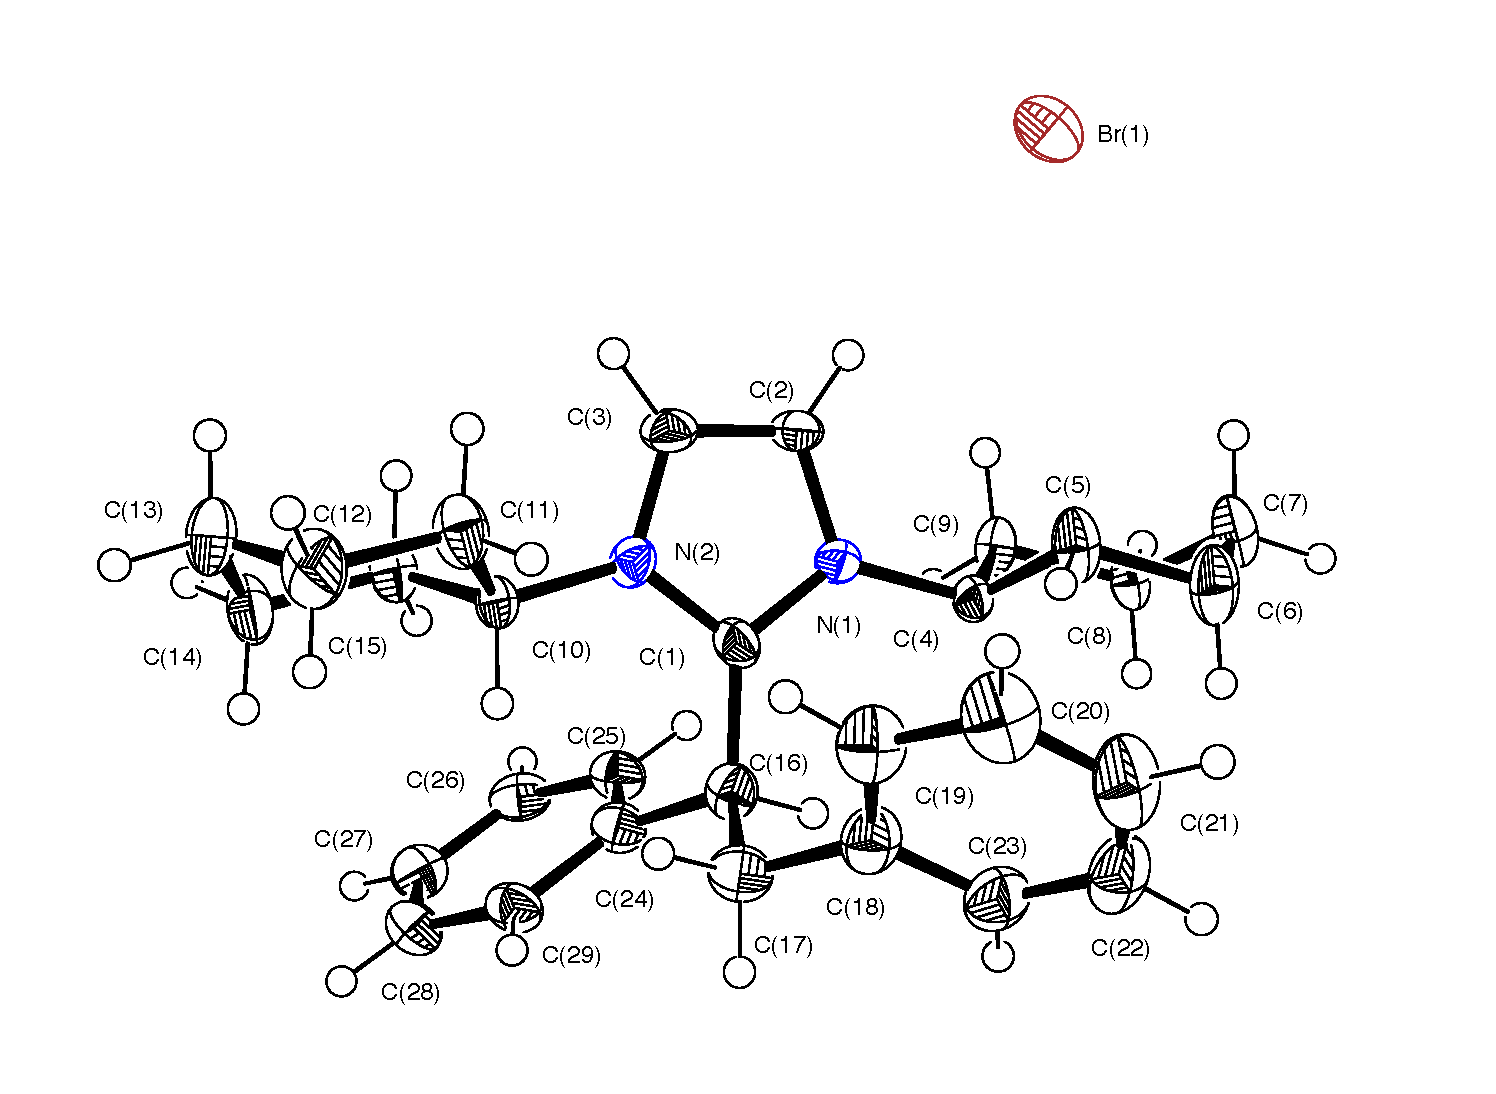
\includegraphics[width=6in]{chp_alkylation/images/xray/xcad_labelled}
    \begin{textblock}{1}(2,-13)
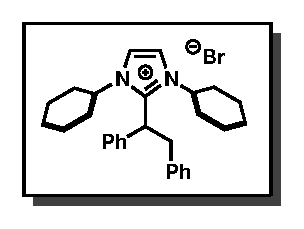
\includegraphics[scale=0.8]{chp_alkylation/images/xcad}
\end{textblock}
  \caption{ORTEP drawing of  imidazolium salt \ref{cmp:xcad} shown at 50\% probability }
\end{figure}

\pagebreak
\begin{table}[h]
\centering
\caption{Crystal data and structure refinement for \ref{cmp:xcad}} 
\begin{tabular}{ll} 
\toprule
Empirical formula& 	\ce{C29H37BrN2} \\
Formula weight&	493.52 \\
Temperature &	100(2) K \\
Wavelength& 	0.71073 \AA  \\
Crystal system& 	Orthorhombic \\
Space group& 	Fdd2 \\
Unit cell dimensions&	a = 28.7310(17)  \AA\ $\alpha$ = 90$^\circ$. \\
	&b = 54.389(3)  \AA\	$\beta$ = 90$^\circ$. \\
	&c = 15.6412(7)  \AA\	$\gamma$ = 90$^\circ$. \\
Volume&	24442(2) \AA$^3$ \\
Z&	32 \\
Density (calculated)&	1.073 Mg/m$^3$ \\
Absorption coefficient&	1.361 mm$^{-1}$ \\
F(000) &	8320 \\
Crystal size &	0.25 x 0.18 x 0.10 mm$^3$ \\
Theta range for data collection &	1.50 to 30.82$^\circ$. \\
Index ranges &	0$<=$h$<=$41, 0$<=$k$<=$78, $-$19$<=$l$<=$22 \\
Reflections collected &	18347 \\
Independent reflections &	18347 [R(int) = 0.0000] \\
Completeness to theta = 30.82$^\circ$ &	99.7\% \\ 
Absorption correction&	Semi-empirical from equivalents \\
Max. and min. transmission &	0.8759 and 0.7272 \\
Refinement method	&Full-matrix least-squares on F$^2$ \\
Data / restraints / parameters &	 18347 / 1 / 577 \\
Goodness-of-fit on F$^2$ & 	1.082 \\
Final R indices [I$>$2sigma(I)] &	R1 = 0.0556, wR2 = 0.1435 \\
R indices (all data) &	R1 = 0.0786, wR2 = 0.1512 \\
Absolute structure parameter & 0.065(6) \\
Extinction coefficient	& na \\
Largest diff. peak and hole &	1.036 and $-$0.694 e.\AA$^{-3}$ \\
\bottomrule
\end{tabular}
\end{table}

\twocolumn
\begin{center}
\tablefirsthead{%
\toprule
&x&y&z&U(eq) \\
\midrule}
\tablehead{%
\multicolumn{5}{c}{\footnotesize \textbf{Table \thetable} continued\ldots} \\
\toprule
&x&y&z&U(eq) \\
\midrule
}
\tabletail{%
%\midrule
\multicolumn{5}{c}{\small \ldots}\\
}
\tablelasttail{\bottomrule} 
\topcaption{Atomic coordinates (x 10$^4$) and equivalent isotropic displacement
parameters (\AA$^2$x 10$^3$) for \ref{cmp:xcad}} {\footnotesize \singlespacing
\begin{supertabular}{lcccc}
Br(1)&6440(1)&2320(1)&3979(1)&43(1)\\
N(1)&7007(1)&2888(1)&1795(2)&24(1)\\
N(2)&7662(1)&3071(1)&2080(2)&24(1)\\
C(1)&7307(1)&3060(1)&1501(2)&27(1)\\
C(2)&7186(1)&2785(1)&2534(2)&25(1)\\
C(3)&7594(1)&2897(1)&2700(2)&29(1)\\
C(4)&6549(1)&2816(1)&1430(2)&25(1)\\
C(5)&6168(1)&2882(1)&2079(3)&36(1)\\
C(6)&5698(1)&2808(1)&1696(3)&44(1)\\
C(7)&5682(1)&2534(1)&1491(3)&42(1)\\
C(8)&6072(1)&2474(1)&869(2)&31(1)\\
C(9)&6549(1)&2546(1)&1216(2)&28(1)\\
C(10)&8065(1)&3238(1)&2078(2)&28(1)\\
C(11)&8094(1)&3376(1)&2922(2)&38(1)\\
C(12)&8505(1)&3546(1)&2959(3)&49(1)\\
C(13)&8951(1)&3405(1)&2776(3)&49(1)\\
C(14)&8936(1)&3271(1)&1914(3)&42(1)\\
C(15)&8512(1)&3099(1)&1895(2)&33(1)\\
C(16)&7287(1)&3188(1)&646(2)&30(1)\\
C(17)&7145(1)&3463(1)&748(2)&37(1)\\
C(18)&6681(1)&3492(1)&1199(2)&39(1)\\
C(19)&6656(1)&3548(1)&2076(3)&44(1)\\
C(20)&6221(2)&3581(1)&2459(3)&54(1)\\
C(21)&5817(1)&3552(1)&2002(4)&56(1)\\
C(22)&5847(1)&3494(1)&1148(3)&52(1)\\
C(23)&6265(1)&3460(1)&757(3)&45(1)\\
C(24)&7725(1)&3144(1)&133(2)&30(1)\\
C(25)&7840(1)&2903(1)&$-$89(2)&31(1)\\
C(26)&8248(1)&2849(1)&$-$506(2)&33(1)\\
C(27)&8550(1)&3037(1)&$-$728(2)&35(1)\\
C(28)&8439(1)&3278(1)&$-$524(2)&37(1)\\
C(29)&8028(1)&3332(1)&$-$104(2)&31(1)\\
Br(2)&3459(1)&2138(1)&3952(1)&37(1)\\
N(3)&1830(1)&2200(1)&1818(2)&24(1)\\
N(4)&2358(1)&1925(1)&2097(2)&24(1)\\
C(30)&2023(1)&1989(1)&1540(3)&38(1)\\
C(31)&2070(1)&2277(1)&2521(2)&23(1)\\
C(32)&2398(1)&2106(1)&2696(2)&24(1)\\
C(33)&1415(1)&2332(1)&1494(2)&28(1)\\
C(34)&1031(1)&2323(1)&2160(3)&35(1)\\
C(35)&600(1)&2455(1)&1836(3)&44(1)\\
C(36)&716(1)&2720(1)&1605(2)&37(1)\\
C(37)&1106(1)&2730(1)&944(2)&38(1)\\
C(38)&1545(1)&2596(1)&1261(2)&32(1)\\
C(39)&2650(1)&1702(1)&2089(2)&27(1)\\
C(40)&2613(1)&1572(1)&2960(2)&33(1)\\
C(41)&2922(1)&1341(1)&2958(3)&43(1)\\
C(42)&3426(1)&1411(1)&2739(3)&50(1)\\
C(43)&3455(1)&1539(1)&1878(3)&47(1)\\
C(44)&3149(1)&1769(1)&1868(2)&33(1)\\
C(45)&1936(1)&1871(1)&659(2)&37(1)\\
C(46)&1655(1)&1632(1)&771(3)&45(1)\\
C(47)&1194(1)&1680(1)&1259(3)&43(1)\\
C(48)&1122(1)&1600(1)&2099(3)&50(1)\\
C(49)&692(1)&1626(1)&2510(3)&47(1)\\
C(50)&334(1)&1735(1)&2060(3)&49(1)\\
C(51)&390(1)&1812(1)&1229(3)&46(1)\\
C(52)&810(1)&1787(1)&850(3)&39(1)\\
C(53)&2368(1)&1834(1)&144(2)&42(1)\\
C(54)&2618(1)&2044(1)&$-$76(2)&39(1)\\
C(55)&3046(1)&2027(1)&$-$481(2)&40(1)\\
C(56)&3223(1)&1800(1)&$-$692(2)&42(1)\\
C(57)&2971(1)&1591(1)&$-$497(3)&43(1)\\
C(58)&2544(2)&1604(1)&$-$98(2)&41(1)\\
\end{supertabular}
}
\singlespacing{\noindent \footnotesize U(eq) is defined as one third of  the trace of the
\\orthogonalized U$^{ij}$ tensor.}
\end{center}


\begin{center}
\tablefirsthead{%
\toprule}
\tablehead{%
\multicolumn{2}{c}{\footnotesize \textbf{Table \thetable} continued\ldots} \\
\toprule
}
\tabletail{%
%\midrule
\multicolumn{2}{c}{\small \ldots}\\
}
\tablelasttail{\bottomrule}
\topcaption{Bond lengths (\AA) and angles (${^\circ}$) for \ref{cmp:xcad}}
{\footnotesize \singlespacing
\begin{supertabular}{p{1.5in}c}
N(1)-C(1) &1.353(3)\\
N(1)-C(2) &1.383(4)\\
N(1)-C(4) &1.488(3)\\
N(2)-C(1) &1.366(4)\\
N(2)-C(3) &1.371(4)\\
N(2)-C(10) &1.473(3)\\
C(1)-C(16) &1.509(5)\\
C(2)-C(3) &1.345(4)\\
C(2)-H(2A) &0.95\\
C(3)-H(3A) &0.95\\
C(4)-C(9) &1.510(4)\\
C(4)-C(5) &1.534(4)\\
C(4)-H(4A) &1\\
C(5)-C(6) &1.531(5)\\
C(5)-H(5A) &0.99\\
C(5)-H(5B) &0.99\\
C(6)-C(7) &1.524(5)\\
C(6)-H(6A) &0.99\\
C(6)-H(6B) &0.99\\
C(7)-C(8) &1.520(5)\\
C(7)-H(7A) &0.99\\
C(7)-H(7B) &0.99\\
C(8)-C(9) &1.526(4)\\
C(8)-H(8A) &0.99\\
C(8)-H(8B) &0.99\\
C(9)-H(9A) &0.99\\
C(9)-H(9B) &0.99\\
C(10)-C(15) &1.519(4)\\
C(10)-C(11) &1.522(5)\\
C(10)-H(10A) &1\\
C(11)-C(12) &1.501(5)\\
C(11)-H(11A) &0.99\\
C(11)-H(11B) &0.99\\
C(12)-C(13) &1.520(6)\\
C(12)-H(12A) &0.99\\
C(12)-H(12B) &0.99\\
C(13)-C(14) &1.534(6)\\
C(13)-H(13A) &0.99\\
C(13)-H(13B) &0.99\\
C(14)-C(15) &1.534(4)\\
C(14)-H(14A) &0.99\\
C(14)-H(14B) &0.99\\
C(15)-H(15A) &0.99\\
C(15)-H(15B) &0.99\\
C(16)-C(24) &1.511(4)\\
C(16)-C(17) &1.556(4)\\
C(16)-H(16A) &1\\
C(17)-C(18) &1.517(5)\\
C(17)-H(17A) &0.99\\
C(17)-H(17B) &0.99\\
C(18)-C(23) &1.392(5)\\
C(18)-C(19) &1.407(6)\\
C(19)-C(20) &1.396(6)\\
C(19)-H(19A) &0.95\\
C(20)-C(21) &1.372(7)\\
C(20)-H(20A) &0.95\\
C(21)-C(22) &1.374(7)\\
C(21)-H(21A) &0.95\\
C(22)-C(23) &1.359(6)\\
C(22)-H(22A) &0.95\\
C(23)-H(23A) &0.95\\
C(24)-C(29) &1.391(4)\\
C(24)-C(25) &1.399(4)\\
C(25)-C(26) &1.371(5)\\
C(25)-H(25A) &0.95\\
C(26)-C(27) &1.388(5)\\
C(26)-H(26A) &0.95\\
C(27)-C(28) &1.386(5)\\
C(27)-H(27A) &0.95\\
C(28)-C(29) &1.384(5)\\
C(28)-H(28A) &0.95\\
C(29)-H(29A) &0.95\\
N(3)-C(30) &1.345(4)\\
N(3)-C(31) &1.363(4)\\
N(3)-C(33) &1.485(3)\\
N(4)-C(30) &1.343(4)\\
N(4)-C(32) &1.361(4)\\
N(4)-C(39) &1.477(3)\\
C(30)-C(45) &1.539(5)\\
C(31)-C(32) &1.354(4)\\
C(31)-H(31A) &0.95\\
C(32)-H(32A) &0.95\\
C(33)-C(34) &1.518(5)\\
C(33)-C(38) &1.524(4)\\
C(33)-H(33A) &1\\
C(34)-C(35) &1.518(4)\\
C(34)-H(34A) &0.99\\
C(34)-H(34B) &0.99\\
C(35)-C(36) &1.528(5)\\
C(35)-H(35A) &0.99\\
C(35)-H(35B) &0.99\\
C(36)-C(37) &1.524(5)\\
C(36)-H(36A) &0.99\\
C(36)-H(36B) &0.99\\
C(37)-C(38) &1.542(4)\\
C(37)-H(37A) &0.99\\
C(37)-H(37B) &0.99\\
C(38)-H(38A) &0.99\\
C(38)-H(38B) &0.99\\
C(39)-C(44) &1.518(5)\\
C(39)-C(40) &1.541(5)\\
C(39)-H(39A) &1\\
C(40)-C(41) &1.536(4)\\
C(40)-H(40A) &0.99\\
C(40)-H(40B) &0.99\\
C(41)-C(42) &1.537(6)\\
C(41)-H(41A) &0.99\\
C(41)-H(41B) &0.99\\
C(42)-C(43) &1.518(6)\\
C(42)-H(42A) &0.99\\
C(42)-H(42B) &0.99\\
C(43)-C(44) &1.532(4)\\
C(43)-H(43A) &0.99\\
C(43)-H(43B) &0.99\\
C(44)-H(44A) &0.99\\
C(44)-H(44B) &0.99\\
C(45)-C(53) &1.493(5)\\
C(45)-C(46) &1.542(5)\\
C(45)-H(45A) &1\\
C(46)-C(47) &1.551(6)\\
C(46)-H(46A) &0.99\\
C(46)-H(46B) &0.99\\
C(47)-C(48) &1.398(6)\\
C(47)-C(52) &1.403(5)\\
C(48)-C(49) &1.401(6)\\
C(48)-H(48A) &0.95\\
C(49)-C(50) &1.379(6)\\
C(49)-H(49A) &0.95\\
C(50)-C(51) &1.374(7)\\
C(50)-H(50A) &0.95\\
C(51)-C(52) &1.351(6)\\
C(51)-H(51A) &0.95\\
C(52)-H(52A) &0.95\\
C(53)-C(54) &1.393(5)\\
C(53)-C(58) &1.403(5)\\
C(54)-C(55) &1.386(5)\\
C(54)-H(54A) &0.95\\
C(55)-C(56) &1.373(5)\\
C(55)-H(55A) &0.95\\
C(56)-C(57) &1.383(6)\\
C(56)-H(56A) &0.95\\
C(57)-C(58) &1.377(5)\\
C(57)-H(57A) &0.95\\
C(58)-H(58A) &0.95\\
C(1)-N(1)-C(2)&109.2(2)\\
C(1)-N(1)-C(4)&128.0(2)\\
C(2)-N(1)-C(4)&122.9(2)\\
C(1)-N(2)-C(3)&109.4(2)\\
C(1)-N(2)-C(10)&127.8(2)\\
C(3)-N(2)-C(10)&122.8(2)\\
N(1)-C(1)-N(2)&106.3(3)\\
N(1)-C(1)-C(16)&126.6(3)\\
N(2)-C(1)-C(16)&126.6(2)\\
C(3)-C(2)-N(1)&107.6(2)\\
C(3)-C(2)-H(2A)&126.2\\
N(1)-C(2)-H(2A)&126.2\\
C(2)-C(3)-N(2)&107.5(3)\\
C(2)-C(3)-H(3A)&126.2\\
N(2)-C(3)-H(3A)&126.2\\
N(1)-C(4)-C(9)&109.9(2)\\
N(1)-C(4)-C(5)&108.5(3)\\
C(9)-C(4)-C(5)&111.9(2)\\
N(1)-C(4)-H(4A)&108.8\\
C(9)-C(4)-H(4A)&108.8\\
C(5)-C(4)-H(4A)&108.8\\
C(6)-C(5)-C(4)&108.1(3)\\
C(6)-C(5)-H(5A)&110.1\\
C(4)-C(5)-H(5A)&110.1\\
C(6)-C(5)-H(5B)&110.1\\
C(4)-C(5)-H(5B)&110.1\\
H(5A)-C(5)-H(5B)&108.4\\
C(7)-C(6)-C(5)&111.4(3)\\
C(7)-C(6)-H(6A)&109.3\\
C(5)-C(6)-H(6A)&109.3\\
C(7)-C(6)-H(6B)&109.3\\
C(5)-C(6)-H(6B)&109.3\\
H(6A)-C(6)-H(6B)&108\\
C(8)-C(7)-C(6)&108.9(3)\\
C(8)-C(7)-H(7A)&109.9\\
C(6)-C(7)-H(7A)&109.9\\
C(8)-C(7)-H(7B)&109.9\\
C(6)-C(7)-H(7B)&109.9\\
H(7A)-C(7)-H(7B)&108.3\\
C(7)-C(8)-C(9)&112.3(3)\\
C(7)-C(8)-H(8A)&109.2\\
C(9)-C(8)-H(8A)&109.2\\
C(7)-C(8)-H(8B)&109.2\\
C(9)-C(8)-H(8B)&109.2\\
H(8A)-C(8)-H(8B)&107.9\\
C(4)-C(9)-C(8)&109.2(2)\\
C(4)-C(9)-H(9A)&109.8\\
C(8)-C(9)-H(9A)&109.8\\
C(4)-C(9)-H(9B)&109.8\\
C(8)-C(9)-H(9B)&109.8\\
H(9A)-C(9)-H(9B)&108.3\\
N(2)-C(10)-C(15)&111.0(2)\\
N(2)-C(10)-C(11)&110.2(3)\\
C(15)-C(10)-C(11)&111.3(3)\\
N(2)-C(10)-H(10A)&108.1\\
C(15)-C(10)-H(10A)&108.1\\
C(11)-C(10)-H(10A)&108.1\\
C(12)-C(11)-C(10)&112.4(3)\\
C(12)-C(11)-H(11A)&109.1\\
C(10)-C(11)-H(11A)&109.1\\
C(12)-C(11)-H(11B)&109.1\\
C(10)-C(11)-H(11B)&109.1\\
H(11A)-C(11)-H(11B)&107.9\\
C(11)-C(12)-C(13)&110.0(3)\\
C(11)-C(12)-H(12A)&109.7\\
C(13)-C(12)-H(12A)&109.7\\
C(11)-C(12)-H(12B)&109.7\\
C(13)-C(12)-H(12B)&109.7\\
H(12A)-C(12)-H(12B)&108.2\\
C(12)-C(13)-C(14)&112.5(3)\\
C(12)-C(13)-H(13A)&109.1\\
C(14)-C(13)-H(13A)&109.1\\
C(12)-C(13)-H(13B)&109.1\\
C(14)-C(13)-H(13B)&109.1\\
H(13A)-C(13)-H(13B)&107.8\\
C(13)-C(14)-C(15)&109.2(3)\\
C(13)-C(14)-H(14A)&109.8\\
C(15)-C(14)-H(14A)&109.8\\
C(13)-C(14)-H(14B)&109.8\\
C(15)-C(14)-H(14B)&109.8\\
H(14A)-C(14)-H(14B)&108.3\\
C(10)-C(15)-C(14)&111.3(3)\\
C(10)-C(15)-H(15A)&109.4\\
C(14)-C(15)-H(15A)&109.4\\
C(10)-C(15)-H(15B)&109.4\\
C(14)-C(15)-H(15B)&109.4\\
H(15A)-C(15)-H(15B)&108\\
C(1)-C(16)-C(24)&111.5(2)\\
C(1)-C(16)-C(17)&111.2(3)\\
C(24)-C(16)-C(17)&115.1(3)\\
C(1)-C(16)-H(16A)&106.1\\
C(24)-C(16)-H(16A)&106.1\\
C(17)-C(16)-H(16A)&106.1\\
C(18)-C(17)-C(16)&112.1(3)\\
C(18)-C(17)-H(17A)&109.2\\
C(16)-C(17)-H(17A)&109.2\\
C(18)-C(17)-H(17B)&109.2\\
C(16)-C(17)-H(17B)&109.2\\
H(17A)-C(17)-H(17B)&107.9\\
C(23)-C(18)-C(19)&117.8(4)\\
C(23)-C(18)-C(17)&120.8(3)\\
C(19)-C(18)-C(17)&121.4(3)\\
C(20)-C(19)-C(18)&119.5(4)\\
C(20)-C(19)-H(19A)&120.2\\
C(18)-C(19)-H(19A)&120.2\\
C(21)-C(20)-C(19)&121.2(4)\\
C(21)-C(20)-H(20A)&119.4\\
C(19)-C(20)-H(20A)&119.4\\
C(20)-C(21)-C(22)&118.6(4)\\
C(20)-C(21)-H(21A)&120.7\\
C(22)-C(21)-H(21A)&120.7\\
C(23)-C(22)-C(21)&121.7(4)\\
C(23)-C(22)-H(22A)&119.2\\
C(21)-C(22)-H(22A)&119.2\\
C(22)-C(23)-C(18)&121.1(4)\\
C(22)-C(23)-H(23A)&119.4\\
C(18)-C(23)-H(23A)&119.4\\
C(29)-C(24)-C(25)&118.2(3)\\
C(29)-C(24)-C(16)&123.1(3)\\
C(25)-C(24)-C(16)&118.6(3)\\
C(26)-C(25)-C(24)&121.5(3)\\
C(26)-C(25)-H(25A)&119.3\\
C(24)-C(25)-H(25A)&119.3\\
C(25)-C(26)-C(27)&119.7(3)\\
C(25)-C(26)-H(26A)&120.2\\
C(27)-C(26)-H(26A)&120.2\\
C(28)-C(27)-C(26)&119.8(3)\\
C(28)-C(27)-H(27A)&120.1\\
C(26)-C(27)-H(27A)&120.1\\
C(29)-C(28)-C(27)&120.3(3)\\
C(29)-C(28)-H(28A)&119.9\\
C(27)-C(28)-H(28A)&119.9\\
C(28)-C(29)-C(24)&120.5(3)\\
C(28)-C(29)-H(29A)&119.8\\
C(24)-C(29)-H(29A)&119.8\\
C(30)-N(3)-C(31)&108.3(2)\\
C(30)-N(3)-C(33)&129.4(2)\\
C(31)-N(3)-C(33)&122.2(2)\\
C(30)-N(4)-C(32)&108.9(2)\\
C(30)-N(4)-C(39)&127.8(2)\\
C(32)-N(4)-C(39)&123.3(2)\\
N(4)-C(30)-N(3)&107.7(3)\\
N(4)-C(30)-C(45)&126.1(3)\\
N(3)-C(30)-C(45)&125.3(3)\\
C(32)-C(31)-N(3)&107.7(2)\\
C(32)-C(31)-H(31A)&126.1\\
N(3)-C(31)-H(31A)&126.1\\
C(31)-C(32)-N(4)&107.2(2)\\
C(31)-C(32)-H(32A)&126.4\\
N(4)-C(32)-H(32A)&126.4\\
N(3)-C(33)-C(34)&109.4(3)\\
N(3)-C(33)-C(38)&109.9(2)\\
C(34)-C(33)-C(38)&112.1(2)\\
N(3)-C(33)-H(33A)&108.5\\
C(34)-C(33)-H(33A)&108.5\\
C(38)-C(33)-H(33A)&108.5\\
C(33)-C(34)-C(35)&110.3(3)\\
C(33)-C(34)-H(34A)&109.6\\
C(35)-C(34)-H(34A)&109.6\\
C(33)-C(34)-H(34B)&109.6\\
C(35)-C(34)-H(34B)&109.6\\
H(34A)-C(34)-H(34B)&108.1\\
C(34)-C(35)-C(36)&110.4(3)\\
C(34)-C(35)-H(35A)&109.6\\
C(36)-C(35)-H(35A)&109.6\\
C(34)-C(35)-H(35B)&109.6\\
C(36)-C(35)-H(35B)&109.6\\
H(35A)-C(35)-H(35B)&108.1\\
C(37)-C(36)-C(35)&110.8(3)\\
C(37)-C(36)-H(36A)&109.5\\
C(35)-C(36)-H(36A)&109.5\\
C(37)-C(36)-H(36B)&109.5\\
C(35)-C(36)-H(36B)&109.5\\
H(36A)-C(36)-H(36B)&108.1\\
C(36)-C(37)-C(38)&111.5(3)\\
C(36)-C(37)-H(37A)&109.3\\
C(38)-C(37)-H(37A)&109.3\\
C(36)-C(37)-H(37B)&109.3\\
C(38)-C(37)-H(37B)&109.3\\
H(37A)-C(37)-H(37B)&108\\
C(33)-C(38)-C(37)&108.8(3)\\
C(33)-C(38)-H(38A)&109.9\\
C(37)-C(38)-H(38A)&109.9\\
C(33)-C(38)-H(38B)&109.9\\
C(37)-C(38)-H(38B)&109.9\\
H(38A)-C(38)-H(38B)&108.3\\
N(4)-C(39)-C(44)&109.9(2)\\
N(4)-C(39)-C(40)&109.3(2)\\
C(44)-C(39)-C(40)&112.2(3)\\
N(4)-C(39)-H(39A)&108.4\\
C(44)-C(39)-H(39A)&108.4\\
C(40)-C(39)-H(39A)&108.4\\
C(41)-C(40)-C(39)&109.5(3)\\
C(41)-C(40)-H(40A)&109.8\\
C(39)-C(40)-H(40A)&109.8\\
C(41)-C(40)-H(40B)&109.8\\
C(39)-C(40)-H(40B)&109.8\\
H(40A)-C(40)-H(40B)&108.2\\
C(40)-C(41)-C(42)&110.1(3)\\
C(40)-C(41)-H(41A)&109.6\\
C(42)-C(41)-H(41A)&109.6\\
C(40)-C(41)-H(41B)&109.6\\
C(42)-C(41)-H(41B)&109.6\\
H(41A)-C(41)-H(41B)&108.2\\
C(43)-C(42)-C(41)&111.2(3)\\
C(43)-C(42)-H(42A)&109.4\\
C(41)-C(42)-H(42A)&109.4\\
C(43)-C(42)-H(42B)&109.4\\
C(41)-C(42)-H(42B)&109.4\\
H(42A)-C(42)-H(42B)&108\\
C(42)-C(43)-C(44)&110.8(3)\\
C(42)-C(43)-H(43A)&109.5\\
C(44)-C(43)-H(43A)&109.5\\
C(42)-C(43)-H(43B)&109.5\\
C(44)-C(43)-H(43B)&109.5\\
H(43A)-C(43)-H(43B)&108.1\\
C(39)-C(44)-C(43)&109.9(3)\\
C(39)-C(44)-H(44A)&109.7\\
C(43)-C(44)-H(44A)&109.7\\
C(39)-C(44)-H(44B)&109.7\\
C(43)-C(44)-H(44B)&109.7\\
H(44A)-C(44)-H(44B)&108.2\\
C(53)-C(45)-C(30)&113.8(3)\\
C(53)-C(45)-C(46)&112.5(3)\\
C(30)-C(45)-C(46)&109.6(3)\\
C(53)-C(45)-H(45A)&106.8\\
C(30)-C(45)-H(45A)&106.8\\
C(46)-C(45)-H(45A)&106.8\\
C(45)-C(46)-C(47)&111.0(3)\\
C(45)-C(46)-H(46A)&109.4\\
C(47)-C(46)-H(46A)&109.4\\
C(45)-C(46)-H(46B)&109.4\\
C(47)-C(46)-H(46B)&109.4\\
H(46A)-C(46)-H(46B)&108\\
C(48)-C(47)-C(52)&116.1(4)\\
C(48)-C(47)-C(46)&122.5(3)\\
C(52)-C(47)-C(46)&121.2(4)\\
C(47)-C(48)-C(49)&122.0(4)\\
C(47)-C(48)-H(48A)&119\\
C(49)-C(48)-H(48A)&119\\
C(50)-C(49)-C(48)&117.9(4)\\
C(50)-C(49)-H(49A)&121.1\\
C(48)-C(49)-H(49A)&121.1\\
C(51)-C(50)-C(49)&121.6(4)\\
C(51)-C(50)-H(50A)&119.2\\
C(49)-C(50)-H(50A)&119.2\\
C(52)-C(51)-C(50)&119.4(4)\\
C(52)-C(51)-H(51A)&120.3\\
C(50)-C(51)-H(51A)&120.3\\
C(51)-C(52)-C(47)&123.0(4)\\
C(51)-C(52)-H(52A)&118.5\\
C(47)-C(52)-H(52A)&118.5\\
C(54)-C(53)-C(58)&118.6(3)\\
C(54)-C(53)-C(45)&116.9(3)\\
C(58)-C(53)-C(45)&124.4(3)\\
C(55)-C(54)-C(53)&120.9(3)\\
C(55)-C(54)-H(54A)&119.6\\
C(53)-C(54)-H(54A)&119.6\\
C(56)-C(55)-C(54)&120.0(4)\\
C(56)-C(55)-H(55A)&120\\
C(54)-C(55)-H(55A)&120\\
C(55)-C(56)-C(57)&119.5(3)\\
C(55)-C(56)-H(56A)&120.3\\
C(57)-C(56)-H(56A)&120.3\\
C(58)-C(57)-C(56)&121.5(3)\\
C(58)-C(57)-H(57A)&119.3\\
C(56)-C(57)-H(57A)&119.3\\
C(57)-C(58)-C(53)&119.4(4)\\
C(57)-C(58)-H(58A)&120.3\\
C(53)-C(58)-H(58A)&120.3\\
\end{supertabular}
}
\end{center}

\begin{center}
\tablefirsthead{%
\toprule
&x&y&z&U(eq) \\
\midrule}
\tablehead{%
\multicolumn{5}{c}{\footnotesize \textbf{Table \thetable} continued\ldots} \\
\toprule
&x&y&z&U(eq) \\
\midrule
}
\tabletail{%
%\midrule
\multicolumn{5}{c}{\small \ldots}\\
}
\tablelasttail{\bottomrule}
\topcaption{Hydrogen coordinates (x 10$^4$) and isotropic displacement parameters (\AA$^2$x 10$^3$)
for \ref{cmp:xcad}} {\footnotesize \singlespacing
\begin{supertabular}{lcccc}
H(2A)&7046&2658&2863&30\\
H(3A)&7797&2861&3162&35\\
H(4A)&6494&2912&894&30\\
H(5A)&6221&2793&2622&43\\
H(5B)&6172&3060&2198&43\\
H(6A)&5446&2848&2106&53\\
H(6B)&5642&2903&1166&53\\
H(7A)&5720&2437&2022&50\\
H(7B)&5377&2491&1234&50\\
H(8A)&6016&2561&323&37\\
H(8B)&6069&2295&748&37\\
H(9A)&6620&2448&1734&34\\
H(9B)&6792&2511&783&34\\
H(10A)&8019&3362&1611&33\\
H(11A)&7806&3473&3004&45\\
H(11B)&8116&3256&3396&45\\
H(12A)&8524&3623&3533&59\\
H(12B)&8467&3679&2532&59\\
H(13A)&9002&3283&3237&59\\
H(13B)&9217&3521&2779&59\\
H(14A)&9225&3175&1834&51\\
H(14B)&8913&3392&1443&51\\
H(15A)&8491&3020&1325&40\\
H(15B)&8554&2968&2327&40\\
H(16A)&7029&3108&321&36\\
H(17A)&7388&3550&1077&44\\
H(17B)&7126&3540&175&44\\
H(19A)&6932&3563&2405&53\\
H(20A)&6205&3625&3046&65\\
H(21A)&5523&3571&2270&67\\
H(22A)&5570&3478&824&62\\
H(23A)&6272&3413&172&54\\
H(25A)&7632&2773&52&37\\
H(26A)&8322&2683&$-$642&39\\
H(27A)&8832&3001&$-$1018&42\\
H(28A)&8647&3407&$-$673&44\\
H(29A)&7952&3498&23&37\\
H(31A)&2016&2424&2831&28\\
H(32A)&2617&2110&3153&29\\
H(33A)&1302&2247&966&34\\
H(34A)&1140&2401&2695&42\\
H(34B)&954&2149&2288&42\\
H(35A)&356&2452&2284&53\\
H(35B)&477&2368&1327&53\\
H(36A)&435&2802&1372&44\\
H(36B)&813&2810&2125&44\\
H(37A)&1183&2904&822&46\\
H(37B)&997&2654&405&46\\
H(38A)&1785&2595&806&39\\
H(38B)&1674&2681&1767&39\\
H(39A)&2530&1589&1637&32\\
H(40A)&2714&1684&3421&40\\
H(40B)&2286&1525&3069&40\\
H(41A)&2803&1222&2532&52\\
H(41B)&2912&1262&3528&52\\
H(42A)&3551&1521&3188&60\\
H(42B)&3620&1260&2727&60\\
H(43A)&3351&1425&1423&56\\
H(43B)&3781&1585&1759&56\\
H(44A)&3269&1890&2288&40\\
H(44B)&3160&1846&1294&40\\
H(45A)&1734&1987&332&45\\
H(46A)&1845&1510&1091&55\\
H(46B)&1585&1561&202&55\\
H(48A)&1373&1526&2400&59\\
H(49A)&648&1571&3080&56\\
H(50A)&41&1757&2331&59\\
H(51A)&136&1881&924&55\\
H(52A)&846&1844&280&47\\
H(54A)&2494&2202&52&47\\
H(55A)&3217&2171&$-$613&48\\
H(56A)&3516&1787&$-$970&51\\
H(57A)&3095&1434&$-$640&51\\
H(58A)&2371&1459&11&49\\
\end{supertabular}
}
\end{center}

\begin{center}
\tablefirsthead{%
\toprule}
\tablehead{%
\multicolumn{2}{c}{\footnotesize \textbf{Table \thetable} continued\ldots} \\
\toprule
}
\tabletail{%
%\midrule
\multicolumn{2}{c}{\small \ldots}\\
}
\tablelasttail{\bottomrule}
\topcaption{Torsion angles ($^{\circ}$) for \ref{cmp:xcad}}
{\footnotesize \singlespacing
\begin{supertabular}{p{1.5in}c}
C(2)-N(1)-C(1)-N(2)&$-$2.6(3)\\
C(4)-N(1)-C(1)-N(2)&176.0(3)\\
C(2)-N(1)-C(1)-C(16)&169.6(3)\\
C(4)-N(1)-C(1)-C(16)&$-$11.8(5)\\
C(3)-N(2)-C(1)-N(1)&3.4(3)\\
C(10)-N(2)-C(1)-N(1)&$-$176.7(3)\\
C(3)-N(2)-C(1)-C(16)&$-$168.8(3)\\
C(10)-N(2)-C(1)-C(16)&11.1(5)\\
C(1)-N(1)-C(2)-C(3)&0.9(3)\\
C(4)-N(1)-C(2)-C(3)&$-$177.8(3)\\
N(1)-C(2)-C(3)-N(2)&1.3(3)\\
C(1)-N(2)-C(3)-C(2)&$-$3.0(3)\\
C(10)-N(2)-C(3)-C(2)&177.2(3)\\
C(1)-N(1)-C(4)-C(9)&121.7(3)\\
C(2)-N(1)-C(4)-C(9)&$-$59.9(4)\\
C(1)-N(1)-C(4)-C(5)&$-$115.6(3)\\
C(2)-N(1)-C(4)-C(5)&62.8(3)\\
N(1)-C(4)-C(5)-C(6)&179.8(2)\\
C(9)-C(4)-C(5)-C(6)&$-$58.7(3)\\
C(4)-C(5)-C(6)-C(7)&58.9(4)\\
C(5)-C(6)-C(7)-C(8)&$-$58.4(4)\\
C(6)-C(7)-C(8)-C(9)&57.1(4)\\
N(1)-C(4)-C(9)-C(8)&178.3(3)\\
C(5)-C(4)-C(9)-C(8)&57.6(4)\\
C(7)-C(8)-C(9)-C(4)&$-$56.8(4)\\
C(1)-N(2)-C(10)-C(15)&$-$111.2(3)\\
C(3)-N(2)-C(10)-C(15)&68.7(4)\\
C(1)-N(2)-C(10)-C(11)&125.1(3)\\
C(3)-N(2)-C(10)-C(11)&$-$55.1(4)\\
N(2)-C(10)-C(11)-C(12)&179.0(3)\\
C(15)-C(10)-C(11)-C(12)&55.4(4)\\
C(10)-C(11)-C(12)-C(13)&$-$55.1(4)\\
C(11)-C(12)-C(13)-C(14)&56.5(5)\\
C(12)-C(13)-C(14)-C(15)&$-$56.6(4)\\
N(2)-C(10)-C(15)-C(14)&$-$178.5(3)\\
C(11)-C(10)-C(15)-C(14)&$-$55.4(4)\\
C(13)-C(14)-C(15)-C(10)&55.5(4)\\
N(1)-C(1)-C(16)-C(24)&$-$120.8(3)\\
N(2)-C(1)-C(16)-C(24)&49.9(4)\\
N(1)-C(1)-C(16)-C(17)&109.2(3)\\
N(2)-C(1)-C(16)-C(17)&$-$80.1(4)\\
C(1)-C(16)-C(17)-C(18)&$-$57.1(4)\\
C(24)-C(16)-C(17)-C(18)&174.8(3)\\
C(16)-C(17)-C(18)-C(23)&$-$80.1(4)\\
C(16)-C(17)-C(18)-C(19)&99.2(4)\\
C(23)-C(18)-C(19)-C(20)&$-$3.0(5)\\
C(17)-C(18)-C(19)-C(20)&177.7(3)\\
C(18)-C(19)-C(20)-C(21)&2.2(6)\\
C(19)-C(20)-C(21)-C(22)&$-$1.6(6)\\
C(20)-C(21)-C(22)-C(23)&1.8(6)\\
C(21)-C(22)-C(23)-C(18)&$-$2.7(6)\\
C(19)-C(18)-C(23)-C(22)&3.3(5)\\
C(17)-C(18)-C(23)-C(22)&$-$177.4(3)\\
C(1)-C(16)-C(24)-C(29)&$-$116.7(3)\\
C(17)-C(16)-C(24)-C(29)&11.2(4)\\
C(1)-C(16)-C(24)-C(25)&60.9(4)\\
C(17)-C(16)-C(24)-C(25)&$-$171.2(3)\\
C(29)-C(24)-C(25)-C(26)&2.0(5)\\
C(16)-C(24)-C(25)-C(26)&$-$175.7(3)\\
C(24)-C(25)-C(26)-C(27)&$-$1.1(5)\\
C(25)-C(26)-C(27)-C(28)&0.2(5)\\
C(26)-C(27)-C(28)-C(29)&$-$0.3(5)\\
C(27)-C(28)-C(29)-C(24)&1.2(5)\\
C(25)-C(24)-C(29)-C(28)&$-$2.1(5)\\
C(16)-C(24)-C(29)-C(28)&175.6(3)\\
C(32)-N(4)-C(30)-N(3)&$-$4.3(4)\\
C(39)-N(4)-C(30)-N(3)&176.7(3)\\
C(32)-N(4)-C(30)-C(45)&165.3(3)\\
C(39)-N(4)-C(30)-C(45)&$-$13.7(6)\\
C(31)-N(3)-C(30)-N(4)&4.4(4)\\
C(33)-N(3)-C(30)-N(4)&$-$172.5(3)\\
C(31)-N(3)-C(30)-C(45)&$-$165.3(3)\\
C(33)-N(3)-C(30)-C(45)&17.8(6)\\
C(30)-N(3)-C(31)-C(32)&$-$2.9(4)\\
C(33)-N(3)-C(31)-C(32)&174.3(3)\\
N(3)-C(31)-C(32)-N(4)&0.2(3)\\
C(30)-N(4)-C(32)-C(31)&2.5(4)\\
C(39)-N(4)-C(32)-C(31)&$-$178.4(3)\\
C(30)-N(3)-C(33)-C(34)&112.7(4)\\
C(31)-N(3)-C(33)-C(34)&$-$63.8(3)\\
C(30)-N(3)-C(33)-C(38)&$-$123.9(4)\\
C(31)-N(3)-C(33)-C(38)&59.7(4)\\
N(3)-C(33)-C(34)-C(35)&$-$179.3(3)\\
C(38)-C(33)-C(34)-C(35)&58.5(4)\\
C(33)-C(34)-C(35)-C(36)&$-$57.2(4)\\
C(34)-C(35)-C(36)-C(37)&56.8(4)\\
C(35)-C(36)-C(37)-C(38)&$-$56.7(4)\\
N(3)-C(33)-C(38)-C(37)&$-$178.8(3)\\
C(34)-C(33)-C(38)-C(37)&$-$56.9(4)\\
C(36)-C(37)-C(38)-C(33)&55.9(4)\\
C(30)-N(4)-C(39)-C(44)&110.2(4)\\
C(32)-N(4)-C(39)-C(44)&$-$68.7(4)\\
C(30)-N(4)-C(39)-C(40)&$-$126.2(3)\\
C(32)-N(4)-C(39)-C(40)&54.9(4)\\
N(4)-C(39)-C(40)-C(41)&$-$179.3(3)\\
C(44)-C(39)-C(40)-C(41)&$-$57.0(3)\\
C(39)-C(40)-C(41)-C(42)&56.2(4)\\
C(40)-C(41)-C(42)-C(43)&$-$57.8(4)\\
C(41)-C(42)-C(43)-C(44)&57.8(5)\\
N(4)-C(39)-C(44)-C(43)&178.8(3)\\
C(40)-C(39)-C(44)-C(43)&56.9(4)\\
C(42)-C(43)-C(44)-C(39)&$-$56.6(4)\\
N(4)-C(30)-C(45)-C(53)&$-$45.7(5)\\
N(3)-C(30)-C(45)-C(53)&122.2(4)\\
N(4)-C(30)-C(45)-C(46)&81.3(4)\\
N(3)-C(30)-C(45)-C(46)&$-$110.8(4)\\
C(53)-C(45)-C(46)-C(47)&$-$176.4(3)\\
C(30)-C(45)-C(46)-C(47)&55.9(4)\\
C(45)-C(46)-C(47)-C(48)&$-$108.7(4)\\
C(45)-C(46)-C(47)-C(52)&77.3(4)\\
C(52)-C(47)-C(48)-C(49)&$-$0.3(5)\\
C(46)-C(47)-C(48)-C(49)&$-$174.5(3)\\
C(47)-C(48)-C(49)-C(50)&$-$0.1(5)\\
C(48)-C(49)-C(50)-C(51)&1.2(5)\\
C(49)-C(50)-C(51)-C(52)&$-$1.9(5)\\
C(50)-C(51)-C(52)-C(47)&1.6(5)\\
C(48)-C(47)-C(52)-C(51)&$-$0.5(5)\\
C(46)-C(47)-C(52)-C(51)&173.9(3)\\
C(30)-C(45)-C(53)-C(54)&$-$61.7(4)\\
C(46)-C(45)-C(53)-C(54)&172.9(4)\\
C(30)-C(45)-C(53)-C(58)&115.6(4)\\
C(46)-C(45)-C(53)-C(58)&$-$9.8(5)\\
C(58)-C(53)-C(54)-C(55)&$-$3.8(6)\\
C(45)-C(53)-C(54)-C(55)&173.7(3)\\
C(53)-C(54)-C(55)-C(56)&1.8(6)\\
C(54)-C(55)-C(56)-C(57)&$-$0.1(5)\\
C(55)-C(56)-C(57)-C(58)&0.4(6)\\
C(56)-C(57)-C(58)-C(53)&$-$2.4(6)\\
C(54)-C(53)-C(58)-C(57)&4.1(6)\\
C(45)-C(53)-C(58)-C(57)&$-$173.2(4)\\
\end{supertabular}
}
\end{center}

\onecolumn
\begin{center}
\tablefirsthead{%
\toprule
& U$^{11}$ & U$^{22}$ & U$^{33}$ & U$^{23}$ & U$^{13}$ & U$^{12}$ \\
\midrule}
\tablehead{%
\multicolumn{7}{c}{\footnotesize \textbf{Table \thetable} continued\ldots} \\
\toprule
& U$^{11}$ & U$^{22}$ & U$^{33}$ & U$^{23}$ & U$^{13}$ & U$^{12}$ \\
\midrule
}
\tabletail{%
%\midrule
\multicolumn{7}{c}{\small \ldots}\\
}
\tablelasttail{\bottomrule}
\topcaption{Anisotropic displacement parameters (\AA$^2$x 10$^3$) for  \ref{cmp:xcad}}
{\footnotesize \singlespacing
\begin{supertabular}{lcccccc}
Br(1)&50(1) &40(1)&39(1) &$-$7(1)&13(1) &0(1)\\
N(1)&24(1) &22(1)&27(1) &5(1)&$-$3(1) &$-$2(1)\\
N(2)&24(1) &23(1)&26(1) &$-$2(1)&$-$5(1) &$-$3(1)\\
C(1)&24(1) &22(1)&36(2) &6(1)&2(1) &$-$4(1)\\
C(2)&31(1) &24(1)&21(2) &5(1)&$-$1(1) &$-$2(1)\\
C(3)&36(2) &32(1)&18(1) &3(1)&$-$4(1) &$-$4(1)\\
C(4)&19(1) &23(1)&34(2) &8(1)&$-$3(1) &$-$3(1)\\
C(5)&24(1) &25(1)&59(2) &$-$11(1)&8(1) &2(1)\\
C(6)&24(2) &40(2)&68(3) &$-$10(2)&9(2) &6(1)\\
C(7)&25(1) &42(2)&58(2) &$-$2(2)&10(2) &$-$6(1)\\
C(8)&21(1) &31(1)&40(2) &$-$2(1)&3(1) &$-$8(1)\\
C(9)&19(1) &31(1)&34(2) &$-$6(1)&0(1) &1(1)\\
C(10)&24(1) &27(1)&32(2) &3(1)&$-$6(1) &$-$10(1)\\
C(11)&35(2) &38(2)&40(2) &$-$13(1)&1(1) &$-$11(1)\\
C(12)&53(2) &49(2)&45(2) &$-$15(2)&$-$10(2) &$-$21(2)\\
C(13)&39(2) &52(2)&56(3) &$-$5(2)&$-$15(2) &$-$22(2)\\
C(14)&27(2) &45(2)&55(2) &2(2)&0(2) &$-$13(1)\\
C(15)&27(2) &34(2)&38(2) &$-$3(1)&1(1) &$-$6(1)\\
C(16)&30(2) &26(1)&34(2) &$-$3(1)&$-$2(1) &$-$2(1)\\
C(17)&42(2) &23(1)&45(2) &4(1)&$-$1(2) &2(1)\\
C(18)&33(2) &37(2)&46(2) &$-$3(1)&1(1) &7(1)\\
C(19)&43(2) &34(2)&55(2) &$-$10(2)&3(2) &6(1)\\
C(20)&55(2) &34(2)&74(3) &$-$14(2)&11(2) &7(2)\\
C(21)&38(2) &32(2)&97(4) &$-$9(2)&14(2) &11(2)\\
C(22)&35(2) &30(2)&90(3) &5(2)&$-$11(2) &4(1)\\
C(23)&41(2) &37(2)&56(2) &7(2)&$-$5(2) &6(2)\\
C(24)&33(2) &25(1)&30(2) &0(1)&1(1) &0(1)\\
C(25)&39(2) &26(1)&28(2) &0(1)&$-$2(1) &$-$4(1)\\
C(26)&46(2) &33(1)&19(2) &$-$4(1)&$-$3(1) &3(1)\\
C(27)&35(2) &38(2)&32(2) &$-$1(1)&2(1) &4(1)\\
C(28)&35(2) &42(2)&34(2) &6(1)&7(1) &$-$4(1)\\
C(29)&39(2) &23(1)&31(2) &2(1)&$-$2(1) &$-$6(1)\\
Br(2)&35(1) &42(1)&33(1) &$-$5(1)&$-$8(1) &$-$1(1)\\
N(3)&25(1) &22(1)&24(1) &$-$8(1)&$-$10(1) &6(1)\\
N(4)&25(1) &23(1)&25(1) &$-$4(1)&$-$4(1) &8(1)\\
C(30)&39(2) &29(1)&45(2) &$-$15(1)&$-$22(2) &13(1)\\
C(31)&23(1) &20(1)&27(2) &$-$6(1)&$-$4(1) &0(1)\\
C(32)&23(1) &22(1)&28(2) &$-$3(1)&$-$6(1) &2(1)\\
C(33)&28(1) &23(1)&35(2) &$-$7(1)&$-$16(1) &10(1)\\
C(34)&25(2) &29(1)&51(2) &1(1)&$-$10(1) &2(1)\\
C(35)&22(2) &39(2)&73(3) &5(2)&$-$2(2) &7(1)\\
C(36)&30(2) &31(1)&50(2) &$-$6(1)&$-$3(1) &12(1)\\
C(37)&35(2) &37(2)&43(2) &8(1)&$-$8(1) &12(1)\\
C(38)&30(2) &34(2)&34(2) &8(1)&$-$1(1) &11(1)\\
C(39)&30(1) &20(1)&30(2) &$-$3(1)&$-$6(1) &11(1)\\
C(40)&30(2) &30(1)&40(2) &6(1)&1(1) &4(1)\\
C(41)&52(2) &25(1)&51(2) &8(1)&$-$6(2) &11(1)\\
C(42)&40(2) &43(2)&66(3) &14(2)&$-$8(2) &21(2)\\
C(43)&40(2) &41(2)&59(3) &3(2)&8(2) &22(2)\\
C(44)&37(2) &34(2)&29(2) &2(1)&2(1) &16(1)\\
C(45)&37(2) &34(2)&40(2) &1(1)&2(1) &2(1)\\
C(46)&44(2) &40(2)&53(2) &$-$10(2)&0(2) &$-$3(2)\\
C(47)&30(2) &32(2)&67(3) &14(2)&$-$7(2) &$-$12(1)\\
C(48)&35(2) &36(2)&77(3) &11(2)&$-$15(2) &$-$14(1)\\
C(49)&50(2) &32(2)&59(3) &$-$5(2)&6(2) &$-$13(2)\\
C(50)&34(2) &35(2)&77(3) &$-$19(2)&1(2) &0(1)\\
C(51)&37(2) &33(2)&68(3) &$-$14(2)&$-$11(2) &4(1)\\
C(52)&34(2) &24(1)&59(2) &$-$1(1)&$-$14(2) &$-$8(1)\\
C(53)&51(2) &36(2)&38(2) &10(1)&18(2) &16(2)\\
C(54)&56(2) &35(2)&28(2) &7(1)&9(2) &11(2)\\
C(55)&49(2) &50(2)&22(2) &$-$3(1)&$-$4(1) &$-$2(2)\\
C(56)&35(2) &57(2)&34(2) &$-$4(2)&1(1) &10(2)\\
C(57)&47(2) &40(2)&42(2) &$-$10(2)&2(2) &14(2)\\
C(58)&63(2) &32(2)&28(2) &$-$2(1)&7(2) &13(2)\\
\end{supertabular}
}
\end{center}

{ \footnotesize
The anisotropic displacement factor exponent takes the form: 
$-2\pi^2\left[ h^2a*^2U^{11} + ... + 2 h k a* b* U^{12} \right]$ }

\pagebreak
%%%%%%%%%%% End of X-Ray Data for xcad %%%%%%%%%%%%%%%%%%%%

%%%%%%%%%%% Begin  X-Ray Data for xcaf %%%%%%%%%%%%%%%%%%%%
\subsection{Structural Data for Imidazolium Salt \ref{cmp:xcaf}}
Suitable crystals for X-ray analysis were obtained by slow diffusion of hexane into a CHCl$_3$
solution at $-$20 \degc\  in a dry box. 
\begin{figure}[h]
 % \centering
  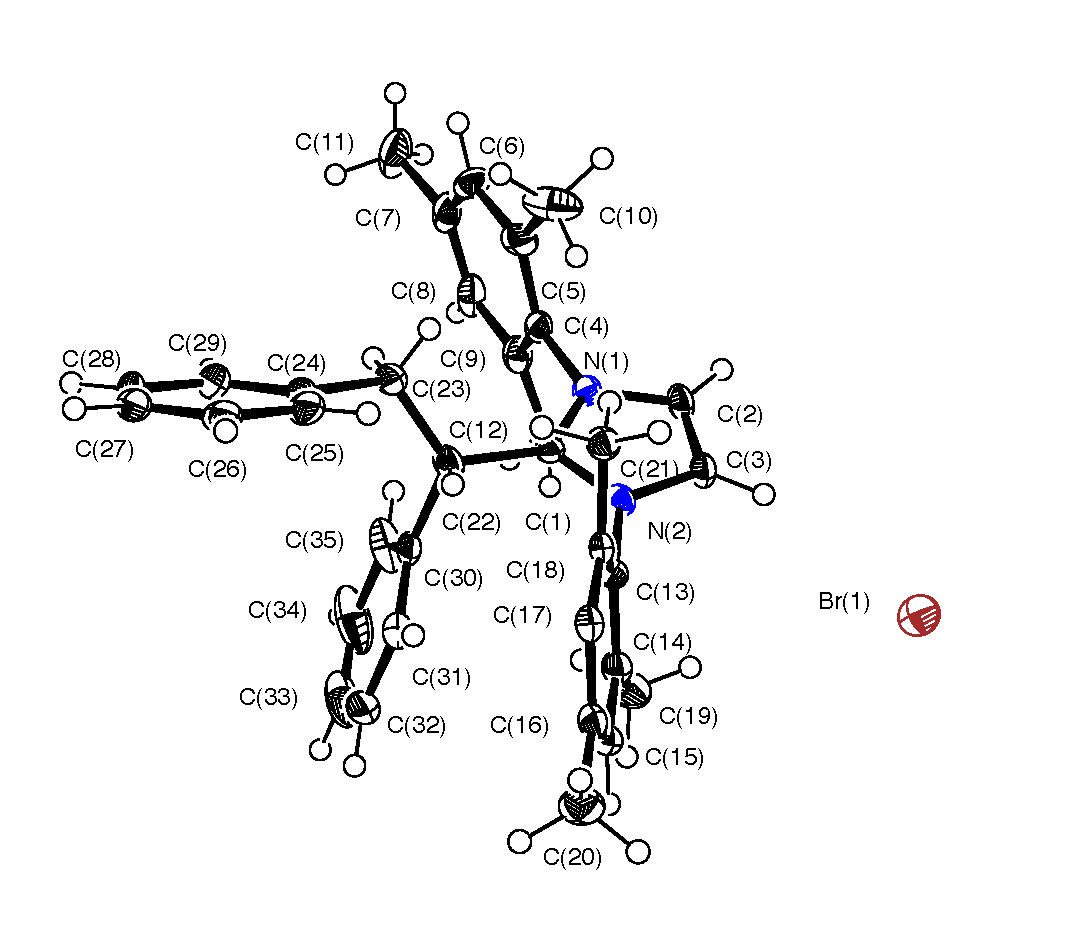
\includegraphics[width=6in]{chp_alkylation/images/xray/xcaf_labelled}
    \begin{textblock}{1}(14,-15)
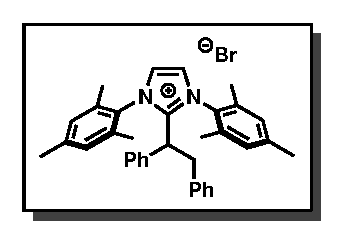
\includegraphics[scale=0.8]{chp_alkylation/images/xcaf}
\end{textblock}
  \caption{ORTEP drawing of  imidazolium salt \ref{cmp:xcaf} shown at 50\% probability }
\end{figure}
\pagebreak
\begin{table}[h]
\centering
\caption{Crystal data and structure refinement for \ref{cmp:xcaf}} 
\begin{tabular}{ll} 
\toprule
Empirical formula& 	\ce{C37H43BrCl4N2O} \\
Formula weight&	753.44 \\
Temperature &	100(2) K \\
Wavelength& 	0.71073 \AA  \\
Crystal system& 	Triclinic \\
Space group& 	P $-$1 \\
Unit cell dimensions&	a = 11.8192(9)  \AA\ $\alpha$ = 112.692(5)$^\circ$. \\
	&b = 11.9317(10)  \AA\	$\beta$ = 93.816(5)$^\circ$. \\
	&c = 14.5923(12)  \AA\	$\gamma$ = 96.976(5)$^\circ$. \\
Volume&	1870.0(3) \AA$^3$ \\
Z&	2 \\
Density (calculated)&	1.336 Mg/m$^3$ \\
Absorption coefficient&	1.416 mm$^{-1}$ \\
F(000) &	780 \\
Crystal size &	0.17 x 0.08 x 0.05 mm$^3$ \\
Theta range for data collection &	1.52 to 28.71$^\circ$. \\
Index ranges &	$-$15$<=$h$<=$15, $-$15$<=$k$<=$16, $-$19$<=$l$<=$19 \\
Reflections collected &	31263 \\
Independent reflections &	9546 [R(int) = 0.0462] \\
Completeness to theta = 28.71$^\circ$ &	98.8\% \\ 
Absorption correction&	Semi-empirical from equivalents \\
Max. and min. transmission &	0.9377 and 0.7938 \\
Refinement method	&Full-matrix least-squares on F$^2$ \\
Data / restraints / parameters &	 9546 / 345 / 489 \\
Goodness-of-fit on F$^2$ & 	1.020 \\
Final R indices [I$>$2sigma(I)] &	R1 = 0.0610, wR2 = 0.1381 \\
R indices (all data) &	R1 = 0.1000, wR2 = 0.1534 \\
Extinction coefficient	& na \\
Largest diff. peak and hole &	0.735 and $-$0.677 e.\AA$^{-3}$ \\
\bottomrule
\end{tabular}
\end{table}

\twocolumn
\begin{center}
\tablefirsthead{%
\toprule
&x&y&z&U(eq) \\
\midrule}
\tablehead{%
\multicolumn{5}{c}{\footnotesize \textbf{Table \thetable} continued\ldots} \\
\toprule
&x&y&z&U(eq) \\
\midrule
}
\tabletail{%
%\midrule
\multicolumn{5}{c}{\small \ldots}\\
}
\tablelasttail{\bottomrule} 
\topcaption{Atomic coordinates (x 10$^4$) and equivalent isotropic displacement
parameters (\AA$^2$x 10$^3$) for \ref{cmp:xcaf}} {\footnotesize \singlespacing
\begin{supertabular}{lcccc}
Br(1)&1403(1)&4925(1)&3543(1)&35(1)\\
N(1)&2069(2)&3995(2)&7185(2)&19(1)\\
N(2)&2968(2)&3639(2)&5887(2)&19(1)\\
C(1)&2863(2)&3370(3)&6696(2)&19(1)\\
C(2)&1668(3)&4669(3)&6679(2)&24(1)\\
C(3)&2228(3)&4445(3)&5867(2)&22(1)\\
C(4)&1643(3)&3968(3)&8084(2)&22(1)\\
C(5)&2215(3)&4780(3)&9013(2)&29(1)\\
C(6)&1799(3)&4708(3)&9862(2)&34(1)\\
C(7)&853(3)&3861(4)&9785(3)&35(1)\\
C(8)&275(3)&3120(3)&8848(3)&31(1)\\
C(9)&648(3)&3156(3)&7976(3)&26(1)\\
C(10)&3220(3)&5749(4)&9120(3)&46(1)\\
C(11)&431(4)&3765(4)&10714(3)&51(1)\\
C(12)&$-$35(3)&2407(3)&6968(3)&34(1)\\
C(13)&3757(3)&3191(3)&5159(2)&19(1)\\
C(14)&3329(3)&2233(3)&4234(2)&23(1)\\
C(15)&4106(3)&1801(3)&3567(2)&26(1)\\
C(16)&5277(3)&2294(3)&3792(2)&25(1)\\
C(17)&5652(3)&3244(3)&4718(2)&21(1)\\
C(18)&4906(3)&3726(3)&5410(2)&19(1)\\
C(19)&2069(3)&1678(3)&3976(3)&33(1)\\
C(20)&6101(3)&1805(4)&3040(3)&35(1)\\
C(21)&5341(3)&4804(3)&6383(2)&22(1)\\
C(22)&3517(3)&2506(3)&6959(3)&33(1)\\
C(23)&3960(4)&2866(5)&8007(4)&25(1)\\
C(24)&4981(7)&2274(10)&8171(8)&23(1)\\
C(25)&6041(4)&2601(5)&7901(4)&29(1)\\
C(26)&6998(5)&2123(5)&8085(4)&32(1)\\
C(27)&6917(7)&1349(11)&8579(9)&36(2)\\
C(28)&5889(7)&1021(8)&8858(6)&36(2)\\
C(29)&4915(5)&1493(5)&8670(5)&30(1)\\
C(23X)&4639(7)&2872(7)&7474(6)&19(2)\\
C(24X)&5119(11)&2170(20)&8049(15)&25(2)\\
C(25X)&6235(9)&1938(9)&7981(7)&28(2)\\
C(26X)&6692(13)&1290(20)&8496(17)&37(2)\\
C(27X)&6039(11)&921(15)&9099(10)&35(2)\\
C(28X)&4911(9)&1108(8)&9156(7)&34(2)\\
C(29X)&4467(9)&1731(10)&8624(8)&29(2)\\
C(30)&3076(3)&1169(3)&6293(2)&22(1)\\
C(31)&3629(3)&539(3)&5492(3)&32(1)\\
C(32)&3192(4)&$-$683(4)&4884(3)&51(1)\\
C(33)&2211(4)&$-$1249(4)&5086(4)&64(1)\\
C(34)&1677(4)&$-$624(4)&5876(5)&62(1)\\
C(35)&2102(3)&575(4)&6478(3)&41(1)\\
C(1S)&6967(4)&7179(4)&8291(3)&45(1)\\
Cl(1S)&6236(2)&6470(2)&9003(1)&64(1)\\
Cl(2S)&7783(3)&8619(2)&9004(2)&71(1)\\
Cl(1T)&5987(11)&7059(16)&8942(8)&64(1)\\
Cl(2T)&7830(30)&8500(20)&9244(18)&71(1)\\
C(2S)&688(5)&8523(4)&8044(3)&59(1)\\
Cl(3S)&1818(1)&8408(1)&8821(1)&61(1)\\
Cl(4S)&450(1)&10069(1)&8408(1)&61(1)\\
O(1)&9368(3)&3347(2)&4223(2)&42(1)\\
\end{supertabular}
}
\singlespacing{\noindent \footnotesize U(eq) is defined as one third of  the trace of the
\\orthogonalized U$^{ij}$ tensor.}
\end{center}


\begin{center}
\tablefirsthead{%
\toprule}
\tablehead{%
\multicolumn{2}{c}{\footnotesize \textbf{Table \thetable} continued\ldots} \\
\toprule
}
\tabletail{%
%\midrule
\multicolumn{2}{c}{\small \ldots}\\
}
\tablelasttail{\bottomrule}
\topcaption{Bond lengths (\AA) and angles (${^\circ}$) for \ref{cmp:xcaf}}
{\footnotesize \singlespacing
\begin{supertabular}{p{1.5in}c}
N(1)-C(1) &1.340(4)\\
N(1)-C(2) &1.386(4)\\
N(1)-C(4) &1.447(4)\\
N(2)-C(1) &1.347(4)\\
N(2)-C(3) &1.383(4)\\
N(2)-C(13) &1.448(4)\\
C(1)-C(22) &1.505(4)\\
C(2)-C(3) &1.348(5)\\
C(2)-H(2A) &0.95\\
C(3)-H(3A) &0.95\\
C(4)-C(9) &1.388(4)\\
C(4)-C(5) &1.392(4)\\
C(5)-C(6) &1.392(5)\\
C(5)-C(10) &1.509(5)\\
C(6)-C(7) &1.381(6)\\
C(6)-H(6A) &0.95\\
C(7)-C(8) &1.382(5)\\
C(7)-C(11) &1.514(5)\\
C(8)-C(9) &1.389(5)\\
C(8)-H(8A) &0.95\\
C(9)-C(12) &1.505(5)\\
C(10)-H(10A) &0.98\\
C(10)-H(10B) &0.98\\
C(10)-H(10C) &0.98\\
C(11)-H(11A) &0.98\\
C(11)-H(11B) &0.98\\
C(11)-H(11C) &0.98\\
C(12)-H(12A) &0.98\\
C(12)-H(12B) &0.98\\
C(12)-H(12C) &0.98\\
C(13)-C(18) &1.389(4)\\
C(13)-C(14) &1.401(4)\\
C(14)-C(15) &1.380(5)\\
C(14)-C(19) &1.514(4)\\
C(15)-C(16) &1.400(5)\\
C(15)-H(15A) &0.95\\
C(16)-C(17) &1.387(4)\\
C(16)-C(20) &1.510(5)\\
C(17)-C(18) &1.386(4)\\
C(17)-H(17A) &0.95\\
C(18)-C(21) &1.506(4)\\
C(19)-H(19A) &0.98\\
C(19)-H(19B) &0.98\\
C(19)-H(19C) &0.98\\
C(20)-H(20A) &0.98\\
C(20)-H(20B) &0.98\\
C(20)-H(20C) &0.98\\
C(21)-H(21A) &0.98\\
C(21)-H(21B) &0.98\\
C(21)-H(21C) &0.98\\
C(22)-C(23X) &1.410(8)\\
C(22)-C(23) &1.460(6)\\
C(22)-C(30) &1.515(4)\\
C(22)-H(22) &1\\
C(23)-C(24) &1.520(7)\\
C(23)-H(23A) &0.99\\
C(23)-H(23B) &0.99\\
C(24)-C(29) &1.385(8)\\
C(24)-C(25) &1.394(8)\\
C(25)-C(26) &1.382(7)\\
C(25)-H(25A) &0.95\\
C(26)-C(27) &1.373(10)\\
C(26)-H(26A) &0.95\\
C(27)-C(28) &1.367(9)\\
C(27)-H(27A) &0.95\\
C(28)-C(29) &1.397(9)\\
C(28)-H(28A) &0.95\\
C(29)-H(29A) &0.95\\
C(23X)-C(24X) &1.521(12)\\
C(23X)-H(23C) &0.99\\
C(23X)-H(23D) &0.99\\
C(24X)-C(29X) &1.379(12)\\
C(24X)-C(25X) &1.383(11)\\
C(25X)-C(26X) &1.393(14)\\
C(25X)-H(25B) &0.95\\
C(26X)-C(27X) &1.371(13)\\
C(26X)-H(26B) &0.95\\
C(27X)-C(28X) &1.381(13)\\
C(27X)-H(27B) &0.95\\
C(28X)-C(29X) &1.384(11)\\
C(28X)-H(28B) &0.95\\
C(29X)-H(29B) &0.95\\
C(30)-C(35) &1.376(5)\\
C(30)-C(31) &1.379(5)\\
C(31)-C(32) &1.392(5)\\
C(31)-H(31A) &0.95\\
C(32)-C(33) &1.377(7)\\
C(32)-H(32A) &0.95\\
C(33)-C(34) &1.353(8)\\
C(33)-H(33A) &0.95\\
C(34)-C(35) &1.367(6)\\
C(34)-H(34A) &0.95\\
C(35)-H(35A) &0.95\\
C(1S)-Cl(1T) &1.573(13)\\
C(1S)-Cl(2S) &1.747(5)\\
C(1S)-Cl(1S) &1.778(5)\\
C(1S)-Cl(2T) &1.79(2)\\
C(1S)-H(1S1) &0.99\\
C(1S)-H(1S2) &0.99\\
C(2S)-Cl(3S) &1.747(5)\\
C(2S)-Cl(4S) &1.776(5)\\
C(2S)-H(2S1) &0.99\\
C(2S)-H(2S2) &0.99\\
O(1)-H(1O) &0.808(19)\\
O(1)-H(2O) &0.816(19)\\
C(1)-N(1)-C(2)&109.5(3)\\
C(1)-N(1)-C(4)&126.9(3)\\
C(2)-N(1)-C(4)&123.5(3)\\
C(1)-N(2)-C(3)&109.7(3)\\
C(1)-N(2)-C(13)&125.7(2)\\
C(3)-N(2)-C(13)&124.5(3)\\
N(1)-C(1)-N(2)&106.8(3)\\
N(1)-C(1)-C(22)&128.2(3)\\
N(2)-C(1)-C(22)&125.0(3)\\
C(3)-C(2)-N(1)&107.2(3)\\
C(3)-C(2)-H(2A)&126.4\\
N(1)-C(2)-H(2A)&126.4\\
C(2)-C(3)-N(2)&106.8(3)\\
C(2)-C(3)-H(3A)&126.6\\
N(2)-C(3)-H(3A)&126.6\\
C(9)-C(4)-C(5)&123.0(3)\\
C(9)-C(4)-N(1)&117.9(3)\\
C(5)-C(4)-N(1)&119.1(3)\\
C(6)-C(5)-C(4)&117.6(3)\\
C(6)-C(5)-C(10)&120.0(3)\\
C(4)-C(5)-C(10)&122.3(3)\\
C(7)-C(6)-C(5)&121.1(3)\\
C(7)-C(6)-H(6A)&119.4\\
C(5)-C(6)-H(6A)&119.4\\
C(6)-C(7)-C(8)&119.1(3)\\
C(6)-C(7)-C(11)&120.6(4)\\
C(8)-C(7)-C(11)&120.3(4)\\
C(7)-C(8)-C(9)&122.2(3)\\
C(7)-C(8)-H(8A)&118.9\\
C(9)-C(8)-H(8A)&118.9\\
C(4)-C(9)-C(8)&116.8(3)\\
C(4)-C(9)-C(12)&121.7(3)\\
C(8)-C(9)-C(12)&121.5(3)\\
C(5)-C(10)-H(10A)&109.5\\
C(5)-C(10)-H(10B)&109.5\\
H(10A)-C(10)-H(10B)&109.5\\
C(5)-C(10)-H(10C)&109.5\\
H(10A)-C(10)-H(10C)&109.5\\
H(10B)-C(10)-H(10C)&109.5\\
C(7)-C(11)-H(11A)&109.5\\
C(7)-C(11)-H(11B)&109.5\\
H(11A)-C(11)-H(11B)&109.5\\
C(7)-C(11)-H(11C)&109.5\\
H(11A)-C(11)-H(11C)&109.5\\
H(11B)-C(11)-H(11C)&109.5\\
C(9)-C(12)-H(12A)&109.5\\
C(9)-C(12)-H(12B)&109.5\\
H(12A)-C(12)-H(12B)&109.5\\
C(9)-C(12)-H(12C)&109.5\\
H(12A)-C(12)-H(12C)&109.5\\
H(12B)-C(12)-H(12C)&109.5\\
C(18)-C(13)-C(14)&122.8(3)\\
C(18)-C(13)-N(2)&118.6(2)\\
C(14)-C(13)-N(2)&118.6(3)\\
C(15)-C(14)-C(13)&117.3(3)\\
C(15)-C(14)-C(19)&121.0(3)\\
C(13)-C(14)-C(19)&121.6(3)\\
C(14)-C(15)-C(16)&122.0(3)\\
C(14)-C(15)-H(15A)&119\\
C(16)-C(15)-H(15A)&119\\
C(17)-C(16)-C(15)&118.2(3)\\
C(17)-C(16)-C(20)&121.2(3)\\
C(15)-C(16)-C(20)&120.6(3)\\
C(18)-C(17)-C(16)&122.2(3)\\
C(18)-C(17)-H(17A)&118.9\\
C(16)-C(17)-H(17A)&118.9\\
C(17)-C(18)-C(13)&117.5(3)\\
C(17)-C(18)-C(21)&120.3(3)\\
C(13)-C(18)-C(21)&122.2(3)\\
C(14)-C(19)-H(19A)&109.5\\
C(14)-C(19)-H(19B)&109.5\\
H(19A)-C(19)-H(19B)&109.5\\
C(14)-C(19)-H(19C)&109.5\\
H(19A)-C(19)-H(19C)&109.5\\
H(19B)-C(19)-H(19C)&109.5\\
C(16)-C(20)-H(20A)&109.5\\
C(16)-C(20)-H(20B)&109.5\\
H(20A)-C(20)-H(20B)&109.5\\
C(16)-C(20)-H(20C)&109.5\\
H(20A)-C(20)-H(20C)&109.5\\
H(20B)-C(20)-H(20C)&109.5\\
C(18)-C(21)-H(21A)&109.5\\
C(18)-C(21)-H(21B)&109.5\\
H(21A)-C(21)-H(21B)&109.5\\
C(18)-C(21)-H(21C)&109.5\\
H(21A)-C(21)-H(21C)&109.5\\
H(21B)-C(21)-H(21C)&109.5\\
C(23X)-C(22)-C(23)&47.4(4)\\
C(23X)-C(22)-C(1)&122.9(4)\\
C(23)-C(22)-C(1)&117.9(3)\\
C(23X)-C(22)-C(30)&120.8(4)\\
C(23)-C(22)-C(30)&120.6(3)\\
C(1)-C(22)-C(30)&112.4(2)\\
C(23X)-C(22)-H(22)&52.8\\
C(23)-C(22)-H(22)&100.2\\
C(1)-C(22)-H(22)&100.2\\
C(30)-C(22)-H(22)&100.2\\
C(22)-C(23)-C(24)&114.5(5)\\
C(22)-C(23)-H(23A)&108.6\\
C(24)-C(23)-H(23A)&108.6\\
C(22)-C(23)-H(23B)&108.6\\
C(24)-C(23)-H(23B)&108.6\\
H(23A)-C(23)-H(23B)&107.6\\
C(29)-C(24)-C(25)&118.3(6)\\
C(29)-C(24)-C(23)&121.4(6)\\
C(25)-C(24)-C(23)&120.1(6)\\
C(26)-C(25)-C(24)&121.4(6)\\
C(26)-C(25)-H(25A)&119.3\\
C(24)-C(25)-H(25A)&119.3\\
C(27)-C(26)-C(25)&119.5(6)\\
C(27)-C(26)-H(26A)&120.3\\
C(25)-C(26)-H(26A)&120.3\\
C(28)-C(27)-C(26)&120.2(8)\\
C(28)-C(27)-H(27A)&119.9\\
C(26)-C(27)-H(27A)&119.9\\
C(27)-C(28)-C(29)&120.7(7)\\
C(27)-C(28)-H(28A)&119.7\\
C(29)-C(28)-H(28A)&119.7\\
C(24)-C(29)-C(28)&119.9(6)\\
C(24)-C(29)-H(29A)&120.1\\
C(28)-C(29)-H(29A)&120.1\\
C(22)-C(23X)-C(24X)&121.6(9)\\
C(22)-C(23X)-H(23C)&106.9\\
C(24X)-C(23X)-H(23C)&106.9\\
C(22)-C(23X)-H(23D)&106.9\\
C(24X)-C(23X)-H(23D)&106.9\\
H(23C)-C(23X)-H(23D)&106.7\\
C(29X)-C(24X)-C(25X)&118.2(10)\\
C(29X)-C(24X)-C(23X)&122.1(9)\\
C(25X)-C(24X)-C(23X)&119.6(10)\\
C(24X)-C(25X)-C(26X)&120.7(11)\\
C(24X)-C(25X)-H(25B)&119.6\\
C(26X)-C(25X)-H(25B)&119.6\\
C(27X)-C(26X)-C(25X)&119.5(13)\\
C(27X)-C(26X)-H(26B)&120.2\\
C(25X)-C(26X)-H(26B)&120.2\\
C(26X)-C(27X)-C(28X)&120.9(12)\\
C(26X)-C(27X)-H(27B)&119.6\\
C(28X)-C(27X)-H(27B)&119.6\\
C(27X)-C(28X)-C(29X)&118.5(10)\\
C(27X)-C(28X)-H(28B)&120.7\\
C(29X)-C(28X)-H(28B)&120.7\\
C(24X)-C(29X)-C(28X)&122.0(10)\\
C(24X)-C(29X)-H(29B)&119\\
C(28X)-C(29X)-H(29B)&119\\
C(35)-C(30)-C(31)&119.2(3)\\
C(35)-C(30)-C(22)&119.8(3)\\
C(31)-C(30)-C(22)&121.0(3)\\
C(30)-C(31)-C(32)&119.6(4)\\
C(30)-C(31)-H(31A)&120.2\\
C(32)-C(31)-H(31A)&120.2\\
C(33)-C(32)-C(31)&119.7(4)\\
C(33)-C(32)-H(32A)&120.2\\
C(31)-C(32)-H(32A)&120.2\\
C(34)-C(33)-C(32)&120.2(4)\\
C(34)-C(33)-H(33A)&119.9\\
C(32)-C(33)-H(33A)&119.9\\
C(33)-C(34)-C(35)&120.4(4)\\
C(33)-C(34)-H(34A)&119.8\\
C(35)-C(34)-H(34A)&119.8\\
C(34)-C(35)-C(30)&120.8(4)\\
C(34)-C(35)-H(35A)&119.6\\
C(30)-C(35)-H(35A)&119.6\\
Cl(1T)-C(1S)-Cl(2S)&104.1(6)\\
Cl(1T)-C(1S)-Cl(1S)&27.7(7)\\
Cl(2S)-C(1S)-Cl(1S)&114.4(3)\\
Cl(1T)-C(1S)-Cl(2T)&96.2(12)\\
Cl(2S)-C(1S)-Cl(2T)&13.8(8)\\
Cl(1S)-C(1S)-Cl(2T)&102.2(10)\\
Cl(1T)-C(1S)-H(1S1)&135.2\\
Cl(2S)-C(1S)-H(1S1)&108.6\\
Cl(1S)-C(1S)-H(1S1)&108.6\\
Cl(2T)-C(1S)-H(1S1)&108.7\\
Cl(1T)-C(1S)-H(1S2)&89.4\\
Cl(2S)-C(1S)-H(1S2)&108.6\\
Cl(1S)-C(1S)-H(1S2)&108.6\\
Cl(2T)-C(1S)-H(1S2)&120.5\\
H(1S1)-C(1S)-H(1S2)&107.6\\
Cl(3S)-C(2S)-Cl(4S)&111.5(2)\\
Cl(3S)-C(2S)-H(2S1)&109.3\\
Cl(4S)-C(2S)-H(2S1)&109.3\\
Cl(3S)-C(2S)-H(2S2)&109.3\\
Cl(4S)-C(2S)-H(2S2)&109.3\\
H(2S1)-C(2S)-H(2S2)&108\\
H(1O)-O(1)-H(2O)&100(5)\\
\end{supertabular}
}
\end{center}

\begin{center}
\tablefirsthead{%
\toprule
&x&y&z&U(eq) \\
\midrule}
\tablehead{%
\multicolumn{5}{c}{\footnotesize \textbf{Table \thetable} continued\ldots} \\
\toprule
&x&y&z&U(eq) \\
\midrule
}
\tabletail{%
%\midrule
\multicolumn{5}{c}{\small \ldots}\\
}
\tablelasttail{\bottomrule}
\topcaption{Hydrogen coordinates (x 10$^4$) and isotropic displacement parameters (\AA$^2$x 10$^3$)
for \ref{cmp:xcaf}} {\footnotesize \singlespacing
\begin{supertabular}{lcccc}
H(2A)&1103&5191&6868&28\\
H(3A)&2134&4778&5376&26\\
H(6A)&2173&5251&10505&40\\
H(8A)&$-$399&2568&8800&37\\
H(10A)&3483&5588&8464&69\\
H(10B)&3847&5726&9583&69\\
H(10C)&2983&6562&9381&69\\
H(11A)&605&3003&10756&77\\
H(11B)&$-$401&3759&10678&77\\
H(11C)&816&4472&11308&77\\
H(12A)&$-$474&1664&6982&50\\
H(12B)&489&2174&6457&50\\
H(12C)&$-$564&2897&6809&50\\
H(15A)&3838&1151&2935&31\\
H(17A)&6447&3576&4883&26\\
H(19A)&1948&991&3318&50\\
H(19B)&1614&2306&3961&50\\
H(19C)&1830&1378&4483&50\\
H(20A)&6859&2317&3288&53\\
H(20B)&5818&1826&2401&53\\
H(20C)&6161&956&2943&53\\
H(21A)&5951&4594&6747&33\\
H(21B)&4709&5003&6790&33\\
H(21C)&5646&5517&6246&33\\
H(22)&4248&2631&6678&40\\
H(23A)&3333&2649&8356&30\\
H(23B)&4188&3772&8319&30\\
H(25A)&6108&3164&7585&35\\
H(26A)&7706&2329&7872&38\\
H(27A)&7578&1039&8728&43\\
H(28A)&5836&467&9184&43\\
H(29A)&4209&1278&8883&36\\
H(23C)&4690&3735&7956&23\\
H(23D)&5169&2878&6978&23\\
H(25B)&6694&2220&7579&34\\
H(26B)&7451&1116&8430&44\\
H(27B)&6367&528&9484&42\\
H(28B)&4450&816&9552&40\\
H(29B)&3690&1858&8655&34\\
H(31A)&4305&935&5357&38\\
H(32A)&3569&$-$1125&4331&61\\
H(33A)&1907&$-$2081&4669&76\\
H(34A)&1002&$-$1022&6012&74\\
H(35A)&1720&1003&7031&50\\
H(1S1)&7479&6627&7900&54\\
H(1S2)&6393&7272&7810&54\\
H(2S1)&$-$21&8008&8073&71\\
H(2S2)&866&8205&7344&71\\
H(1O)&9940(30)&3750(40)&4160(40)&62\\
H(2O)&9320(40)&3730(40)&4814(17)&62\\
\end{supertabular}
}
\end{center}

\pagebreak
\begin{center}
\tablefirsthead{%
\toprule}
\tablehead{%
\multicolumn{2}{c}{\footnotesize \textbf{Table \thetable} continued\ldots} \\
\toprule
}
\tabletail{%
%\midrule
\multicolumn{2}{c}{\small \ldots}\\
}
\tablelasttail{\bottomrule}
\topcaption{Torsion angles ($^{\circ}$) for \ref{cmp:xcaf}}
{\footnotesize \singlespacing
\begin{supertabular}{p{1.8in}c}
C(2)-N(1)-C(1)-N(2)&0.0(3)\\
C(4)-N(1)-C(1)-N(2)&178.0(3)\\
C(2)-N(1)-C(1)-C(22)&$-$179.0(3)\\
C(4)-N(1)-C(1)-C(22)&$-$1.0(5)\\
C(3)-N(2)-C(1)-N(1)&$-$0.1(3)\\
C(13)-N(2)-C(1)-N(1)&178.2(2)\\
C(3)-N(2)-C(1)-C(22)&179.0(3)\\
C(13)-N(2)-C(1)-C(22)&$-$2.8(4)\\
C(1)-N(1)-C(2)-C(3)&0.1(3)\\
C(4)-N(1)-C(2)-C(3)&$-$178.0(3)\\
N(1)-C(2)-C(3)-N(2)&$-$0.1(3)\\
C(1)-N(2)-C(3)-C(2)&0.1(3)\\
C(13)-N(2)-C(3)-C(2)&$-$178.1(3)\\
C(1)-N(1)-C(4)-C(9)&$-$94.3(4)\\
C(2)-N(1)-C(4)-C(9)&83.5(4)\\
C(1)-N(1)-C(4)-C(5)&88.0(4)\\
C(2)-N(1)-C(4)-C(5)&$-$94.2(4)\\
C(9)-C(4)-C(5)-C(6)&4.0(5)\\
N(1)-C(4)-C(5)-C(6)&$-$178.4(3)\\
C(9)-C(4)-C(5)-C(10)&$-$173.3(3)\\
N(1)-C(4)-C(5)-C(10)&4.3(5)\\
C(4)-C(5)-C(6)-C(7)&0.0(5)\\
C(10)-C(5)-C(6)-C(7)&177.4(3)\\
C(5)-C(6)-C(7)-C(8)&$-$3.5(5)\\
C(5)-C(6)-C(7)-C(11)&178.1(3)\\
C(6)-C(7)-C(8)-C(9)&3.2(5)\\
C(11)-C(7)-C(8)-C(9)&$-$178.4(3)\\
C(5)-C(4)-C(9)-C(8)&$-$4.3(5)\\
N(1)-C(4)-C(9)-C(8)&178.1(3)\\
C(5)-C(4)-C(9)-C(12)&172.0(3)\\
N(1)-C(4)-C(9)-C(12)&$-$5.6(4)\\
C(7)-C(8)-C(9)-C(4)&0.6(5)\\
C(7)-C(8)-C(9)-C(12)&$-$175.7(3)\\
C(1)-N(2)-C(13)-C(18)&$-$77.2(4)\\
C(3)-N(2)-C(13)-C(18)&100.7(3)\\
C(1)-N(2)-C(13)-C(14)&102.4(3)\\
C(3)-N(2)-C(13)-C(14)&$-$79.6(4)\\
C(18)-C(13)-C(14)-C(15)&1.4(5)\\
N(2)-C(13)-C(14)-C(15)&$-$178.2(3)\\
C(18)-C(13)-C(14)-C(19)&$-$179.2(3)\\
N(2)-C(13)-C(14)-C(19)&1.1(5)\\
C(13)-C(14)-C(15)-C(16)&$-$0.1(5)\\
C(19)-C(14)-C(15)-C(16)&$-$179.5(3)\\
C(14)-C(15)-C(16)-C(17)&0.0(5)\\
C(14)-C(15)-C(16)-C(20)&$-$179.5(3)\\
C(15)-C(16)-C(17)-C(18)&$-$1.1(5)\\
C(20)-C(16)-C(17)-C(18)&178.4(3)\\
C(16)-C(17)-C(18)-C(13)&2.2(4)\\
C(16)-C(17)-C(18)-C(21)&$-$176.6(3)\\
C(14)-C(13)-C(18)-C(17)&$-$2.4(5)\\
N(2)-C(13)-C(18)-C(17)&177.2(3)\\
C(14)-C(13)-C(18)-C(21)&176.4(3)\\
N(2)-C(13)-C(18)-C(21)&$-$4.0(4)\\
N(1)-C(1)-C(22)-C(23X)&$-$97.9(6)\\
N(2)-C(1)-C(22)-C(23X)&83.3(6)\\
N(1)-C(1)-C(22)-C(23)&$-$42.6(5)\\
N(2)-C(1)-C(22)-C(23)&138.6(4)\\
N(1)-C(1)-C(22)-C(30)&104.5(4)\\
N(2)-C(1)-C(22)-C(30)&$-$74.3(4)\\
C(23X)-C(22)-C(23)-C(24)&$-$45.7(6)\\
C(1)-C(22)-C(23)-C(24)&$-$156.1(5)\\
C(30)-C(22)-C(23)-C(24)&59.6(6)\\
C(22)-C(23)-C(24)-C(29)&$-$116.9(9)\\
C(22)-C(23)-C(24)-C(25)&69.1(10)\\
C(29)-C(24)-C(25)-C(26)&2.7(13)\\
C(23)-C(24)-C(25)-C(26)&176.8(6)\\
C(24)-C(25)-C(26)-C(27)&$-$2.6(11)\\
C(25)-C(26)-C(27)-C(28)&2.1(15)\\
C(26)-C(27)-C(28)-C(29)&$-$1.7(17)\\
C(25)-C(24)-C(29)-C(28)&$-$2.2(13)\\
C(23)-C(24)-C(29)-C(28)&$-$176.3(7)\\
C(27)-C(28)-C(29)-C(24)&1.8(14)\\
C(23)-C(22)-C(23X)-C(24X)&58.6(10)\\
C(1)-C(22)-C(23X)-C(24X)&157.9(10)\\
C(30)-C(22)-C(23X)-C(24X)&$-$46.3(12)\\
C(22)-C(23X)-C(24X)-C(29X)&$-$41(2)\\
C(22)-C(23X)-C(24X)-C(25X)&137.4(14)\\
C(29X)-C(24X)-C(25X)-C(26X)&$-$1(3)\\
C(23X)-C(24X)-C(25X)-C(26X)&$-$179.7(17)\\
C(24X)-C(25X)-C(26X)-C(27X)&$-$2(3)\\
C(25X)-C(26X)-C(27X)-C(28X)&4(3)\\
C(26X)-C(27X)-C(28X)-C(29X)&$-$3(2)\\
C(25X)-C(24X)-C(29X)-C(28X)&2(3)\\
C(23X)-C(24X)-C(29X)-C(28X)&$-$179.2(13)\\
C(27X)-C(28X)-C(29X)-C(24X)&0(2)\\
C(23X)-C(22)-C(30)-C(35)&122.2(5)\\
C(23)-C(22)-C(30)-C(35)&66.4(5)\\
C(1)-C(22)-C(30)-C(35)&$-$79.7(4)\\
C(23X)-C(22)-C(30)-C(31)&$-$58.7(6)\\
C(23)-C(22)-C(30)-C(31)&$-$114.5(4)\\
C(1)-C(22)-C(30)-C(31)&99.4(4)\\
C(35)-C(30)-C(31)-C(32)&0.3(5)\\
C(22)-C(30)-C(31)-C(32)&$-$178.8(3)\\
C(30)-C(31)-C(32)-C(33)&0.1(5)\\
C(31)-C(32)-C(33)-C(34)&$-$0.4(6)\\
C(32)-C(33)-C(34)-C(35)&0.3(7)\\
C(33)-C(34)-C(35)-C(30)&0.1(6)\\
C(31)-C(30)-C(35)-C(34)&$-$0.4(5)\\
C(22)-C(30)-C(35)-C(34)&178.7(3)\\
\end{supertabular}
}
\end{center}

\onecolumn
\begin{table}[h]
\centering
\caption{Hydrogen bonds (\AA\  and $^{\circ}$) for \ref{cmp:xcaf}}
{\footnotesize
\begin{tabular}{lcccc} 
\\
\toprule
\ce{D-H}\ldots A& d(\ce{D-H}) & d(H\ldots A) & d(D\ldots A) & \angle(DHA) \\
\midrule
O(1)\ce{-}H(1O)...Br(1)\#1&0.808(19)&2.53(2)&3.313(3)&165(5)\\
O(1)\ce{-}H(2O)...Br(1)\#2&0.816(19)&2.58(2)&3.372(3)&163(5)\\
\bottomrule \\
\multicolumn{5}{l}{Symmetry transformations used to generate equivalent atoms:} \\
\multicolumn{5}{l}{\#1 $x+1,y,z$} \\
\multicolumn{5}{l}{\#2 $-x+1,-y+1,-z+1$} \\
\end{tabular}
}
\end{table}



\begin{center}
\tablefirsthead{%
\toprule
& U$^{11}$ & U$^{22}$ & U$^{33}$ & U$^{23}$ & U$^{13}$ & U$^{12}$ \\
\midrule}
\tablehead{%
\multicolumn{7}{c}{\footnotesize \textbf{Table \thetable} continued\ldots} \\
\toprule
& U$^{11}$ & U$^{22}$ & U$^{33}$ & U$^{23}$ & U$^{13}$ & U$^{12}$ \\
\midrule
}
\tabletail{%
%\midrule
\multicolumn{7}{c}{\small \ldots}\\
}
\tablelasttail{\bottomrule}
\topcaption{Anisotropic displacement parameters (\AA$^2$x 10$^3$) for  \ref{cmp:xcaf}}
{\footnotesize \singlespacing
\begin{supertabular}{lcccccc}
Br(1)&28(1) &44(1)&34(1) &15(1)&3(1) &11(1)\\
N(1)&18(1) &22(1)&19(1) &8(1)&2(1) &7(1)\\
N(2)&16(1) &18(1)&23(1) &6(1)&0(1) &5(1)\\
C(1)&19(1) &18(1)&16(1) &3(1)&$-$1(1) &5(1)\\
C(2)&23(2) &23(2)&30(2) &14(1)&5(1) &12(1)\\
C(3)&22(2) &22(2)&25(2) &13(1)&3(1) &9(1)\\
C(4)&23(2) &26(2)&21(2) &11(1)&6(1) &13(1)\\
C(5)&28(2) &31(2)&26(2) &4(1)&4(1) &17(1)\\
C(6)&39(2) &46(2)&16(2) &6(2)&5(1) &26(2)\\
C(7)&43(2) &47(2)&30(2) &23(2)&17(2) &33(2)\\
C(8)&30(2) &39(2)&38(2) &26(2)&14(2) &17(2)\\
C(9)&22(2) &29(2)&32(2) &15(1)&5(1) &11(1)\\
C(10)&36(2) &40(2)&39(2) &$-$9(2)&2(2) &$-$1(2)\\
C(11)&69(3) &74(3)&39(2) &39(2)&27(2) &46(2)\\
C(12)&26(2) &39(2)&37(2) &18(2)&$-$1(2) &0(2)\\
C(13)&21(1) &20(1)&18(2) &7(1)&4(1) &7(1)\\
C(14)&24(2) &21(2)&23(2) &8(1)&0(1) &6(1)\\
C(15)&32(2) &21(2)&21(2) &4(1)&$-$3(1) &8(1)\\
C(16)&32(2) &25(2)&24(2) &12(1)&7(1) &15(1)\\
C(17)&22(2) &21(2)&25(2) &12(1)&2(1) &7(1)\\
C(18)&24(2) &17(1)&20(2) &10(1)&1(1) &7(1)\\
C(19)&26(2) &29(2)&34(2) &4(2)&$-$5(1) &3(1)\\
C(20)&35(2) &42(2)&28(2) &9(2)&10(2) &17(2)\\
C(21)&22(2) &20(2)&23(2) &8(1)&1(1) &3(1)\\
C(22)&38(2) &22(2)&33(2) &4(1)&$-$13(2) &14(1)\\
C(23)&28(2) &25(2)&22(2) &6(2)&2(2) &12(2)\\
C(24)&26(2) &21(3)&19(3) &5(2)&$-$3(2) &9(2)\\
C(25)&29(2) &34(3)&21(2) &6(2)&$-$2(2) &14(2)\\
C(26)&30(3) &36(3)&22(2) &1(2)&$-$5(2) &16(2)\\
C(27)&39(3) &33(3)&25(3) &$-$1(2)&$-$15(3) &20(3)\\
C(28)&52(3) &27(3)&25(3) &7(2)&$-$14(3) &16(2)\\
C(29)&34(3) &29(3)&25(3) &8(2)&$-$7(2) &10(2)\\
C(23X)&21(3) &20(3)&17(3) &8(3)&$-$3(3) &4(3)\\
C(24X)&31(3) &25(3)&19(3) &8(3)&$-$7(3) &7(3)\\
C(25X)&36(3) &26(3)&18(3) &3(3)&$-$8(3) &14(3)\\
C(26X)&41(4) &32(4)&27(4) &0(3)&$-$16(4) &18(4)\\
C(27X)&49(4) &25(4)&24(5) &4(3)&$-$21(4) &15(3)\\
C(28X)&49(4) &25(4)&25(4) &11(3)&$-$14(3) &8(3)\\
C(29X)&38(4) &27(4)&23(4) &13(3)&$-$8(3) &8(3)\\
C(30)&25(2) &20(1)&23(2) &11(1)&$-$3(1) &6(1)\\
C(31)&45(2) &29(2)&27(2) &14(1)&4(2) &15(2)\\
C(32)&85(3) &35(2)&27(2) &2(2)&$-$12(2) &33(2)\\
C(33)&73(3) &22(2)&78(3) &13(2)&$-$50(2) &$-$1(2)\\
C(34)&39(2) &35(2)&118(4) &44(2)&$-$14(2) &$-$4(2)\\
C(35)&33(2) &37(2)&70(3) &34(2)&11(2) &13(2)\\
C(1S)&50(2) &38(2)&39(2) &5(2)&$-$6(2) &14(2)\\
Cl(1S)&54(1) &92(2)&40(1) &22(1)&$-$4(1) &5(1)\\
Cl(2S)&83(1) &30(1)&76(2) &1(1)&$-$37(1) &16(1)\\
Cl(1T)&54(1) &92(2)&40(1) &22(1)&$-$4(1) &5(1)\\
Cl(2T)&83(1) &30(1)&76(2) &1(1)&$-$37(1) &16(1)\\
C(2S)&80(3) &42(2)&46(3) &12(2)&$-$8(2) &9(2)\\
Cl(3S)&58(1) &67(1)&55(1) &20(1)&7(1) &16(1)\\
Cl(4S)&87(1) &45(1)&48(1) &15(1)&9(1) &15(1)\\
O(1)&50(2) &26(1)&40(2) &6(1)&8(1) &$-$2(1)\\
\end{supertabular}
}
\end{center}

{ \footnotesize
The anisotropic displacement factor exponent takes the form: 
$-2\pi^2\left[ h^2a*^2U^{11} + ... + 2 h k a* b* U^{12} \right]$ }

\pagebreak
%%%%%%%%%%% End of X-Ray Data for xcaf %%%%%%%%%%%%%%%%%%%%

%%%%%%%%%%% Begin  X-Ray Data for xcai %%%%%%%%%%%%%%%%%%%%
\subsection{Structural Data for Imidazolium Salt \ref{cmp:xcai}}
Suitable crystals for X-ray analysis were obtained by slow diffusion of Et$_2$O into a \ce{CHCl3}
solution at room temperature in a dry box. 
\begin{figure}[h]
  \centering
  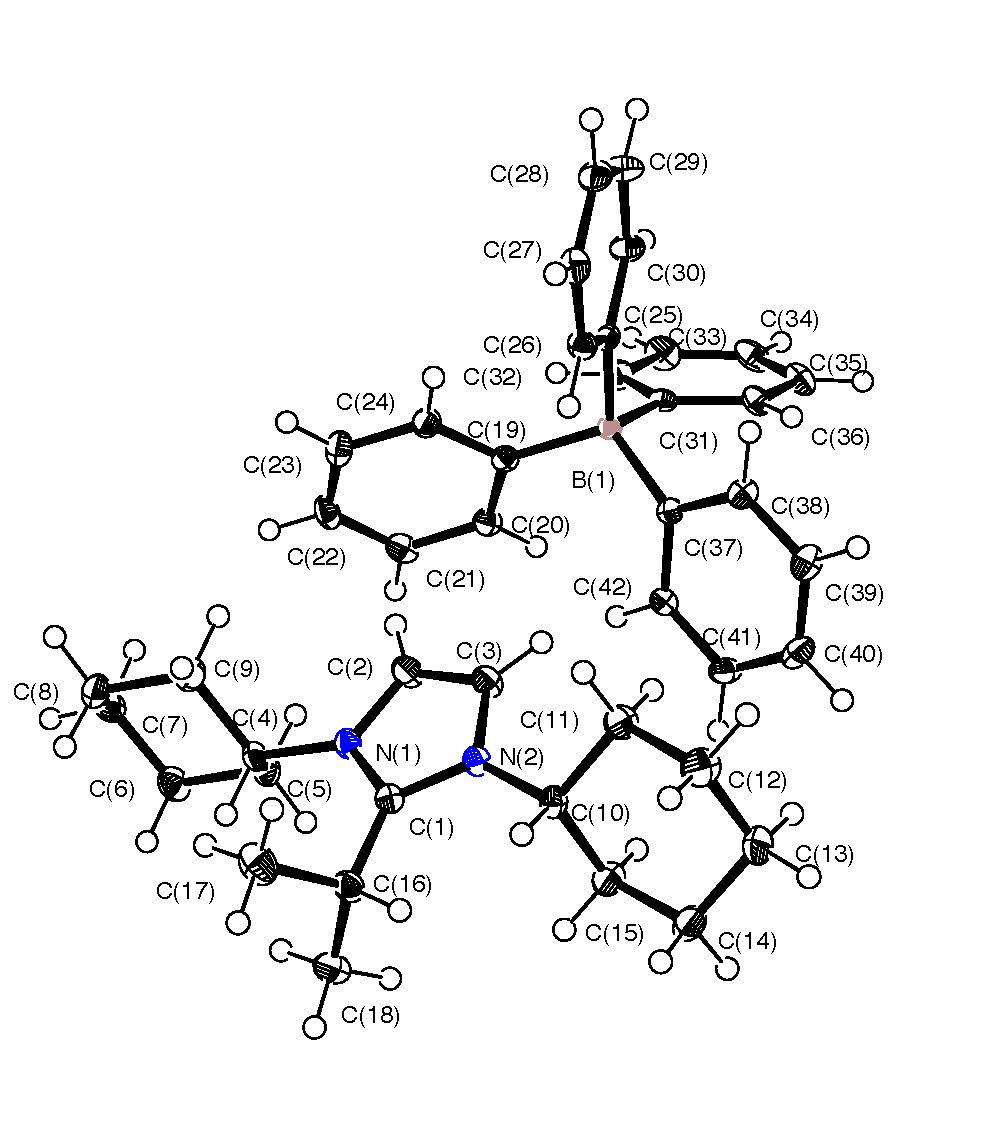
\includegraphics[width=5.2in]{chp_alkylation/images/xray/xcai_labelled}
    \begin{textblock}{1}(1,-17)
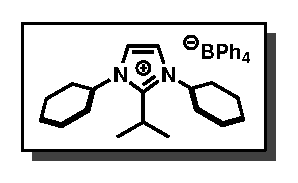
\includegraphics[scale=0.8]{chp_alkylation/images/xcai}
\end{textblock}
  \caption{ORTEP drawing of  imidazolium salt \ref{cmp:xcai} shown at 50\% probability }
\end{figure}

\pagebreak
\begin{table}[h]
\centering
\caption{Crystal data and structure refinement for \ref{cmp:xcai}} 
\begin{tabular}{ll} 
\toprule
Empirical formula& 	\ce{C43H53BCl2N2} \\
Formula weight&	679.58 \\
Temperature &	100(2) K \\
Wavelength& 	0.71073 \AA  \\
Crystal system& 	Orthorhombic \\
Space group& 	P2(1)2(1)2(1) \\
Unit cell dimensions&	a = 12.8426(8)   \AA\ $\alpha$ = 90$^\circ$. \\
	&b = 14.7152(9)  \AA\	$\beta$ = 90$^\circ$. \\
	&c = 19.9415(13)  \AA\	$\gamma$ = 90$^\circ$. \\
Volume&	3768.6(4) \AA$^3$ \\
Z&	4 \\
Density (calculated)&	1.198 Mg/m$^3$ \\
Absorption coefficient&	0.205 mm$^{-1}$ \\
F(000) &	1456 \\
Crystal size &	0.35 x 0.15 x 0.10 mm$^3$ \\
Theta range for data collection &	1.72 to 28.62$^\circ$. \\
Index ranges &	$-$17$<=$h$<=$17, $-$19$<=$k$<=$19, $-$26$<=$l$<=$26 \\
Reflections collected &	73941 \\
Independent reflections &	9632 [R(int) = 0.0452] \\
Completeness to theta = 28.62$^\circ$ &	99.7\% \\ 
Absorption correction&	Semi-empirical from equivalents \\
Max. and min. transmission &	0.9798 and 0.9318 \\
Refinement method	&Full-matrix least-squares on F$^2$ \\
Data / restraints / parameters &	 9632 / 0 / 433 \\
Goodness-of-fit on F$^2$ & 	1.028 \\
Final R indices [I$>$2sigma(I)] &	R1 = 0.0363, wR2 = 0.0899 \\
R indices (all data) &	R1 = 0.0422, wR2 = 0.0941 \\
Absolute structure parameter & 0.00(4) \\
Extinction coefficient	& na \\
Largest diff. peak and hole &	0.656 and $-$0.523 e.\AA$^{-3}$ \\
\bottomrule
\end{tabular}
\end{table}

\twocolumn
\begin{center}
\tablefirsthead{%
\toprule
&x&y&z&U(eq) \\
\midrule}
\tablehead{%
\multicolumn{5}{c}{\footnotesize \textbf{Table \thetable} continued\ldots} \\
\toprule
&x&y&z&U(eq) \\
\midrule
}
\tabletail{%
%\midrule
\multicolumn{5}{c}{\small \ldots}\\
}
\tablelasttail{\bottomrule} 
\topcaption{Atomic coordinates (x 10$^4$) and equivalent isotropic displacement
parameters (\AA$^2$x 10$^3$) for \ref{cmp:xcai}} {\footnotesize \singlespacing
\begin{supertabular}{lcccc}
N(1)&2437(1)&8450(1)&8609(1)&16(1)\\
N(2)&2153(1)&7643(1)&7720(1)&16(1)\\
B(1)&6677(1)&8011(1)&7151(1)&13(1)\\
C(1)&1694(1)&8017(1)&8262(1)&16(1)\\
C(2)&3378(1)&8354(1)&8282(1)&21(1)\\
C(3)&3202(1)&7852(1)&7730(1)&20(1)\\
C(4)&2317(1)&8978(1)&9236(1)&17(1)\\
C(5)&2638(1)&9964(1)&9125(1)&21(1)\\
C(6)&2482(1)&10501(1)&9770(1)&24(1)\\
C(7)&3081(1)&10074(1)&10350(1)&29(1)\\
C(8)&2763(2)&9082(1)&10453(1)&30(1)\\
C(9)&2924(1)&8535(1)&9807(1)&25(1)\\
C(10)&1624(1)&7140(1)&7172(1)&17(1)\\
C(11)&2358(1)&6460(1)&6845(1)&23(1)\\
C(12)&1773(1)&5937(1)&6302(1)&29(1)\\
C(13)&1330(1)&6581(1)&5775(1)&28(1)\\
C(14)&620(1)&7282(1)&6099(1)&27(1)\\
C(15)&1173(1)&7801(1)&6660(1)&22(1)\\
C(16)&562(1)&7924(1)&8436(1)&20(1)\\
C(17)&394(1)&7405(1)&9094(1)&29(1)\\
C(18)&$-$21(1)&8832(1)&8421(1)&29(1)\\
C(19)&6304(1)&8519(1)&7848(1)&15(1)\\
C(20)&5970(1)&9437(1)&7854(1)&18(1)\\
C(21)&5660(1)&9883(1)&8435(1)&21(1)\\
C(22)&5686(1)&9437(1)&9047(1)&22(1)\\
C(23)&6022(1)&8541(1)&9065(1)&23(1)\\
C(24)&6319(1)&8100(1)&8479(1)&19(1)\\
C(25)&7207(1)&7032(1)&7333(1)&14(1)\\
C(26)&6602(1)&6288(1)&7549(1)&17(1)\\
C(27)&7031(1)&5460(1)&7736(1)&20(1)\\
C(28)&8096(1)&5329(1)&7706(1)&22(1)\\
C(29)&8718(1)&6037(1)&7487(1)&25(1)\\
C(30)&8279(1)&6874(1)&7308(1)&19(1)\\
C(31)&7524(1)&8651(1)&6750(1)&14(1)\\
C(32)&8132(1)&9317(1)&7064(1)&20(1)\\
C(33)&8852(1)&9849(1)&6720(1)&26(1)\\
C(34)&8995(1)&9734(1)&6035(1)&25(1)\\
C(35)&8414(1)&9077(1)&5705(1)&22(1)\\
C(36)&7704(1)&8550(1)&6059(1)&18(1)\\
C(37)&5702(1)&7864(1)&6626(1)&14(1)\\
C(38)&5677(1)&7119(1)&6187(1)&18(1)\\
C(39)&4959(1)&7043(1)&5667(1)&21(1)\\
C(40)&4215(1)&7713(1)&5570(1)&22(1)\\
C(41)&4198(1)&8449(1)&6004(1)&22(1)\\
C(42)&4926(1)&8518(1)&6519(1)&18(1)\\
C(43)&6263(1)&10440(1)&5783(1)&30(1)\\
Cl(1)&5307(1)&11152(1)&6129(1)&54(1)\\
Cl(2)&6743(1)&10870(1)&5019(1)&45(1)\\
\end{supertabular}
}
\singlespacing{\noindent \footnotesize U(eq) is defined as one third of  the trace of the
\\orthogonalized U$^{ij}$ tensor.}
\end{center}


\begin{center}
\tablefirsthead{%
\toprule}
\tablehead{%
\multicolumn{2}{c}{\footnotesize \textbf{Table \thetable} continued\ldots} \\
\toprule
}
\tabletail{%
%\midrule
\multicolumn{2}{c}{\small \ldots}\\
}
\tablelasttail{\bottomrule}
\topcaption{Bond lengths (\AA) and angles (${^\circ}$) for \ref{cmp:xcai}}
{\footnotesize \singlespacing
\begin{supertabular}{p{1.5in}c}
N(1)-C(1) &1.3404(18)\\
N(1)-C(2) &1.3807(19)\\
N(1)-C(4) &1.4801(17)\\
N(2)-C(1) &1.3492(18)\\
N(2)-C(3) &1.3822(19)\\
N(2)-C(10) &1.4836(18)\\
B(1)-C(25) &1.634(2)\\
B(1)-C(31) &1.646(2)\\
B(1)-C(37) &1.646(2)\\
B(1)-C(19) &1.648(2)\\
C(1)-C(16) &1.501(2)\\
C(2)-C(3) &1.345(2)\\
C(2)-H(2A) &0.95\\
C(3)-H(3A) &0.95\\
C(4)-C(9) &1.525(2)\\
C(4)-C(5) &1.526(2)\\
C(4)-H(4A) &1\\
C(5)-C(6) &1.523(2)\\
C(5)-H(5A) &0.99\\
C(5)-H(5B) &0.99\\
C(6)-C(7) &1.523(2)\\
C(6)-H(6A) &0.99\\
C(6)-H(6B) &0.99\\
C(7)-C(8) &1.529(3)\\
C(7)-H(7A) &0.99\\
C(7)-H(7B) &0.99\\
C(8)-C(9) &1.532(2)\\
C(8)-H(8A) &0.99\\
C(8)-H(8B) &0.99\\
C(9)-H(9A) &0.99\\
C(9)-H(9B) &0.99\\
C(10)-C(11) &1.522(2)\\
C(10)-C(15) &1.524(2)\\
C(10)-H(10A) &1\\
C(11)-C(12) &1.526(2)\\
C(11)-H(11A) &0.99\\
C(11)-H(11B) &0.99\\
C(12)-C(13) &1.524(2)\\
C(12)-H(12A) &0.99\\
C(12)-H(12B) &0.99\\
C(13)-C(14) &1.520(2)\\
C(13)-H(13A) &0.99\\
C(13)-H(13B) &0.99\\
C(14)-C(15) &1.530(2)\\
C(14)-H(14A) &0.99\\
C(14)-H(14B) &0.99\\
C(15)-H(15A) &0.99\\
C(15)-H(15B) &0.99\\
C(16)-C(18) &1.532(2)\\
C(16)-C(17) &1.533(2)\\
C(16)-H(16A) &1\\
C(17)-H(17A) &0.98\\
C(17)-H(17B) &0.98\\
C(17)-H(17C) &0.98\\
C(18)-H(18A) &0.98\\
C(18)-H(18B) &0.98\\
C(18)-H(18C) &0.98\\
C(19)-C(24) &1.402(2)\\
C(19)-C(20) &1.417(2)\\
C(20)-C(21) &1.390(2)\\
C(20)-H(20A) &0.95\\
C(21)-C(22) &1.386(2)\\
C(21)-H(21A) &0.95\\
C(22)-C(23) &1.387(2)\\
C(22)-H(22A) &0.95\\
C(23)-C(24) &1.391(2)\\
C(23)-H(23A) &0.95\\
C(24)-H(24A) &0.95\\
C(25)-C(30) &1.398(2)\\
C(25)-C(26) &1.4091(19)\\
C(26)-C(27) &1.389(2)\\
C(26)-H(26A) &0.95\\
C(27)-C(28) &1.383(2)\\
C(27)-H(27A) &0.95\\
C(28)-C(29) &1.384(2)\\
C(28)-H(28A) &0.95\\
C(29)-C(30) &1.400(2)\\
C(29)-H(29A) &0.95\\
C(30)-H(30A) &0.95\\
C(31)-C(32) &1.4009(19)\\
C(31)-C(36) &1.4047(19)\\
C(32)-C(33) &1.393(2)\\
C(32)-H(32A) &0.95\\
C(33)-C(34) &1.389(2)\\
C(33)-H(33A) &0.95\\
C(34)-C(35) &1.388(2)\\
C(34)-H(34A) &0.95\\
C(35)-C(36) &1.389(2)\\
C(35)-H(35A) &0.95\\
C(36)-H(36A) &0.95\\
C(37)-C(42) &1.4014(19)\\
C(37)-C(38) &1.405(2)\\
C(38)-C(39) &1.391(2)\\
C(38)-H(38A) &0.95\\
C(39)-C(40) &1.386(2)\\
C(39)-H(39A) &0.95\\
C(40)-C(41) &1.387(2)\\
C(40)-H(40A) &0.95\\
C(41)-C(42) &1.393(2)\\
C(41)-H(41A) &0.95\\
C(42)-H(42A) &0.95\\
C(43)-Cl(1) &1.7555(17)\\
C(43)-Cl(2) &1.7606(18)\\
C(43)-H(43A) &0.99\\
C(43)-H(43B) &0.99\\
C(1)-N(1)-C(2)&109.33(12)\\
C(1)-N(1)-C(4)&127.70(12)\\
C(2)-N(1)-C(4)&122.96(12)\\
C(1)-N(2)-C(3)&108.87(12)\\
C(1)-N(2)-C(10)&126.39(12)\\
C(3)-N(2)-C(10)&124.62(12)\\
C(25)-B(1)-C(31)&109.71(11)\\
C(25)-B(1)-C(37)&109.99(11)\\
C(31)-B(1)-C(37)&105.54(10)\\
C(25)-B(1)-C(19)&109.54(11)\\
C(31)-B(1)-C(19)&110.05(11)\\
C(37)-B(1)-C(19)&111.94(11)\\
N(1)-C(1)-N(2)&107.25(12)\\
N(1)-C(1)-C(16)&127.87(13)\\
N(2)-C(1)-C(16)&124.86(13)\\
C(3)-C(2)-N(1)&107.19(13)\\
C(3)-C(2)-H(2A)&126.4\\
N(1)-C(2)-H(2A)&126.4\\
C(2)-C(3)-N(2)&107.36(13)\\
C(2)-C(3)-H(3A)&126.3\\
N(2)-C(3)-H(3A)&126.3\\
N(1)-C(4)-C(9)&110.68(12)\\
N(1)-C(4)-C(5)&110.41(11)\\
C(9)-C(4)-C(5)&112.07(13)\\
N(1)-C(4)-H(4A)&107.8\\
C(9)-C(4)-H(4A)&107.8\\
C(5)-C(4)-H(4A)&107.8\\
C(6)-C(5)-C(4)&109.61(12)\\
C(6)-C(5)-H(5A)&109.7\\
C(4)-C(5)-H(5A)&109.7\\
C(6)-C(5)-H(5B)&109.7\\
C(4)-C(5)-H(5B)&109.7\\
H(5A)-C(5)-H(5B)&108.2\\
C(5)-C(6)-C(7)&111.07(13)\\
C(5)-C(6)-H(6A)&109.4\\
C(7)-C(6)-H(6A)&109.4\\
C(5)-C(6)-H(6B)&109.4\\
C(7)-C(6)-H(6B)&109.4\\
H(6A)-C(6)-H(6B)&108\\
C(6)-C(7)-C(8)&111.16(14)\\
C(6)-C(7)-H(7A)&109.4\\
C(8)-C(7)-H(7A)&109.4\\
C(6)-C(7)-H(7B)&109.4\\
C(8)-C(7)-H(7B)&109.4\\
H(7A)-C(7)-H(7B)&108\\
C(7)-C(8)-C(9)&110.63(14)\\
C(7)-C(8)-H(8A)&109.5\\
C(9)-C(8)-H(8A)&109.5\\
C(7)-C(8)-H(8B)&109.5\\
C(9)-C(8)-H(8B)&109.5\\
H(8A)-C(8)-H(8B)&108.1\\
C(4)-C(9)-C(8)&109.53(12)\\
C(4)-C(9)-H(9A)&109.8\\
C(8)-C(9)-H(9A)&109.8\\
C(4)-C(9)-H(9B)&109.8\\
C(8)-C(9)-H(9B)&109.8\\
H(9A)-C(9)-H(9B)&108.2\\
N(2)-C(10)-C(11)&111.12(12)\\
N(2)-C(10)-C(15)&110.45(11)\\
C(11)-C(10)-C(15)&111.59(12)\\
N(2)-C(10)-H(10A)&107.8\\
C(11)-C(10)-H(10A)&107.8\\
C(15)-C(10)-H(10A)&107.8\\
C(10)-C(11)-C(12)&109.37(13)\\
C(10)-C(11)-H(11A)&109.8\\
C(12)-C(11)-H(11A)&109.8\\
C(10)-C(11)-H(11B)&109.8\\
C(12)-C(11)-H(11B)&109.8\\
H(11A)-C(11)-H(11B)&108.2\\
C(13)-C(12)-C(11)&111.04(14)\\
C(13)-C(12)-H(12A)&109.4\\
C(11)-C(12)-H(12A)&109.4\\
C(13)-C(12)-H(12B)&109.4\\
C(11)-C(12)-H(12B)&109.4\\
H(12A)-C(12)-H(12B)&108\\
C(14)-C(13)-C(12)&110.68(14)\\
C(14)-C(13)-H(13A)&109.5\\
C(12)-C(13)-H(13A)&109.5\\
C(14)-C(13)-H(13B)&109.5\\
C(12)-C(13)-H(13B)&109.5\\
H(13A)-C(13)-H(13B)&108.1\\
C(13)-C(14)-C(15)&111.84(13)\\
C(13)-C(14)-H(14A)&109.2\\
C(15)-C(14)-H(14A)&109.2\\
C(13)-C(14)-H(14B)&109.2\\
C(15)-C(14)-H(14B)&109.2\\
H(14A)-C(14)-H(14B)&107.9\\
C(10)-C(15)-C(14)&110.32(12)\\
C(10)-C(15)-H(15A)&109.6\\
C(14)-C(15)-H(15A)&109.6\\
C(10)-C(15)-H(15B)&109.6\\
C(14)-C(15)-H(15B)&109.6\\
H(15A)-C(15)-H(15B)&108.1\\
C(1)-C(16)-C(18)&112.92(13)\\
C(1)-C(16)-C(17)&112.26(13)\\
C(18)-C(16)-C(17)&112.50(13)\\
C(1)-C(16)-H(16A)&106.2\\
C(18)-C(16)-H(16A)&106.2\\
C(17)-C(16)-H(16A)&106.2\\
C(16)-C(17)-H(17A)&109.5\\
C(16)-C(17)-H(17B)&109.5\\
H(17A)-C(17)-H(17B)&109.5\\
C(16)-C(17)-H(17C)&109.5\\
H(17A)-C(17)-H(17C)&109.5\\
H(17B)-C(17)-H(17C)&109.5\\
C(16)-C(18)-H(18A)&109.5\\
C(16)-C(18)-H(18B)&109.5\\
H(18A)-C(18)-H(18B)&109.5\\
C(16)-C(18)-H(18C)&109.5\\
H(18A)-C(18)-H(18C)&109.5\\
H(18B)-C(18)-H(18C)&109.5\\
C(24)-C(19)-C(20)&114.57(13)\\
C(24)-C(19)-B(1)&123.51(12)\\
C(20)-C(19)-B(1)&121.89(12)\\
C(21)-C(20)-C(19)&123.04(14)\\
C(21)-C(20)-H(20A)&118.5\\
C(19)-C(20)-H(20A)&118.5\\
C(22)-C(21)-C(20)&120.13(14)\\
C(22)-C(21)-H(21A)&119.9\\
C(20)-C(21)-H(21A)&119.9\\
C(21)-C(22)-C(23)&118.76(14)\\
C(21)-C(22)-H(22A)&120.6\\
C(23)-C(22)-H(22A)&120.6\\
C(22)-C(23)-C(24)&120.51(14)\\
C(22)-C(23)-H(23A)&119.7\\
C(24)-C(23)-H(23A)&119.7\\
C(23)-C(24)-C(19)&122.99(14)\\
C(23)-C(24)-H(24A)&118.5\\
C(19)-C(24)-H(24A)&118.5\\
C(30)-C(25)-C(26)&115.14(13)\\
C(30)-C(25)-B(1)&123.28(12)\\
C(26)-C(25)-B(1)&121.56(12)\\
C(27)-C(26)-C(25)&123.06(14)\\
C(27)-C(26)-H(26A)&118.5\\
C(25)-C(26)-H(26A)&118.5\\
C(28)-C(27)-C(26)&120.18(14)\\
C(28)-C(27)-H(27A)&119.9\\
C(26)-C(27)-H(27A)&119.9\\
C(27)-C(28)-C(29)&118.65(14)\\
C(27)-C(28)-H(28A)&120.7\\
C(29)-C(28)-H(28A)&120.7\\
C(28)-C(29)-C(30)&120.71(14)\\
C(28)-C(29)-H(29A)&119.6\\
C(30)-C(29)-H(29A)&119.6\\
C(25)-C(30)-C(29)&122.25(14)\\
C(25)-C(30)-H(30A)&118.9\\
C(29)-C(30)-H(30A)&118.9\\
C(32)-C(31)-C(36)&114.85(13)\\
C(32)-C(31)-B(1)&123.40(12)\\
C(36)-C(31)-B(1)&121.73(12)\\
C(33)-C(32)-C(31)&122.95(14)\\
C(33)-C(32)-H(32A)&118.5\\
C(31)-C(32)-H(32A)&118.5\\
C(34)-C(33)-C(32)&120.20(14)\\
C(34)-C(33)-H(33A)&119.9\\
C(32)-C(33)-H(33A)&119.9\\
C(35)-C(34)-C(33)&118.74(14)\\
C(35)-C(34)-H(34A)&120.6\\
C(33)-C(34)-H(34A)&120.6\\
C(34)-C(35)-C(36)&119.99(14)\\
C(34)-C(35)-H(35A)&120\\
C(36)-C(35)-H(35A)&120\\
C(35)-C(36)-C(31)&123.26(14)\\
C(35)-C(36)-H(36A)&118.4\\
C(31)-C(36)-H(36A)&118.4\\
C(42)-C(37)-C(38)&115.05(13)\\
C(42)-C(37)-B(1)&123.25(12)\\
C(38)-C(37)-B(1)&121.15(12)\\
C(39)-C(38)-C(37)&122.93(14)\\
C(39)-C(38)-H(38A)&118.5\\
C(37)-C(38)-H(38A)&118.5\\
C(40)-C(39)-C(38)&120.22(14)\\
C(40)-C(39)-H(39A)&119.9\\
C(38)-C(39)-H(39A)&119.9\\
C(39)-C(40)-C(41)&118.64(14)\\
C(39)-C(40)-H(40A)&120.7\\
C(41)-C(40)-H(40A)&120.7\\
C(40)-C(41)-C(42)&120.42(14)\\
C(40)-C(41)-H(41A)&119.8\\
C(42)-C(41)-H(41A)&119.8\\
C(41)-C(42)-C(37)&122.71(14)\\
C(41)-C(42)-H(42A)&118.6\\
C(37)-C(42)-H(42A)&118.6\\
Cl(1)-C(43)-Cl(2)&111.73(10)\\
Cl(1)-C(43)-H(43A)&109.3\\
Cl(2)-C(43)-H(43A)&109.3\\
Cl(1)-C(43)-H(43B)&109.3\\
Cl(2)-C(43)-H(43B)&109.3\\
H(43A)-C(43)-H(43B)&107.9\\
\end{supertabular}
}
\end{center}

\begin{center}
\tablefirsthead{%
\toprule
&x&y&z&U(eq) \\
\midrule}
\tablehead{%
\multicolumn{5}{c}{\footnotesize \textbf{Table \thetable} continued\ldots} \\
\toprule
&x&y&z&U(eq) \\
\midrule
}
\tabletail{%
%\midrule
\multicolumn{5}{c}{\small \ldots}\\
}
\tablelasttail{\bottomrule}
\topcaption{Hydrogen coordinates (x 10$^4$) and isotropic displacement parameters (\AA$^2$x 10$^3$)
for \ref{cmp:xcai}} {\footnotesize \singlespacing
\begin{supertabular}{lcccc}
H(2A)&4029&8597&8421&26\\
H(3A)&3706&7674&7407&24\\
H(4A)&1563&8972&9361&20\\
H(5A)&3379&9991&8989&25\\
H(5B)&2214&10234&8762&25\\
H(6A)&1731&10519&9882&29\\
H(6B)&2723&11134&9703&29\\
H(7A)&2943&10421&10765&35\\
H(7B)&3837&10106&10255&35\\
H(8A)&2022&9053&10587&36\\
H(8B)&3186&8813&10818&36\\
H(9A)&3674&8517&9693&29\\
H(9B)&2679&7904&9873&29\\
H(10A)&1033&6793&7374&20\\
H(11A)&2626&6032&7186&27\\
H(11B)&2957&6784&6644&27\\
H(12A)&2252&5501&6083&35\\
H(12B)&1199&5587&6509&35\\
H(13A)&1907&6893&5541&33\\
H(13B)&932&6228&5439&33\\
H(14A)&$-$1&6973&6285&32\\
H(14B)&381&7717&5753&32\\
H(15A)&1739&8176&6468&26\\
H(15B)&672&8213&6884&26\\
H(16A)&245&7542&8075&24\\
H(17A)&778&6830&9079&44\\
H(17B)&$-$350&7280&9153&44\\
H(17C)&646&7773&9470&44\\
H(18A)&110&9138&7993&43\\
H(18B)&223&9218&8790&43\\
H(18C)&$-$770&8723&8471&43\\
H(20A)&5957&9762&7443&21\\
H(21A)&5429&10496&8413&25\\
H(22A)&5479&9738&9446&26\\
H(23A)&6048&8227&9481&28\\
H(24A)&6544&7485&8507&23\\
H(26A)&5867&6357&7567&21\\
H(27A)&6591&4982&7885&24\\
H(28A)&8395&4763&7832&26\\
H(29A)&9450&5955&7458&30\\
H(30A)&8726&7351&7165&23\\
H(32A)&8048&9410&7532&24\\
H(33A)&9248&10292&6955&31\\
H(34A)&9482&10098&5797&30\\
H(35A)&8501&8987&5236&27\\
H(36A)&7323&8100&5822&21\\
H(38A)&6172&6646&6246&21\\
H(39A)&4979&6530&5378&25\\
H(40A)&3727&7668&5213&26\\
H(41A)&3686&8909&5949&26\\
H(42A)&4895&9028&6810&22\\
H(43A)&5963&9829&5707&36\\
H(43B)&6846&10377&6105&36\\
\end{supertabular}
}
\end{center}

\pagebreak
\begin{center}
\tablefirsthead{%
\toprule}
\tablehead{%
\multicolumn{2}{c}{\footnotesize \textbf{Table \thetable} continued\ldots} \\
\toprule
}
\tabletail{%
%\midrule
\multicolumn{2}{c}{\small \ldots}\\
}
\tablelasttail{\bottomrule}
\topcaption{Torsion angles ($^{\circ}$) for \ref{cmp:xcai}}
{\footnotesize \singlespacing
\begin{supertabular}{p{1.5in}c}
C(2)-N(1)-C(1)-N(2)&0.31(16)\\
C(4)-N(1)-C(1)-N(2)&178.86(13)\\
C(2)-N(1)-C(1)-C(16)&178.61(14)\\
C(4)-N(1)-C(1)-C(16)&$-$2.8(2)\\
C(3)-N(2)-C(1)-N(1)&$-$0.25(16)\\
C(10)-N(2)-C(1)-N(1)&$-$176.42(12)\\
C(3)-N(2)-C(1)-C(16)&$-$178.62(14)\\
C(10)-N(2)-C(1)-C(16)&5.2(2)\\
C(1)-N(1)-C(2)-C(3)&$-$0.26(17)\\
C(4)-N(1)-C(2)-C(3)&$-$178.89(13)\\
N(1)-C(2)-C(3)-N(2)&0.10(17)\\
C(1)-N(2)-C(3)-C(2)&0.09(17)\\
C(10)-N(2)-C(3)-C(2)&176.35(13)\\
C(1)-N(1)-C(4)-C(9)&116.53(16)\\
C(2)-N(1)-C(4)-C(9)&$-$65.10(18)\\
C(1)-N(1)-C(4)-C(5)&$-$118.78(15)\\
C(2)-N(1)-C(4)-C(5)&59.59(18)\\
N(1)-C(4)-C(5)-C(6)&178.50(12)\\
C(9)-C(4)-C(5)-C(6)&$-$57.62(17)\\
C(4)-C(5)-C(6)-C(7)&56.40(18)\\
C(5)-C(6)-C(7)-C(8)&$-$56.83(18)\\
C(6)-C(7)-C(8)-C(9)&56.67(18)\\
N(1)-C(4)-C(9)-C(8)&$-$178.61(13)\\
C(5)-C(4)-C(9)-C(8)&57.66(17)\\
C(7)-C(8)-C(9)-C(4)&$-$56.34(18)\\
C(1)-N(2)-C(10)-C(11)&$-$152.99(13)\\
C(3)-N(2)-C(10)-C(11)&31.41(19)\\
C(1)-N(2)-C(10)-C(15)&82.61(17)\\
C(3)-N(2)-C(10)-C(15)&$-$92.98(16)\\
N(2)-C(10)-C(11)-C(12)&178.07(13)\\
C(15)-C(10)-C(11)-C(12)&$-$58.18(17)\\
C(10)-C(11)-C(12)-C(13)&58.22(18)\\
C(11)-C(12)-C(13)-C(14)&$-$57.01(19)\\
C(12)-C(13)-C(14)-C(15)&55.03(19)\\
N(2)-C(10)-C(15)-C(14)&$-$179.54(12)\\
C(11)-C(10)-C(15)-C(14)&56.33(17)\\
C(13)-C(14)-C(15)-C(10)&$-$54.48(18)\\
N(1)-C(1)-C(16)-C(18)&66.0(2)\\
N(2)-C(1)-C(16)-C(18)&$-$115.99(16)\\
N(1)-C(1)-C(16)-C(17)&$-$62.5(2)\\
N(2)-C(1)-C(16)-C(17)&115.55(16)\\
C(25)-B(1)-C(19)-C(24)&$-$8.02(18)\\
C(31)-B(1)-C(19)-C(24)&$-$128.72(13)\\
C(37)-B(1)-C(19)-C(24)&114.26(14)\\
C(25)-B(1)-C(19)-C(20)&169.87(12)\\
C(31)-B(1)-C(19)-C(20)&49.18(17)\\
C(37)-B(1)-C(19)-C(20)&$-$67.85(16)\\
C(24)-C(19)-C(20)-C(21)&$-$1.3(2)\\
B(1)-C(19)-C(20)-C(21)&$-$179.41(13)\\
C(19)-C(20)-C(21)-C(22)&1.2(2)\\
C(20)-C(21)-C(22)-C(23)&$-$0.3(2)\\
C(21)-C(22)-C(23)-C(24)&$-$0.4(2)\\
C(22)-C(23)-C(24)-C(19)&0.2(2)\\
C(20)-C(19)-C(24)-C(23)&0.6(2)\\
B(1)-C(19)-C(24)-C(23)&178.68(13)\\
C(31)-B(1)-C(25)-C(30)&15.53(18)\\
C(37)-B(1)-C(25)-C(30)&131.20(14)\\
C(19)-B(1)-C(25)-C(30)&$-$105.37(15)\\
C(31)-B(1)-C(25)-C(26)&$-$166.50(12)\\
C(37)-B(1)-C(25)-C(26)&$-$50.83(16)\\
C(19)-B(1)-C(25)-C(26)&72.61(16)\\
C(30)-C(25)-C(26)-C(27)&1.1(2)\\
B(1)-C(25)-C(26)-C(27)&$-$177.03(13)\\
C(25)-C(26)-C(27)-C(28)&$-$1.1(2)\\
C(26)-C(27)-C(28)-C(29)&0.1(2)\\
C(27)-C(28)-C(29)-C(30)&0.8(2)\\
C(26)-C(25)-C(30)-C(29)&$-$0.2(2)\\
B(1)-C(25)-C(30)-C(29)&177.91(14)\\
C(28)-C(29)-C(30)-C(25)&$-$0.8(2)\\
C(25)-B(1)-C(31)-C(32)&$-$97.35(15)\\
C(37)-B(1)-C(31)-C(32)&144.19(13)\\
C(19)-B(1)-C(31)-C(32)&23.24(17)\\
C(25)-B(1)-C(31)-C(36)&81.28(15)\\
C(37)-B(1)-C(31)-C(36)&$-$37.18(16)\\
C(19)-B(1)-C(31)-C(36)&$-$158.13(12)\\
C(36)-C(31)-C(32)-C(33)&0.7(2)\\
B(1)-C(31)-C(32)-C(33)&179.43(14)\\
C(31)-C(32)-C(33)-C(34)&0.1(2)\\
C(32)-C(33)-C(34)-C(35)&$-$0.5(2)\\
C(33)-C(34)-C(35)-C(36)&0.0(2)\\
C(34)-C(35)-C(36)-C(31)&0.8(2)\\
C(32)-C(31)-C(36)-C(35)&$-$1.2(2)\\
B(1)-C(31)-C(36)-C(35)&$-$179.91(13)\\
C(25)-B(1)-C(37)-C(42)&161.97(12)\\
C(31)-B(1)-C(37)-C(42)&$-$79.76(15)\\
C(19)-B(1)-C(37)-C(42)&39.95(17)\\
C(25)-B(1)-C(37)-C(38)&$-$26.92(17)\\
C(31)-B(1)-C(37)-C(38)&91.35(14)\\
C(19)-B(1)-C(37)-C(38)&$-$148.94(13)\\
C(42)-C(37)-C(38)-C(39)&2.1(2)\\
B(1)-C(37)-C(38)-C(39)&$-$169.74(13)\\
C(37)-C(38)-C(39)-C(40)&$-$1.0(2)\\
C(38)-C(39)-C(40)-C(41)&$-$0.7(2)\\
C(39)-C(40)-C(41)-C(42)&1.0(2)\\
C(40)-C(41)-C(42)-C(37)&0.2(2)\\
C(38)-C(37)-C(42)-C(41)&$-$1.7(2)\\
B(1)-C(37)-C(42)-C(41)&169.94(13)\\
\end{supertabular}
}
\end{center}

\onecolumn
\begin{center}
\tablefirsthead{%
\toprule
& U$^{11}$ & U$^{22}$ & U$^{33}$ & U$^{23}$ & U$^{13}$ & U$^{12}$ \\
\midrule}
\tablehead{%
\multicolumn{7}{c}{\footnotesize \textbf{Table \thetable} continued\ldots} \\
\toprule
& U$^{11}$ & U$^{22}$ & U$^{33}$ & U$^{23}$ & U$^{13}$ & U$^{12}$ \\
\midrule
}
\tabletail{%
%\midrule
\multicolumn{7}{c}{\small \ldots}\\
}
\tablelasttail{\bottomrule}
\topcaption{Anisotropic displacement parameters (\AA$^2$x 10$^3$) for  \ref{cmp:xcai}}
{\footnotesize \singlespacing
\begin{supertabular}{lcccccc}
N(1)&18(1) &17(1)&15(1) &$-$3(1)&1(1) &$-$1(1)\\
N(2)&17(1) &15(1)&16(1) &$-$1(1)&1(1) &$-$2(1)\\
B(1)&14(1) &12(1)&13(1) &0(1)&$-$1(1) &1(1)\\
C(1)&18(1) &12(1)&17(1) &0(1)&1(1) &0(1)\\
C(2)&17(1) &24(1)&23(1) &$-$7(1)&2(1) &$-$1(1)\\
C(3)&17(1) &21(1)&21(1) &$-$4(1)&3(1) &$-$2(1)\\
C(4)&18(1) &18(1)&14(1) &$-$4(1)&2(1) &1(1)\\
C(5)&27(1) &18(1)&18(1) &$-$4(1)&2(1) &2(1)\\
C(6)&27(1) &21(1)&25(1) &$-$8(1)&2(1) &2(1)\\
C(7)&24(1) &40(1)&24(1) &$-$17(1)&$-$3(1) &6(1)\\
C(8)&35(1) &40(1)&16(1) &$-$2(1)&$-$2(1) &15(1)\\
C(9)&31(1) &24(1)&18(1) &0(1)&$-$2(1) &8(1)\\
C(10)&19(1) &16(1)&15(1) &$-$2(1)&0(1) &$-$3(1)\\
C(11)&27(1) &18(1)&24(1) &$-$6(1)&$-$3(1) &4(1)\\
C(12)&33(1) &23(1)&32(1) &$-$12(1)&$-$8(1) &4(1)\\
C(13)&28(1) &35(1)&20(1) &$-$9(1)&$-$2(1) &1(1)\\
C(14)&30(1) &30(1)&20(1) &$-$3(1)&$-$8(1) &6(1)\\
C(15)&26(1) &18(1)&21(1) &$-$1(1)&$-$3(1) &2(1)\\
C(16)&15(1) &26(1)&20(1) &$-$2(1)&3(1) &$-$3(1)\\
C(17)&30(1) &27(1)&32(1) &4(1)&10(1) &$-$3(1)\\
C(18)&21(1) &37(1)&29(1) &3(1)&3(1) &7(1)\\
C(19)&13(1) &16(1)&17(1) &$-$2(1)&$-$1(1) &$-$2(1)\\
C(20)&17(1) &17(1)&19(1) &$-$1(1)&$-$1(1) &0(1)\\
C(21)&17(1) &18(1)&27(1) &$-$6(1)&0(1) &$-$1(1)\\
C(22)&19(1) &28(1)&18(1) &$-$10(1)&3(1) &$-$4(1)\\
C(23)&25(1) &28(1)&16(1) &$-$2(1)&0(1) &$-$4(1)\\
C(24)&20(1) &20(1)&17(1) &0(1)&$-$1(1) &0(1)\\
C(25)&16(1) &14(1)&12(1) &0(1)&$-$2(1) &1(1)\\
C(26)&17(1) &17(1)&18(1) &1(1)&2(1) &0(1)\\
C(27)&27(1) &15(1)&18(1) &2(1)&3(1) &$-$2(1)\\
C(28)&29(1) &16(1)&22(1) &3(1)&$-$2(1) &6(1)\\
C(29)&17(1) &22(1)&37(1) &4(1)&$-$4(1) &4(1)\\
C(30)&16(1) &17(1)&25(1) &2(1)&$-$2(1) &$-$1(1)\\
C(31)&13(1) &11(1)&19(1) &1(1)&0(1) &2(1)\\
C(32)&17(1) &22(1)&20(1) &$-$2(1)&$-$1(1) &$-$2(1)\\
C(33)&19(1) &24(1)&33(1) &$-$5(1)&0(1) &$-$8(1)\\
C(34)&19(1) &20(1)&34(1) &1(1)&11(1) &$-$2(1)\\
C(35)&23(1) &20(1)&24(1) &0(1)&9(1) &2(1)\\
C(36)&19(1) &14(1)&20(1) &$-$2(1)&4(1) &0(1)\\
C(37)&13(1) &14(1)&14(1) &3(1)&1(1) &$-$1(1)\\
C(38)&20(1) &14(1)&19(1) &1(1)&$-$2(1) &$-$1(1)\\
C(39)&26(1) &18(1)&20(1) &0(1)&$-$3(1) &$-$5(1)\\
C(40)&19(1) &28(1)&19(1) &4(1)&$-$5(1) &$-$5(1)\\
C(41)&17(1) &27(1)&22(1) &4(1)&$-$1(1) &5(1)\\
C(42)&16(1) &21(1)&17(1) &0(1)&2(1) &3(1)\\
C(43)&32(1) &27(1)&32(1) &4(1)&11(1) &7(1)\\
Cl(1)&50(1) &50(1)&62(1) &$-$6(1)&23(1) &20(1)\\
Cl(2)&72(1) &31(1)&31(1) &4(1)&16(1) &6(1)\\
\end{supertabular}
}
\end{center}

{ \footnotesize
The anisotropic displacement factor exponent takes the form: 
$-2\pi^2\left[ h^2a*^2U^{11} + ... + 2 h k a* b* U^{12} \right]$ }
%%%%%%%%%%% End of X-Ray Data for xcai %%%%%%%%%%%%%%%%%%%%